\documentclass[a4paper,12pt,twoside,openright]{ThesisStyle}
%\documentclass[a4paper,12pt,twoside]{book}
\usepackage[utf8]{inputenc}
\usepackage[T1]{fontenc}
\usepackage[french,english]{babel}
\usepackage[usenames,dvipsnames]{xcolor}
\usepackage{amsmath,amsthm,amssymb,enumitem,xspace,tikz,array}
\usetikzlibrary{arrows,automata,shapes,positioning}
\usepackage{graphicx,color}
\usepackage[justification=centering,format=plain]{caption}
\usepackage[section]{placeins}
\usepackage{lscape}
\usepackage{geometry,supertabular, mathdots}
\usepackage[labelformat=simple]{subfig}
%\usepackage{subcaption}
%\usepackage{hyperref}
\usepackage{rotating}
\usepackage{rotfloat}
\usepackage[vlined,boxruled,commentsnumbered,longend]{algorithm2e}
\usepackage{forest}
\usepackage{makeidx}
\usepackage{gensymb}
\usepackage{graphicx}
\usepackage{sidecap}
\usepackage[style=alphabetic,backend=biber,maxbibnames=99,doi=false,url=false,isbn=false,firstinits=true]{biblatex}
%\usepackage[style=alphabetic,backend=biber]{biblatex}

%\DeclareSourcemap{
% \maps[datatype=bibtex]{
%     \map[overwrite=true]{
%     \step[fieldsource=author,
%           match=Millet,
%           final]
%           \step[fieldset=keywords, fieldvalue={, own}, append]
%   }
% }
%}
\addbibresource{Thesis.bib}


%\tikzset{fontscale/.style = {font = 11pt}} ça ne fait rien

\makeindex
% !TEX root = manuscrit.tex


\newcommand{\comment}[1]{\marginpar{\small{#1}}}
%\newcommand{\comment}[1]{\marginpar{\phantom{\small{#1}}}}

\newcommand{\arena}{\ensuremath{\mathcal{A}}}
\newcommand{\Win}{\ensuremath{\mathit{Win}}}
\newcommand{\Reach}{\ensuremath{\mathit{Reach}}}
\newcommand{\Outcome}{\ensuremath{\mathit{Outcome}}}
\newcommand{\N}{\ensuremath{\mathbb{N}}}
\newcommand{\Part}{\ensuremath{\mathcal{P}}}
\newcommand{\view}{\ensuremath{\mathit{view}}}
\newcommand{\Views}{\ensuremath{\mathcal{V}}}
\newcommand{\obs}{\ensuremath{\mathit{obs}}}
\newcommand{\equivclass}[1]{[#1]_\Oequiv}
\newcommand{\Aequivclass}[1]{[#1]_{\Oequiv_{\Past}}}
\newcommand{\Act}{\ensuremath{\mathbb{M}}}
\newcommand{\Rep}{\ensuremath{\mathit{Rep}}}
\newcommand{\Config}{\ensuremath{\mathcal{C}}}
\newcommand{\Agather}{\ensuremath{\arena_{\textrm{gather}}}}
\newcommand{\rep}{\ensuremath{\mathit{rep}}}
\newcommand{\Sum}[3]{\sum\limits_{#1}^{#2} #3}
\newcommand{\Next}{\ensuremath{\mathit{Next}}}
\newcommand{\eff}{\oplus}
%front back ....
\newcommand{\clockwise}{\ensuremath{\textit{Front}}}
\newcommand{\Front}{\clockwise}
\newcommand{\counterclockwise}{\ensuremath{\textit{Back}}}
\newcommand{\Back}{\counterclockwise}
\newcommand{\still}{\ensuremath{\textit{Idle}}}
\newcommand{\Idle}{\still}
\newcommand{\cclockwise}{\ensuremath{\textit{Clockwise}}}
\newcommand{\cFront}{\cclockwise}
\newcommand{\ccounterclockwise}{\ensuremath{\textit{Anti-clockwise}}}
\newcommand{\cBack}{\ccounterclockwise}
\newcommand{\wait}{\ensuremath{\bot}}
\newcommand{\?}{\ensuremath{\textit{Doubt}}}
\newcommand{\disoriented}{\?}
\newcommand{\Doubt}{\?}
\newcommand{\Actions}{\ensuremath{\Delta}}
\newcommand{\Past}{\ensuremath{S}}
\newcommand{\PastK}{\ensuremath{S^{k}}}
\newcommand{\PosTower}{\ensuremath{\mathit{PosTower}}}
\newcommand{\f}{\ensuremath{\mathfrak{f}}}
\newcommand{\Look}{\ensuremath{\mathit{Look}}}
\newcommand{\Move}{\ensuremath{\mathit{Move}}}
\newcommand{\AConfig}{\Config_{\Past}}
\newcommand{\m}{\ensuremath{\mathit{mem}}}
\newcommand{\maxmult}{\ensuremath{\mathit{maximal\_multiplicity}}\xspace}
\newcommand{\observe}{\ensuremath{\mathit{observe\_neighbors}}\xspace}
\newcommand{\Dslash}{\texttt{\symbol{92}\symbol{92}}}
\newcommand{\plusN}{\ensuremath{+_n}}
\newcommand{\plusK}{\ensuremath{+_k}}
\newcommand{\moinsN}{\ensuremath{-_n}}
\newcommand{\moinsK}{\ensuremath{-_k}}
\newcommand{\sym}{\ensuremath{\textit{sym}}}
\newcommand{\suc}{\ensuremath{\textit{succ}}}
\newcommand{\st}{\ensuremath{\textit{ such that }}}
\newcommand{\ie}{\ensuremath{\textit{i.e.}}, }
\newcommand{\mem}{\ensuremath{s}}
\newcommand{\ObsClass}{\ensuremath{\Obs/\!\!\!\Oequiv}}
%decision function
\newcommand{\dec}{\ensuremath{\partial}}





\newcommand{\Oequiv}{\ensuremath{\equiv}}
\newcommand{\Cequiv}{\ensuremath{\approx}}


\newcommand{\Rob}{\ensuremath{\textit{Rob}}}
\newcommand{\Pos}{\ensuremath{\textit{Pos}}}
\newcommand{\Obs}{\ensuremath{\textit{Obs}}}
\newcommand{\Sched}{\ensuremath{\textit{Sched}}}
\newcommand{\LC}{\ensuremath{\textit{LC}}}
\newcommand{\RLC}{\ensuremath{\textit{RLC}}}
%\newcommand{\O}{\ensuremath{\mathcal{O}}} \o \O already defined






\newcommand{\G}{\Box}
\newcommand{\F}{\Diamond}
\newcommand{\U}{\mathsf{U}}
\newcommand{\X}{\mathsf{X}}
\newcommand{\T}{\mathcal{T}}
\newcommand{\true}{\textit{true}}
\newcommand{\false}{\textit{false}}



\newtheorem{theorem}{Theorem}
\newtheorem{lemma}[theorem]{Lemma}
\newtheorem{proposition}[theorem]{Proposition}
\newtheorem{definition}{Definition}
\newtheorem{example}{Example}


\usepackage[]{algorithm2e}
\usepackage{wrapfig}

\usepackage{etoolbox}
\newcommand*{\lastlevel}{section}
\pretocmd{\section}{\def\lastlevel{section}}{}{}
\pretocmd{\subsection}{\def\lastlevel{subsection}}{}{}
\pretocmd{\subsubsection}{\def\lastlevel{subsubsection}}{}{}

\makeatletter
\newcommand{\l@todo}[2]{%
  \begingroup
    \let\@dotsep\@M
    \csname l@#2\endcsname{#1}{}%
  \endgroup
}

\newcommand{\todo}[1]{
  \ifdefstring{\lastlevel}{section}{%
    \addtocontents{toc}{\protect\vspace{-1.0em plus -1pt}}%
  }{}%
  \addtocontents{toc}{%
    \protect\contentsline{todo}{\protect\numberline{}\normalfont\itshape
  \textcolor{red}{TODO #1}}{\lastlevel}}%
   \textcolor{red}{{TODO #1}}
}
\makeatother


\begin{document}

\frontmatter
% !TEX root = manuscrit.tex

\begin{titlepage}
\thispagestyle{empty}
\begin{center}
\begin{figure}[h]
 \centering
 
\includegraphics[scale=0.1]{figures/UPMC_Logo}
  \hfill{~}
 
\includegraphics[scale=1]{figures/LIP6_Logo}
  \hfill{~}
 
\includegraphics[scale=0.5]{figures/EDITE_Logo}
\end{figure}
\vspace*{0.4cm}
\noindent {\large \textbf{ED130}} \\
\noindent \textbf{\'Ecole doctorale Informatique, T\'el\'ecommunications et \'Electronique (Paris)} \\
\vspace*{0.5cm}
\noindent \Huge \textbf{T H \`E S E} \\
\vspace*{0.75cm}
\noindent \large \textbf{DE L'UNIVERSIT\'E PIERRE ET MARIE CURIE} \\
\vspace*{0.2cm}
\noindent \large \textbf{SP\'ECIALIT\'E : \textsc{Informatique}}\\
\vspace*{0.4cm} \noindent \large {par} \LARGE Laure \textsc{Millet} \\
\vspace*{0.4cm} \noindent \Large pour obtenir le grade de
\textbf{docteur en Informatique}\\
\vspace*{0.6cm}
\noindent {\Huge \textbf{Vérification et synthèse d'algorithmes de robots}} \\
%\vspace*{0.4cm}
%\begin{center}
%\begin{tabular}{llcl}
%\noindent \large \emph{Directeur} :   & Béatrice \textsc{Bérard}\\
%\noindent \large \emph{Directeur} :   & Maria \textsc{Potop-Butucaru}\\
%\end{tabular}
%\end{center}
%
%\vspace*{0.3cm}
%\noindent \Large prepared at LIP6, \textsc{MOVE} Team\\
\vspace*{0.3cm}
\noindent \large Soutenue le 1\up{er} décembre 2015 \\
\end{center}

\vfill
\begin{center}
\noindent \large
{\normalsize
%\setstretch{1.15}
\begin{flushleft}
\noindent Devant la commission d'examen form\'ee de : \\
\begin{minipage}[t]{0.43\textwidth}
	\bfseries
	Béatrice Bérard\\
	Amal El Fallah Seghrouchni\\
	Paola Flocchini\\
	Stephan Merz\\
	Laure Petrucci\\
	Maria Potop-Butucaru\\
	Nathalie Sznajder\\
	Xavier Urbain\\
	Josef Widder \\
\end{minipage}
\begin{minipage}[t]{0.25\textwidth}
    \itshape
    Directrice\\
    Examinatrice\\
    Rapporteure\\
    Rapporteur\\
    Examinatrice\\
    Directrice\\
    Encadrante\\
    Examinateur\\
    Examinateur
\end{minipage}
\begin{minipage}[t]{0.30\textwidth}
     UPMC LIP6\\
     UPMC LIP6\\
     Ottawa University \\
     INRIA Nancy \& LORIA \\
     Paris13 LIPN\\
     UPMC LIP6\\
     UPMC LIP6\\
      ENSIIE \& LRI\\
     TU Wien
\end{minipage}
\end{flushleft}
}
%\begin{tabular}{lcl}
%     Béatrice Bérard &~~ - ~~& UPMC LIP6\\
%     Amal El Fallah Seghrouchni &~~ - ~~& UPMC LIP6\\
%     Paola Flocchini &~~ - ~~& Ottawa university \\
%     Stefan Merz &~~ - ~~& INRIA Nancy \& LORIA \\
%     Maria Potop-Butucaru &~~ - ~~& UPMC LIP6\\
%     Nathalie Sznajder &~~ - ~~& UPMC LIP6\\
%     Xavier Urbain &~~ - ~~& ENSIEE \& LRI\\
%     Josef Widder &~~ - ~~& TU Wien
%\end{tabular}

\end{center}
\end{titlepage}
%\sloppy

\thispagestyle{empty}
\newpage
\thispagestyle{empty}

\begin{titlepage}
\thispagestyle{empty}
\begin{center}
\noindent {\large \textbf{UPMC}} \\
\vspace*{0.5cm}
\noindent {\LARGE \textbf{DOCTORAL SCHOOL EDITE}} \\
\noindent \textbf{Ecole doctorale Informatique, T\'el\'ecommunications et \'Electronique (Paris)} \\
\vspace*{0.8cm}
\noindent \Huge \textbf{P H D\ \ T H E S I S} \\
\vspace*{0.8cm}
\noindent \large {to obtain the title of} \\
\vspace*{0.4cm}
\noindent \LARGE \textbf{PhD of the University of Paris 6} \\
\vspace*{0.5cm}
\noindent \Large \textbf{Specialty : \textsc{Computer Science}}\\
\vspace*{0.6cm} \noindent \large {Defended by} \LARGE Laure \textsc{Millet} \\
\vspace*{0.8cm}
\noindent {\Huge \textbf{Verification and synthesis of robot protocols}} \\
%\vspace*{0.8cm}
%\noindent \Large Thesis Advisors: Béatrice \textsc{Bérard} and Maria \textsc{Potop-Butucaru} \\
\vspace*{0.3cm}
%\noindent \Large prepared at LIP6, \textsc{MOVE} Team\\
%\vspace*{0.3cm}
\noindent \large defended on December 1st 2015 \\
\end{center}

\vfill
\begin{center}
\noindent \large
{\normalsize
%\setstretch{1.15}
\begin{flushleft}
\noindent Jury: \\
\begin{minipage}[t]{0.43\textwidth}
	\bfseries
	Béatrice Bérard\\
	Amal El Fallah Seghrouchni\\
	Paola Flocchini\\
	Stephan Merz\\
	Laure Petrucci\\
	Maria Potop-Butucaru\\
	Nathalie Sznajder\\
	Xavier Urbain\\
	Josef Widder
\end{minipage}
\begin{minipage}[t]{0.25\textwidth}
    \itshape
    Advisor\\
    Examiner\\
    Reviewer\\
    Reviewer\\
    Examiner\\
    Advisor\\
    Advisor\\
    Examiner\\
    Examiner
\end{minipage}
\begin{minipage}[t]{0.30\textwidth}
     UPMC LIP6\\
     UPMC LIP6\\
     Ottawa university \\
     INRIA Nancy \& LORIA \\
     Paris13 LIPN\\
     UPMC LIP6\\
     UPMC LIP6\\
     ENSIIE \& LRI\\
     TU Wien
\end{minipage}
\end{flushleft}
}
%\noindent \large \textbf{Jury :} \\
%\begin{center}
%\noindent \large
%\begin{tabular}{lcl}
%     Béatrice Bérard &~~ - ~~& UPMC LIP6\\
%     Amal El Fallah Seghrouchni &~~ - ~~& UPMC LIP6\\
%     Paola Flocchini &~~ - ~~& Ottawa university \\
%     Stefan Merz &~~ - ~~& INRIA Nancy \& LORIA \\
%     Maria Potop-Butucaru &~~ - ~~& UPMC LIP6\\
%     Nathalie Sznajder &~~ - ~~& UPMC LIP6\\
%     Xavier Urbain &~~ - ~~& ENSIEE \& LRI\\
%     Josef Widder &~~ - ~~& TU Wien
%\end{tabular}
\end{center}
\end{titlepage}
\thispagestyle{empty}

\thispagestyle{empty}



%\dominitoc

%\pagenumbering{roman}
%\input{abstractFront}

% !TEX root = manuscrit.tex

\chapter*{Remerciements}

%\hspace{3em}
\vspace{-1ex}
\selectlanguage{french}
Je souhaite remercier Paola Flocchini et Stephan Merz d'avoir accepté d'être les rapporteurs de ma thèse, 
pour le temps qu’ils ont accordé à la relecture de mon manuscrit. Leurs commentaires ont permis de grandement améliorer ce document.
Je tiens également remercier Amal El Fallah Seghrouchni, Laure Petrucci, Xavier Urbain et Josef Widder d'avoir accepté de faire 
partie de mon jury, et pour l'attention qu'ils ont porté à mes travaux.


Un grand merci à mes deux directrices Béatrice Bérard et Maria Potop-Butucaru qui ont su par leur patience et leurs encouragements
me pousser  à donner le meilleur de moi-même. Ça a été un vrai plaisir pour moi de travailler avec elles.
Je souhaite également remercier Tali Sznajder et Yann Thierry-Mieg qui ont donné beaucoup de leur temps pour m'expliquer les bases de leurs domaines respectifs et me corriger sur des détails techniques.
Je tiens aussi à remercier Pascal Lafourcade pour avoir relu et aidé à mettre en place ma première preuve. N'oublions pas Sébastien Tixeuil pour 
ses précieux conseils, ses idées et ses superbes intros. Même si notre travail n'a pas encore abouti je souhaite également remercier Serge Haddad, j'aurais appris beaucoup. 


Bien évidemment, je n’en serai pas là aujourd’hui sans mes responsables de stage qui m'ont fait découvrir la recherche: 
Luciana Arantes, Stéphane Gançarski, Hubert Naacke et Julien Sopena. 

J'ai été heureuse de faire partie de l'équipe Move, merci Fabrice et tous les autres pour votre accueil !
Je souhaite tout particulièrement remercier les anciens Mové du bureau 818, Yan et Thomas, Max, Ala et enfin \'Etienne pour nos discussions politiques et culinaires, sans oublier Alban et son esprit très ouvert.
Ludovic, nous comptons tous sur toi pour que l'esprit du bureau 818 survive !
Je souhaite également remercier les régaleux, notamment Julien, Sébastien, Olivier, Bob, Swan et Flo pour leur accueil chaleureux, et les petits nouveaux pour leur optimisme et leur joie de vivre :) 
 
Je n'aurai pas pu faire cette thèse sans le soutien de mes amis, et surtout d'\'Emilie, Adrien, et les deux zygotos, avec qui j'ai partagé de bons moments sportifs !

Je remercie toute ma famille pour m’avoir accompagnée jusque-là. 
Papa pour n'avoir jamais rien lâché et sans qui j’aurai sûrement pris une autre route. Maman pour tous ces moments où elle est venue me soutenir. Merci mon Anne pour ta gentillesse et pour avoir supporté les sautes d'humeurs de tes deux petites s\oe{}urs.
Merci Ti tu m'as vraiment aidé à me changer les idées cette dernière année, je suis vraiment heureuse d'avoir enfin pu vivre sous le même toit que toi :) Et Merci à mon Clairon pour avoir toujours été là pour moi. 
Finalement, merci à Maxime pour son courage ces trois dernières années, son soutien et son calme infaillible, qui m'ont rendu la vie plus belle.

\selectlanguage{english}

%\setcounter{tocdepth}{5}     % Dans la table des matieres
{\tableofcontents}
{\listoffigures}
{\listoftables}
% \input{resume}


\mainmatter
% !TEX root = manuscrit.tex

\chapter{Introduction}
	
%In this work, our aim is to investigate how formal methods can be applied in the context of mobile robot algorithms.

The tasks which may be performed by autonomous robots are increasingly numerous and complex, 
both in our everyday life or for industrial use.
Many investigations have been focusing recently on %distributed systems with autonomous mobile entities (called 
autonomous mobile robots %robots) capable of moving in a spatial environment and  
which must cooperate to achieve a common complex task that they cannot perform alone. 
Surveys can be found for instance in~\cite{Prencipe13, butucaru_distributed_2011,FPS12}. 
% without either any central control or any message passing based communication mechanism
Possible applications for such multi-robot systems include environmental monitoring, map construction, urban search and rescue, surface cleaning, surrounding or surveillance of risky areas, exploration of unknown environments, etc.
For example, such robots can patrol the docks in a harbor, as depicted in Figure~\ref{fig:port}.
\begin{figure}[h]
\begin{tikzpicture}[x=1em,y=1em,fill=blue!50]
  \pgfmatrix{rectangle}{center}{mymatrix}
    {\pgfusepath{}}{\pgfpointorigin}{}
    {
	\node[] at (0,0) {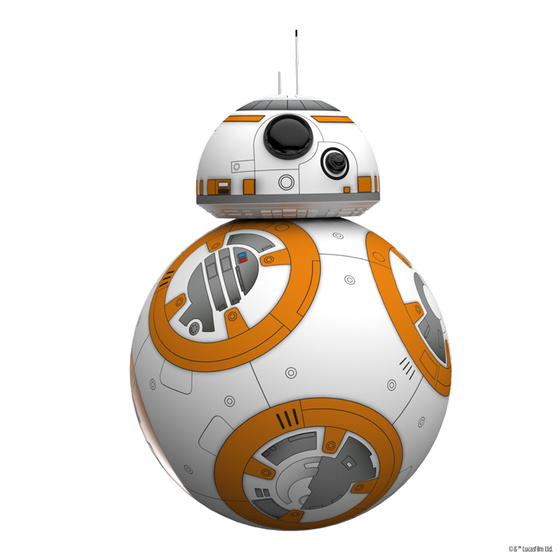
\includegraphics[scale=0.06]{robot}};
      \fill (1,-4)  rectangle (2,1);
      \fill (2,-3)  rectangle (3,0);%\atorig
	 \pgfmatrixnextcell
      \fill (-3,0)  rectangle (1,1);%\atorig2 
	 \pgfmatrixnextcell
      \fill (-1,-4) rectangle (0,-1);%\atorig3 
	 \pgfmatrixnextcell
      \fill (0,-1) rectangle (-1,-3);%\atorig4 
	 \pgfmatrixnextcell %ici pour un carré
      \fill (4,-3) rectangle (5,1);
      \fill (1,3.5) rectangle (6,2.5); 
      \fill (-1,0.5)  rectangle (4,1.5);%\atorig5
      \fill (3,-1) rectangle (4,-3);
	  \pgfmatrixnextcell 
	 \node[] at (-3,2) {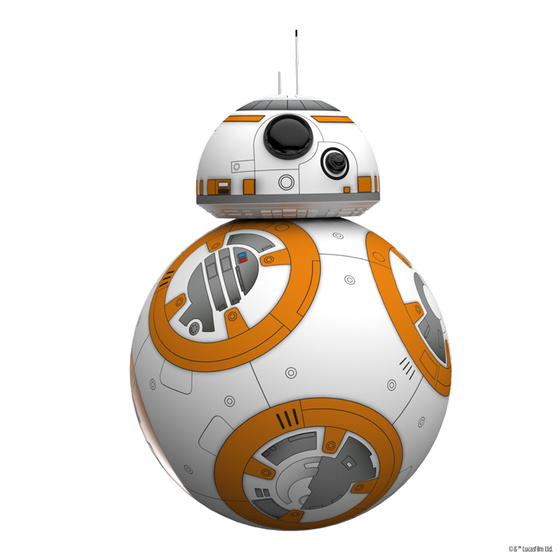
\includegraphics[scale=0.06]{robot}};
      \fill (0,-1)  rectangle (2,0);%\atorig6 
      \fill (-2,-2) rectangle (0,-1);
	  \pgfmatrixnextcell
      \fill (0,0)   rectangle (1,-4);%\atorig7 
	  \pgfmatrixnextcell
\node[] at (-2,-3) {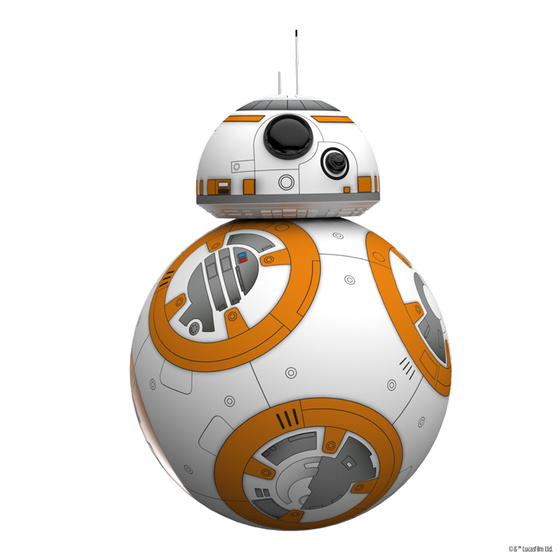
\includegraphics[scale=0.06]{robot}};
      \fill (1,-2) rectangle (2,2); \\
	   % \pgfmatrixnextcell
    }
\end{tikzpicture}
\caption{Robot example}
\label{fig:port}
\end{figure}
They must coordinate to keep away thieves from the cargo containers, by verifying regularly that no container has been opened. 
%Each robot must regularly ensure that each container is safe.
After chasing a thief outside the port, they have to drive back near containers that need the most to be checked.

Such a cooperating  team is called a distributed system \cite{Lynch96,Tel:2001:IDA:517021}. A system is distributed when it is composed of a set of autonomous computation entities endowed with communication abilities in order to solve a common task.
Traditionally, the entities have been assumed to be stationary and to communicate with each other thanks to message passing. 
The robot model we study in this thesis \cite{suzuki_distributed_1999,FPS12} differs from the classical one in two aspects: 
the entities are mobile and they do not communicate via message passing. Moreover, these mobile entities may be endowed with limited capabilities.
The concern in mobile robots research is to understand what kind of basic capabilities are needed for the robot team in order to accomplish a given task, in the absence of any central coordinating authority, and at what cost.
Several tasks have been investigated both in the plane or in a discrete environment.
Since these assigned tasks may be critical, it must be ensured that the robots accomplish them correctly, in spite of their limitations.

So far, robot networks have been either validated empirically or algorithm designers wrote handmade proofs. 
These proofs are hard to write and read, and reasoning on complex systems is both cumbersome and error-prone. 
Automated proofs on an abstract mathematical model of the system could remove the fastidious task of inspecting the system behavior to ensure its correctness with respect to a certain specification, \ie the definition of what  the system is expected to do, described by a set of properties.
Such techniques are called formal verification techniques.
Several approaches exist: 
\begin{description}
\item [Test\hfill] \index{Test} Test is probably the most frequently used method. In a first phase, execution scenarios whose results are known in advance have to be developed. The system is then executed in accordance with such a scenario and one can check if the output is as expected.
The presence of such tests does not guarantee the correctness of system behaviors outside the cases tested. Moreover, the design of adequate tests is more difficult for concurrent or distributed systems.
\item [Proofs\hfill] \index{Proof} In this approach, 
the semantics of a system (or a class of systems) is formalized in a mathematical language. Then the argument underlying a hand proof is formalized in the logic of a proof assistant and the proofs are checked mechanically.
Thus an expert user must interact to properly orient the proof construction. Besides, when a proof fails, the diagnostic is known to be difficult.
Various proof assistants have emerged since the 60’s: PVS\footnote{http://pvs.csl.sri.com}, Coq\footnote{https://coq.inria.fr/} and Isabelle/HOL\footnote{https://isabelle.in.tum.de} are among the most widely used.
\item [Model checking\hfill] \index{Model checking} The system and the properties to be verified must be first formalized, possibly abstracting away irrelevant details. An algorithm, which depends on the classes of models for the system and the properties, is then applied to check whether the properties are satisfied by the model. One advantage of this technique is its ability to extract behavior invalidating properties. Thus, it can be used at the design phase to validate prototypes. A drawback of this method is the so called combinatorial explosion: exploring all executions in a model of large size is time and memory consuming.
The model checkers \textsc{Uppaal}\footnote{http://www.uppaal.org} and \textsc{Spin}\footnote{http://spinroot.com/spin/whatispin.html} are amongst the most frequently used.
\end{description}
Each of these approaches has its strengths and drawbacks: While tests can be easy to implement, they cannot be applied in the design phase and the generation of exhaustive tests is a difficult problem; Proofs are difficult to implement since they require the presence of an expert, but they are exhaustive, applicable at the design phase, and
they can handle systems where some variables are not specified (like for instance the number of processes), called parameterized systems; 
Finally, the model checking approach is a comprehensive and automatic one but limited by the model size. 
Moreover, the problem is  undecidable in general for parameterized systems~\cite{apt.kozen.86}.


While the correctness of an algorithm can be verified at the design phase by model checking and assisted proof, 
another formal technique called synthesis aims at automatically generating a protocol from its specification. An advantage of this method is that the generated protocol is correct by design.
%The produced protocol is correct by designed.  
%Automatic synthesis is a more difficult problem since it produces a program that is . 
This question raised early interest~\cite{emersonclarke1981, MannaWolper84} and actually goes back to Church~\cite{Church62, BuchiLandweber69}. It is even more difficult when the program to generate is intended to work as an open system, maintaining an on-going interaction with a (partially) unknown environment. Given a specification, if there exists a program such that its behavior satisfies this specification, regardless of the environment behavior, then this program must be automatically built. Otherwise, it must be proved that the problem cannot be solved.

 It is known since \cite{BuchiLandweber69} that a successful approach consists in viewing the synthesis problem as a \emph{game} between the system and the environment. The system and its environment are considered as opposite players, the winning condition being the specification the system should fulfill. Then, the classical problem in game theory of determining winning strategies for the players is equivalent to finding how the system should act in any situation, in order to satisfy its specification, irrespective of how the environment behaves.
However, this problem is also undecidable in general for distributed systems~\cite{PnueliR90}. 
 \bigskip
 
 In this work, our aim is to investigate how formal methods can be applied in the context of mobile robot algorithms.
 We would like to bring out the benefits of these methods compared to traditional approaches.


\bigskip
%\todo{plan de l'intro}
In the next sections, we present the robot model considered in this manuscript, as well as existing work on the two main problems 
studied here: exploration and gathering by mobile robots. 
Then, we give a more detailed description of the formal methods devoted to the verification of mobile robots protocols. 



	\section{Mobile robots}
In this thesis, we consider a theoretic model \cite{suzuki_distributed_1999,FPS12}, where it is possible to express that robots with limited capabilities 
cooperate to achieve a common objective. 
In this model, each robot behavior is an infinite sequence of cycles where each cycle is divided into three phases: 
The Look phase, the Compute phase and the Move phase.  \index{Look-Compute-Move}
We first give a brief overview of these phases, restrictions are discussed in the next paragraph.
\begin{description}
\item [Look] The robot observes its environment ; the result of this operation is a snapshot of the positions of all robots within its radius of visibility with respect to its own coordinate system. 
\item [Compute] The robot executes the algorithm (the same for all robots), using the snapshot of the Look operation as input, the result is a  destination point given relatively to its coordinate system. 
 \item[Move] The robot moves toward the computed destination; if the destination is the current location, the robot stays still, performing a null movement. 
 \end{description}
 
This model called ATOM, also referred  in the literature as the SYm model, was proposed by Suzuki and Yamashita~\cite{suzuki_distributed_1999}.
 It was then refined by Prencipe~\cite{prencipe_new_2000} into a more realistic version called the CORDA model. 
 These models differ in their degrees of atomicity: 
\begin{itemize}%%%%%%%%%%%%%%%%%%%%%%%%%%%%%%%%%%%%%%%%%%here executes ? aver un subset ?
\item In the historical model, ATOM\index{ATOM}~\cite{suzuki_distributed_1999}, some non-empty subset of robots executes the three phases synchronously and atomically. This gives rise to two variants: Fsync, for the fully-synchronous model where all robots are scheduled at each cycle, and Ssync, for the semi-synchronous model, where a strict subset of robots can be scheduled. 

%Ssync
\index{Ssync}
In the semi-synchronous (Ssync) model, one or more robots are activated at each cycle, and obtain the snapshot corresponding to its observation, but all these snapshots are taken simultaneously and atomically. Based on that snapshot, they compute and perform their move. As a consequence, no robot will ever be observed while moving, and the understanding of the universe by the active robots is always consistent. In this case, the system behavior corresponds to executing all operations instantaneously (all Look/Compute operations immediately followed by all Move operations). 
%Note that such a system is equivalent to a synchronous system in which the chosen robots are activated simultaneously and all operations within a cycle are instantaneous. Indeed, the unpredictability is restricted to which robots are activated in each cycle (and the destination).
%Fsync
\index{Fsync}
The fully synchronous (Fsync) model is a particular case of Ssync, since in each cycle, all robots are activated. 
\item
The second model, CORDA~\cite{prencipe_new_2000}, \index{CORDA} also called Async\index{Async}, is a more realistic variant: In this less constrained model, each robot is activated asynchronously and independently from the other robots. Furthermore, the duration of each phase as well as the time between successive phases in the same cycle are finite but unknown. As a result, computations can be based on totally obsolete observations, taken arbitrarily far in the past. Another consequence is that robots can be seen while moving, creating further inconsistencies in robot views. 
\end{itemize}

A particular variant, between Async and Ssync, has been considered in~\cite{LinMA07a}. In this limited form of asynchrony, called partial Async, the time spent by a robot in the Look, and Compute phases is bounded by a globally predefined amount, while the time spent in the Move phase is bounded by a locally predefined quantity (not necessarily the same for each robot). 

Note that  in term of executions, Fsync is included in Ssync, and Ssync is included in Async.

\bigskip
The ability of a team to achieve an assigned task depends mainly on the capabilities of its robots:  the more powerful they are, 
the more easily the task is solved. %The concern in mobile robots research is to understand what kind of basic capabilities are needed for the robot team in order to accomplish a given task, in the absence of any central coordinating authority, and at what cost. 
 
%They are endowed with sensing, computing, and moving capabilities described below. 
\subsection{Robot weaknesses}
We now detail the minimal assumptions usually made on these robots.
%Anonymous and similar: 
\index{Anonymous}
The robots are identical and anonymous, they execute the same algorithm and they cannot be distinguished using their appearances, but they can have different computing speeds and different moving speeds (in the Async case). Robots may have identities but neither they nor the other robots have knowledge or access to these identities. 
%know or can have access to these, only an omniscient observer has this knowledge.

%oblivious
\index{Oblivious}
The robots are oblivious \ie they have no memory of their past actions. 
%their actions do not depend on previous actions. 
This capability implies that any state can be considered as initial. Hence, robot algorithms will have self-stabilization\index{self-stabilization} properties: 
A self-stabilizing distributed protocol ensures that a correct behavior can be recovered in a finite time without any external or manual help.
%In~\cite{DieudonneP12}, Dieudonne et Petit discuss on the link between the mobile robot model and self-stabilization.

%no common handiness: 
\index{handedness}
\index{chirality}
Robots  have neither a common sense of direction, nor a common handedness (chirality).
Each robot has its own unit of length and a local compass defining his own local Cartesian coordinate system. This local coordinate system is self-centric, \ie the origin is the robot's position. Moreover, the local coordinate system of oblivious robots may completely change during their life. However, it remains invariable during a cycle.

%no communication; other works communication: via msg, pebbles, ...
\index{Communication}
The robots are silent: there is no communication via message passing.
They communicate by observing other robots positions, and taking a decision accordingly. In other words, the only mean for a robot to send information to some other robot is to move and let the others observe.


\subsection{Robot capabilities}
To execute their Look-Compute-Move cycles, the robots are endowed with sensing, computing and moving capabilities. These capabilities 
depend on the environment that can be continuous or discrete.
%anissa
Two cases have been studied in the literature: 
\begin{itemize}
\item The continuous euclidean space \cite{suzuki_distributed_1999,FPS12}, in which the robots entities move on a plane, \index{Continuous space}
\item The discrete universe~\cite{KlasingMP06,flocchini_computing_2007}, in which space is represented by a graph, where nodes correspond to the possible locations and edges to the routes for a robot from one location to another.\index{Discrete space}
\end{itemize}
The discrete representation is motivated by practical aspects with respect to the unreliability of sensing devices used by the robots as well as inaccuracy of their motorization~\cite{CDDMJ08j}.  A discrete setting permits to approximate these features and simplify the design of robot models by reasoning on finite structures. However, it is more sensitive to the size of constants, which may significantly increase the number of symmetric configurations 
when the underlying graph is also symmetric (\emph{e.g.} a ring) and thus the size of correctness proofs~\cite{ASN11c, KLOT11, KLOT12}.


\subsubsection{The sensing capability}
\index{Visibility}
 Robots are endowed with visibility sensors providing the locations of other robots. The obtained location is either fine grained (which means that it has been obtained with some degree of accuracy) or coarse grained (robots can only be observed at some specific discrete locations, each location being adjacent to one another). In the first case, the literature mostly refers to the continuous space model, while in the latter case, it is the discrete one.
 
Robots are dimensionless and thus their visibility cannot be obstructed:  if three robots $r_1$, $r_2$, and $r_3$ are aligned, with $r_2$ in the middle, $r_1$ can see $r_3$. Moreover, robots may share the same position: this is called a \emph{multiplicity point} or a \emph{tower} \cite{FPS12}. The ability for a robot to detect multiplicity is crucial to achieve some particular tasks. We distinguish weak and strong multiplicity detection. 
\begin{itemize}
\item The weak multiplicity detector detects whether there is zero, one or more than one robot at a particular location. 
\item The strong multiplicity detector senses the exact number of robots at a particular location. 
\end{itemize}
This sensor may be local or global: in the local setting a robot only detects multiplicity at its current position, while in the  global setting the multiplicities of all positions are known by all robots.

A third characteristic of robot sensing capability is their visibility radius. It can be infinite \ie a robot is able to sense the position of all other robots, or finite \ie there exists a bound (expressed as a distance) beyond which a robot cannot sense anything.
Note that the sensing is defined in the robot’s own coordinate system.

\subsubsection{The computing capability}
As in classical distributed systems, robots are assumed to be able to perform any finite sequence of computing steps in negligible time. 
Since robots are oblivious, volatile memory is used to perform computing tasks in a single Look-Compute-Move cycle, but the memory content is erased at the end of each cycle.
The computation takes as input the observation made in the Look phase and gives the robot a move.
When two robots are on the same location or are symmetric, they should be given the same move.
In some instances, when the robot observation does not permit to distinguish directions, the computed location may be ambiguous: it then corresponds to a non deterministic move, which can be resolved by a scheduler.

\subsubsection{The moving capability}
Robots may move only to the location provided by the computing phase of the current cycle.  
% and is thus decided by an adversary. 
In the discrete space model, a robot may move only to a location that is adjacent to its current location. In the continuous space model, a robot moves toward its computed destination. %Such a robot may be interrupted by an adversary before it finishes its move.



%schedulers %%%%%%%%%%%%%%fairness%%%%%%%%%%%%
\subsubsection{Scheduling}
\index{Fairness}
When several processes execute concurrently, scheduling plays an important role: Schedulers are abstractions used to characterize the degree of asynchrony in the robot network \cite{DefagoGMP06,FPS12}. Various notions of fairness with various names are used in the areas of distributed algorithms and verification. We define several of them below.
We call "unconditionally fair" the most general scheduler that activates every robot infinitely often, in order to avoid starvation. In this case, some robots may be activated arbitrarily more than other. The $t$-bounded scheduler ensures that, between any two activations of a given robot, every other robot is activated at most $t$ times. So the ratio between the fastest and the slowest robot is at most $t$. 

There are  other types of fairness which depend on the scheduling of actions. 
An action that can be performed in the current  state of a robot is called \emph{enabled}. The \emph{Strongly Fair} scheduler ensures that every action that is infinitely often enabled should be executed infinitely often, the \emph{Weakly fair} scheduler ensures that every action that is continuously enabled  from some point on should be executed infinitely often.
 

		\subsection{Other variants of robots}
In the literature, weaker robots than those described above have been studied.
\subsubsection{Limited visibility}
%avec obstruction

Limited visibility has been studied when robots are myopic~\cite{AndoOSY99,FPSW05j, GuilbaultP11,DattaLLP13}.\index{Myopic robots} A myopic robot cannot see the nodes located beyond a certain fixed distance. The strongest myopia corresponds to when a robot can only see robots located at its own and at neighboring locations. Note that the weakest myopia is when the myopia distance is the diameter of the graph, this corresponds to an infinite visibility.	

An other way to describe limited visibility is by considering an environment where the line of sight of a robot is obstructed by the closest robot on that line. This is typically assumed in (and is the main motivation for) the study of robots that are solid (i.e., with a physical dimension)~\cite{ChaudhuriM15,CzyzowiczGP09,HPT14}. 
%Solidity does not always imply obstructed visibility; it is conceivably possible that the snapshot contains the positions of all the robots even if they are solid %(e.g., in case the snapshot is provided by a satellite); the case of solid but transparent robots has been examined in~\cite{DattaDCM13}.


%a robot might not even know the total number of robots nor where they are located if outside its radius of visibility




	
\subsubsection{Faulty robots}\index{Byzantine robots}
Usually robots are assumed to operate without failures (those robots are called correct). Yet, some unexpected behaviors may occur. In the worst case, robots are Byzantine, meaning that they can behave arbitrarily. 
A less serious fault is the crash fault, where a robot unexpectedly stops moving forever.
Fault-tolerant algorithms for gathering were studied in~\cite{AgmonP06,DefagoGMP06,CourtieuRTU15}.	
		%voir papier Xavier urbain
		%Cédric Auger, Zohir Bouzid, Pierre Courtieu, Sébastien Tixeuil, and Xavier Urbain. Brief announcement: Certified impossibility results for byzantine-tolerant mobile robots. In Yehuda Afek, editor, International Sympo- sium on Distributed Computing (DISC), volume 8205 of Lecture Notes in Computer Science, pages 577–578, Jerusalem, Israel, October 2013. Springer.	
%voir le rapport technique de Maria

\bigskip 
In this thesis, we focus on the discrete universe and study two main problems for asynchronous, identical, and oblivious robots: The gathering problem~\cite{KlasingMP06,klasing_taking_2008}, where robots must all reach a common given location, and the exploration problem~\cite{flocchini_computing_2007,devismes_optimal_2010-1}, where the robots must visit all locations. In the next section, we informally describe existing algorithms for these two problems. 

\section{Gathering and exploration}
One of the benchmarking problems for mobile robots is \emph{gathering}~\cite{markoubook} (also known as the \emph{Rendez-Vous} problem). This problem was the first studied in the literature: robots have to move in such a way that they eventually reach the same position, not known beforehand, and remain there thereafter. 
Similarly to the Consensus problem in conventional distributed systems, where all entities must agree on a same value, gathering has a simple definition but the existence of a solution greatly depends on the synchrony of the system and on the initial configuration. 


The gathering problem draws its significance from the fact that it permits to obtain a common coordinate system.
 If  the robots can gather at a single point, then they can subsequently agree to use that point as the origin of the common coordinate system. %Formation of a circle implies agreement on both the origin and the unit distance (i.e., the center and the radius of the circle). %Formation of a symbol $T$ implies agreement on the origin, the unit distance, and a direction.
 In the sequel we discuss the results obtained in the plane and in the discrete environment.
A survey discussing how varying assumptions influence feasibility and complexity of gathering under different environments is presented in~\cite{Pelc11}.


%plane
\subsection{Gathering in the plane}
The gathering study begins with Suzuki and Yamashita~\cite{suzuki_distributed_1999} who propose a gathering algorithm for 
non-oblivious robots in a continuous Euclidean space, with a synchronous model. They proved that gathering cannot be solved with two oblivious robots: All configurations are symmetric and may lead to robots endlessly swapping their positions. 
However, Défago \textit{et al.}~\cite{DefagoGMP06} propose probabilistic algorithms in the ATOM model without any additional assumption.
These algorithms permit to gather two robots with a fair scheduler, and any number of robots with a $t$-bounded scheduler.

Even if there is no deterministic algorithm for the gathering of two robots,  the problem can be solved for three or more robots if there are no towers in the initial configuration: at each step, either the robots remain symmetric and they eventually reach the same location, or the symmetry is broken and this is used to move one robot at a time. Suzuki and Yamashita~\cite{suzuki_distributed_1999} propose an algorithm that exploits the properties of the center of gravity (sometimes called the center of mass, the barycenter, or the average) of the team.
%They conjecture that for any number of robots an easy solution would be to gather the robots at the Weber point: The unique point in the plane that minimizes the sum of the distances between itself and all the points in a given set of points.  An interesting property of the Weber point is that it does not change when moving any robot towards it. Unfortunately, the Weber point is not computable~\cite{WB1969}.

When robots are asynchronous there might be various oscillatory effects on the computing of the center of gravity, preventing robots from moving towards each other and possibly even causing them to diverge and stay away from each other in certain scenarios.

Prencipe~\cite{Prencipe05} studied the problem of gathering in both synchronous and asynchronous models. He proved that the problem cannot be solved in Async without additional assumptions. The idea of this impossibility result is that from any initial configuration and for any algorithm with $k\geq3$ robots, there exists an asynchronous scheduling producing a configuration where the set of robots are gathered into two different locations, reducing the problem to gathering with two robots. 
Moreover, Défago \textit{et al.}~\cite{DefagoGMP06} prove that, without additional assumption, there is no deterministic algorithm for the Async gathering even under a $t$-bounded scheduler. They propose a probabilistic algorithm to gather $k\geq2$ robots under a $t$-bounded scheduler.

Therefore, to solve the gathering problem in Async, some additional assumptions must be made.
Cieliebak~\cite{CieliebakP02,cieliebak_solving_2003} proposes to add weak global multiplicity detectors to the robots, or to use 
non-oblivious robots~\cite{Cieliebak04}.
In~\cite{CieliebakP02},  some algorithms are presented for 3 or 4 robots, that % and more
handle all initial configurations without tower. 
%%3
%The algorithm for 3 robot $r_1$, $r_2$, $r_3$ is the following: 
%If the robots are on a line, the two outer robots move towards the median robot. 
%If the triangle formed of $r_1$, $r_2$, and $r_3$ contains an angle of at least $120\degree$ in vertex $r_i$, then the other two robots move  towards $ri$. Otherwise, the triangle contains no angle greater than or equal to $120\degree$, and all robots  move towards the center of equiangularity of $r_1$, $r_2$ and $r_3$ .(The center of equiangularity $c_e$ is the unique point such that moving toward this point does not change the center of equiangularity, and the angles: $r_1,c_e, r_2$, $r_1,c_e, r_3$ and $r_2,c_e,r_3$ are equal to $120\degree$.)
%%4 %pareil 
%%5++
%pour 5 plusieurs algo mais qui ne marche pas car ils ne savent pas comment éviter conf periodic.... donc ok en sync mais pas Async
The algorithm in~\cite{cieliebak_solving_2003} permits to gather 5 or more robots.
The general idea on which these algorithms are based is to let the robots reach a configuration where there is exactly one location $\ell$ in the plane with multiplicity greater than $1$. When such a configuration is reached, all the robots move towards $\ell$ avoiding collisions (i.e., $\ell$ remains the only point with a tower).
%In~\cite{Cieliebak04} the author proposes a gathering algorithm for two or more non-oblivious robots.
%ils précalculent un point de rdv...


	%%limited visibility
The gathering problem was also studied in a system where the robots have limited visibility~\cite{FPS12}.
Ando \textit{et al.}~\cite{AndoOSY99} present an algorithm allowing the convergence (towards a common point, without ever reaching it) in the Ssync model. Other gathering algorithms are proposed in Ssync, for more powerful robots~\cite{SouissiDY09}.\\
In the asynchronous model, the problem becomes solvable if the robots have a common coordinate system (agreement on axes and directions of a common coordinate system, but not necessarily on the origin nor on the unit distance)~\cite{FPSW05j}, then they can gather without multiplicity detectors even when the visibility is limited. %The propose algorithm does not  take into account configurations where a robot has no other robots in its circle of visibility.%
%In partial Async convergence in possible even with limited visibility~\cite{LinMA07a}.

	%%fault tolerance
Fault-tolerant algorithms for gathering were studied in~\cite{AgmonP06,DefagoGMP06}.
For the gathering problem, in a crash-prone system, there is no deterministic algorithm under a fair $t$-bounded scheduler, and there is no probabilistic algorithm under a fair scheduler.
However, in~\cite{DefagoGMP06} a probabilistic algorithm that solves the gathering under a $t$-bounded scheduler has been proposed. 
When only non-faulty robots must gather, there is neither a probabilistic nor a deterministic algorithm that solves the gathering problem, for $k\geq3$ robots when more than 2 crash faults happened, under a fair scheduler. But with only one crash Agmong \textit{et al.}~\cite{AgmonP06} present an algorithm in the asynchronous model under a fair scheduler. %In a crash-prone system, there is an algorithm that probabilistically solves the weak gathering problem, when there is more that 2 faults, under an unfair scheduler if robots are aware of the system multiplicity~\cite{DefagoGMP06}..

 For Byzantine faults, in Ssync it is impossible to gather all non-Byzantine robots, even in the presence of a single Byzantine fault. In Fsync an algorithm is provided for gathering all non-Byzantine robots with up to $f$ faults, when the number of robots $k$ is at least $3$ and when $k \geq 3f + 1$.
 In~\cite{DefagoGMP06}  a probabilistic algorithm that solves the gathering of all non-Byzantine robots is proposed. This algorithm requires a $t$-bounded scheduler and robots endowed with strong global multiplicity detectors.
%%voir aussi
%Gathering Despite Mischief (	Yoann Dieudonné,Andrzej Pelc	,David Peleg)



\subsection{Gathering in the discrete environment}
%Discrete
In the discrete environment, gathering  has been studied in various environments: trees \cite{FraigniaudP08}, grids~\cite{DAngeloSKN12}, rings~\cite{KlasingMP06,klasing_taking_2008}, and general graphs~\cite{DessmarkFKP06}. 
In the sequel we are only interested in the ring topology: The ring network is particularly intricate since its regular structure induces a number of possible symmetric situations, from which the limited abilities of robots make it difficult to escape. 
In order to work in the most challenging context, the ring is non oriented and anonymous (neither nodes nor links of the ring have any labels). In the initial configuration, however, there is no tower.
%Without any multiplicity detection, in~\cite{DAngeloSKN12,DAngeloDSN12} the grid and the tree topologies have been fully characterized.

In the discrete setting and more particularly in the ring, we use informal notions 
of symmetric and periodic organizations of robots, precise definitions are given in the next chapter. 
\begin{example}
In the ring configuration depicted in Figure~\ref{fig:introEx}, a white node represents a free location, and a grey node a location occupied by a robot.
The first ring configuration is symmetric and the rightmost one is periodic \ie invariant by non-trivial rotation.
\begin{figure}[h] % robot tous du même gris
\centering
	\subfloat[][symmetric
	]{
			\centering 
			\begin{tikzpicture}[node distance =15em,>=stealth, thick] 
			\node[circle,minimum size =8em, draw, thick] (C){};
			\foreach \i in {0,...,10}\node[circle,minimum size
			=1em,draw,fill=white,thick]at(\i*32.5: 1.6) (\i){};
			\node[circle,minimum size =1em,fill=gray!60]at(4*32.5: 1.6) (17){};
			%\node[]at(7*36: 1.65) (1721){{$r_1$}};
			\node[circle,minimum size =1em,fill=gray!60]at(5*32.5: 1.6) (17){};
			%\node[]at(9*36: 1.65) (1721){{$r_2$}};
			\node[circle,minimum size =1em,fill=gray!60]at(1*32.5: 1.6) (18){}; 
			%\node[]at(2*36: 1.6) (181){{$r_3$}}; 
			\node[circle,minimum size =1em,fill=gray!60]at(8*32.5: 1.6) (29){};
			%\node[]at(4*36: 1.65) (191){{$r_4$}}; 
			
			\node[]at(4.5*32.5: 1.4) (i){};
			\node[]at(10*32.5: 1.45) (ii){};
			\draw (i) -- (ii);

			

			\end{tikzpicture}
	}\hspace{0.5em}
\subfloat[][periodic
	]{
			\centering 
			\begin{tikzpicture}[node distance =15em,>=stealth, thick] 
			\node[circle,minimum size =8em, draw, thick] (C){};
			\foreach \i in {0,...,14}\node[circle,minimum size
			=1em,draw,fill=white,thick]at(\i*24: 1.6) (\i){};
					
			\node[circle,minimum size =1em,fill=gray!60]at(3*24: 1.6) (1){};
			\node[circle,minimum size =1em,fill=gray!60]at(4*24: 1.6) (1){};
			\node[circle,minimum size =1em,fill=gray!60]at(6*24: 1.6) (2){};
			\node[circle,minimum size =1em,fill=gray!60]at(8*24: 1.6) (3){};
			\node[circle,minimum size =1em,fill=gray!60]at(9*24: 1.6) (3){};
			\node[circle,minimum size =1em,fill=gray!60]at(11*24: 1.6) (4){};
			\node[circle,minimum size =1em,fill=gray!60]at(13*24: 1.6) (5){};
			\node[circle,minimum size =1em,fill=gray!60]at(14*24: 1.6) (5){};
			\node[circle,minimum size =1em,fill=gray!60]at(1*24: 1.6) (6){};

					

			\end{tikzpicture}
	}
	\caption{Particular configurations}
	\label{fig:introEx}
\end{figure}

\end{example}


The gathering problem on a ring was first investigated by Klasing \textit{et al.}~\cite{KlasingMP06}.
%impossibility results in Fsync
They prove that gathering 2 robots is impossible on any ring, and gathering any number $k > 2 $ robots is impossible without additional assumptions. Proofs of these impossibility results are similar to those in the plane.
A more specific impossibility result is that even if robots are endowed with multiplicity detectors, gathering is impossible for a particular 
class of symmetric configurations. In the sequel we only discuss results given in the Async model.
%explication periodic
%explication edge-edge

In Async, when robots are endowed with weak global multiplicity detectors, %if initial configurations does not contain any multiplicity, the gathering problem is simpler because it is sufficient for a protocol to ensure that a single multiplicity point exists to have all robots gather in this point, so it reduces the gathering problem to the creation of a single multiplicity point. 
the proposed protocols either exploit the symmetries~\cite{klasing_taking_2008} or try to avoid them, and break them when encountered~\cite{KlasingMP06}.
In~\cite{KlasingMP06} the protocol handles only an odd number of robots and starts from any tower-free configuration that is not periodic. 
 %The idea of the proposed solution was to create a single multiplicity which will be the gathering node.
In~\cite{klasing_taking_2008}, the authors provide an algorithm for gathering 18 or more robots on the ring, from any initial configuration not concerned by the impossibility results.
For these initial configurations and less than 18 robots, a number of ring gathering algorithms have been proposed in the literature~\cite{navarrasirocco2011,navarradisc2012,navarraipdps2013,navarrasirocco2013}. They apply to various cases according to 
the size of the ring, the number of robots and the subclass of initial configurations. When multiplicity detection is available a unified 
strategy was proposed in~\cite{navarradisc2012}. 
%In~\cite{ASN11c} the authors address the problem of 6 robots and provide a distributed algorithm that gathers the robots when starting from any symmetric configuration of type node-edge, or node-node.

%%25=
%%23=
%Most of the cases with 4 robots have been solved in [25]. The cases left open in [25], referred to as the set SP4, are symmetric configura- tions of type node–edge with 4 robots and the odd interval cut by the axis bigger than the even one, with an interval being a maximal set of empty consecutive nodes. In general, configurations in SP4 are ungatherable as outlined in [23] for configurations of 4 robots on a five nodes ring. Actually, spe- cific configurations in SP4 could be gatherable but requiring suitable strategies difficult to be generalized. The main diffi- culty faced when dealing with configurations in SP4 comes from the fact that among the two intervals cut by the axis, the odd one is bigger than the even one.

%robots avec local multiplicity detectors
In~\cite{IIKO10c, KLOT11, KLOT12} the authors achieve similar results with weak local multiplicity (robots are not able to see nodes that contain multiple robots unless it is their current node). 
The algorithm by Izumi \textit{et al.}~\cite{IIKO10c} assumes that initial configurations are neither symmetric nor periodic, and the number of robots is less than half the number of nodes. 
For an odd number of robots, %or odd number of nodes in the same model, 
Kamei \textit{et al.}~\cite{KLOT11} propose an algorithm that also works from initial symmetric configurations. 
For an even number of robots on an odd-sized ring, Kamei \textit{et al.}~\cite{KLOT12} propose an algorithm for non periodic initial configurations. %are not periodic. % il y a encore le papier~\cite{navarra2014} des algo pour des conf init particuliéres maid rien d'unifié
An algorithm that achieves the gathering for any initial configuration (when it is possible) is presented in~\cite{DAngeloSN14}: 
it uses existing algorithms as subroutines for the basic solvable cases with 4 or 6 robots from~\cite{4Rob} and~\cite{ASN11c} respectively.

%robots with labels or tokens
%-> similaire à de la communication ou de la mémoire on ne s'en occupe pas

%%limited visibility
%Gathering Asynchronous Oblivious Agents with Local Vision in Regular Bipartite Graphs: In [GP11], the authors studied the gathering problem considering robots having only a local visibility i.e., they can only see robots located at its own and at adjacent nodes. Under this assumption, the authors provide a complete solution of the gathering problem for regular bipartite graphs. They first characterize the class of initial configurations allowing to solve the gathering problem on such graphs, and they propose a gathering algorithm assuming that the system starts from a configuration in this class.
%B. Degener, B. Kempkes, T. Langner, F. Meyer auf der Heide, P. Pietrzyk, and R. Wattenhofer. A tight runtime bound for synchronous gathering of autonomous robots with limited visibility. In Proc. of the 23rd ACM Symp. on Parallelism in algorithms and architectures (SPAA), pages 139–148, 2011.

%%other
%Multiple Agents RendezVous in a Ring in Spite of a Black Hole
%Stefan Dobrev,(black holes) Paola Flocchini, Giuseppe Prencipe, Nicola Santoro
 

\subsection{Exploration}
Exploration is the process by which every location of a \emph{discrete} environment is visited by at least one robot. 
%Due to its definition it must take place in the discrete environment. 
The proposed algorithms mostly try to obtain a common sense of orientation:  the intuition is to arrange the robots in a particular shape, which will allow them to have a common sense of direction, and then to define a direction to explore successfully their environment.
%Like the gathering, the exploration is impossible if the initial configuration is periodic~\cite{flocchini_computing_2007}.
The problem of exploration has several variants, among them the exploration with stop and the perpetual exploration problem.
Both problems are unsolvable if the initial configuration is periodic~\cite{flocchini_computing_2007}.

The study of the exploration begins with the exploration with stop~\cite{flocchini_computing_2007}: 
Robots achieve an exploration with stop if regardless of their initial location, the robots reach a configuration in which they all remain idle and 
each node has been visited by a robot. The difficulty of this task arises from the fact that robots need to stop after all locations have been explored. It requires robots to “remember” how much of the graph was explored: Since they have no persistent memory, this means that they must be able to distinguish between various stages of the exploration process. 
 
Exploration with stop has been studied for paths~\cite{FlocchiniIPS11}, trees~\cite{FlocchiniIPS10}, grids~\cite{devismes_optimal_2011}, rings~\cite{flocchini_computing_2007} and general graphs~\cite{ChalopinFMS10}.
We focus again here on ring topologies, where the problem was studied only for robots endowed with strong global multiplicity sensors.
Flocchini is the first to study this problem in a ring~\cite{flocchini_computing_2007}, she presents an algorithm that permits the exploration with stop for any $k \geq 17$ robots starting from any configuration without multiplicity and where the size of the ring and the number of robots are coprime. The idea is that if $n$ and $k$ are coprime then no periodic configuration can happen.
 Devisme \textit{et al.}~\cite{devismes_optimal_2010-1} prove that there is no exploration protocol (even probabilistic) of an $n$-node ring with three robots for every $n > 3$. 
 Moreover, there exists no deterministic protocol that can explore an even sized ring with $k \leq 4$ robots~\cite{lamani_optimal_2010}: 5 robots are necessary and sufficient when the ring size is even, and 5 robots are sufficient when the size of the ring is odd.
 In~\cite{lamani_optimal_2010} the authors also propose an Async algorithm for 5 robots in an $n$-node ring where $n$ is coprime with five. The proposed algorithm is optimal in the number of robot moves.  
 
 Probabilistic algorithms for the exploration with stop have been studied by Devismes \textit{et al.}~\cite{devismes_optimal_2010-1}.
 This work shows that four identical probabilistic robots are necessary and sufficient in the Ssync model, also removing the coprime constraint between the number of robots and the size of the ring.  A probabilistic protocol is given for $4$ robots to explore any ring of size at least $4$, and a proof that no protocol exists with three robots is given.
 
 %limited visibility
 The case where robots with limited visibility explore an $n$-size ring has been studied by Datta \textit{et al.}~\cite{DattaLLP13}.
When robots have a visibility of 1, the exploration problem is not solvable with deterministic algorithms in Ssync (hence in Async). Even in Fsync, the exploration problem cannot be solved with less than 5 robots when the ring size is more than 6. 
 When they have a visibility of 3, no exploration is possible with less than 5 robots and a ring of size at least 13 in Ssync (and Async).
 In these conditions where the visibility is limited, several algorithms are proposed: 
 \begin{itemize}
 \item Two solutions in the Fsync model, when the visibility is 1: with a minimal number of robots for $3 \leq n \leq 6$ and for $n > 6$.
 \item Two solutions in the Async model, when the visibility is 2: with $7$ robots (for $n > 7$) and $9$ robots (for $n >19$).
 \item  Two solutions in the Async model, when the visibility is 3, with $5$ and $7$ robots.
 \end{itemize}
 %All algorithms work assuming that each robot is at distance at most φ of another one. Both solutions for 7 robots with φ = 2 and 5 robots with φ = 3 work starting from specific configurations.~\cite{exploration with oblivious myopic robots}


%\subsubsection{Exclusive perpetual exploration}
%Perpetual exclusive graph searching: Given a n-node graph G where all edges are contaminated, the graph searching problem consists in coordinating a team of robots to eventually clear all edges. The robots occupy the nodes of G and a robot can move along an edge from its current position to a neighboring node. An edge is cleared by a robot when it traverses it or if both its ends are simultaneously occupied by some robots.
The more difficult problem of exclusive perpetual exploration has been studied recently: 
Robots achieve an exclusive perpetual exploration if regardless of their initial (tower-free) location, each node has been visited by a robot infinitely often and no multiplicity point appears. The latter happens as soon as a moving robot collides with another robot, moving or stationary.
%: this happens when, while moving, it occupies the same location at the same time as another robot. 
 In this context, collisions are considered as undesirable events (with possibly negative consequences), and thus to be avoided. This is expressed by the \emph{exclusivity property}, which states that any node must be occupied by at most one robot.
%Recall that the only time robots are aware of other robots is during the Look phase. In particular, the robots have no way to detect the 
%position of other robots while moving.This means that collision avoidance must be done algorithmically.

Exclusive perpetual exploration has been studied in rings~\cite{blin_exclusive_2010,navarraipdps2013}, grids~\cite{bonnet_asynchronous_2011,baldoni_solvability_2008}, toruses~\cite{devismeshal}, trees~\cite{BlinBN12} and general graphs \cite{baldoni_anonymous_2008,BlinBN13}. 
Blin \textit{et al.}~\cite{blin_exclusive_2010} investigate both the minimal and the maximal number of robots that are necessary and sufficient to solve the exclusive perpetual exploration problem. They also propose algorithms for these two cases:
\begin{itemize}
\item For the lower bound, they prove that 3 robots are necessary and sufficient, provided that the size of the ring is at least 10, and show that no protocol with 3 robots can exclusively perpetually explore a ring of size less than 10. 
\item For the upper bound, they prove that $k = n - 5$ robots are necessary and sufficient to exclusively perpetually explore a ring of size $n$ when $n$ is co-prime with $k$.
\end{itemize}


A more generic algorithm has been proposed in~\cite{navarraipdps2013}: 
starting from any  tower-free configuration that is neither periodic nor symmetric, a ring of size at least $10$ can be perpetually explored by at least $5$ robots. The algorithm does not cover the case of $5$ robots exploring a ring of size $10$. 
% The case where 5 robots want to explore a ring of size 10 is not handled.
Combination of the results in~\cite{blin_exclusive_2010,navarraipdps2013}, leaves open the exclusive perpetual exploration of a ring of general size $n$ by 4 robots.

%Bonnet \textit{et al.} \cite{francois_bonnet_ideal_2012} studied a more difficult version of the exclusive perpetual exploration, 
%where each robot must visit infinitely often all nodes.  
%They prove that sometimes it is impossible even if as a team the robots achieve the perpetual exploration each node is infinitely often visited, 

\bigskip

All the algorithms described above have only been given handmade proofs, some of them rather sketchy. 
In the next section, we present cases where automated proofs were provided.
%Moreover, most of the time only sketches of these proofs have been given. 
%For such critical system the need of for formal verification is well established.

	
%%%%%%%%%%%%%%%%%%%%%%%%%VERIFICATION%%%%%%%%%%%%%%%%%%%%%%%%%%%%%
	\section{Formal Methods for robot algorithms}
Formal methods require mathematical representations of the system and its specification, given as a set of properties.
A distributed system is often described as a global transition system~\cite{Tel:2001:IDA:517021, DBLP:books/mk/Lynch96},
obtained by a composition of models of its sub-systems. 
%The specification can also be expressed by 
 %The set of properties given as its specification. 
 Properties can be classified into various types, among them 
 the well known safety and liveness properties. Safety properties informally require that ``something bad will never happen'', 
 like absence of deadlock. Invariants form an important subclass of safety properties, expressing that ``something is true at every step in every execution''.
 Liveness properties require that ``something good eventually happens'', for example there will be no starvation.
%
%We consider here transition systems for Sub-entities and we use them 
%in this work to represent sub-entities of the system. 
%The complete system is then obtained by a synchronized product of these transition systems. 
%
%Specification of the problem gives the algorithm required properties. for linear-time properties
In the context of linear-time properties, considered in this work, every possible specification can be written as the conjunction of safety and liveness properties~\cite{AlpernS85}.%%%%%%%%%%%%%%%%%%%%%%%%%%%%here%%%%%%%%%%%%%%%%%%%%%%%%%%%%%%%%%%%%%

In this section we present model checking, proof and synthesis, as well as related work for the use of these approaches in the context of 
mobile robot protocols.
		

\subsection{Model checking} \index{Model checking}
A model checker takes as input a model $M$, often in the form of a transition system, describing all possible executions of the system, and the property to be checked, expressed as a logic formula $\varphi$. It answers whether the model satisfies or not the formula. When the property is not satisfied, the model checker returns a counterexample, \textit{i.e.}, an execution of the model invalidating the property. This counterexample is useful to find errors in complex systems. This is an advantage of model checking compared to the other formal methods, such as theorem proving: 
In interactive proofs, one may fail to prove a property without finding out if the property is false or if one just didn't find the proof. 
%Still, some automatic techniques (including satisfiability solving) may be able to disprove a property by constructing a (counter-)model, which %corresponds to a counter-example.%which can disprove a property but without systematically providing such a counterexample. 

%\todo{The automata approach}
The automata approach for model checking was introduced by Vardi \textit{et al.} \cite{vardi_automata-theoretic_1986} to provide a unified and extensible framework, initially applied  to a class of logic formulas called \textsf{LTL} (described later in more details).
This approach splits the verification process of an \textsf{LTL}  formula into three operations: 
\begin{itemize}
\item The language $\mathcal{L} (M)$ associated with $M$ represents all possible executions of $M$. The formula $\varphi$ is translated into an automaton $\mathcal{A}_{\neg \varphi}$ whose language, $\mathcal{L}(A_{\neg \varphi})$, is the set of all executions invalidating $\varphi$.
\item Automata $M$ and $\mathcal{A}_{\neg \varphi}$ are synchronized to obtain an automaton $M \times \mathcal{A}_{\neg \varphi}$ whose language $\mathcal{L}(M \times \mathcal{A}_{\neg \varphi}) = \mathcal{L} (M) \cap  \mathcal{L} (\mathcal{A}_{\neg \varphi})$, is the set of executions of $M$ invalidating $\varphi$.
\item Finally the model checker performs an emptiness check on this product. The model $M$ satisfies $\varphi$ if and only if $\mathcal{L} ( M \times \mathcal{A}_{\neg \varphi}) = \emptyset$. If the emptiness check succeeds, it means that no execution invalidates $\varphi$, hence the property corresponding to $\varphi$ is satisfied by $M$. Otherwise, an execution of $M$ invalidating $\varphi$ is produced as a counterexample.
\end{itemize}		

The drawback of this method is the so-called combinatorial explosion problem~\cite{Valmari96} 
caused by the large size of the product $M \times \mathcal{A}_{\neg \varphi}$. 
The construction of $A_{\neg \varphi}$ is exponential in the size of $\varphi$. Moreover, 
starting from a system of concurrent processes, the automaton $M$ of the system has a size exponential in the number of processes. Consequently, in the automata-theoretic approach the synchronous product is often too large for the emptiness check to be performed in a reasonable execution time and memory.	

Distributed systems are naturally structured as a combination of components, among which several exhibit similar behaviors. Such components are said to be symmetric, and knowing the behavior of one such component is often sufficient to know the behavior of the combination. More formally, the symmetries of the system define an equivalence relation over its states. This relation can be used to produce a reduced state space, where at least one state per equivalence class is kept.
If exactly one representative state per class is kept, then maximal reduction is achieved. The definition of symmetries guarantees that the reduced state space preserves properties, if these properties also cannot distinguish between symmetric executions~\cite{ClarkeJEF96, EmersonS96}. This reduction is usually exponentially smaller than the original state space, thus reducing the execution time and memory of the verification process.

%%%utilisation de its
% Such methods aim to minimize the impact of the graph's size on the performance of model checking algorithms, especially by using concise data structures, like: 
%he state of a distributed system changes when one of its components' state changes.
%Therefore, a given state differs only by a small amount from its immediate neighbors (successors or predecessors).
%An efficient memory representation of such two neighbors should not store twice the common part.
%This motivates the search for efficient data structures that take advantage from the common information in states.
%%	Compact data structures have been developed to represent efficiently large state spaces.
%	The most famous are Decision Diagrams (DD).
%	Introduced by~\cite{bryant1986graph} as a canonical representation for boolean functions, they have then proved successful at representing large sets of states very compactly and efficiently, in particular in the context of model-checking~\cite{burch1992symbolic, fisler2001there, somenzi2002analysis}.
%	Several variants have then be proposed, such as Multi-Valued DD~\cite{srinivasan1990algorithms}, Edge-Valued DD~\cite{lai1992edge} or Data DD (DDD)~\cite{couvreur2002data}.

To our knowledge, in the context of mobile robots operating in discrete space, only one previous attempt, by Devismes \emph{et
  al.}~\cite{devismes_optimal_2011} investigates the possibility of automated verification of mobile robots protocols. They use LUSTRE~\cite{lustre:ieee} to describe and verify the problem of exploration with stop of a $3\times 3$ grid by $3$ robots in the Ssync model.
 They consider particular configurations with a tower of 2 robots and a single robot, where only the single robot wishes to move. 
 For this case, they verify the invariant:  \emph{visited nodes} $\leq 4$. 
	
		\subsection{Proofs}
		%invariant
%hierarchical proof ? je trouve rien de bien a dire ...
%Invariants are mostly proved by induction on the number of steps in the execution.
%So far, the existing proofs of robot protocols operating in the Async model are \emph{ad-hoc} handwritten proofs, that could contain errors.
%Moreover, most of the time only sketches of these proofs have been given.


In mechanical proof assistants, a user can express data, programs, theorems and proofs. Skeptical proof assistants provide an additional guarantee by checking mechanically the soundness of a proof after it has been interactively developed.
They have been successfully employed for various tasks such as the formalization of programming language semantics~\cite{Leroy09}, certification of an OS kernel~\cite{KleinAEHCDEEKNSTW10}, verification of cryptographic protocols~\cite{AlmeidaBBBKB12}, etc.
During the last twenty years, the use of tool-assisted verification has extended to the validation of distributed systems.  


In the mobile robot model described above, mechanical proof assistants provided the certification of impossibility results regarding oblivious and anonymous mobile robots \cite{CourtieuRTU15}, even in presence of Byzantine behaviors \cite{AugerBCTU13}. A certified proof of the impossibility result from~\cite{suzuki_distributed_1999} is proposed in \cite{CourtieuRTU15}, establishing that gathering is impossible with 2 robots. Courtieu \textit{et al.} also provide a more general impossibility result: Gathering with an even number of robots, when the initial position may contain towers is impossible.
		
		\subsection{Synthesis}	 \index{Synthesis}
Going one step further, it is interesting to not only verify or prove some existing algorithms, but to automatically generate an algorithm correct by construction, as done in the synthesis techniques. 
This problem takes as input a specification of a system interacting with an environment, and asks whether there exists a program  satisfying this specification, regardless of the behavior of the environment. When the answer is positive, the program must be effectively built. 
A negative answer gives a proof that there is always a way for the environment to prevent the system from reaching its objective. 

More precisely, let $\varphi$ be the specification that the system must ensure, and let $E$ be a model describing the environment.
The synthesis problem asks whether there exists a program $P$ such that  $P \times E$ satisfies $\varphi$.
The behavior of the system thus created must match exactly all behaviors eligible by the specification. 

It may seem at first that the model actually needed is the one of \emph{distributed games}, in which each robot represents a distinct player, all of them cooperating against a hostile environment. In distributed games, existence of a winning strategy
for the team of players is undecidable \cite{PetersonReif79}. However, the fact that robots are able to see their environment, and thus to always know the configuration of the system, allows us to stay in the framework of 2-player games, and to encode the set of robots as a single player. 
Of course, the strategy obtained will be centralized, but we will design the game in order to obtain only strategies that can be distributed among anonymous, memoryless robots without chirality.
%papier panopticon 

To our knowledge, in the context of mobile robots operating in discrete space, only one previous attempt~\cite{BDPPT12c} investigates the possibility of automated synthesis of mobile robots protocols.
The work considers the exclusive perpetual exploration by $k$ robots of $n$-sized rings in the Ssync model. The approach is brute force: 
it  mechanically generates all \emph{unambiguous} protocols (those that do \emph{not} have symmetric configurations), regardless of the problem to solve, and then checks whether the protocol achieves gathering. 

\bigskip
Following these attempts, we demonstrate in this work a larger use of model checking and synthesis in the context of robot protocols. 
%We show how to apply them to the mobile robots model.
Our approach differs from the previous ones, since our model is general enough to handle all atomicity models, and to accommodate various protocols. Previous works only handle the synchronous models, and apply on specific algorithms. 
%their approaches are restricted to 
%the problem they try to solve. 


	\section{Contributions}
		%\todo{model}
In Chapter~\ref{chap:model} we provide a
formal model for a network of mobile robots operating
under the three execution hypotheses described above, namely Fsync, Ssync
and Async.  We describe the logic \textsf{LTL} (Linear Temporal Logic) used to
specify the requirements corresponding to robot tasks.  Finally, we discuss implementation issues.
%transform this model into the input model of two model-checking tools
%and we prove formally the equivalence of the two models (in terms of
%possible executions).

		%\todo{verif}
The rest of the manuscript presents our contributions and is divided into two parts. In Part~\ref{part:verif} we formally verify two known
protocols for variants of the ring exploration in an asynchronous
setting: exploration with stop from~\cite{flocchini_computing_2007}
and exclusive perpetual exploration
from~\cite{blin_exclusive_2010}. Both protocols were given as 
 informal descriptions in the original papers. This leads us either to a formal correctness proof 
 for particular instances of the analyzed algorithms or to
a counterexample that shows a subtle flaw in the algorithm. 
%For this, we use two model checkers: DiVinE~\cite{Divine13} and
%ITS-tools~\cite{LIP69510}, that offer a convenient input language for
%the translation of automata.
\begin{itemize}
\item  In Chapter~\ref{sec:flo}, we study the case of exploration with stop, and 
more particularly the protocol from~\cite{flocchini_computing_2007}.
  This protocol was manually proved correct
  when the number of robots is $k>17$, and $n$ (the ring size) and $k$
  are coprime. As the necessity of this bound was not proved in the
  original paper, our methodology shows that for many instances
  of $k$ and $n$ not covered in the original paper, the protocol is
  still correct. We offer some conjecture for cases with $k\leq 17$. 
\item Then, in Chapter~\ref{sec:min}, we study the case of the perpetual
  exclusive exploration protocol~\cite{blin_exclusive_2010}. In this
  case, we produce a counterexample in the
   asynchronous setting, where safety is violated. We
  correct the original protocol and verify the new one via
  model checking for several instances of $n$. Additionally, we prove
  the correctness of the protocol for any size of ring with an inductive
  approach.  
\end{itemize}
		%\todo{Synthese}
In Part~\ref{part:synth}, we show how automated synthesis can be applied to generate correct robot protocols, 
in the discrete space model. As a case study, we consider the problem of gathering.
\begin{itemize}
\item In Chapter~\ref{chap:synth}, we propose an encoding of the gathering problem in a synchronous 
execution model as a reachability game, the players being the robot algorithm 
on one side, and the scheduling adversary (that can also dynamically choose 
robot chirality at every activation) on the other side. Our encoding is 
general enough to encompass classical execution models for robots evolving on 
ring-shaped networks, including (and contrary to the existing ad-hoc solution~\cite{BDPPT12c}) 
when several robots are located at the same node and when symmetric situations occur. 
This allows us to automatically generate an \emph{optimal} distributed algorithm, in the Fsync model, 
for three robots evolving on a fixed size ring. Our optimality criterion refers to the number of robot 
moves that are necessary to actually achieve gathering.
\item In Chapter~\ref{chap:asynth}, we consider the asynchronous model. 
We first show how finding an algorithm for gathering asynchronous robots 
can be seen as an extension of two player games, namely games with partial information. 
In these games, contrary to the previous ones, players have an incomplete view of the system.
In order to fight the combinatorial explosion due to the asynchronous model,
we propose a recursive algorithm that permits to obtain a gathering
protocol in this setting, thanks to synchronous 
synthesis combined with model checking. 
\end{itemize}
	
	
	%We first define some notations and models 
	
	
%	\todo{complexity}
%	voir papier fraignaud pelc verifiable decidable ....
%	voir np complet et MAD and MAV
	
%	\todo{dans le modèle dire que le modèle de robots en le modélise comme un ensemble de processus Asynchrones}
	
	

% !TEX root = manuscrit.tex

\chapter{Models and Notations}
\label{chap:model}

This chapter introduces the definitions and notations used in the rest of the manuscript. 
We first recall some definitions on graphs and automata that are useful to model the system, 
as well as definitions related to the Linear Temporal Logic, used to express specifications 
of the system. 
We then describe the robot model and its transcription into a product of automata. Finally, we discuss  
implementation issues and we introduce some mechanisms that permit 
to reduce the size of our model.

\section{Background}
Even if several different models have been used to represent
distributed systems \cite{DBLP:books/mk/Lynch96,Tel:2001:IDA:517021,baier_principles_2008}, 
we choose to use a general and
simple one that permits to represent each process of the system, and
its own specificities. 
In particular the system will have global variables; these variables
can be critical resources, or be used as communication channels or
simply be shared data. Each process of the system is represented by a
finite automaton that can access these global variables.  These
automata once combined together represent the system.

\bigskip If $A$ is a finite alphabet, $A^*$ is the set of finite
sequences of elements of $A$ (also called \emph{words}), and
$A^\omega$ is the set of infinite words, with $\varepsilon$ the empty
word. We note $A^+=A^*\setminus \{\varepsilon\}$, and
$A^\infty=A^*\cup A^\omega$. For a word $w\in A^\infty$, we denote its
\emph{length} by $|w|$, with $|w|=+\infty$ for any $w\in
A^\omega$. For two words $w=a_1\cdots a_k\in A^*$, $w'=a'_1\cdots\in
A^\infty$, we define the \emph{concatenation} of $w$ and $w'$ by the
word denoted by $w\cdot w'=a_1\cdots a_ka'_1\cdots$. We usually omit
the dot symbol and simply write $ww'$.  If $L\subseteq A^*$ and
$L'\subseteq A^\infty$, we define $L\cdot L'=\{w\cdot w'\mid w\in L,
w'\in L'\}$.

We denote by $\N$ the set of natural numbers and for any $n \in \N$, we 
use arithmetic modulo $n$, with operations written as $+_n$ (and $-_n$).

 	\subsection{Directed Graphs and automata}
	\label{subsec:automata}\index{Graph}
	A directed graph is a set of vertices connected by directed edges:
	\begin{definition}[Directed graph]
	A directed graph is a pair $G=(V,E)$ where $V$ is a set of vertices
	and $E \subseteq V \times V$.
	\end{definition}
	
	In a directed edge $e = (v_1, v_2) \in E$, 
	$v_2$ is said to be a direct successor of $v_1$, and 
	$v_1$ is said to be a direct predecessor of $v_2$.
	In a directed graph, a path $\pi = v_0v_1\dots \in V^\infty$ is a finite or infinite sequence of vertices  
	such that for all $0< i < |\pi|$,  $(v_{i-1},v_{i}) \in E$.
	
	
	We now recall the classical definition of finite automata. A finite automaton can be seen as a graph with an initial vertex 
	and where edges are equipped with labels.
	
%	\subsection{Automata}
%	\label{subsec:automata}
\index{Automaton}
	\begin{definition}[Finite automaton] 
		A finite automaton $M$  is a tuple
  $(S,s_0,A,T)$ where $S$ is a finite set of states, $s_0 \in
  S$ is the initial state, $A$ is a finite alphabet of actions
  and $T \subseteq S \times (A \cup \{ \varepsilon\}) \times S$
  is a finite set of transitions.
\end{definition} 

A state describes the process at a certain step of its behavior, and
a transition indicates an action that may involve a state change.  A
transition $(s,a,s')$, written $s\xrightarrow{a}s'$, represents a
transition of the automaton from state $s$ to state $s'$ by executing
the action $a$.  The empty word $\varepsilon$ is used as a label to
represent an unobservable (or internal) action.

An execution of $M$ is a sequence of transitions $(s_0,a_1,s_1)$,
$(s_1,a_2,s_2)$, $\dots$ starting in the
initial state $s_0$, written
$s_0\xrightarrow{a_1}s_1\xrightarrow{a_2}\dots$.

For the synchronized product, we introduce a new symbol $-$, denoting
the absence of action for a component. This label implies that the
state of the corresponding component does not change and should not be
confused with a non observable action labeled by $\varepsilon$.
\begin{definition}[Product of automata] 
\label{def:prod} 
  Let $M_1=(S_1,s_{1,0},A_1,T_1)$ and \\
  $M_2=(S_2,s_{2,0},A_2,T_2)$ be two finite automata and let $A$ be an alphabet. 
  A partial synchronization function is a mapping 
  $f:~(A_1 \cup \{\varepsilon, -\})\times(A_2 \cup
  \{\varepsilon, -\})\rightarrow A \cup \{\varepsilon\}$ such that $f(\varepsilon,
  \varepsilon) = f(\varepsilon, -) = f(-, \varepsilon) =\varepsilon$,
  and $f(-,-)$ is undefined.

The product $M=(S,s_0,A,T) = M_1 \otimes_f M_2 $ is defined as
follows: 

\begin{itemize}%[parsep=0cm,itemsep=0cm] 
\item $S = S_1\times S_2 $ is the cartesian product of $S_1$ and $S_2$, 
with $s_0=(s_{1,0},s_{2,0})$ the initial state, 
\item the set $T$ of transitions contains the transition
$(s_1,s_2)\xrightarrow{c}(s'_1,s'_2)$ \textit{iff} 
\begin{itemize}%[parsep=0cm,itemsep=0cm] 
\item there is $(a,b) \in (A_1\cup\{\varepsilon\}) \times
  (A_2 \cup \{\varepsilon\})$ on which $f$ is defined with
  $c=f(a,b)$, and $s_1 \xrightarrow{a} s'_1 \in T_1$, $s_2
  \xrightarrow{b} s'_2 \in T_2,$
\item or there is $a \in A_1\cup\{\varepsilon\}$ such that
  $f(a,-)$ is defined with $c=f(a,-)$, $s_1\xrightarrow{a}s'_1 \in
  T_1$, and $s'_2 = s_2$,
\item or there is $b \in A_2\cup\{\varepsilon\}$ such that
  $f(-,b)$ is defined with $c=f(-,b)$, $s'_1 = s_1$, and
  $s_2\xrightarrow{b}s'_2 \in T_2$.
\end{itemize} 
\end{itemize} 
\end{definition} 

This definition can be easily extended to a set of $n$ automata
$M_1$,~\dots,~$M_n$ with an $n$-ary synchronization function.


	\subsection{Synchronous and asynchronous execution models}
The two extremal cases of synchronized product correspond respectively to totally synchronous and totally asynchronous systems.
% synchro
A synchronous system consists of synchronized rounds of message
exchanges and/or computations.  Hence the synchronization is the most
constrained and the synchronization function $f$ is only defined on
$(A_1\cup\{\varepsilon\}) \times (A_2 \cup \{\varepsilon\})$.

%Asynchro
In a totally asynchronous system the processes can interleave their
steps in an arbitrary order. The corresponding synchronization function is simply
defined on pairs $(a,-)$ or $(-,b)$, when $a \in A_1 \cup
\{\varepsilon\}$, and $b \in A_2 \cup \{\varepsilon\}$ by
$f(a,-)=a$, and $f(-,b)=b$.

%\todo{demon inequitable famine ok mais si un seul veut fire alors il est forcément choisi}

\subsection{Communication}\index{Communication}
 In our model, robots are devoid of any mean of direct communication, 
 the only way for them to communicate is through their observations.
 Robot observation can be seen as a communication by shared variables: 
 when a robot observes the positions of other robots, it reads some informations
 about the other robots and by moving it writes a change of its own information.

Process actions can be divided into three groups: internal events,
reading some variables or writing some variables. When all processes are described by 
automata, the global system will be represented by the product of
these  automata, to which is added a component giving variable valuations.
Hence, the
states are of the form $s=(s_1,s_2, \dots, s_p, V)$, where $s_i$ is
the local state of process $i$, and $V$ is a variable valuation. 
% For the initial state $s_0$ initial valuation for all variables is given.

A transition of the system is of the form $(s_1, \dots, s_p,V)
\xrightarrow{a} (s_1',\dots,s_p',V')$ where $a=f(a_1, \dots,a_p)$ is
simply denoted by the tuple $(a_1, \dots,a_p)$ and defined for $a_i
\in A_i\cup\{\varepsilon,-\}$, $1\leq i \leq p$, if and only if for
any $(i,j)$ such that $i \neq j$, $a_i$ and $a_j$ do not access the
same variables.



\section{\textsf{LTL} specifications}\index{LTL}
\label{def:LTL}
	\subsection{Notations}
	Given a set $\mathcal{P}$ of atomic propositions, the
temporal logic \textsf{LTL} (for Linear Temporal Logic) is a
specification language interpreted on infinite sequences over
$2^{\mathcal{P}}$.  The \textsf{LTL} formulae are defined by the
following grammar:\label{LTL}
\[\varphi::=~p~|~\varphi_1\vee\varphi_2~|~\neg\varphi~|~\X\varphi~|
~\varphi_1 \U \varphi_2\]
where $p \in \mathcal{P}$, $\vee$ is the boolean disjunction, $\neg$
is the negation, and $\X$ (next) and $\U$ (until) are temporal
operators described below.
Moreover two temporal operators $\F$ and $\G$ are usually defined from
$\U$ by: $\F\varphi = \true \U \varphi$ (where $\true$ is an abbreviation of 
$p \vee \neg p$) and 
$\G\varphi=\neg\F\neg\varphi$. The formula $\F\varphi$ states that
$\varphi$ holds \emph{eventually}, and $\G\varphi$ is satisfied
$\textit{iff } \varphi$ holds \emph{forever} from now on.
Temporal and boolean operators can be nested. For instance
$\Diamond\Box\varphi$ expresses that from some position in the future
$\varphi$ always holds, and $\Box\Diamond\varphi$ states that
$\varphi$ is satisfied infinitely often.

For $w \in (2^{\mathcal{P}})^\omega$, written $w=w_1 w_2, \dots$ with
$w_i \in 2^{\mathcal{P}}$, we note $w,i \vDash \varphi$ when $\varphi$
is satisfied at position $i$ of $w$ (\ie from $w_i$ on).
The satisfaction relation is defined inductively by the rules given in
Table~\ref{table}.
 \begin{table}[h!] 
 \center
 \begin{tabular}{ll} 
 $w, i \vDash p$ &$\textit{iff } \ p \in w_i$\\ 
 $w, i \vDash \neg \varphi$ &$\textit{iff } \ w, i \nvDash \varphi$\\ 
 $w, i \vDash \varphi_1 \vee \varphi_2$ & $\textit{iff } \ w, i \vDash 
\varphi_1$ or $ \ w, i \vDash \varphi_2$\\ 
 $w, i \vDash \X\varphi$ &$\textit{iff } \ w, i+1 \vDash \varphi$\\ 
 $w, i \vDash \varphi_1\U\varphi_2$ &$ \textit{iff } \ \exists j \geq i 
\mid w, j \vDash \varphi_2 \text{ and }\forall i \leq k < j, \ w,k \vDash \varphi_1$
\end{tabular} 
\caption{\textsf{LTL} satisfaction relation.} \label{table}
\end{table}

\smallskip To interpret \textsf{LTL} formulae on executions of an
automaton $M~=~(S,s_0,A,T)$, the transition relation is assumed to be
\emph{non blocking}: for each $s \in S$, there is at least one
transition starting from $s$.  Moreover, a labeling function
$\mathcal{L}: S \rightarrow 2^{\mathcal{P}}$ is added to $M$. This
function maps each state of $M$ to a set of atomic propositions that
hold in this state.
With execution $e: s_0 \xrightarrow{a_1} s_1 \xrightarrow{a_2} s_2
\xrightarrow{a_3} \ldots$ of $M$, we associate the infinite word 
$w = \mathcal{L}(s_0) \mathcal{L}(s_1), \dots$. 
For formula $\varphi$, we note $e, i \vDash \varphi$ if $w,i \vDash \varphi$. 

\begin{definition} An automaton $M$, with labeling $\mathcal{L}$,
  satisfies $\varphi$ if for each execution $e$ of $M$, $e, 0 \vDash
  \varphi$.
\end{definition}

Given an automaton $M$ that represents all possible behaviors of a
system and an \textsf{LTL} formula $\varphi$ describing a requirement
on the system, \textsf{LTL} model-checking answers the question
whether $M \models \varphi$ or not.
When the answer is negative, a counter-example can be exhibited.

\subsection{Fairness}\index{Fairness}
For our purpose, correctness of the algorithms must be satisfied with a fair scheduler.
Therefore, only fair executions of the system are considered. To express fairness properties in \textsf{LTL},
we consider two propositions associated with a process $p$: $\textit{enabled}_p$ describes a state of process $p$ 
where at least one action is enabled and $\textit{executed}_p$ corresponds to a state where $p$ is scheduled. 
\begin{description}
\item [Strong Fairness]
For all processes $p$: $(\G\F \textit{enabled}_p) \implies (\G\F \textit{executed}_p)$.
\item[Weak Fairness]
For all processes $p$: $(\F\G\textit{enabled}_p) \implies (\G\F\textit{executed}_p)$.
\item[Unconditional fairness]
For all processes $p$: $\G\F\textit{executed}_p$.
\end{description}
In order to verify a property $\varphi$ only on fair executions of the system
modeled by $M$, we in fact verify $M \models (\textit{fair} \implies \varphi)$.
In the sequel fairness means unconditional fairness.


\section{Model for the robot algorithms}
%	\subsection{Modeling}
In the sequel we are interested in systems where 
all robots execute the same algorithm~\cite{FPS12}, hence the
 behavior of each of them can be described by the same finite automaton. 
We first explain how this automaton describes the robot behavior. We then 
 introduce a scheduler model that permits to obtain different execution models
 by representing the synchronization function by automata. The system is finally 
 obtained by synchronizing robots with the scheduler, and we discuss 
 implementation of the model with respect to  the input language of specific tools.
 
  
		\subsection{Robot Modeling}
 \label{sec:mod:robots}  
 Robots operate in \emph{Look}, \emph{Compute}, and
 \emph{Move} \emph{cycles} that can be seen in the automaton of
 Figure~\ref{fig:1}. \index{Look-Compute-Move}
\begin{figure}[htbp] 
\centering 
\begin{tikzpicture} [thick, node
distance= 10em,>=stealth,->, scale=0.8, transform shape] 
\node[ellipse, minimum height=3em,minimum width= 6em, draw](a) {};
\node[text width=4em, text centered] (a1) []{Ready to look};
\node[ellipse, minimum height=3em,minimum width= 7em, draw,right of=a](b){};
\node[text width=4em, text centered, right of=a] (b1)[]{Ready to compute}; 
\node[ellipse, minimum height=3em,minimum width= 6em,draw,right of=b](c){};
\node[text width=4em, text centered] (c1) [right of=b]{Ready to move};
\node (init) [below left = 1em and 2em of a, node distance= 5em] {};

\path (a) edge[] node[above]{\Look} (b) 
(b) edge[] node[above]{\textit{Compute}} (c) 
(c) edge[bend left] node[above]{\Move}
(a) (init) edge[] node{} (a);

\end{tikzpicture}
\caption{A generic automaton for the robot behavior.} 
\label{fig:1}
\end{figure}

To start a cycle, a robot takes a snapshot of its environment which is
represented by the $\Look$ transition. Then, it computes its
future location, represented by the $\textit{Compute}$
transition. Finally the robot moves according to its previous 
computation, this effective movement is represented by 
the $\Move$ transition.

In the sequel we work on the discrete environment represented by a graph,
where nodes represent locations, and edges represent the possibility 
for a robot to move from one location to the other. 


The algorithm is implemented in the \emph{Compute} transition, hence
the ``Ready to move'' state is divided into as many parts as there are
possible movements according to the protocol under study and the 
graph topology.
 

Note that the original model abstracts the precise time constraints (like 
the computational power or the locomotion speed of robots) and keeps
only sequences of instantaneous actions, assuming that each robot 
completes each cycle in finite time. The model can be reduced by combining
the $\Look$ and $\textit{Compute}$ phases to obtain the $\LC$
phase. This is simply done by merging the two states ``Ready to look''
and ``Ready to compute'' into a single state ``Ready to Look-Compute'' noted $\textit{RLC}$.

To ensure the progress of the protocols, an implicit \emph{fairness}
assumption states that all robots must be infinitely often scheduled,
which is expressed in \textsf{LTL} by: \[\emph{Fairness}:\index{Fairness}
\bigwedge\limits_{i=1}^k \G\F\big(RM_i\big)~\wedge~
\bigwedge\limits_{i=1}^k \G\F\big(RLC_i\big)\] where $RM_i$
(respectively $RLC_i$) is the label corresponding to one of the states
``Ready to Move'' (resp. to the state ``Ready to Look-Compute'') of
robot $r_i$.



\subsection{Scheduler Modeling} 
\label{sec:mod:schedulers} The scheduler organizes robot movements to
obtain all possible behaviors with respect to the execution model,
%Fsync (Fully Synchronous), Ssync (Semi Synchronous) or Async (Asynchronoous)
which depends on the synchronization hypotheses and defines 
the particular synchronization function.
As the robots it is modeled by a finite automaton, one
for each variant of the execution model, but unlike robots that 
have the same behavior regardless of the model, the scheduler 
is parameterized by the number of robots. By synchronizing one of these
schedulers with robot automata, we obtain an automaton that represents
the global behavior of robots in the chosen model.  

To describe these scheduler models, we consider a set
$\Rob=\{r_1, \ldots, r_k\}$ of $k$ robots. We denote by
$\LC_i$ (respectively $\Move_i$), the $\LC$
(resp. $\Move$) phase of robot $r_i$. Note that
$\LC_i$ and $\Move_i$ are actually sets of possible
actions in the corresponding phases. For a subset
$\Sched\subseteq\Rob$, we denote the synchronization
of all $\LC_i$ (respectively $\Move_i$) actions of all
robots in $\Sched$ by:\\ $\prod\limits_{r_i \in
  \Sched}\LC_i$ (respectively $\prod\limits_{r_i \in
  \Sched}\Move_i$).
  
  
  The particular execution models are: Fsync (Fully Synchronous), Ssync (Semi Synchronous)
  or Async (Asynchronous). We describe each of them in the sequel.

In the Ssync\index{Ssync} model, a non-empty subset of robots is scheduled for
execution at every phase, by choosing first a subset $\Sched$ of $\Rob$, and operations are executed
synchronously. In this case, the automaton is a cycle, where a set
$\Sched \subseteq \Rob$ is first chosen. In this cycle
the $\LC$ and $\Move$ phases are synchronized for this set
of robots. A generic automaton for Ssync is described in
Figure~\ref{fig:schedSYm}.  Actually, the ``$\Sched$ chosen''
state has to be divided into $2^k-1$ states, where $k$ is the number of
robots, in order to represent all possible sets $\Sched$.

The Fsync model is a particular case of the Ssync model, where all
robots are scheduled for execution at every phase, and operate
synchronously thereafter:  
In each global cycle, $\Sched = \Rob$, hence all
global cycles are identical.

\begin{figure*}[htbp] 
\centering
\subfloat[) Ssync model.]{
	\centering
		\begin{tikzpicture}[thick, node distance= 11em,>=stealth,->, scale=0.75, transform shape]
	\node[ellipse, minimum height=3em,minimum width= 5em, draw](a){};
	\node[text width=4em, text centered] (a1){$\Move$ Done}; 
	\node[ellipse, minimum height=3em,minimum width= 5em, draw, right of=a](b){};
	\node[text width=4em, text centered] (b1) at(b){$\Sched$ chosen}; 
	\node[ellipse, minimum height=3em,minimum width= 5em, draw, right of = b](c){};
	\node[text width=4em, text centered] (c1) at(c){$\LC$ Done}; 
	\node (init) [below left of=a, node distance= 5em] {};
	
	\path 	(a) edge[] node[above]{$\mathit{Choose~Sched}$} (b) 
			(b) edge[] node[above]{${\prod\limits_{i \in \Sched}} LC_i $} (c) 
			(c) edge[bend left] node[below]{${\prod\limits_{i \in \Sched}} \Move_i $} (a)
			(init) edge[] node{} (a); 
	\end{tikzpicture} 
	\label{fig:schedSYm} 
} 
%\hspace{1em}
\subfloat[) Async model.]{
\centering
	\begin{tikzpicture}[thick, node distance= 14em,>=stealth,->, scale=0.75,transform shape] 
	\node[ellipse, minimum height=3em,minimum width= 5.5em, draw](a2){};
	\node[text width=4em, text centered] (a21) at(a2){\textit{Act} Done}; 
	\node[ellipse, minimum height=3em,minimum width= 5em, draw, right of = a2](c2){};
	\node[text width=4em, text centered] (c21) at(c2){$\Sched$ chosen}; 
	\node (init) [below left of=a2, node distance=5em] {};

	\path	(a2) edge[bend left] node[above]{Choose $\Sched$} (c2)
			(c2) edge[bend left] node[below]{${\prod\limits_{i \in \Sched}}\mathit{Act}_i $} (a2) 
			(init) edge[] node{} (a2); 
	\end{tikzpicture}
	\label{fig:schedCORDA} 
}
\caption{Scheduler automata.} 
\label{essai}
 \end{figure*} 
 The scheduler for the Async\index{Async} model is the one representing 
a totally asynchronous synchronization function.
Any finite delay may elapse
 between $\LC$ and $\Move$ phases: During each phase a
 set $\Sched$ is chosen, and all robots in this set execute an
 action: the action $\textit{Act}_i$ is either in $\LC_i$ or
 in $\Move_i$ depending on the current state of robot
 $r_i$. Hence, a robot can move according to an outdated
 observation. The automaton for this scheduler is depicted in
 Figure~\ref{fig:schedCORDA}.

 \subsection{System Modeling} \label{sec:mod:composition} 
 %%%%%%%%%%% Configuration definition %%%%%%%
 A configuration $c$ of the system describes robot positions on the graph.  
 A node of this graph is called a position, and the set of positions 
 is denoted by $\Pos = \{0,\dots,n-1\} \subseteq \N$.
 A configuration is a mapping $c: \Rob \rightarrow \Pos$
 associating with each robot $r$ its position $c(r) \in
 \Pos$. Hence, in a graph of $n$ nodes with $k$ robots there
 are $n^k$ possible configurations.
 Let $\Config$ be the set of all possible configurations of the system.
 
 The model of the system is an automaton $M =(S, s_0, A, T)$ obtained
 by the synchronized product of $k$ robot automata and all the
 possible configurations, as defined above (Section~\ref{subsec:automata}), 
 where the scheduler is used to define the synchronization function. The
 alphabet of actions is $A = {\prod_{r_i \in \Rob}}\
 \textit{A}_i$, with $A_i = \LC_i \cup \Move_i$ for
 each robot $r_i$. In the resulting automaton, states, also called system states in the sequel, are of the form $s =
 (s_1,\dots,s_k,c)$ where $s_i$ is the local state of robot $r_i$, and
 $c$ the configuration. An initial state is of the form
 $s_0=(s_{1,0},\dots,s_{k,0},c)$ where $s_{i,0}$ is the initial local
 state of robot $r_i$ and $c\in \Config$ is an arbitrary configuration.

 A transition of the system is labeled by a tuple $a=(a_1, \ldots,
 a_k)$, where $a_i \in A_i \cup \{\varepsilon, -\}$ for all $1 \leq i
 \leq k$ and $(s_1,\dots,s_k,c) \xrightarrow{a} (s'_1,\dots,s'_k,c')$
 if and only if for all $i$, $s_i \xrightarrow{a_i} s_i'$ and $c'$ is
 obtained from $c$ by updating the positions of all robots such that
 $a_i \in \Move_i$. Note that when $a_i \in \textit{LC}_i$, the configuration is not modified.
 To represent the scheduling, we denote by
 ${\prod_{r_i \in \Sched}} \textit{Act}_i$ the action $(a_1,
 \ldots, a_k)$ such that $a_i = -$ if $r_i \notin Sched$ and $a_i \in
 \LC_i \cup \Move_i \cup \{\varepsilon\}$ otherwise.
 
 
 
 		\subsection{Implementation issues} 
		\label{sec:mod:divine} 
For our verification purpose, we consider two model-checkers:
DiVinE~\cite{Divine13} and ITS-tools~\cite{LIP69510}. We
chose these model-checkers for their ability to deal with large models
and formulae, by using parallel computations for the first one or a
symbolic approach for the second one. Moreover, both tools provide
several metrics such as the number of states and transitions and they
can handle the same input files.  In particular, the original modeling
language of DiVinE is DVE, which is also interpreted by ITS-tools.  A
DVE system is composed of processes, that are automata where
transitions can be guarded by a \emph{condition} (or \emph{guard})
that determines if the transition can be fired. Therefore, the
transcription of algorithms in DVE is straightforward.

In general, protocols in Fsync, Ssync, or Async models are described
as a set of guarded actions. 
A guard of a robot algorithm is a guard on a $\LC$ transition.
Transitions have so-called \emph{effects} that actually are
assignments to local or global variables. These correspond to the
actions of a guarded-action algorithm. When two transitions can be
fired, one of them is chosen nondeterministically.

\smallskip Although the DiVinE language has a large expressive power,
we had to deal with an important restriction: The DVE language cannot
synchronize more than two automata. Therefore, we implement
synchronized actions using a sequential order such that look/compute
actions ($\LC_i$) are executed first, and the move actions
($\Move_i $) afterward.

More formally, we obtain the following system: $M' =(S', S_0, A, T')$
where $S'$ is defined similarly to $S$, with the addition of a
labeling of states (explained below), to indicate if the state is a
transient or a steady state.  The transition relation is defined as
follows: Any transition $s \xrightarrow{a} s'$ in $M$ is replaced in
$M'$ by a sequence of transitions, where all intermediate states are
labeled as transient, while $s$ and $s'$ are steady states. More
precisely, we note $\hat{a}_i=(-, \ldots, -, a_i, -,\ldots, -)$ the
tuple of actions where only the robot $r_i$ executes $a_i \in A_i$.
An action $a={\prod_{r_i \in \Sched}} \textit{Act}_i$ is
executed as the sequence of actions $\hat{\ell}_1, \ldots,
\hat{\ell}_k, \hat{m}_1, \ldots, \hat{m}_k$ where $\ell_i \in
\LC_i$ if $Act_i \in \LC_i$ and $-$ otherwise, and
similarly, $m_i \in \Move_i$ if $Act_i \in \Move_i$
and $-$ otherwise. Note that for each $i$, $\hat{\ell}_i$ and
$\hat{m}_i$ are either $(-, \ldots,-)$ (containing only $-$, which
corresponds to no action from any robot), or belong to $\{\hat{Act}_i
\mid r_i \in \Sched \}$.

Let $\textit{Exec}(M)$ and $\textit{Exec}(M')$ be respectively the set
of executions of $M$ and $M'$. We denote by $\textit{cf}(e)$ the
sequence of configurations in $e \in \textit{Exec}(M)$ and by
$\textit{cfs}(e')$ the sequence of configurations of the steady states
in $e' \in \textit{Exec}(M')$. This notation is extended to the set of
executions of $M$ and $M'$ by:
$$\textit{cf}(\textit{Exec}(M)) =
\{\textit{cf}(e), e \in \textit{Exec}(M)\},$$
$$\textit{cfs}(\textit{Exec}(M')) = \{\textit{cfs}(e), e \in
\textit{Exec}(M')\}.$$
We say that two executions $e \in Exec(M)$ and
$e' \in Exec(M')$ are equivalent if $\textit{cf}(e)=\textit{cfs}(e')$.

\begin{definition}[Model equivalence] The models $M$ and $M'$ are equivalent if
  $$\textit{cf}(\textit{Exec}(M))=\textit{cfs}(\textit{Exec}(M')).$$
\end{definition}

The following theorem states that our implementation is equivalent to
the abstract asynchronous model (see Figure~\ref{fig:schedCORDA}).
\begin{theorem} The DiVinE implementation is equivalent to the
  abstract Async model.
\end{theorem}

\begin{proof} Let $M$ be the abstract Async model and $M'$ the model
  obtained from $M$ as described above. Since $M$ contains all possible executions of the system,
  we clearly have $\textit{cfs}(\textit{Exec}(M')) \subseteq
  \textit{cf}(\textit{Exec}(M))$. To obtain the converse inclusion, we
  must prove that for each execution $e \in \textit{Exec}(M)$ we can
  find an execution $e' \in \textit{Exec}(M')$ such that $e$ and $e'$
  are equivalent.  This amounts to proving that $M'$ simulates $M$ for a
  simulation relation linking a state of $M$ with the corresponding
  steady state of $M'$, as well as with all the consecutive transient
  states.


  Let $e \in \textit{Exec}(M)$. With any transition $t: s
  \xrightarrow{a} s'$ in $e$, with $a=(a_1, \ldots, a_k)$, we
  associate the execution $e_t$ in $M'$ defined above by: $$s
  \xrightarrow{\hat{\ell}_1} s_1 \ldots \xrightarrow{\hat{\ell}_k} s_k
  \xrightarrow{\hat{m}_1} s'_1 \ldots \xrightarrow{\hat{m}_k} s'_k$$
  with all look actions before all move actions.  We now define the
  execution $e' \in M'$ by replacing all transitions $t$ in $e$ by
  $e_t$. We must now prove that $e$ and $e'$ are equivalent.

  For this, we show that each transition $t: s \xrightarrow{a} s'$ is
  equivalent to $e_t$ by examining the ordering of actions. We say
  that two actions $\hat{a}_i$ and $\hat{a}_j$ commute, 
  if for any system state $p$, if
  $r\xrightarrow{a_i} p_1 \xrightarrow{a_j} p'$, there exists $p'_1$
  such that $p \xrightarrow{a_j} p'_1 \xrightarrow{a_i} p'$. This
  expresses the fact that the state reached is independent of the
  order of actions $\hat{a}_i$ and $\hat{a}_j$. Clearly, any two
  $\LC$ actions commute since they only modify the local state
  of the robot they belong to, and only depend on the current
  configuration that is not updated by $\LC_i$. Similarly, any two
  $\Move$ actions on different robots commute, since they
  successively update the positions of robots $i$ and $j$ in
  $c$. Moreover, from the definition of $M$, all actions $\hat{a}_i$
  being simultaneous, the $\LC$ actions must observe the
  initial configuration $c$ in the initial steady state
  $s$. Therefore, since all $\LC$ actions appear before the
  move actions in $e_t$, this (sequential) execution is equivalent to
  the (simultaneous) version $t$. Combining all transitions in $e'$,
  we obtain that $e'$ and $e$ are equivalent, which concludes the
  proof.
\end{proof}
		
\section{Methodology for the ring}
We denote by $\Pos=\{0,\dots, n-1\}  \subseteq \N$ the set of positions on a ring of size $n$. 
Note that node $i\plusN 1$ is the successor of node $i$ in the clockwise direction.

\subsection{Configurations} %configurations défini dans  \ref{sec:mod:composition}
\label{subsubsec:conf}
\index{Configuration}
Since robots and nodes are anonymous, we gather the different configurations in 
an equivalence class such that only relative positions of the robots are taken into account.
In the sequel we denote by $\circ$ the composition of applications, and by $id$ the identity function.
 
Let $\pi$ and $\overline{\pi}$ be the permutations of
$\Pos$ defined as follows:
\begin{itemize}
\item $\pi(i)=i \plusN 1$ for $i \in \Pos$, $\pi^0=id$ and $\pi^{m+1}= \pi \circ \pi^m$ for any $m \in \N$. 
\item $\overline{\pi}(i) = n \moinsN i$ for $i \in \Pos$.
\end{itemize}
 The first permutation corresponds to a one step shift in the
clockwise direction, while the second one is an axial symmetry with
respect to the diameter of the ring containing node $0$. 
Hence $\overline{\pi}^2= \pi^n=id$, so that
$\overline{\pi}^{-1} = \overline{\pi}$, and we denote by
$\pi^{-m}$ the inverse of $\pi^{m}$.

\begin{definition}[Configuration equivalence]
\label{def:confEq}
The equivalence relation $\Cequiv$ on the set $\Pos^{\Rob}$ of
configurations is defined for configurations $c$ and $c'$ by: $c
\Cequiv c'$ if there exists an integer $m$ and some permutation $\beta$
of $\Rob$ such that $c' = \pi^m \circ c \circ \beta$ or
$c'= \overline{\pi} \circ \pi^m \circ c \circ
\beta$.
\end{definition}

\begin{example}
\label{ex:confEq}
All configurations in Figure \ref{fig:confEq} are equivalent.\\
Configuration $a$: $a(r_1) = 2$, $a(r_2) = 4$, $a(r_3) = 7$, $a(r_4)=4$
is equivalent to configuration $b$: $b(r_1) = 4$, $b(r_2) = 6$, $b(r_3) = 9$, $b(r_4)=6$
since $b = \pi^{-2} \circ a$.\\
Configuration $b$ is equivalent to configuration $c$: $c(r_1) = 8$, $c(r_2) = 6$, $c(r_3) = 3$, $c(r_4)=6$.
We have $c = \overline\pi \circ b$ and $b = \pi^{-2} \circ a$, thus $c = \overline\pi \circ \pi^{-2} \circ a$.\\
Configuration $c$ is equivalent to configuration $d$: $d(r_1) = 3$, $d(r_2) = 6$, $d(r_3) = 8$, $d(r_4)=6$.
Let $\beta$ be the permutation defined by: $\beta(r_1) = r_3$, $\beta(r_2)=r_2$, $\beta(r_3)=r_1$, and $\beta(r_4)=r_4$. We have $d = c \circ \beta$, hence we have $d = \overline\pi \circ b \circ \beta $ and $d =\overline\pi \circ \pi^{-2} \circ a \circ \beta$.
\begin{figure}[htbp]
	\subfloat[][
	]{
			\centering 
			\begin{tikzpicture}[node distance =15em,>=stealth,->, thick] 
			\node[circle,minimum size =6em, draw, thick] (C){};
			\foreach \i in {0,...,11}\node[circle,minimum size
			=1em,draw,fill=white,thick]at(\i*30:1.2) (\i){};
			\node[circle,minimum size =1em,fill=cyan!70]at(1*30:1.2) (17){};
			\node[]at(1*30:1.6) (1721){{$r_1$}};
			\node[circle,minimum size =1em,fill=red!70]at(11*30:1.2) (18){}; 
			\node[circle,minimum size =1em,fill=yellow!70,draw,thick]at(11*30:1.6) (18){}; 
			\node[]at(10.5*30:1.8) (181){{$r_2,r_4$}}; 
			\node[circle,minimum size =1em,fill=green!70]at(8*30:1.2) (29){};
			\node[]at(8*30:1.6) (191){{$r_3$}}; 
			
			\foreach \i in {0,...,11}\node[circle,minimum size
			=1em]at(90 - \i*30:1.2) (pos){\footnotesize{\i}};
			
			\node[]at(9*30:2) (181){\large{$~$}}; 

			\end{tikzpicture}
	}\hspace{-1em}
	\subfloat[][
	]{
			\centering 
			\begin{tikzpicture}[node distance =15em,>=stealth,->, thick] 
			\node[circle,minimum size =6em, draw, thick] (C){};
			\foreach \i in {0,...,11}\node[circle,minimum size
			=1em,draw,fill=white,thick]at(\i*30:1.2) (\i){};
			
			\node[circle,minimum size =1em,fill=cyan!70]at(11*30:1.2) (17){};
			\node[]at(11*30:1.6) (1721){{$r_1$}};
			\node[circle,minimum size =1em,fill=red!70]at(9*30:1.2) (18){}; 
			\node[circle,minimum size =1em,fill=yellow!70,draw,thick]at(9*30:1.6) (18){};
			\node[]at(9*30:2) (181){{$r_2,r_4$}}; 
			\node[circle,minimum size =1em,fill=green!70]at(6*30:1.2) (29){};
			\node[]at(6*30:1.6) (191){{$r_3$}}; 
			
			\foreach \i in {0,...,11}\node[circle,minimum size
			=1em]at(90 - \i*30:1.2) (pos){\footnotesize{\i}};

			\end{tikzpicture}
	}\hspace{-1em}
	\subfloat[][
	]{
			\centering 
			\begin{tikzpicture}[node distance =15em,>=stealth,->, thick] 
			\node[circle,minimum size =6em, draw, thick] (C){};
			\foreach \i in {0,...,11}\node[circle,minimum size
			=1em,draw,fill=white,thick]at(\i*30:1.2) (\i){};

			\node[circle,minimum size =1em,fill=cyan!70]at(7*30:1.2) (17){};
			\node[]at(7*30:1.6) (1721){{$r_1$}};
			\node[circle,minimum size =1em,fill=red!70]at(9*30:1.2) (18){}; 
			\node[circle,minimum size =1em,fill=yellow!70,draw,thick]at(9*30:1.6) (18){};
			\node[]at(9*30:2) (181){{$r_2,r_4$}};  
			\node[circle,minimum size =1em,fill=green!70]at(0*30:1.2) (29){};
			\node[]at(0*30:1.6) (191){{$r_3$}}; 
			
			\foreach \i in {0,...,11}\node[circle,minimum size
			=1em]at(90 - \i*30:1.2) (pos){\footnotesize{\i}};

			\end{tikzpicture}
	}\hspace{-1em}
	\subfloat[][
	]{
			\centering 
			\begin{tikzpicture}[node distance =15em,>=stealth,->, thick] 
			\node[circle,minimum size =6em, draw, thick] (C){};
			\foreach \i in {0,...,11}\node[circle,minimum size
			=1em,draw,fill=white,thick]at(\i*30:1.2) (\i){};
			
			\node[circle,minimum size =1em,fill=green!70]at(7*30:1.2) (17){};
			\node[]at(7*30:1.6) (1721){{$r_3$}};
			\node[circle,minimum size =1em,fill=red!70]at(9*30:1.2) (18){}; 
			\node[circle,minimum size =1em,fill=yellow!70,draw,thick]at(9*30:1.6) (18){};
			\node[]at(9*30:2) (181){{$r_2,r_4$}}; 
			\node[circle,minimum size =1em,fill=cyan!70]at(0*30:1.2) (29){};
			\node[]at(0*30:1.6) (191){{$r_1$}}; 
			
			\foreach \i in {0,...,11}\node[circle,minimum size
			=1em]at(90 - \i*30:1.2) (pos){\footnotesize{\i}};

			\end{tikzpicture}
	}
	\caption{Equivalent configurations}
	\label{fig:confEq}
\end{figure}
\end{example}

\index{Symmetry}
A configuration is \emph{symmetrical} if there exists an axis of
symmetry that maps single robots to single robots, multiplicities
to multiplicities, and empty nodes to empty nodes.
\begin{definition}[Symmetries]
\label{def:ConfSym}
Configurations $c$ and $c'$ are \emph{symmetrical}, written $c \ \sym \ c'$, if there are some $m$ and $\beta$ such that $c' = \pi^m \circ \overline{\pi} \circ \pi^{-m} \circ c \circ \beta$, or $c' = \pi^{m+1} \circ \overline{\pi} \circ \pi^{-m} \circ c \circ \beta$\\
Configuration $c$ is \emph{symmetrical} if $c \ \sym \ c$.
\end{definition}
A symmetric configuration can be edge-edge\index{Symmetry!edge-edge symmetry}, node-edge\index{Symmetry!node-edge symmetry} or node-node\index{Symmetry!node-node symmetry} symmetrical if the axis goes through two edges, through one node and one edge, or through two nodes, respectively.
\begin{example}
\label{ex:confSym}
Configurations in Figure~\ref{fig:confSym} are symmetric.\\
%node-node sym
In configuration $a: a(r_1)=4$, $a(r_2)=6$, and $a(r_3)=8$, the axis of symmetry is the diameter that 
goes through the node $0$, and the node $6$. 
Let $\beta$ be the permutation defined by: $\beta(r_1) = r_3$, $\beta(r_3)=r_1$, and $\beta(r_2)=r_2$. 
The configuration $a$ is symmetrical since $a= \pi^6 \circ \overline{\pi} \circ \pi^{-6} \circ a \circ \beta$.\\
%node-edge sym
The configuration $b$ is symmetrical with an axis of symmetry that goes through the node $3$ and the edge $8-9$,
since $b = \pi^3 \circ \overline{\pi} \circ \pi^{-3} \circ b \circ \beta$, where $\beta$ is the robot permutation
defined by: $\beta(r_1)=r_3$, $\beta(r_3)=r_1$, $\beta(r_2)=r_4$, and $\beta(r_4)=r_2$.\\
%edge-edge sym
The configuration $c$ is symmetrical with an axis of symmetry that goes through the edges $2-3$ and $7-8$, 
since $c = \pi^3 \circ \overline{\pi} \circ \pi^{-2} \circ c \circ \beta$, where $\beta$ is the robot permutation
defined by: $\beta(r_1)=r_3$, $\beta(r_3)=r_1$, $\beta(r_2)=r_4$, and $\beta(r_4)=r_2$.\\
\begin{figure} % robot tous du même gris
\centering
\subfloat[][: node-node
	]{
			\centering 
			\begin{tikzpicture}[node distance =15em,>=stealth, thick] 
			\node[circle,minimum size =6em, draw, thick] (C){};
			\foreach \i in {0,...,11}\node[circle,minimum size
			=1em,draw,fill=white,thick]at(\i*30:1.2) (\i){};
					
			\node[circle,minimum size =1em,fill=gray!60]at(11*30:1.2) (17){};
			\node[]at(11*30:1.65) (1721){{$r_1$}};
			\node[circle,minimum size =1em,fill=gray!60]at(9*30:1.2) (18){};
			\node[]at(9*30:1.6) (181){{$r_2$}}; 
			\node[circle,minimum size =1em,fill=gray!60]at(7*30:1.2) (29){};
			\node[]at(7*30:1.6) (191){{$r_3$}}; 
			%\node[circle,minimum size =1em,fill=gray!60]at(3*30:1.2) (29){};
			%\node[]at(3*30:1.6) (191){{$r_4$}}; 
			
			\node[]at(90 - 0*30:1.0) (i){};
			\node[]at(90 - 6*30:1.0) (ii){};
			\draw (i) -- (ii);
						
			\foreach \i in {0,...,11}\node[circle,minimum size
			=1em]at(90 - \i*30:1.2) (pos){\footnotesize{\i}};

			\end{tikzpicture}
	}\hspace{-0.3em}
	\subfloat[][: node-edge
	]{
			\centering 
			\begin{tikzpicture}[node distance =15em,>=stealth, thick] 
			\node[circle,minimum size =6em, draw, thick] (C){};
			\foreach \i in {0,...,10}\node[circle,minimum size
			=1em,draw,fill=white,thick]at(\i*33:1.2) (\i){};
			\node[circle,minimum size =1em,fill=gray!60]at(9*33:1.2) (17){};
			\node[]at(9*33:1.6) (1721){{$r_1$}};
			\node[circle,minimum size =1em,fill=gray!60]at(8*33:1.2) (17){};
			\node[]at(8*33:1.6) (1721){{$r_2$}};
			\node[circle,minimum size =1em,fill=gray!60]at(2*33:1.2) (18){}; 
			\node[]at(2*33:1.6) (181){{$r_3$}}; 
			\node[circle,minimum size =1em,fill=gray!60]at(3*33:1.2) (29){};
			\node[]at(3*33:1.6) (191){{$r_4$}}; 
			
			\node[]at(99 - 3*33:1.0) (i){};
			\node[]at(102 - 8.5*33:1.2) (ii){};
			\draw (i) -- (ii);
			
			\foreach \i in {0,...,3}\node[circle,minimum size
			=1em]at(-\i*33+99:1.2) (pos){\footnotesize{\i}};
			\foreach \i in {4,...,9}\node[circle,minimum size
			=1em]at(-\i*33+102:1.2) (pos){\footnotesize{\i}};
			\node[circle,minimum size
			=1em]at(102 - 10*33:1.2) (pos){\footnotesize{10}};

			\end{tikzpicture}
	}\hspace{0.3em}
	\subfloat[][: edge-edge
	]{
			\centering 
			\begin{tikzpicture}[node distance =15em,>=stealth, thick] 
			\node[circle,minimum size =6em, draw, thick] (C){};
			\foreach \i in {0,...,9}\node[circle,minimum size
			=1em,draw,fill=white,thick]at(\i*36:1.2) (\i){};
			\node[circle,minimum size =1em,fill=gray!60]at(9*36:1.2) (17){};
			\node[]at(9*36:1.65) (1721){{$r_1$}};
			\node[circle,minimum size =1em,fill=gray!60]at(8*36:1.2) (17){};
			\node[]at(8*36:1.65) (1721){{$r_2$}};
			\node[circle,minimum size =1em,fill=gray!60]at(2*36:1.2) (18){}; 
			\node[]at(2*36:1.6) (181){{$r_3$}}; 
			\node[circle,minimum size =1em,fill=gray!60]at(3*36:1.2) (29){};
			\node[]at(3*36:1.65) (191){{$r_4$}}; 
			
			\node[]at(108 - 2.5*36:1.2) (i){};
			\node[]at(108 - 7.5*36:1.2) (ii){};
			\draw (i) -- (ii);
			
			\foreach \i in {0,...,9}\node[circle,minimum size
			=1em]at(108 - \i*36:1.2) (pos){\footnotesize{\i}};

			\end{tikzpicture}
	}
	\caption{Symmetrical configurations}
	\label{fig:confSym}
\end{figure}
\end{example}

When a configuration presents several axes of symmetry, the configuration is periodic: it means that the
configuration is invariant by non-trivial rotation $\ie$ a permutation $\pi^m$ for some $m \in \N$.
A configuration can be periodic without axis of symmetry, moreover
we call a configuration that is neither periodic nor symmetrical nor contains a tower
a \emph{rigid}\index{rigid} configuration.
Note that a symmetric configuration is not periodic if and only if it has exactly one axis of symmetry, 
and that a periodic configuration only occurs when $n$ and $k$ are not coprime.
\begin{example}
The configuration $a$ is \emph{periodic} due to several axes of symmetry.
The configuration $b$  is periodic but does not contain any axis of symmetry.
The configuration $c$ is rigid.
\begin{figure}[h] % robot tous du même gris
\centering
	\subfloat[][: periodical
	]{
			\centering 
			\begin{tikzpicture}[node distance =15em,>=stealth, thick] 
			\node[circle,minimum size =6em, draw, thick] (C){};
			\foreach \i in {0,...,9}\node[circle,minimum size
			=1em,draw,fill=white,thick]at(\i*36:1.2) (\i){};
			\node[circle,minimum size =1em,fill=gray!60]at(7*36:1.2) (17){};
			\node[]at(7*36:1.65) (1721){{$r_1$}};
			\node[circle,minimum size =1em,fill=gray!60]at(9*36:1.2) (17){};
			\node[]at(9*36:1.65) (1721){{$r_2$}};
			\node[circle,minimum size =1em,fill=gray!60]at(2*36:1.2) (18){}; 
			\node[]at(2*36:1.6) (181){{$r_3$}}; 
			\node[circle,minimum size =1em,fill=gray!60]at(4*36:1.2) (29){};
			\node[]at(4*36:1.65) (191){{$r_4$}}; 
			
			\node[]at(108 - 2.5*36:1.2) (i){};
			\node[]at(108 - 7.5*36:1.2) (ii){};
			\draw (i) -- (ii);
			\node[]at(3*36:1.0) (3){};
			\node[]at(8*36:1.0) (8){};
			\draw (3) -- (8);
			
			\foreach \i in {0,...,9}\node[circle,minimum size
			=1em]at(108 - \i*36:1.2) (pos){\footnotesize{\i}};

			\end{tikzpicture}
	}\hspace{0.3em}
\subfloat[][: periodical
	]{
			\centering 
			\begin{tikzpicture}[node distance =15em,>=stealth, thick] 
			\node[circle,minimum size =6em, draw, thick] (C){};
			\foreach \i in {0,...,11}\node[circle,minimum size
			=1em,draw,fill=white,thick]at(\i*30:1.2) (\i){};
			
			\node[circle,minimum size =1em,fill=gray!60]at(0*30:1.2) (17){};
			\node[]at(0*30:1.6) (1721){{$r_1$}};
			\node[circle,minimum size =1em,fill=gray!60]at(2*30:1.2) (17){};
			\node[]at(2*30:1.6) (1721){{$r_2$}};
			\node[circle,minimum size =1em,fill=gray!60]at(3*30:1.2) (17){};
			\node[]at(3*30:1.6) (1721){{$r_3$}};
			\node[circle,minimum size =1em,fill=gray!60]at(6*30:1.2) (29){};
			\node[]at(6*30:1.65) (191){{$r_4$}}; 
			\node[circle,minimum size =1em,fill=gray!60]at(8*30:1.2) (29){};
			\node[]at(8*30:1.6) (191){{$r_5$}}; 
			\node[circle,minimum size =1em,fill=gray!60]at(9*30:1.2) (29){};
			\node[]at(9*30:1.6) (191){{$r_6$}}; 
						
			\foreach \i in {0,...,11}\node[circle,minimum size
			=1em]at(90 - \i*30:1.2) (pos){\footnotesize{\i}};

			\end{tikzpicture}
	}\hspace{0.3em}
	\subfloat[][: rigid
	]{
			\centering 
			\begin{tikzpicture}[node distance =15em,>=stealth, thick] 
			\node[circle,minimum size =6em, draw, thick] (C){};
			\foreach \i in {0,...,11}\node[circle,minimum size
			=1em,draw,fill=white,thick]at(\i*30:1.2) (\i){};
					
			\node[circle,minimum size =1em,fill=gray!60]at(3*30:1.2) (17){};
			\node[]at(3*30:1.6) (1721){{$r_1$}};
			\node[circle,minimum size =1em,fill=gray!60]at(2*30:1.2) (29){};
			\node[]at(2*30:1.6) (191){{$r_2$}}; 
			\node[circle,minimum size =1em,fill=gray!60]at(0*30:1.2) (29){};
			\node[]at(0*30:1.65) (191){{$r_3$}}; 
			\node[circle,minimum size =1em,fill=gray!60]at(8*30:1.2) (29){};
			\node[]at(8*30:1.6) (191){{$r_4$}}; 
						
			\foreach \i in {0,...,11}\node[circle,minimum size
			=1em]at(90 - \i*30:1.2) (pos){\footnotesize{\i}};

			\end{tikzpicture}
	}
	\caption{Other types of configurations}
	\label{fig:otherConf}
\end{figure}

\end{example}

In a configuration, each robot can observe the entire ring, from
its own position. It takes a snapshot of this environment to compute its
future move. 

\subsection{Observations}\index{Observation}
\label{subsubsec:obs}
Since the robots have no chirality, they can
not distinguish the clockwise and the counter-clockwise direction. Since robots are anonymous, 
their observations can be described by a sequence of numbers, giving the free
nodes separating the robots, in a direction: We define $\mathcal{F}= \{(f_1,\cdots,f_k)
\mid \Sigma_{i=1}^k f_i=n-k, \ f_i\in \{-1,0,\cdots, n-1\} \}$. The two robots respectively positioned just 
before and just after some $f_i$ free nodes in a $k$-tuple $F$ are called \emph{consecutive robots}. 
When two consecutive robots occupy adjacent nodes,
$f_i=0$, and when these two robots occupy the same node, $f_i=-1$.
 For a $k$-tuple $F= (f_1,\cdots,f_k) \in \mathcal{F}$, we set
$\tilde{F} = (f_k, \cdots, f_1)$ the observation in the opposite
direction to $F$.  

\begin{definition}[Observations]
\label{def:obs}
The set of observations is $\Obs = \{ \{F, \tilde{F}\} | \ F \in \mathcal{F} \}$. 
\end{definition}
Note that when $F = \tilde{F}$, the corresponding observation is a
singleton. For an observation $o=\{(f_1,\cdots,f_k),(f_k, \cdots, f_1)\}$ in $\Obs$, 
we define the \emph{canonical configuration} by:
$c_o(r_1)=0$, $c_o(r_2)=f_1\plusN 1, \cdots, c_o(r_k) = \Sigma_{i=1}^k f_i
\plusN k$. Then $o$ is the observation of $r_1$ in $c_o$, also written
$obs(r_1,c_o)$. Note that $o$ is also the observation of $r_1$ in the
configuration $\overline{\pi} \circ c_o$ or in all configurations $c_o
\circ \beta$ for any permutation $\beta$ of $\Rob$ such that
$\beta(r_1)=r_1$ and in all configurations $\pi^m \circ c_o$ for any
$m$.

\begin{example}We illustrate this notion with examples from Figure~\ref{fig:confEq} and~\ref{fig:confSym}:\\
\label{ex:obs}
In Figure~\ref{fig:confEq}:
\begin{itemize}
\item $obs(r_1,a) = \{(1,-1,2,6),(6,2,-1,1)\} = \obs(r_1,b) = \obs(r_1,c)$,
\item $obs(r_2,a) = \{(-1,2,6,1),(1,6,2,-1)\} = \obs(r_2,b) = \obs(r_2,c) = \obs(r_2,d)$,
\item $obs(r_3,a) = \{(6,1,-1,2),(2,-1,1,6)\} = \obs(r_3,b) = \obs(r_3,c)$,
\item $obs(r_4,a) = \{(2,6,1,-1),(-1,1,6,2)\}= \obs(r_4,b) = \obs(r_4,c) = \obs(r_4,d)$.
\end{itemize}
As depicted in Figure~\ref{fig:confSym} when the configuration is
symmetrical with respect to a given axis, two ``corresponding" robots
on both sides of the axis have the same observation. For
simplification purpose we say that these robots are
symmetrical. Moreover if there is a single robot on the axis then its
observation is a singleton.
\begin{itemize}
\item $obs(r_1,a) = \{(1,1,7),(7,1,1)\} = \obs(r_3,a)$,
\item $obs(r_1,b) = \obs(r_3,b)$ and $obs(r_2,b) = \obs(r_4,b)$,
\item $obs(r_2,a) = \{(1,7,1)\}$.
\end{itemize}
\end{example}

We define on $\mathcal{F}$ the following relations:
\begin{itemize}
\item The rotation relation $\circlearrowright \subseteq \mathcal{F} \times \mathcal{F}$  defined by: for all  $F$, $F'\in \mathcal{F}$, $F \circlearrowright F'$ if and only if $F=(f_i,f_{i\plusK1}, \cdots, f_{i\plusK k-1})$ and $F'=(f_{i\plusK1}, f_{i\plusK2}, \cdots f_{i\plusK k})$.
%Since the robots have no chirality, one can easily observe that, for two configurations $C$ and $C'$, if $C=(d_1,\cdots, d_k)$ and $C'=(d_k, \cdots, d_1)$, then, for all robot $i$, $\obs_i(C)=\obs_i(C')$. 
\item The mirror relation  $\sim\subseteq \mathcal{F} \times \mathcal{F}$ defined by: for all  $F$, $F'\in \mathcal{F}$, $F\sim F'$
if and only if $F'=\tilde{F}$.
\end{itemize}

Combining the rotation relation and the mirror relation as  $(\circlearrowright\cup \sim)^*$ produces an equivalence relation on $\mathcal{F}:$ 
\begin{definition}[Equivalence on $\mathcal{F}$]
\label{def:obsEq}
 The equivalence relation ${\Oequiv}\subseteq \mathcal{F}\times\mathcal{F}$ is defined by ${\Oequiv} \stackrel{\mathrm{def}}{=} {(\circlearrowright\cup \sim)^*}$.
\end{definition}

We overload the relations $\circlearrowright$ and $\Oequiv$ on $\Obs$. Let the rotation relation on $\Obs$: $\circlearrowright \subseteq \Obs \times \Obs$ be defined for two observations $o$ and $o'$ by $o\circlearrowright o'$ if $o=\{F, \tilde{F}\}$, $o'=\{F',\tilde{F'}\}$, and $F \circlearrowright F'$.
Since $\Obs$ is closed by symmetry, the equivalence relation $\Oequiv$ on $\Obs$ can be reduced to the reflexive and transitive closure $\circlearrowright^*$ of $\circlearrowright$ on $\Obs$.
%For all $C\in \Config$, $\bigcup_{1\leq i\leq k} \obs(i,C) = \equivclass{\obs(?,C)}$.
%$\Oequiv\subseteq \Obs\times\Obs$.

%Let $\equivclass{o}$ be the equivalence class of an observation
%$o\in\Obs$. 
We define a mapping $\rep:{\ObsClass} \rightarrow
\Obs$, associating with each equivalence class a unique
representative:
%$\rep(\equivclass{o})\in \equivclass{o}$. 
Writing $\equivclass{o} = \{ \{F_1, \tilde{F_1}\}, \ldots, \{F_h, \tilde{F_h}\}\}$, 
we choose $F$ as the minimal $k$-tuple (wrt. the lexicographical order) in the subset 
$\{F_1, \tilde{F_1}, \ldots, F_h, \tilde{F_h}\}$ of $\mathcal{F}$. Then $\rep(\equivclass{o})= \{F, \tilde{F}\}$.

\smallskip The link between relation $\Cequiv$ on configurations and $\Oequiv$ is given by the following proposition: 
\begin{proposition}
\label{prop:Oequ}
For two configurations $c, c' \in \Config$, 
$c \Cequiv c' $ if and only if there exist $r, r' \in \Rob$ such that  $\obs(r,c)  \Oequiv \obs(r',c')$.
\end{proposition}
\begin{proof}~
Let $c$ and $c'$ be two configurations in $\Config$.\\
We first show that if
$c \Cequiv c'$  then there exist $r, r' \in \Rob$ such that $\obs(r,c)  \Oequiv \obs(r',c')$: 
	\begin{itemize}
		%[$\pi$: ]
		\item if $c' = \pi \circ c$ then $\forall r \in \Rob$, $\obs(r,c) = \obs(r, c')$.
		By induction  on $m$, we easily show that for $m \in \N$, if $c' = \pi^m \circ c$ then $\forall r \in \Rob~\obs(r,c) = \obs(r, c')$,
		%[$\overline{\pi}$: ] 
		\item if $c' = \overline{\pi} \circ c$ then $\forall r \in \Rob$, $\obs(r,c) = \obs(r, c')$,
		%[$\beta$: ]
		\item  if $c' = c \circ \beta$ for some robot permutation $\beta$, then $\forall r \in \Rob$, $\obs(r,c) = \obs(\beta(r),c')$.
	\end{itemize}
	This implies the desired result.

Conversely, we then show that if $\exists r,r' \in \Rob$  and $c,c' \in \Config$ 
such that $obs(r,c) \Oequiv \obs(r',c')$, then $c \Cequiv c'$.
If $obs(r,c) \Oequiv \obs(r',c')$, \textit{i.e., } $obs(r,c) \circlearrowright^* \obs(r',c')$, then there exists a permutation $\beta$
and $m \in \N$ such that $c' = \pi^m \circ c \circ \beta$ where $r' = \beta(r)$.
\end{proof}

Recall that robot decisions depend on their observations.  
Most of the time robots on the same tower have different observations (\textit{i.e.}, if they are not on an axis of symmetry), 
since they must have a similar behavior we introduce the notion of view.


\subsection{Views}\index{View}
\label{subsubsec:view}
In a given configuration, a robot view  depends on its observation.
With the following definition of view, two
robots on the same node have the same view.

\begin{definition}[View]
\label{def:view}  
The view of robot $r$ on a given configuration $c$ is defined from
$\obs(r,c)=\{(f_1,\cdots,f_k),(f_k, \cdots, f_1)\}$ by
$\view(r,c)=\{(f_i, \dots, f_j), (f_j,\dots, f_i)\}$, where $i<j$ are
respectively the smallest and greatest index such that $f_i\neq -1$
and $f_j\neq -1$. We denote by $\Views$ the set of all views.
 \end{definition}

\begin{example}~\\
\label{ex:sym-disoriented}
\begin{minipage}{0.7\textwidth}
Let $c$ be the configuration of Figure~\ref{fig:view}:
$$c(r_1)=1, c(r_2)=1,  c(r_3)=4,  c(r_4)=8, c(r_5)=8.$$
Observations of robot $r_4$ and robot $r_5$ are: 
\begin{itemize}
\item $obs(r_4,c) = \{(-1,2,-1,2,3),(3,2,-1,2,-1)\} $, 
\item $obs(r_5,c) = \{(2,-1,2,3,-1),(-1,3,2,-1,2)\}$.
\end{itemize}
\end{minipage}\hspace{1em}
\begin{minipage}{0.25\textwidth}
			\begin{tikzpicture}[node distance =15em,>=stealth, thick] 
			\node[circle,minimum size =5.9em, draw, thick] (C){};
			\foreach \i in {0,...,9}\node[circle,minimum size
			=1em,draw,fill=white,thick]at(\i*36:1.2) (\i){};
			\node[circle,minimum size =1em,fill=gray!60]at(9*36:1.2) (17){};
			\node[]at(9*36:1.6) (1721){{$r_3$}};
			\node[circle,minimum size =1em,fill=gray!60]at(2*36:1.2) (18){};
			\node[circle,minimum size =1em,fill=gray!60]at(2*36:1.61) (29){};
			\node[]at(2*36:2) (181){{$r_1, r_2$}}; 
			\node[circle,minimum size =1em,fill=gray!60]at(5*36:1.2) (29){};
			\node[circle,minimum size =1em,fill=gray!60]at(5*36:1.61) (29){};
			\node[]at(4.5*36:2) (191){{$r_4, r_5$}}; 
			
			\foreach \i in {0,...,9}\node[circle,minimum size
			=1em]at(108 - \i*36:1.2) (pos){\footnotesize{\i}};
			\node[circle,minimum size=1em,draw,thick]at(5*36:1.61) (bla){};
			\node[circle,minimum size=1em,draw,thick]at(2*36:1.61) (bli){};
			\foreach \i in {0,...,9}\node[circle,minimum size
			=1em,draw,thick]at(\i*36:1.2) (\i){};
			
			\end{tikzpicture}
			\captionof{figure}{View}
			\label{fig:view}
\end{minipage}\\
and their views are $\view(r_4,c)=\view(r_5,c)=\{(2,-1,2,3),(3,2,-1,2)\}$.\\
\end{example}
Note that if a robot does not belong to a tower then its view is equal
to its observation. For instance in figure~\ref{fig:view}, we have $obs(r_3,c) =
\view(r_3,c)$.  Moreover when a tower is on an axis of symmetry, the views of the robots 
on this tower are singletons. Hence, using views instead of observations, the view of any
robot on an axis of symmetry is a singleton: such robots 
are called \emph{disoriented}  because they cannot distinguish one 
direction from the other. 
%todo index disoriented


Ordering the tuples of the form $(f_i,\dots,f_j)$ by lexicographical
order, we can obtain from a view of a robot $r$ the maximal and the minimal view,
denoted respectively by $\view^{\max\_r}$ and $\view^{\min\_r}$.

A view can also be described by what we call an
$F$-$R$-$T$ sequence: an alternating sequence of symbols $F$, $R$ and
$T$ indexed by natural numbers: $F_x$ stands for $x$ consecutive free
nodes, $R_x$ for $x$ consecutive nodes, each one occupied by a single
robot, and $T_x$ for a tower of $x$ robots.

We represent a class of configurations thanks to the minimal view,
written as a $F$-$R$-$T$ sequence. In the sequel, when describing 
a configuration (class), we simply give the corresponding $F$-$R$-$T$ sequence.

\begin{example}View and $F$-$R$-$T$ sequence.\\
In Figure~\ref{fig:view}   					%prendre les examples pour r_4 
$obs(r_3,c)= \{(3,-1,2,-1,2),(2,-1,2,-1,3)\}$
is the observation of the robot $r_3$,
hence in this case 
\begin{itemize}
\item $\view^{\max\_r_3} = (3,-1,2,-1,2) = (R_1,F_3, T_2,F_2,T_2,F_2)$, 
\item $\view^{\min\_r_3} = (2,-1,2,-1,3) = (R_1, F_2, T_2,F_2,T_2,F_3)$.
\end{itemize}
The configuration class can be represented by: $(T_2,F_2,T_2,F_2,R_1,F_3)$
\end{example}


\subsection{Robot movements}
\label{subsub:move}
The possible movements along edges also depend on the graph shape. On
a ring there are only three possibilities: stay idle or move in
the clockwise or anti-clockwise direction. The state
``Ready to Move'' (depicted in Figure~\ref{fig:1}) is then divided
into three states $r.\clockwise$, $r.\counterclockwise$ and
$r.\still$. When a robot $r$ is in state $r.\clockwise$, it
means that it will shift to its neighboring node in the direction
given by $\view^{\max\_r}$.  Symmetrically, the robot in state
$r.\counterclockwise$ will go in the opposite direction.
We define $\overline{r.\clockwise} = r.\counterclockwise$, 			%example system state equivalence
$\overline{r.\counterclockwise} = r.\clockwise$, 
$\overline{r.\still} = r.\still$, and $ \overline{\RLC} = \RLC$.


\begin{figure}[h]
\centering 
\begin{tikzpicture} [thick, node distance= 10em,>=stealth,->, scale=0.8]
\node[ellipse, minimum width= 10em,minimum height=4em, draw] (RLC) [scale=0.8]{};
\node[text width=7em, initial, initial text={}, initial, text centered](RLC2){Ready to\\Look-Compute};

\node[ellipse,  minimum width=5em,minimum height=2em, draw,  below right = 5em and 3em of RLC](F){};
\node[text width=7em, text centered](F1)at(F){$r.\clockwise$};
\node[ellipse,  minimum width=5em,minimum height=2em, draw,below left = 5em and 3em of RLC](B){};
\node[text width=7em, text centered](B1)at(B){$r.\counterclockwise$};

\node[ellipse,  minimum width=5em,minimum height=2em, draw,  above = 4em of RLC](I){};
\node[text width=7em, text centered](I1)at(I){$r.\still$};

\path 	(RLC.south west)	edge[bend right] node[left,text centered]{$\counterclockwise$, $\?$} (B)
		(RLC.south east)	edge[bend left] node[right, text centered]{$\clockwise$, $\?$} (F)
		(B.north east)	edge[bend right] node[right]{\Move} (RLC.-140)
		(F.north west)	edge[bend left] node[left]{\Move} (RLC.-40)
		(I.230)	edge[bend right] node[left]{$\varepsilon$} (RLC.-240)
		(RLC.60)	edge[bend right] node[right]{\still} (I.-50);

\end{tikzpicture}
\caption{Automaton of robot $r$ on a ring.}
 \label{fig:ring}
\end{figure}

These movements, determined by the algorithm, are described by the
$\LC$ actions in the set $\Actions=\{ \clockwise,
\counterclockwise, \?, \still \}$. We define
$\overline{\clockwise}=\counterclockwise$,
$\overline{\counterclockwise}=\clockwise$, $\overline{\still}=\still$
and $\overline{\disoriented}=\disoriented$.

 For a given robot $r$, the choice of an
action depends on its own view of the configuration. 
If the robot chooses not to move, its action
is $\still$. If $\view^{\max\_r} \neq \view^{\min\_r}$, the
robot can choose between the two directions, producing actions
$\clockwise$ or $\counterclockwise$. Otherwise the action is $\?$,
corresponding to a non deterministic choice between $\clockwise$
and $\counterclockwise$.
This is depicted in Figure~\ref{fig:ring} which describes a robot
automaton for the case of the ring. 

This automaton will later be refined 
again, according to the algorithm executed by the robots. In particular, 
guards depending on the views will be associated with the actions, 
in order to implement a choice between them.


The equivalence between configurations can be extended to global states as follows.
We consider system states as pairs $(s,c)$, where the robot state $s$ is a mapping from 
$\Rob$ to $\{\Front, \Back, \Idle, \RLC \}$ and $c$ is a configuration. 
\begin{definition}\label{def:state-equiv}
Two system states $(s,c)$ and $(s',c')$ are equivalent 
if
%%%%%%%%%%%%%%%%A garder%%%%%%%%%%%%%%%%%%%%%%
%\begin{itemize}
%\item If $c'= \pi^{m} \circ \overline \pi \circ c \circ \beta$ for some $m$ and some robot permutation $\beta$, 
%then for any robot $r$, $s'(r)=\overline{ s(\beta(r))}$, 
%\item If $c'= \pi^{m} \circ c \circ \beta$  for some $m$ and some robot permutation $\beta$, 
%then for for any robot $r$, $s'(r)=s(\beta(r))$. 
%\end{itemize}
% en fait on a pas \overline car on donne toujours le mouvement en fonction de la vue du robot  et du coup ça ne change pas ... c'est en travaillant dans l'implémentation qu'on a besoin de l'overline car on donne toujours le sens des mouvements en foncions de la plus petite  des vues de la configuration 
\begin{itemize}
\item $c \Cequiv c'$,  if $c'= \overline \pi \circ \pi^{m} \circ  c \circ \beta$ or $c'= \pi^{m} \circ c \circ \beta$ 
 for some $m$ and some robot permutation $\beta$,
 \item  $s'(r)=s(\beta(r))$ for any robot $r$. 
 \end{itemize}
\end{definition}

\begin{example}
\label{ex:vpAsync}
This example illustrates the notion of equivalence of system states 
thanks to the system states $(s_a,a)$ and $(s_b,b)$ depicted in Figure~\ref{fig:ex:vpAsync}.
In this figure the robot states associated with the configurations $a$ and $b$ are respectively given by $s_a$, $s_b$ defined by:
$\mem_a(r_3) = \Front$, $\mem_a(r_1) = \Back = \mem_a(r_5)$, $\mem_a(r_2) = \RLC = \mem_a(r_4) = \mem_a(r_6) $, and 
$\mem_b(r_6) = \Front$, $\mem_b(r_2) = \Front = \mem_b(r_3)$, $\mem_b(r_1) = \RLC = \mem_b(r_4) = \mem_b(r_5)$.
The two configurations a and b are equivalent since there is robot permutation $\beta$ such that 
$a = \overline \pi \circ \pi^{-2} \circ b \circ \beta$ where $\beta$ is defined by: $\beta(r_1)= r_6$, $\beta(r_2)=r_5$,
$ \beta(r_3)=r_2$, $\beta(r_4)=r_4$, $ \beta(r_5)=r_3$, $ \beta(r_6)=r_1$.
The two system states are equivalent since $a \Cequiv b$ and $s_a(r_1) = s_b(\beta(r_2)) = \Back$, 
$s_a(r_2) = s_b(\beta(r_5)) = \RLC$, $s_a(r_3) = s_b(\beta(r_6)) = \Front$, $s_a(r_4) = s_b(\beta(r_4)) = \RLC$, 
$s_a(r_5) = s_b(\beta(r_3)) = \Back$, and $s_a(r_6) = s_b(\beta(r_1)) = \RLC$.

\begin{figure}[htbp]%n=12 k =6
\center
	\subfloat[][
	]{
			\centering 
			\begin{tikzpicture}[node distance =15em,>=stealth,->, thick] 
			\node[circle,minimum size =6em, draw, thick] (C){};
			\foreach \i in {0,...,11}\node[circle,minimum size
			=1em,draw,fill=white,thick]at(\i*30:1.2) (\i){};
			\node[circle,minimum size =1em,fill=cyan!70,draw,thick]at(3*30:1.2) (r1){};
			\node[circle,minimum size =1em,fill=black!70,draw,thick]at(3*30:1.6) (r2){};
			\node[circle,minimum size =1em,fill=red!70,draw,thick]at(3*30:2) (r3){};
			\node[circle,minimum size =1em,fill=magenta!90,draw,thick]at(0*30:1.2) (r4){}; 
			\node[circle,minimum size =1em,fill=yellow!70,draw,thick]at(10*30:1.2) (r5){}; 
			\node[circle,minimum size =1em,fill=green!70,draw,thick]at(6*30:1.2) (r6){};
						
			\foreach \i in {0,...,11}\node[circle,minimum size
			=1em]at(90 - \i*30:1.2) (pos){\footnotesize{\i}};
			\node[]at(9*30:2) (181){\large{$~$}}; 
			
			\path (r1.north west) edge[bend right=100,looseness=1, in=-80] (4.120);
			\path (r3.340) edge[] (2.110);
			\path (r5.south east) edge[bend left=100,looseness=1, in=90] (9.south);

			\end{tikzpicture}
	}\hspace{3em}
	\subfloat[][
	]{
\centering 
			\begin{tikzpicture}[node distance =15em,>=stealth,->, thick] 
			\node[circle,minimum size =6em, draw, thick] (C){};
			\foreach \i in {0,...,11}\node[circle,minimum size
			=1em,draw,fill=white,thick]at(\i*30:1.2) (\i){};
			\node[circle,minimum size =1em,fill=yellow!70,draw,thick]at(1*30:1.2) (r1){};
			\node[circle,minimum size =1em,fill=green!70,draw,thick]at(1*30:1.6) (r2){};
			\node[circle,minimum size =1em,fill=black!70,draw,thick]at(1*30:2) (r3){};
			\node[circle,minimum size =1em,fill=cyan!70,draw,thick]at(10*30:1.2) (r4){}; 
			\node[circle,minimum size =1em,fill=red!70,draw,thick]at(6*30:1.2) (r5){}; 
			\node[circle,minimum size =1em,fill=magenta!90,draw,thick]at(4*30:1.2) (r6){};
						
			\foreach \i in {0,...,11}\node[circle,minimum size
			=1em]at(90 - \i*30:1.2) (pos){\footnotesize{\i}};
			\node[]at(9*30:2) (181){\large{$~$}}; 
			
			\path (r2.120) edge[] (2.north east);
			\path (r3.270) edge[] (0.45);
			\path (r5.west) edge[bend right=100,looseness=1, in=-90] (7.south west);
			
			\end{tikzpicture}
	}\hspace{2em}
	\captionsetup[subfloat]{labelformat=empty}
	\subfloat[Legend][
	]{
			\centering 
			\begin{tikzpicture}[node distance =1.5em,>=stealth,->, thick] 
			\node[circle,minimum size =1em,draw,fill=cyan!70,thick] (1){};
			\node[circle,minimum size =1em,right of = 1,node distance =2em] (11){$r_1$};
			\node[circle,minimum size =1em,draw,fill=black!70,thick, below of = 1] (2){};
			\node[circle,minimum size =1em,right of = 2,node distance =2em] (21){$r_2$};
			\node[circle,minimum size =1em,draw,fill=red!70,thick, below of = 2] (3){};
			\node[circle,minimum size =1em,right of = 3,node distance =2em] (31){$r_3$};
			\node[circle,minimum size =1em,draw,fill=magenta!90,thick, below of = 3] (4){};
			\node[circle,minimum size =1em,right of = 4,node distance =2em] (41){$r_4$};
			\node[circle,minimum size =1em,draw,fill=yellow!70,thick, below of = 4] (5){};
			\node[circle,minimum size =1em,right of = 5,node distance =2em] (51){$r_5$};
			\node[circle,minimum size =1em,draw,fill=green!70,thick, below of = 5] (6){};
			\node[circle,minimum size =1em,right of = 6,node distance =2em] (61){$r_6$};
			\end{tikzpicture}
	}\caption{ %\begin{flushleft} 
	System configurations equivalence.}
	\label{fig:ex:vpAsync}
\end{figure}

The two system states $(a, s_a)$ and $(b, s_b)$ are equivalent, their configurations are in
 the class described by $T_3 F_2 R_1 F_1 R_1 F_3 R_1 F_2$ and the states satisfy:
\begin{itemize}%[noitemsep,topsep=0pt,parsep=0pt,partopsep=0pt]
\item Among the robots of the tower one wants to move $\clockwise$, one is in its $\RLC$ phase and the 
last one wants to move $\counterclockwise$.
\item The robot neighbor to $3$ free nodes
and $1$ free node wants to move in the direction of the $3$ free nodes.
\item All other robots are in their $\RLC$ phase.
\end{itemize}

\end{example}

\subsection{Robot algorithms}
The movements described above are defined by the algorithms. 
Recall  that a robot algorithm must ensure that: 
\begin{itemize}
\item A disoriented robot chooses a move in $\{\Idle, \?\}$ : either it stays idle or it plans a non deterministic move,
\item Two symmetrical robots plan the same move,
\item Robots on the same tower plan the same move.
\end{itemize}
By definition symmetrical robots have the same observation thus the same view, 
robots on the same tower have different observations but the same views.
Thus, an algorithm $\mathcal{S}$ can be given by a function that suggests a  
movement to a robot, according to its view. Such a function $\dec_\mathcal{S}:\Views\rightarrow \Actions$ 
is called a \emph{decision function} and defined as follows.

\begin{definition}[decision function] %%% f_C: \Views(C) ...
\label{def:decisionFunction}\index{Decision function}
A \emph{decision function} is a function $\dec:\Views\rightarrow \Actions$ such that, for $\view \in \Views$, if $|\view|=1$, then
$\dec(\view)\in\{\still,\disoriented\}$ and if $\dec(\view)=\disoriented$ then $|\view|=1$.
\end{definition}
This definition states that a disoriented robot $r$ in a configuration 
$c$, $\ie$ $|\view(r,c)|=1$ (see Example~\ref{ex:sym-disoriented}), cannot 
decide between $\clockwise$ and \counterclockwise.
Its possible moves are either $\Idle$ or \Doubt.
Conversely if the robot is not disoriented it has to decide,
hence its movement is not \Doubt. We write $\view \to \textit{action}$, when 
$\dec(\view)= \textit{action}$ and the function $\dec$ is clear from the context.  
A pair $\view \to \textit{action}$ is called a \emph{rule}.\index{rule}


\medskip To implement a given algorithm, we will need a pre-processing phase to express 
the corresponding rules in terms of guarded actions of the form $\emph{predicate} \rightarrow
\emph{action}$, where the predicate is evaluated on the robot view.
In the implementation, these rules are then translated into clockwise
or anti-clockwise moves, according to the current configuration.


Once the system is modeled, the requirements are expressed in \textsf{LTL}, and
model-checking is applied.

The next two chapters are devoted to case studies for the problems of
 ring exploration with stop and perpetual exclusive ring
exploration, with \cite{flocchini_computing_2007} and
\cite{blin_exclusive_2010} respectively, as representative protocols
of these two classes.



















% !TEX root = manuscrit.tex

\part[Verification of mobile robot protocols]{Verification of mobile robot protocols: the exploration case}
\label{part:verif}      

%%%%%%%%%%%%%%%%%%%%%%%%%%%%%%%%%%%%%%%%%%%%%%%%%%
%%%%%%%%%%%%%%%%%%%%%Exploration%%%%%%%%%%%%%%%%%%%%%%%%
%%%%%%%%%%%%%%%%%%%%%%%%%%%%%%%%%%%%%%%%%%%%%%%%%%


                                                                               
%%%%%%%%%%%%%%%%%%%%%%%%%%%%%%%%%%%%%%%%%%%%%%%%%%%%
%%%%%%%%%%%%%%%%%%%%%%    FLO    %%%%%%%%%%%%%%%%%%%%%%%%%
%%%%%%%%%%%%%%%%%%%%%%%%%%%%%%%%%%%%%%%%%%%%%%%%%%%%
	\chapter{Flocchini Algorithm}
The problem of exploration with stop on a ring was first defined in~\cite{flocchini_computing_2007}.
It is proved there that the problem cannot be solved by a deterministic algorithm when the
number $k$ of robots and the ring size $n$ are not corpime.   
  
We consider the algorithm from Flocchini \emph{et al.} that solves the problem for $k \geq 17$, 
with $k$ and $n$ coprime.
The original paper only contains an informal description of the
algorithm, Thus, our first contribution is to formally express the
algorithm in order to remove ambiguities.  
We end by the verification results.  
	\label{sec:flo}
	
	
\section{Specification of exploration with stop} 
\label{subsub: specification}
For any ring and any
initial configuration where no two robots are located on the same vertex, 
a protocol solves the problem of exploration with stop if within
finite time, it
guarantees the following two properties: 
\begin{itemize}
\item[\emph{(i)}] \emph{Exploration}: 
 Each node of the ring is visited by at least one robot, and
\item[\emph{(ii)}] \emph{Termination}:  Eventually, the robots reach a
  configuration where they all remain idle (their $\textit{LC}_i$
  action leads to $r_i.\Idle$).
\end{itemize}
Note that this last property requires robots to ``remember'' how much
of the ring has been explored \emph{i.e.}, these oblivious robots
must be able to distinguish between various stages of the exploration
process simply by their current view.
%One key tool to
%identify
%configuration is the ``tower'' (a node where more than one robot are
%simultaneously present) that are forbidden in any initial configuration.

These two properties can be expressed in \textsf{LTL} (see Section~\ref{def:LTL}) as follows: 
\begin{itemize}%[parsep=0cm, itemsep=0cm, topsep=0cm] 
\item \emph{Exploration}: 
$\bigwedge\limits_{i=1}^n\F\bigvee\limits_{j=1}^k\big(c(r_j)=i\big)$. 
\item \emph{Termination}: 
$\bigwedge\limits_{j=1}^k\F\G\big(\neg r_j.\Front 
\wedge \neg r_j.\Back)$.
\end{itemize}

\begin{definition} A protocol solves the problem of ring exploration
  with stop if from any initial configuration, the following formula
  holds: 
  $$\textit{Fairness} \ \Rightarrow \ (\textit{Exploration} \ \wedge 
\ \textit{Termination})$$
\end{definition}


	
	
	
		\section{Formalisation of the algorithm}
In this algorithm~\cite{flocchini_computing_2007}, a set of $k$ identical robots explore an unoriented
ring of $n$ anonymous (\emph{i.e.}, identical) nodes, with $n>0$ and
$k>0$.  Initially there is no tower, thus $k
\leq n$. Since the case where $n=k$ is trivial, we assume from now on
that $k<n$. Moreover, $n$ and $k$ are assumed to be co-prime. The algorithm is
divided into three phases, the \emph{Set-Up} phase, the
\emph{Tower-Creation} phase and the \emph{Exploration} phase. In the
Set-Up phase, all robots are gathered in one group or two groups of
the same size.  In the second phase, the goal is to create one or two
towers per block according to the parity of the blocks. The last phase
is the exploration of the ring.

In order to express the algorithm as a decision function 
(and then in a guarded action language), some
definitions and notations are introduced, related to a given
configuration, and examples from the rings of Figure~\ref{fig:floDef} are
given along these definitions.
\begin{figure}[htbp] 
\begin{center} 
\subfloat[]{
\centering
%\includegraphics[scale=0.9]{figex1}
\begin{tikzpicture}[scale=0.7, transform shape, thick] 
\node[circle, minimum size =8.25em, draw, thick] (C0){};

\foreach \i in {0, ..., 16}
\node[circle, minimum size =1em, draw, fill=white, thick]at(\i*21: 1.7) (\i){};

 
\node[circle, minimum size =1em, fill=black]at(0: 1.7) (0){};
\node[circle, minimum size =1em, fill=black]at(1*21: 1.7) (1){};
\node[]at(1*25: 2.2) (1+){\Large$r_3$};
\node[circle, minimum size =1em, fill=black]at(4*21: 1.7) (4){};
\node[]at(4*21: 2.2) (4+){\Large$r_2$};
\node[circle, minimum size =1em, fill=black]at(7*21: 1.7) (7){};
\node[]at(7*21: 2.2) (7+){\Large$r_1$};
\node[circle, minimum size =1em, fill=black]at(9*21: 1.7) (9){};
\node[circle, minimum size =1em, fill=black]at(10*21: 1.7) (10){};
\node[circle, minimum size =1em, fill=black]at(11*21: 1.7) (11){};
\node[circle, minimum size =1em, fill=black]at(14*21: 1.7) (14){};
\node[circle, minimum size =1em, fill=black]at(15*21: 1.7) (15){};
\node[circle, minimum size =1em, fill=black]at(16*21: 1.7) (16){};
%b1
\node[left = 0.1em of 9](lu){};
\node[left = -0.3em of 11](lb){};
\node[left = 0.1em of lu](llu){};
\node[left = 2.05em of lb](llb){};
\draw[thin] (lu.center)--(llu.center)--(llb.center)--(lb.center);
\node[left = 1.8em of 10](b1){\Large$b1$};
%b2
\node[right = 0.1em of 1](ru){};
\node[right = -0.6em of 14](rb){};
\node[right = 0.1em of ru](rru){};
\node[right = 3.1em of rb](rrb){};
\draw[thin] (ru.center)--(rru.center)--(rrb.center)--(rb.center);
\node[right = 1.35em of 16](b2){\Large$b2$};

\end{tikzpicture}
\label{fig:def1} 
}
\subfloat[]{
\centering
%\includegraphics[scale=0.9]{figex2}
\begin{tikzpicture}[node distance =15em, scale=0.7, transform shape, thick] 
\node[circle, minimum size =8.25em, draw, thick] (C0){};

\foreach \i in {0, ..., 16}
\node[circle, minimum size =1em, draw, fill=white, thick]at(\i*21: 1.7) (\i){};
 
\node[circle, minimum size =1em, fill=black]at(1*21: 1.7) (1){};
\node[]at(1*25: 2.2) (1+){\Large$r_3$};
\node[circle, minimum size =1em, fill=black]at(4*21: 1.7) (4){};
\node[]at(4*21: 2.2) (4+){\Large$r_2$};
\node[circle, minimum size =1em, fill=black]at(7*21: 1.7) (7){};
\node[]at(7*21: 2.2) (7+){\Large$r_1$};
\node[circle, minimum size =1em, fill=black]at(9*21: 1.7) (9){};
\node[circle, minimum size =1em, fill=black]at(11*21: 1.7) (11){};
\node[circle, minimum size =1em, fill=black]at(14*21: 1.7) (14){};
\node[circle, minimum size =1em, fill=black]at(16*21: 1.7) (16){};

%b1
\node[left = 0.1em of 7](lu){};
\node[left = -0.25em of 11](lb){};
\node[left = 0.25em of lu](llu){};
\node[left = 1.5em of lb](llb){};
\draw[thin] (lu.center)--(llu.center)--(llb.center)--(lb.center);
\node[left = 0.8em of 9](b1){\Large$b1$};
%b2
\node[right = 0.1em of 1](ru){};
\node[right = -0.6em of 14](rb){};
\node[right = 0.1em of ru](rru){};
\node[right = 3.1em of rb](rrb){};
\draw[thin] (ru.center)--(rru.center)--(rrb.center)--(rb.center);
\node[right = 1.35em of 16](b2){\Large$b2$};


\end{tikzpicture} 
\label{fig:def2} 
}
\caption{Illustration of the definitions.} 
\label{fig:floDef} 
\end{center} 
\end{figure} 

\begin{itemize}%[parsep=0cm, itemsep=0cm, topsep=0cm] 
\item The \emph{interdistance} $d$ is the minimum distance between all
  pairs of distinct robots in the configuration, where distance is
  counted in number of edges. Hence, an interdistance $d=0$
  corresponds to the presence of (at least) two robots on a same node.

  For the configuration a of Figure~\ref{fig:floDef}, the interdistance
  is $1$, while it is $2$ for b.  

\item A \emph{block} is a maximal set of at least 2 robots that are
  located every $d$ nodes (where $d$ is the interdistance of the
  configuration). Maximality means that (at least) the $d$ adjacent
  nodes of a block in both directions are free.  Note that a block
  contains at most $d-1$ consecutive free nodes.
  We denote by $\textit{Blocks}$ the set of blocks.
\item The \emph{size} of a block $b$, denoted by $b.\textit{size}$, is
  the number of robots in this block.

  In configuration a, there are two blocks of size $3$ and $5$, 
  while there are two blocks of size $3$ in b.

\item $\textit{Between}(b_1, b_2)$ is a pair of natural numbers
  counting the number of blocks between two blocks $b_1$ and $b_2$
  (one integer for each direction).  In both a and b, 
  $\textit{Between}(b1, b2)$ is equal to $(0, 0)$.
   
\end{itemize}
We also define the following predicates: 
\begin{description}%[parsep=0cm, itemsep=0cm, topsep=0cm]
\item [$\textrm{Isolated}(r)$: ] this predicate is true if $r$ is an
  isolated robot. A robot is \emph{isolated} if it is not part of
  a block, that is, if in both directions its $d$ adjacent nodes are
  free.

  In (a), $\textrm{Isolated}(r_1) = \true$, 
  $\textrm{Isolated}(r_2)=\true$ and in (b), 
  $\textrm{Isolated}(r_2)=\true$.

\item [$\textrm{Border}(r, b)$: ] this predicate is true if robot $r$ is
  a border of the block $b$. A robot $r$ is a \emph{border} of a block
  if it is one of the extremal robot that forms this block.
  
  For example $\textrm{Border}(r_1, b1)$ is false in a and true in b.
\item [$\textrm{Neighbor}(x, y)$: ] this predicate is true if $x$ and
  $y$ are neighbors, $x$ and $y$ being either robots or blocks. Two
  robots, two blocks or a robot and a block are \emph{neighbors} if
  there exists at least one direction such that only free nodes exist
  between them.
  
  $\textrm{Neighbor}(r_1, r_2)$ and $\textrm{Neighbor}(r_2, b2)$ are
  true in both (a) and (b), but the predicate $\textrm{Neighbor}(r_2, b1)$ is false
  in a and true in b.
\item [$\textrm{Leading}(x)$: ] this predicate is true if $x$ is a
  leading block or a leading robot. A robot is leading if its view is
  minimal (among the different $\view^{\min\_r}$). Such a robot is
  called a \emph{leader}. A block $b$ is \emph{leading} if it has a
  border robot which is a leader.

  In the example of Figuren\ref{fig:floDef}, only $\textrm{Leading}(r_3)$ is true, Hence, also
  $\textrm{Leading}(b2)$, while in (b), both $\textrm{Leading}(r_1)$
  and $\textrm{Leading}(r_3)$ are true.
 \end{description}
Finally, the distance $\textit{dist}(x, y)$ between two neighbors $x$
 and $y$ in $\textit{Blocks} \cup \textit{Rob}$ is the minimum length
 of a path between them containing only free nodes.

 We now formally describe each phase of the algorithm as
 performed by each robot.
 
 \subsection{The Set-Up Phase}\label{setup} 
 The aim of this phase is to gather robots on particular
 configurations called the \emph{Set-Up final configurations}, defined
 by: $d=1$, there are no isolated robots, and each block is a leading
 block. In such a case, either all robots are in
 the same block or the robots are divided into two blocks of the same
 size, since otherwise $k$ and $n$ are not coprime anymore.

 Starting from a tower-free configuration, absence of tower will be
 maintained throughout the Set-Up phase. This is expressed by the 
 predicate:  $$\textrm{Set-Up}: = \ d > 0.$$  

 There are four types of configurations, namely $A$, $B$, $C$, $D$, 
 that form a partition of all possible tower-free
 configurations. Configurations of type $A$ contain isolated robots
 and configurations of type $B$, $C$ or $D$ contain only blocks of
 robots. Configurations of type $D$ are the Set-Up final
 configurations, configurations of type $C$ are similar(there are no 
 isolated robots, and each block is a leading block) to these
 configurations but with an interdistance $d \geq 2$. All the 
 remaining configurations without isolated robot are
 configurations of type $B$.

 For each of these configuration types, we introduce some notations, 
 sets and predicates to define the protocols executed by the robots.

\paragraph{Configurations of Type $A$.}
\label{conf-A-FLO}
In these configurations with at least one isolated robot, the protocol
is as follows: an isolated robot that is the nearest to the biggest
blocks adjacent to any isolated robot, moves toward these biggest
blocks (with $\?$ in case of equality).

These movements are made in order to remove isolated robots by
increasing the size of their biggest and nearest neighbor blocks.
Hence, after a finite number of transitions, the configuration must be
of type $B$, $C$ or $D$, with the same interdistance (recall that the
interdistance is denoted by $d$) as the starting
configuration of type $A$.\\
We define: \\
$S= \max \{b.\textit{size} \mid  b \in Blocks
  \text{ s.t. } \exists r \in \textit{Rob}: \textrm{Neighbor}(r, b) \wedge \textrm{Isolated}(r)\}$

$\text{Move}(r, b) = \left\{ \begin{array}{l l}
    r.\?  & \text{if } \view^{\max\_r} = \view^{\min\_r} \\
    r.\Back &\text{if } \view^{\max\_r} \neq \view^{\min\_r} 
\text{ and}\\
& \textit{dist}(r, b)> n - \textit{dist}(r, b)- (b.\textit{size} -1)\times d \\
   r.\Front &  \text{otherwise}
  \end{array} \right.$ \\
We also need the following predicates and sets: \\
$\begin{array}{l}\text{Type}A: = \text{Set-Up} \wedge \exists r \in \textit{Rob}: 
\textrm{Isolated}(r) \\ \end{array}$ \\
$\begin{array}{l l} \text{NearS}(r, b): = & \textrm{Isolated}(r) \wedge 
\textrm{Neighbor}(r, b) \wedge b.\textit{size} = S\\ \end{array}$ \\
$ \begin{array}{l l}\text{Closest}=&\{(r, b) \in 
\textit{Rob}\times \textit{Blocks} \mid  \text{NearS}(r, b)  \land \ 
\forall (r', b') \in \textit{Rob}\times \textit{Blocks}: \\ 
& \text{NearS}(r', b') \Rightarrow \textit{dist}(r, b) \leq \textit{dist}(r', b')
\} \end{array}$\\ 
The guarded action in type A for a robot $r$ is thus: 
$$[\text{Type}A \wedge (r, b) \in \text{Closest}]
\rightarrow \text{Move}(r, b).$$


\begin{example}
  This action is illustrated in Figure~\ref{figFloA}, where the
  isolated robot $r$ is at distance $9$ of $b_1$ (which is of maximal
  size) and $3$ of $b_2$. Since the two views of $r$ are different and
  $\textit{dist}(r, b_1)> n - \textit{dist}(r, b_1) - (b_1.\textit{size} -1)\times d$
  holds with $n=21$ and $d=2$, its move must be $r.\Back$, in the 
  opposite direction to its minimal view, as indicated by the arrow on 
  Figure~\ref{figFloA}.

\begin{figure}[htbp]
\centering 
%\includegraphics[scale=1.4]{figFloA}
\begin{tikzpicture}[node distance =15em, scale=0.7, transform shape, thick] 
\node[circle, minimum size =8.25em, draw, thick] (C0){};

\foreach \i in {0, ..., 20}
\node[circle, minimum size =1em, draw, fill=white, thick]at(\i*17.2: 1.7) (\i){};
 
\node[circle, minimum size =1em, fill=black]at(20*17.2: 1.7) (20){};
\node[]at(20*17.2: 1.35) (201){\large$r$};
\draw[>=stealth, ->, looseness=2.5] (20) to[out=-20, in=-20] node[below, sloped]{}(0); 
\node[circle, minimum size =1em, fill=black]at(17*17.2: 1.7) (4){};
\node[circle, minimum size =1em, fill=black]at(15*17.2: 1.7) (7){};
\node[circle, minimum size =1em, fill=black]at(12*17.2: 1.7) (9){};
\node[circle, minimum size =1em, fill=black]at(10*17.2: 1.7) (11){};
\node[circle, minimum size =1em, fill=black]at(8*17.2: 1.7) (14){};

%b1
\node[left of=11, node distance = 1.5em](b1){};
\node[left of = b1, node distance = 1em](b11){\Large$b_1$};
\node[above of = b1, node distance = 3.2em](b1U){};
\node[right of = b1U, node distance = 2.5em](b1UR){};
\node[below of = b1, node distance = 3.4em](b1D){};
\node[right of = b1D, node distance = 1.5em](b1DR){};

\path		(b1U.center) 	edge[thin] node[]{} 		(b1D.center)
					edge[thin] node[]{}		(b1UR)
		(b1D.center)	edge[thin] node[]{} 		(b1DR);
		
%b2
\node[below of=16, node distance = 1.5em](b2){};
\node[below of = b2, node distance = 1em](b21){\Large$b_2$};
\node[left of = b2, node distance = 1.7em](b2U){};
\node[above of = b2U, node distance = 1.1em](b2UR){};
\node[right of = b2, node distance = 1.7em](b2D){};
\node[above of = b2D, node distance = 1.45em](b2DR){};

\path		(b2U.center) 	edge[thin] node[]{} 		(b2D.center)
					edge[thin] node[]{}		(b2UR)
		(b2D.center)	edge[thin] node[]{} 		(b2DR);

\end{tikzpicture} 
\caption{Movement in a type $A$ configuration.}
 \label{figFloA}
\end{figure} 
\end{example}

\paragraph{Configurations of types $C$ or $D$.}
For type $C$ or type $D$ configurations, there are no isolated robot
and each block is a leading block. They are defined by the following
predicates: \\
$ \begin{array}{ll}
  \text{Type}CD: = & \text{Set-Up} \ \wedge  \ \neg \text{Type}A \wedge \ \forall b \in \textit{Blocks}: \textrm{Leading}(b)\\
  \text{Type}C: = & d \geq 2 \wedge \text{Type}CD \\
  \text{Type}D: = & d = 1 \wedge \text{Type}CD\end{array}$

It can be seen that all $C$ and $D$ configurations are symmetric.
In a configuration of type $C$, all blocks are leading, with a minimal
view for all leader robots, and no isolated robot. Hence, there are
two leaders in each block. The aim of the protocol here is to reduce
the interdistance. Hence, the two leaders of a block will move inside
their block, so that from a $C$ configuration with interdistance $d$, 
a configuration of type $A$ with interdistance $d-1$ will be reached.
The protocol executed by robot $r$ in this case is: 
$$[\text{Type}C \wedge \textrm{Leading}(r)] \rightarrow r.\Front, $$
meaning that the robot moves in the direction of its minimal view.

From a configuration of type $D$ (Set-Up final) the
\emph{Tower-Creation} phase begins. 
%Then, denoting by
%$\text{Tower-Creation}$ the predicate satisfied in the
%\emph{Tower-Creation} phase, we set: 
%$$\text{Type}D \rightarrow \text{Tower-Creation}.$$


\paragraph{Configurations of type $B$.}
When the current configuration is neither a type $A$ configuration nor
a type $C$ or $D$ configuration, then it is a type $B$ configuration, 
which is by far the most complicated part: 
$$\text{Type}B: = \emph{Set-Up} \wedge \neg (\text{Type}A \vee \text{Type}CD).$$
Configurations of type $B$ are divided into the two types $B1$ and
$B2$: if all blocks have the same size then the configuration is of
type $B1$, otherwise it is of type $B2$.  

In a configuration of type $B$, the aim of the protocol is to reduce
the number of blocks. This is done according to the following cases
which partition the $B$ type: 
\begin{itemize}%[parsep=0cm, itemsep=0cm, topsep=0cm]
\item
If the configuration is asymmetric, of type $B1$, then after a finite
number of transitions, the configuration is of type $B2$, with the
same interdistance, and there is one block less.
\item
If the configuration is symmetric, of type $B1$, with blocks of size
$2$ then after a finite number of transitions, the configuration is of
type $C$ or $D$, with the same interdistance.
\item
If the configuration is symmetric, of type $B1$, with blocks of size
$\geq 3$, then after a finite number of transitions, the configuration
is of type $B2$, $C$ or $D$, with the same interdistance, and there
are fewer blocks.
\item
If the configuration is of type $B2$, then after a finite number of
transitions, the configuration is of type $B$, $C$ or $D$, with the
same interdistance, and strictly fewer blocks.
\end{itemize}

\medskip Before presenting the formal rules of the algorithm for the
configurations of type $B1$, we define: 
% the movement: $\text{Move\_Out}(r)= r.\Back$ and 
$$\text{Type}B1 : = \text{Type}B \wedge 
\forall b, b' \in \textit{Blocks}: b.\textit{size} = b'.\textit{size}$$ 
and the following predicates: \\
$\begin{array}{l} \text{symRobots}(r, r') : = \view^{\text{max}\_{r}} =
\view^{\text{max}\_{r'}} \wedge  r \neq r' \end{array}$\\
$\begin{array}{l l} \!\text{symBlocks}(b, b'): = 
& b\neq b' \wedge  \exists  (r_1, r_2)
\in \textit{Rob}^2: \\ &\textrm{Border}(r_1, b) \wedge 
\textrm{Border}(r_2, b') \wedge \ \text{symRobots}(r_1, r_2) \end{array}$\\
%Sets in Type $B1$ Configurations are: \\
and the sets: \\
$\begin{array}{l} \text{L} = \{ r \in \textit{Rob} \mid  \textrm{Leading}(r) \}\end{array}$\\
$\begin{array}{l l} \! \textrm{SymR} = 
& \{(r_1, r_2) \in \textit{Rob}^2 \mid \text{symRobots}(r_1, r_2) \wedge 
 \exists b \in \textit{Blocks}: \textrm{Border}(r_1, b)\} \end{array}$\\ 
%The set of pairs of symmetric robots among the robots 
%at the border of a block. 
$\begin{array}{l l} \!\text{SymB} = &
\{(b_1, b_2)  \in \textit{Blocks}^2 \mid \text{symBlocks}(b_1, b_2)
\wedge \exists (x_1, x_2) \in \N^2: \\& \textit{Between}(b_1, b_2) =  
(x_1, x_2) \land \ x_1 \geq 3 \ \wedge \ x_2 \geq 3 \}. \end{array}$\\ 
For subsets $\textit{robs}$ of $\textit{Rob}^2$, and $\textit{Bs}$ 
of $\textit{Blocks}$: \\
$\begin{array}{l l}\!\text{NearPair}(\textit{robs}
)=&\{(r_1, r_2) \in \textit{robs} \mid  \neg \textrm{Neighbor}(r_1, r_2) \wedge \\ &  
 \textit{dist}(r_1, r_2) =\min \{\textit{dist}(r, r'),  (r, r') \in \textit{robs}\} \}\\ \end{array} $\\
% \\The set of closest pair among the pair of $\textrm{Set-of-pairs}$
% such that these robots are not neighbors.
$\begin{array}{l l}\!\text{minView}(\textit{Bs})=& 
\{r \in \textit{Rob} \mid \exists b \in \textit{Bs}, 
\exists r' \in \textit{Rob} 
 \textrm{Border}(r, b) \wedge \textrm{Border}(r', b) \wedge \\ &
 \view^{\text{min}\_{r}}< \view^{\text{min}\_{r'}}\} \\ \end{array}$\\
The guarded actions in type $B1$ for a robot $r$ are: 
\begin{itemize}%[parsep=0cm, itemsep=0cm] 
%$A_{B11}$: 
\item
$[\text{Type}B1 \wedge L =\{r\}] \rightarrow\ r.\Back$
% 2 leaders b.size !=2C
%$A_{B121}$: 
\item
  $[\text{Type}B1 \wedge |L| = 2 \wedge \exists b \in \textit{Blocks}: \\
b.\textit{size} = 2 
  \wedge \textrm{Border}(r, b) \wedge r \in
  \mathcal{\textrm{minView}}(\mathcal{\textrm{SymB}})]
\rightarrow \ r.\Back$
%2leaders b.size ==2
%$A_{B122}$
\item
$[\text{Type}B1 \wedge |L| = 2 \wedge
\exists b \in \textit{Blocks}: \\ b.\textit{size} \neq 2 
\wedge \textrm{Border}(r, b) \land r \in
\text{NearPair}(\textrm{SymR})]  \rightarrow \ r.\Back$ 
\end{itemize}


%\textbf{Type B2Configurations}
\medskip To explain how the algorithm works for the type $B2$, 
we define: 
$$\text{Type}B2: = \text{Type}B \ \wedge \neg \text{Type}B1$$
and the variables: \\
$\begin{array}{l }\text{m}= \min \{ b.\textit{size} \mid b \in \textit{Blocks}\}\end{array}$ \\
%for any block b
$\begin{array}{l l }\! \text{M}= &\max \{ b_1.\textit{size} \mid 
b_1 \in \textit{Blocks}  \text{ s.t. } \exists b_2 \in \textit{Blocks: } 
\textrm{Neighbor}(b_1, b_2) \wedge b_2.\textit{size} = \text{m} \} 
\end{array}$ \\
$\begin{array}{l l } \!\text{dmin} = &\min \{ \textit{dist}(b_1, b_2) \mid  
(b_1, b_2) \in \textit{Blocks}^2 \text{ s.t. }
\textrm{Neighbor}(b_1, b_2) \wedge b_2.\textit{size} = \text{m}
\wedge b_1.\textit{size} = \text{M} \} \end{array}$ \\
For a subset $\textit{rob}$ of $\textit{Rob}$: \\
$\begin{array}{l} \!\text{MaxV}(\textit{rob})= \max \{ \view^{\max\_r} \mid r \in \textit{rob} \}
\end{array}$\\
$\begin{array}{l l }  T= & \{ r \in \textit{Rob} \mid \exists
  (b_1, b_2) \in \textit{Blocks}^2: \\ & 
  \textrm{Border}(r, b_1)  \wedge b_1.\textit{size} = \text{m} \wedge \textrm{Neighbor}(r, b_2) \wedge
  b_2.\textit{size} = \text{M}  \wedge  \textit{dist}(b_1, b_2) = \text{dmin}\} \end{array}$\\
The guarded action for a robot $r$ is: \\
\begin{gather*}[\text{Type}B2 \wedge r\in T \wedge
\view^{\text{max}\_{r}} = \text{MaxV}(T) \wedge
\exists b \in \textit{Blocks}: \\
(\textrm{Neighbor}(r, b) \wedge b.\textit{size}  = \text{M} \wedge
\textit{dist}(r, b) = \text{dmin})] \rightarrow \ r.\Back
\end{gather*}


 \subsection{The Tower-Creation Phase}\label{Tcreation}
 The aim of this phase is to form towers from the Set-Up final
 configurations. The configurations thus obtained are called
 tower-completed and are composed of one block or two symmetric
 blocks. 
\begin{figure}[htbp] 
\centering
\subfloat[Set-Up final configurations.]{
\centering
\begin{tikzpicture}[node distance =15em, >=stealth, ->, scale=0.6, transform shape, thick] 

\node[circle, minimum size =7em, draw, thick] (C0){};
\foreach \i in {0, ..., 5} \node[circle, minimum size=1.5em, draw, fill=white, thick]at(\i*60: 1.4) (\i){};

\node[circle, minimum size =1.5em, fill=black, text=white]at(1*60: 1.4) (0){${R_{a-1}}$};
\node[circle, minimum size =1.5em, fill=black]at(2*60: 1.4) (1){};
\node[circle, minimum size =1.5em, fill=black]at(3*60: 1.4) (2){};
\node[circle, minimum size =1.5em, fill=black]at(4*60: 1.4) (3){};
\node[circle, minimum size =1.9em, fill=black, text=white]at(5*60: 1.4) (4){ ${R_{a-1}}$};
\node[circle, draw, minimum size =1.9em, fill=white]at(0*60: 1.4) (5){ $\cdots$};

   
\node[circle, minimum size =8em, draw, thick, right of= C0, node distance = 13em] (C1){};
\foreach \i in {0, ..., 6}
\node[circle, minimum size =1.5em, draw, thick, fill=white, right of= \i, node distance = 13em]at(\i*52: 1.6) (1\i){};

\node[circle, minimum size =1.9em, draw, fill=white, right of=0, node distance = 13em]at(0: 1.6) (10){ $\cdots$};
\node[circle, minimum size =1.5em, fill=black, right of=2, text=white, node distance = 13em]at(1*52: 1.6) (12){ ${R_{a-2}}$};
\node[circle, minimum size =1.5em, fill=black, right of=3, node distance = 13em]at(2*52: 1.6) (13){};
\node[circle, minimum size =1.5em, fill=black, right of=4, node distance = 13em]at(3*52: 1.6) (14){};
\node[circle, minimum size =1.5em, fill=black, right of=5, node distance = 13em]at(4*52: 1.6) (15){};
\node[circle, minimum size =1.5em, fill=black, right of=6, node distance = 13em]at(5*52: 1.6) (16){};
\node[circle, minimum size =1.5em, fill=black, right of=7, text=white, node distance = 13em]at(6*52: 1.6) (17){ ${R_{a-2}}$};

\node[circle, minimum size =10.5em, draw, thick, right of= C1,, node distance = 16em] (C2){};
\foreach \i in {0, ..., 9}
\node[circle, minimum size =1.5em, draw, thick, fill=white, right of= \i, node distance = 29em]at(\i*36: 2.1) (2\i){};

\node[circle, minimum size =1.9em, draw, fill=white, right of=0, node distance = 29em]at(2: 2.1) (20){ $F_y$};
\node[circle, minimum size =3.1em, fill=black, right of=1, text=white, node distance = 29em]at(1*36: 2.1) (22){ ${R_{a}}$};
\node[circle, minimum size =1.5em, fill=black, right of=2, node distance = 29em]at(2*36: 2.1) (23){};
\node[circle, minimum size =1.5em, fill=black, right of=3, node distance = 29em]at(3*36: 2.1) (24){};
\node[circle, minimum size =1.5em, fill=black, right of=4, text=white, node distance = 29em]at(4*36: 2.1) (25){ ${R_{a-1}}$};
\node[circle, minimum size =1.9em, draw, fill=white, right of=5, node distance = 29em]at(5*36: 2.1) (26){ $F_x$};
\node[circle, minimum size =1.5em, fill=black, right of=6, text=white, node distance = 29em]at(6*36: 2.1) (17){ ${R_{a-1}}$};
\node[circle, minimum size =1.5em, fill=black, right of=7, node distance = 29em]at(7*36: 2.1) (18){};
\node[circle, minimum size =1.5em, fill=black, right of=8, node distance = 29em]at(8*36: 2.1) (19){};
\node[circle, minimum size =3.1em, fill=black, right of=9, text=white, node distance = 29em]at(9*36: 2.1) (29){ ${R_{a}}$};


\node[circle, minimum size =12.5em, draw, thick, right of= C0, node distance = 48em] (C3){};
\foreach \i in {0, ..., 13}
\node[circle, minimum size =1.5em, draw, thick, fill=white, right of= \i, node distance = 48em]at(\i*25.5: 2.6) (3\i){};

\node[circle, minimum size =1.9em, draw, fill=white, right of=0, node distance = 48em]at(-2: 2.6) (30){ $\cdots$};
\node[circle, minimum size =1.5em, fill=black, right of=1, node distance = 48em, text=white]at(1*25.5: 2.6) (31){ ${R_{a-1}}$};
\node[circle, minimum size =1.5em, fill=black, right of=2, node distance = 48em]at(2*25.5: 2.6) (32){};
\node[circle, minimum size =1.5em, fill=black, right of=3, node distance = 48em]at(3*25.5: 2.6) (33){};
\node[circle, minimum size =1.5em, fill=black, right of=4, node distance = 48em]at(4*25.5: 2.6) (34){};
\node[circle, minimum size =1.5em, fill=black, right of=5, node distance = 48em]at(5*25.5: 2.6) (35){};
\node[circle, minimum size =1.5em, fill=black, right of=6, node distance = 48em, text=white]at(6*25.5: 2.6) (36){ ${R_{a-1}}$};
\node[circle, minimum size =1.9em, draw, fill=white, right of=7, node distance = 48em]at(7*25.5: 2.6) (37){ $\cdots$};
\node[circle, minimum size =1.5em, fill=black, right of=8, node distance = 48em, text=white]at(8*25.5: 2.6) (31){ ${R_{a-1}}$};
\node[circle, minimum size =1.5em, fill=black, right of=9, node distance = 48em]at(9*25.5: 2.6) (32){};
\node[circle, minimum size =1.5em, fill=black, right of=10, node distance = 48em]at(10*25.5: 2.6) (33){};
\node[circle, minimum size =1.5em, fill=black, right of=11, node distance = 48em]at(11*25.5: 2.6) (34){};
\node[circle, minimum size =1.5em, fill=black, right of=12, node distance = 48em]at(12*25.5: 2.6) (35){};
\node[circle, minimum size =1.5em, fill=black, right of=13, node distance = 48em, text=white]at(13*25.5: 2.6) (36){ ${R_{a-1}}$};
\end{tikzpicture} 
\label{fig:SetUP} 
}

\subfloat[Tower-Completed configurations.]{
\centering
%\includegraphics[scale=1.1]{figtowerComp}
\begin{tikzpicture}[node distance =14em, >=stealth, ->, scale=0.6, transform shape, thick] 

\node[circle, minimum size =7em, draw, thick] (C0){};
\foreach \i in {0, ..., 5}{
\node[circle, minimum size=1.5em, draw, fill=white, thick]at(\i*60: 1.4) (\i){};}

\node[circle, minimum size =1.5em, fill=black, text=white]at(1*60: 1.4) (a0){${R_{a-1}}$};
\node[circle, minimum size =1.5em, fill=black]at(2*60: 1.4) (a1){};
\node[circle, minimum size =1.5em, fill=black]at(4*60: 2) (a3+){};
\node[circle, minimum size =1.5em, fill=black]at(4*60: 1.4) (a3){};
\node[circle, minimum size =1.9em, fill=black, text=white]at(5*60: 1.4) (a4){ ${R_{a-1}}$};
\node[circle, draw, minimum size =1.9em, fill=white]at(0*60: 1.4) (a5){ $\cdots$};
\node[below left = 4em and -1.5em of a4, node distance = 5em] (000) {\large$2a +1 = k$};


   
\node[circle, minimum size = 8em, draw, thick, right of= C0, node distance = 13em] (C1){};
\foreach \i in {0, ..., 6}
\node[circle, minimum size =1.5em, draw, thick, fill=white, right of= \i, node distance = 13em]at(\i*52: 1.6) (1\i){};

\node[circle, minimum size =1.9em, draw, fill=white, right of=0, node distance = 13em]at(0: 1.6) (10){ $\cdots$};
\node[circle, minimum size =1.5em, fill=black, right of=2, text=white, node distance = 13em]at(1*52: 1.6) (12){ ${R_{a-2}}$};
\node[circle, minimum size =1.5em, fill=black, right of=3, node distance = 13em]at(2*52: 1.6) (13){};
\node[circle, minimum size =1.5em, fill=black, right of=4, node distance = 13em]at(2*52: 2.2) (13+){};
\node[circle, minimum size =1.5em, fill=black, right of=5, node distance = 13em]at(5*52: 2.2) (16+){};
\node[circle, minimum size =1.5em, fill=black, right of=6, node distance = 13em]at(5*52: 1.6) (16){};
\node[circle, minimum size =1.5em, fill=black, right of=7, text=white, node distance = 13em]at(6*52: 1.6) (17){ ${R_{a-2}}$};
\node[right of = 000, node distance = 13em](1000) {\large$2a = k$};


\node[circle, minimum size =10.5em, draw, thick, node distance = 16em, right of= C1] (C2){};
\foreach \i in {0, ..., 9}
\node[circle, minimum size =1.5em, draw, thick, fill=white, right of= \i, node distance = 29em]at(\i*36: 2.1) (2\i){};

\node[circle, minimum size =1.9em, draw, fill=white, right of=0, node distance = 29em]at(2: 2.1) (20){ $F_y$};
\node[circle, minimum size =3.1em, fill=black, right of=1, text=white, node distance = 29em]at(1*36: 2.1) (22){ ${R_{a}}$};
\node[circle, minimum size =1.5em, fill=black, right of=2, node distance = 29em]at(3*36: 2.7) (23+){};
\node[circle, minimum size =1.5em, fill=black, right of=3, node distance = 29em]at(3*36: 2.1) (23){};
\node[circle, minimum size =1.5em, fill=black, right of=4, text=white, node distance = 29em]at(4*36: 2.1) (25){ ${R_{a-1}}$};
\node[circle, minimum size =1.9em, draw, fill=white, right of=5, node distance = 29em]at(5*36: 2.1) (26){ $F_x$};
\node[circle, minimum size =1.5em, fill=black, right of=6, text=white, node distance = 29em]at(6*36: 2.1) (17){ ${R_{a-1}}$};
\node[circle, minimum size =1.5em, fill=black, right of=7, node distance = 29em]at(7*36: 2.1) (18){};
\node[circle, minimum size =1.5em, fill=black, right of=8, node distance = 29em]at(7*36: 2.7) (18+){};
\node[circle, minimum size =3.1em, fill=black, right of=9, text=white, node distance = 29em]at(9*36: 2.1) (29){ ${R_{a}}$};
\node[right of = 000, node distance = 29em](2000) {\large$2a +1= k/2 \ \wedge \  y<x$};


\node[circle, minimum size =12.5em, draw, thick, right of= C0, node distance = 48em] (C3){};
\foreach \i in {0, ..., 13}
\node[circle, minimum size =1.5em, draw, thick, fill=white, right of= \i, node distance = 48em]at(\i*25.5: 2.6) (3\i){};

\node[circle, minimum size =1.9em, draw, fill=white, right of=0, node distance = 48em]at(-2: 2.6) (30){ $\cdots$};
\node[circle, minimum size =1.5em, fill=black, right of=1, node distance = 48em, text=white]at(1*25.5: 2.6) (31){ ${R_{a-1}}$};
\node[circle, minimum size =1.5em, fill=black, right of=2, node distance = 48em]at(2*25.5: 2.6) (32){};
\node[circle, minimum size =1.5em, fill=black, right of=3, node distance = 48em]at(2*25.5: 3.2) (32+){};
\node[circle, minimum size =1.5em, fill=black, right of=4, node distance = 48em]at(5*25.5: 3.2) (35+){};
\node[circle, minimum size =1.5em, fill=black, right of=5, node distance = 48em]at(5*25.5: 2.6) (35){};
\node[circle, minimum size =1.5em, fill=black, right of=6, node distance = 48em, text=white]at(6*25.5: 2.6) (36){ ${R_{a-1}}$};
\node[circle, minimum size =1.9em, draw, fill=white, right of=7, node distance = 48em]at(7*25.49: 2.6) (30){ $\cdots$};
\node[circle, minimum size =1.5em, fill=black, right of=8, node distance = 48em, text=white]at(8*25.5: 2.6) (31){ ${R_{a-1}}$};
\node[circle, minimum size =1.5em, fill=black, right of=9, node distance = 48em]at(9*25.5: 2.6) (32){};
\node[circle, minimum size =1.5em, fill=black, right of=10, node distance = 48em]at(9*25.5: 3.2) (32+){};
\node[circle, minimum size =1.5em, fill=black, right of=11, node distance = 48em]at(12*25.5: 3.2) (35+){};
\node[circle, minimum size =1.5em, fill=black, right of=12, node distance = 48em]at(12*25.5: 2.6) (35){};
\node[circle, minimum size =1.5em, fill=black, right of=13, node distance = 48em, text=white]at(13*25.5: 2.6) (36){ ${R_{a-1}}$};
\node[right of = 000, node distance = 48em](3000) {\large$2a +2= k/2$};

\end{tikzpicture}
\label{fig:TowerComp} 
}
\caption{Tower-Creation phase from Set-Up final configurations.} 
\label{fig:TCP} 
\end{figure} 

Informally, for each odd block one tower is formed by the central
robot moving to its neighboring node containing the robot with the
larger view. For each even block two towers are formed by the two
central robots moving to their other neighbors.

The corresponding rules  are described in Table~\ref{tab: rules}, where scheduled
robots stay idle in all cases not covered. The view is given by an $F$-$R$-$T$ sequence
as described in Definition~\ref{def:view}.  Figure~\ref{fig:TCP}
illustrates the process of tower creation from the possible Set-Up
final configurations. Each configuration in Figure~\ref{fig:SetUP}
will produce the one just below in Figure~\ref{fig:TowerComp}. Big
circles contain a set of adjacent nodes which are all free or all
occupied.  A big black node $R_x$ represents $x$ adjacent occupied
nodes, a big white node $F_x$ represents $x$ adjacent free nodes, and
a white node containing dots represents a positive number of free
nodes.

\begin{landscape}
\begin{table*}
\centering
\begin{tabular}{|l l c  l c l|}
\hline
\multicolumn{6}{|l|}{\textbf{Tower-Creation Phase: }} \\[1pt] \hline
Rule:: & Condition & $\land$ & $\view(r, c)$&$\rightarrow$&Move\\
\hline
$TC1_0$:: &{ $2a+1=k$}& $\land$ &${  (R_{a+1}, F_x, R_a)}$&
$\rightarrow$&$r.\?$\\
$TC2_0$:: &{ $2a = k$}&$\land$ &${   (R_{a+1}, F_x, R_{a-1})}$&
$\rightarrow$&$r.\Back$\\
$TC2_1$:: &{ $2a = k$}&$\land$ &${  
 (R_{a}, F_x, R_{a-2}, T_2, F_1)}$&
$\rightarrow$&$r.\Front$\\
$TC3_0$:: &{ $2a+1 = k$, $y<x$}&$\land$ &
${   (R_{a+1}, F_y, R_{k/2}, F_x, R_a)}$&$\rightarrow$&
$r.\Back$\\ 
$TC3_1$:: &{ $2a+1 = k$, $y<x$}&$\land$ &
${   (R_{a+1}, F_y, R_{a}, F_1, T_2, R_{a-1}, F_x, R_a)}$&
$\rightarrow$&$r.\Back$\\
$TC4_0$:: &{ $k/2 = 2a+2$}&$\land$ &
${  (R_{a+2}, F_x, R_{k/2}, F_y, R_{a})}$&
$\rightarrow$&$r.\Back$\\
$TC4_{11}$:: &{ $k/2 = 2a+2$}&$\land$ &
${  (R_{a+1}, F_x, R_{k/2}, F_y, R_{a-1}, T, F_1)}$&
$\rightarrow$&$r.\Front$\\
$TC4_{12}$:: &{ $k/2 = 2a+2$}&$\land$ &
${  (R_{a+2}, F_x, R_{a-1}, F_1, T_2, R_{a-1}, F_y, R_{a})}$&
$\rightarrow$&$r.\Back$\\
$TC4_{13}$:: &{ $k/2 = 2a+2$}&$\land$ &
${  (R_{a+2}, F_x, R_{a-1}, T_2, F_1, R_{a+1}, F_y, R_{a})}$&
$\rightarrow$&$r.\Back$\\ 
$TC4_{21}$:: &{ $k/2 = 2a+2$}&$\land$ &
${  (R_{a+2}, F_x, R_{a-1}, T_2, F_2, T_2, R_{a-1}, F_y, R_{a})}$&
$\rightarrow$&$r.\Back$\\
$TC4_{22}$:: &{ $k/2 = 2a+2$}&$\land$ &
${  (R_{a+1}, F_x, R_{a+1}, F_1, T, R_{a-1}, F_y, R_{a-1}, T, F_1)}$&
$\rightarrow$&$r.\Front$\\
$TC4_{23}$:: &{ $k/2 = 2a+2$}&$\land$ &
${  (R_{a+1}, F_x, R_{a-1}, T, F_1, R_{a+1}, F_y, R_{a-1}, T, F_1)}$&
$\rightarrow$&$r.\Front$\\
$TC4_{3}$:: &{ $k/2 = 2a+2$}&$\land$ &
${  (R_{a+1}, F_x, R_{a-1}, T, F_2, T, R_{a-1}, F_y, R_{a-1} T, F_1)}$&
$\rightarrow$&$r.\Front$\\ \hline 
\multicolumn{6}{l}{ } \\[1pt] \hline
\multicolumn{6}{|l|}{\textbf{Exploration Phase: }} \\[1pt] \hline
Rule:: & Condition & $\land$ & \multicolumn{1}{l}{$\view(r, c)$}&$\rightarrow$&Move\\
\hline
$E_1$:: &{$2a+1=k, \ x \geq 1$}&$\land$&
\multicolumn{1}{l}{${   (R_1, F_x, R_a, F_1, T_2, R_{a-2}, F_y)}$}&
$\rightarrow$& $r.\Front$\\
%&&&&\\
$E_2$:: &{$2a = k$, $x > 0$,  $z < (n-k+2)/2$ }&$\land$&
\multicolumn{1}{l}{${ 
(R_1, F_x, R_1, F_y, R_{a-3}, T_2, F_2, T_2, R_{a-3}, F_z)}$}&
$\rightarrow$& $r.\Front$\\
%  $z < (x+y+z)/2$ and $y < (x+y+z)/2$}\\
%A vérifier 
%&&&&\\
%pas tour
$E_{31}$:: &$2a+1 = k/2 $, $g< (g+b+c)/2$&$\land$&
\multicolumn{1}{l}{${   
(R_1, F_b, R_1, F_c, R_{a-2}, T_2, F_1, R_{a-1}, F_d, }$}&&\\
		&&&\multicolumn{1}{r}{
${  R_1, F_e, R_1, F_f, R_{a-1}, F_1, T_2, R_{a-2}, F_g)}$}&
$\rightarrow$&$r.\Front$\\

%tour
$E_{32}$:: &$2a+1 = k/2 $, $d < (d+e+f)/2$&$\land$&
\multicolumn{1}{l}{${   
(R_1, F_e, R_1, F_f, R_{a-1}, F_1, T_2, R_{a-2}, F_g, R_1, }$}&&\\
                 &&&\multicolumn{1}{r}{
${ F_b, R_1, F_c, R_{a-2}, T_2,  F_1, R_{a-1}, F_d)}$}&
$\rightarrow$&$r.\Front$\\
%&&&&\\
$E_{4}$:: 	&{$2a+2 = k/2 $,  $g< (g+b+c)/2$}&$\land$&
\multicolumn{1}{l}{${   
(R_1, F_{b}, R_1, F_{c}, R_{a-2}, T_2, F_2, T_2, R_{a-2}, F_d, }$}&&\\
		&&&\multicolumn{1}{r}{
${  R_1, F_{e}, R_1, F_f, R_{a-2}, T_2, F_2, T_2, R_{a-2}, F_{g})}$}&
$\rightarrow$&$r.\Front$\\
\hline
\end{tabular}
\caption{Rules of the Tower-Creation and Exploration phases  for a robot $r$.}
\label{tab: rules}
\end{table*}
\end{landscape}

There are four cases: 
\begin{itemize}
\item If there is only one block of odd size then the Set-Up final
  configuration looks like the first one of Figure~\ref{fig:SetUP}. A
  unique robot can move according to rule $TC1_0$, which produces the
  configuration just below in Figure~\ref{fig:TowerComp} (or the
  symmetric one with the tower in the upper half instead of the
  lower half).
\item If there is only one block of even size (second column), then
  two robots will move according to rule $TC2_0$. If one has moved
  before the other one could take a snapshot of the configuration then
  its movement is given by rule $TC2_1$.
\item If there are two symmetric blocks of odd size (third case), 
  then two robots will move according to rule $TC3_0$. If one has moved
  before the other one could take a snapshot of the configuration then
  its movement is obtained by rule $TC3_1$. In this case, the two free
  segments $F_x$ and $F_y$ have different sizes, and the robots move
  in the direction opposite to the shortest one.
\item If there are two blocks of even size (rightmost column) then
  robots move according to rule $TC4_0$. In this case also, the two
  free segments have different sizes.  If one tower is formed, the
  other robot movement is given by rules $TC4_{11}$, $TC4_{12}$ and
  $TC4_{13}$ according to the robot view.  If two of them have moved, 
  and two towers are formed, then the moving robots compute their
  movements according to one of the rules in $\{TC4_{21}, TC4_{22}, 
  TC4_{23}\}$, depending of which robots have moved before.  And when
  all robots but one have moved, the last one moves according to rule
  $TC4_3$.
\end{itemize}

\subsection{The Exploration Phase} \label{exp}
The exploration phase is the last phase of the algorithm. It starts
from tower-completed configurations and is described in the second part of
Table~\ref{tab: rules} (where again robots stay idle for non covered
cases). No new towers are created during this phase.


Note that the empty nodes adjacent to towers have already been
explored, so the segments of empty nodes between the blocks are the
only ones possibly not yet explored. Each of these segments is
explored in the current phase by one or two robots closest to the
segment.


When $k$ is odd, the configuration starting the exploration phase is
made of two blocks, one of them containing a tower (leftmost
configuration of Figure~\ref{fig:TowerComp}).  The explorer is the
robot at the border of the block with the tower, the tower being the
other border of the block. Its destination is the
neighbor free node toward the block that does not contain the tower.
The algorithm for the moving robot is given by rule $E_1$.

When $k$ is even, there are as many explorers as blocks from the
tower-completed configuration.  An explorer is a robot at a border of
a block, and which is adjacent to an empty segment not visited. Their
destinations are their adjacent node towards the center of the empty
segment.  The explorers keep being isolated robots until they either
are neighbors in the middle of the segment (when the empty segment is
even) or they form another tower (when the empty segment has odd
size).  The corresponding rules of the algorithm are: $E_2$, $E_{31}$, 
$E_{32}$ and $E_4$.


		%%
		\section{Results: Bounds refined}
Using model-checking tools on this
formal representation of the algorithm, we show that it satisfies the
exploration and termination properties under fairness hypothesis (see
Section \ref{subsub: specification}) in the asynchronous model.  Hence, the algorithm is correct
for all tested instances of $k$ and $n$ that satisfy the constraints
given in the original paper: $n$, $k$ are co-prime and $n, k \geq 17$.
 
\begin{table}[h]
\centering
{ \centering \begin{tabular}{|c|c|r|r|}
\hline \textbf{k} & \textbf{n} & \textbf{Time} &\textbf{Mem (kB)} \\ \hline 
17 & 18 & 00: 00: 04 & 60\, 984 \\ \hline
18 & 19 & 00: 00: 04 & 66\, 256 \\ \hline 
17 & 19 & 00: 25: 29 & 1\, 622\, 180 \\ \hline 
19 & 20 & 00: 00: 08 & 88\, 168 \\ \hline 
18 & 20 & 00: 12: 10 &2\, 130\, 824 \\ \hline 
17& 20  & 08: 08: 00 & 22\, 045\, 016 \\ \hline 
20 & 21 & 00: 00: 08 & 100\, 136 \\\hline 
19 & 21 & 01: 08: 12 & 3\, 632\, 488 \\ \hline
18 & 21 & 03: 00: 52 & 9\, 427\, 620 \\ \hline 
17 & 21 & 18: 40: 07 &55\, 287\, 000 \\ \hline 
21 & 22 & 00: 00: 12 & 123\, 920 \\ \hline 
20 & 22 &01: 58: 27 & 5\, 913\, 880 \\ \hline 
19 & 22 & 08: 25: 22 & 30\, 243\, 392 \\ \hline
18 & 22 & 20: 32: 45 & 100\, 327\, 682 \\ 
\hline 
\end{tabular}}
\caption{Set-Up phase model-checking.} 
\label{tab: flo2}
\end{table}
\begin{table}[htbp] 
\centering
{  
\begin{tabular}{|c|c|r|r|r|}
%{|n|k|States|Transitions|Memory|} 
\hline 
\textbf{k} & \textbf{n} & \textbf{States} & \textbf{Transitions} & 
\textbf{Mem (kB)}  \\ \hline 
5 & 6 & 147 & 436 & 163\, 600 \\ \hline 
5 & 7 & 500 & 1\, 410 & 171\, 084  \\ \hline 
5 & 8 & 2\, 786 & 10\, 596 & 183\, 840  \\ \hline 
5 & 9 & 5\, 533 & 18\, 746 & 207\, 788  \\ \hline 
5 & 10 & 5\, 123\, 204 & 25\, 755\, 007 & 668\, 396 \\ \hline 
5 & 11 & 7\, 827 & 23\, 898 & 299\, 980  \\ \hline 
5 & 12 & 13\, 996 & 61\, 822 & 380\, 244  \\ \hline 
5 & 13 & 17\, 149 & 82\, 902 & 491\, 708  \\ \hline 
5 & 14 & 30\, 680 & 157\, 829 & 637\, 840 \\ \hline 
5 & 15 & 19\, 784\, 312 & 130\, 057\, 237 & 2\, 667\, 850 \\ \hline 
5 & 16 & 12\, 418 & 73\, 688 & 1\, 081\, 736  \\ \hline 
5 & 17 & 33\, 004 & 207\, 642 & 1\, 401\, 280  \\ \hline 
5 & 18 & 10165 & 66\, 120 & 1\, 790\, 644  \\ \hline 
\hline 
7 & 8 & 680 & 1860 & 171\, 396 \\ \hline 
7 & 9 & 2\, 764 & 7\, 576 & 201\, 096 \\ \hline 
7 & 10 & 3\, 022 & 9\, 220 & 270\, 676 \\ \hline 
7 & 11 & 16\, 471 & 56\, 390 & 437\, 876 \\ \hline 
7 & 12 & 18\, 347 & 42\, 448 & 754\, 680 \\ \hline 
7 & 13 & 20\, 272 & 83\, 706 & 1\, 352\, 120 \\ \hline
\hline 
10 & 11 & 839 & 1942 & 190\, 884  \\ \hline 
10 & 12 & 3\, 834 & 8\, 868 & 460\, 750  \\ \hline 
10 & 13 & 7\, 924 & 23\, 731 & 756\, 000  \\ \hline 
10 & 14 & 8\, 357 & 27\, 524 & 2\, 135\, 987  \\ \hline 
\end{tabular}}
\caption{Model-checking small instances of the entire algorithm.} 
\label{tab: flo+}
\end{table}

Since the most complex phase of the algorithm is the Set-Up phase, we
present in Table~\ref{tab: flo2} the verification results (time and
memory) for the restriction to this particular phase, model-checking
the property: every run reaches a configuration satisfying the Type$D$
predicate (corresponding to a Set-Up final configuration).  The state
space explosion occurring during the model-checking can be seen on
these results.

We also tested the algorithm for some small instances not covered by
the original setting. Interestingly, our methodology permits to refine
the correctness bounds for these cases. The performances can be seen
in Table~\ref{tab: flo+}, where the algorithm satisfies the correctness
property for all values of $n$ and $k$ appearing in the table. 

From these experiments, we conjecture that the algorithm is correct
for $n\leq 18$ in the following cases even when $n$ and $k$ are not
co-prime, as long as the initial configuration is not periodic (where
not periodic means that there is at most one symmetry axis in the
ring and that it is not invariant by non-trivial rotation): 
\begin{itemize}%[parsep=0cm, itemsep=0cm, topsep=0cm]
\item When $k$ is even the algorithm is correct as long as $n <
  k+\lceil k/2 \rceil$ and $10\leq k < 17$.
\item When $k$ is odd the algorithm is correct if $5\leq k < 17$.
\end{itemize}
Unfortunately, the combinatorial explosion made the verification
exceed reasonable time for some cases. For instance, the computation
was stopped for $k=7$ and $n=14$ after $1$ day.

We outline here the number of states and the number of transitions in
order to show that the memory and the time used increase as the number
of transitions and states of the system.  Moreover, when $k$ and $n$
are not co-prime these numbers explode, due to the complexity of
the algorithm to ensure the exploration when there are symmetries.


We now recall the problem of perpetual exclusive
ring exploration, and present the verification results for the
\emph{Min-Algorithm}~\cite{blin_exclusive_2010}.



%%%%%%%%%%%%%%%%%%%%%%%%%%%%%%%%%%%%%%%%%%%%%%%%%%%%%%%%%
%%%%%%%%%%%%%%%%%%%%%%%%%%%    MIN    %%%%%%%%%%%%%%%%%%%%%%%%%
%%%%%%%%%%%%%%%%%%%%%%%%%%%%%%%%%%%%%%%%%%%%%%%%%%%%%%%%%
	\chapter{\emph{Min-Algorithm}}
	\label{sec:min}
We first remark that the same arguments as in~\cite{flocchini_computing_2007} 
apply to obtain impossibility when the number $k$ of robots divides 
the size $n$ of the ring. 
For this algorithm, model checking tools are used to exhibit a
counter-example.  After identifying the rule producing this
counter-example, we correct the algorithm and establish the
correctness of the new version by model checking small instances and
providing an inductive proof.

	\section{Specification of the perpetual exploration without collision}
	\label{subsub:perpexp} 
For any ring and any initial configuration
where each node is occupied by at most one robot, an algorithm solves
the perpetual exclusive exploration problem if it guarantees the
following two properties: 
\begin{itemize}%[parsep=0cm, itemsep=0cm, topsep=0cm]
\item[\emph{(i)}] \emph{Exclusivity}: There is at most one robot on
  any vertex and two robots never  cross the same edge at the same
  time in opposite directions.
\item[\emph{(ii)}] \emph{Liveness}: Each robot visits each node 
infinitely often.
\end{itemize}
These properties can be expressed in \textsf{LTL} (see Section~\ref{def:LTL}) as follows: the
\emph{Exclusivity} property is the conjunction of the
\emph{No\_collision} and the \emph{No\_switch} properties below: 
\begin{itemize}%[parsep=0cm, itemsep=0cm, topsep=0cm] 
\item
 \emph{No\_collision}: ~$\G\Big(\bigwedge\limits_{1\leq j<h}^k c(r_j) \neq c(r_{h})\Big)$
\item
  \emph{No\_switch}: ~$\bigwedge\limits_{i=1}^n\bigwedge\limits_{\substack{j=1}}^k
\bigwedge\limits_{\substack{h=1}}^k\neg~\Diamond
  \Big(c(r_j)=i~\wedge~c(r_h)=i+1~\wedge~r_j.\Front~\wedge~r_{h}.
\Back\Big)$
\end{itemize}
The \emph{No\_collision} property states that there is always at most
one robot on each node, while the \emph{No\_switch} property states
that two neighbor robots cannot exchange their position by moving in
opposite directions along an edge: one of them moves $\Front$
while the other moves $\Back$.  Note that the
\emph{No\_collision} property implies the \emph{No\_switch} property
in the asynchronous model, since one of the possible executions that
form a tower is obtained when two neighbors want to switch their
positions, and their moves are executed asynchronously.

In order to express that each robot visits all vertices infinitely
often, we use the \emph{Live} property: 

$$\textit{Live}: ~\bigwedge\limits_{i=1}^n\bigwedge\limits_{j=1}^k
\G\F\big(c(r_j)=i\big).$$

The \textit{Liveness} property needs the fairness assumption. Hence, it
can be expressed by: 

$$\textit{Liveness}: \textit{Fairness} \Rightarrow \textit{Live}.$$

		%%
		\section{The algorithm}
	\label{subsec:mindef}
The \emph{Min-Algorithm} from~\cite{blin_exclusive_2010} is designed
to ensure that $3$ robots always exclusively and perpetually explore
any ring of size $n \geq 10$ where $n$ is not a multiple of $3$.  It
is based on a classification of the set of tower-free configurations.
The \emph{Min-Algorithm} operates in two phases: the
\emph{Convergence} phase and the \emph{Legitimate} phase.  In the
\emph{Convergence} phase system states converge towards so-called
\emph{Legitimate states}. In the \emph{Legitimate} phase the system
cycles between its legitimate states, performing the exploration.  

In Definitions~\ref{def:L} and~\ref{def:NL} below, each set of
configurations is an equivalence class of configurations, given by an
$F$-$R$-$T$ sequence, according to Definition~\ref{def:view}.

\begin{definition}
  \label{def:L}\emph{Legitimate configurations} are defined for $n\geq
  10$ by $\mathbb{L}^n = L1^n \cup L2^n \cup L3^n$ where: 
\begin{itemize}%[parsep=0cm, itemsep=0cm, topsep=0cm] 
\item$L1^n=(R_2, F_2, R_1, F_{n-5} )$
\item $L2^n=(R_1, F_1, R_1, F_{n-6}, R_1, F_2)$
\item $L3^n=(R_1, F_3, R_2, F_{n-6})$
\end{itemize}
\end{definition}

All other (tower free) configurations are called \emph{non legitimate
  configurations}. We denote by $\mathbb{NL}^n$ the set of non
legitimate configurations and we also partition $\mathbb{NL}^n$
according to the number of consecutive robots. This leads to the five
sets $A^n$, $B^n$, $C^n$, $D^n$, $ E^n$ defined below.

\begin{definition}
  \label{def:NL} \emph{Non legitimate configurations} are defined for
  $n\geq 10$, when $n$ and $3$ are co-prime, by $\mathbb{NL}^n = A^n \cup B^n \cup C^n \cup D^n \cup
  E^n$ as follows.\\ When one robot is at the same distance of the two
  others, wether there are robots on two neighbor nodes or not, then it is a $B^n$ configuration: 
  $$\begin{array}{ll}B^n = &\{(R_1, F_x, R_1, F_y, R_1, F_x) \mid \ 
x > 0 \ \wedge \ x\neq y  \wedge \ n = 2x+y+3\}. \end{array}$$
  Otherwise: 
\begin{itemize}%[parsep=0cm]
\item If no robots are neighbors, it is a $C^n$ configuration: 
 $$\noindent C^n=\{(R_1, F_x, R_1, F_y, R_1, F_z) \mid  \ 
   0< x<z<y \wedge \ (x, z) \neq (1, 2)\wedge \ n=x+y+z+3\}$$
 Note that the case $(x, z)=(1, 2)$ corresponds to a $L2^n$ configuration. 
 Hence, $C^n$ configurations only appear when $n\geq 11$.
\item If only two robots are neighbors, if the minimal distance
  between these two robots and the last one is equal to $2$ or $3$, 
  then it is a $L1^n$ or a $L3^n$ configuration. Otherwise: 
		\begin{itemize}
		\item If the minimal distance is equal to $1$, then it
                  is an $E^n$ configuration: \\ $E^n=(R_1, F_1, R_2, 
                  F_{n-4}).$
		\item Otherwise the distance is larger than $3$ and
                  then it is an $A^n$ configuration: 
 $\begin{array}{ll}A^n=&\{(R_1, F_x,  R_2, F_z) 
   \mid 4 \leq x < z \wedge \ n = x+z+3\}. 
\end{array}$\\
 Note that this type of configuration only exists when $n>12$, since
 $n$ and $k=3$ must be co-prime.
		\end{itemize}
	\item If the three robots are neighbors
		then the configuration is a $D^n$ configuration: \\
		$D^n=(R_3, F_{n-3}).$
\end{itemize}
\end{definition}

From the disjunction of cases in Definitions~\ref{def:L} and
\ref{def:NL} above, and observing that no two sets of
configurations overlap, we have: 
\begin{proposition}\label{prop: partition}
  The sets of configurations: $A^n$, $B^n$, $C^n$, $D^n$, $E^n$, 
  $L1^n$, $L2^n$, $L3^n$, form a partition of the set of all
  tower-free configurations of a ring of size $n \geq 10$, when $n$
  and $k=3$ are co-prime.
\end{proposition}

\begin{table*}[tbp]
\small{
\centering
\begin{tabular}{|l l c l c l|}
%{|n|k|States|Transitions|Memory|Model|Verif|}
\hline
\multicolumn{6}{|l|}{ \rule[0.1cm]{0cm}{0.25cm} 
\textbf{Legitimate Phase: }} \\[1pt] \hline
Rule:: & Condition & $\land$ & \multicolumn{1}{l}{$\view(r, c)$}&$\rightarrow$&Move\\
\hline
$RL1$:: &&&$(R_2, F_2, R_1, F_{n-5})$& $\rightarrow$&$r.\Back$\\
$RL2$:: &&&$(R_1, F_1, R_1, F_{n-6}, R_1, F_2)$&$\rightarrow$&$r.\Front$\\
$RL3$:: &&&$(R_1, F_3, R_2, F_{n-6})$&$\rightarrow$&$r.\Front$\\
\hline
\multicolumn{5}{l}{ } \\[1pt] \hline
\multicolumn{6}{|l|}{\rule[0.1cm]{0cm}{0.25cm}  
\textbf{Convergence Phase: }}
\\ \hline
Rule:: & Condition & $\land$ & \multicolumn{1}{l}{$\view(r, c)$}&$\rightarrow$&Move\\
\hline
$RC1$:: &$4 \leq x < z$&$\wedge $&$(R_1, F_x, R_2, F_z)$&$\rightarrow$&$r.\Front$\\
$RC2$:: &$x \neq y$, $x > 0$ &$\wedge $&
$(R_1, F_x, R_1, F_y, R_1, F_x)$&$\rightarrow$&$r.\?$\\
$RC3$:: &$0<x<z<y \wedge (x, z) \neq (1, 2)$&$\wedge $&
$(R_1, F_x, R_1, F_y, R_1, F_z)$&$\rightarrow$&$r.\Front$\\
$RC4$:: &&&$(R_3, F_{n-3})$&
$\rightarrow$&$r.\Back$\\
$RC5$:: &&&$(R_1, F_1, R_2, F_{n-4})$&
$\rightarrow$&$r.\Back$\\
\hline
\end{tabular}}
\caption{Rules of \emph{Min-Algorithm}~\cite{blin_exclusive_2010} 
for a robot $r$ with $n \geq 10$.}
\label{tab: algo-min}
\end{table*}

\medskip We now detail the two phases, described in Table~\ref{tab: algo-min}.
In the \emph{Legitimate} phase the idea is to authorize, by exploiting
the asymmetry of the network, a single robot to move at each step.
Rule $RL1$ authorizes only the robot which is the farthest from the
isolated robot to move.  This robot goes to the only free neighboring
node.  Rule $RL2$ authorizes the robot which is the nearest to the
other robots to move in order to minimize the distance between him and
his nearest neighbor.  Rule $RL3$ authorizes the isolated robot to
come closer to the other robots.  After the execution of $n$ rounds
(each one of the three robots has moved $n$ times), all robots have
explored the ring once.
  
The \emph{Convergence} phase 
brings non-legitimate configurations into legitimate ones. The main
point of this algorithm is to break possible symmetries and to
converge to a pattern that allows the execution of one of the $RL$
rules.  Rule $RC1$ (resp. $RC2$, $RC3$, $RC4$ and $RC5$) is only
applied for configurations in $A^n$ (resp. $B^n$, $C^n$, $D^n$, 
$E^n$). Rule $RC1$ is applied in order to reduce the distance between
the isolated robot and the two other robots. Rule $RC2$ is applied
when a robot is at equal distance from the two other robots.  This
robot will break the symmetry by a shift of one position in any
direction. Rule $RC3$ is applied when robots are scattered on the ring
at distances $x<z<y$. The robot authorized to move is the one that is
adjacent to the free spaces of size $x$ and $z$. This robot will move
such that the free space $x$ is reduced by $1$. The idea behind this
movement is to create a block of robots. Rule $RC4$ captures the
situation when the three robots are neighbors.  In this case, due to
the symmetry the two robots on the border can move.
Rule $RC5$ is applied when the isolated robot is too close (at
distance $1$) to the block of robots. In this case it will move away
from the block.


The specification for this algorithm is refined as follows: 
\begin{itemize}%[parsep=0cm, itemsep=0cm, topsep=0cm]
\item[\emph{(a)}] The \emph{No\_collision} and \emph{No\_switch}
  properties are satisfied.
\item[\emph{(b)}]  From any non-legitimate configuration a
  legitimate configuration is reached.
\item[\emph{(c)}] The exploration is performed by cycling within the
  legitimate configurations (ensuring the \emph{Liveness} property).
\end{itemize}

		%
		\section{Results: A counter example}
		
Recall that the setting of the \emph{Min-Algorithm} features $3$
robots in a ring of size $n \geq 10$ where $n$ is not a multiple of
$3$. Thus, we first construct a model for this protocol and its
properties in the model checker DiVinE~\cite{Divine13}. Then
we verify this algorithm for the smallest possible ring (of size $10$) 
for all models (Fsync, Ssync and Async). These results are presented
in Table~\ref{tab: min}, with number of states, transitions, and memory
used.
 
\begin{table}[htbp] 
\centering
\setlength{\tabcolsep}{4pt}
\begin{tabular}{|r|r|r|c|c|} 
%{|n|k|States|Transitions|Memory|Model|Verif|}
\hline 
\textbf{States} & \textbf{Transitions} & \textbf{Mem(kB)}&
\textbf{Model} & \textbf{Result} \\ 
\hline 256\, 315 & 737\, 810 &~~248\, 668 & ~Fsync~ & ok \\ 
\hline 407\, 175 & 881\, 437 & 248\, 840 & Ssync &ok\\ 
\hline 3\, 429\, 715 & 13\, 218\, 742 & 1\, 269\, 432 & Async & col \\
\hline 
\end{tabular}
\caption{Model-checking of \emph{Min-Algorithm} in the
3 models for the smallest ring.} 
\label{tab: min} 
\end{table}

More importantly, our results show that the algorithm does not satisfy
the \emph{Exclusivity} property in the Async model. A counter-example
is automatically generated, exhibiting a sequence of transitions
leading to a collision (a tower), Hence, a violation of the
\emph{Exclusivity} property. It is presented in details in Figure
\ref{fig:CE}, with a sequence of configurations obtained by successive
robot moves. In each configuration a computation is represented by an
arrow, which is dotted when the computation is made from an outdated
snapshot.

\begin{figure*}[htbp] 
\centering
\subfloat{
\centering
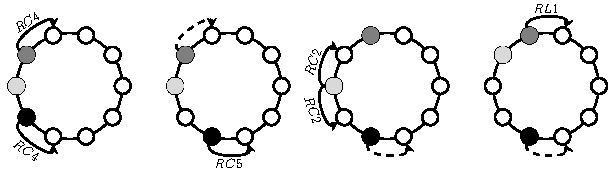
\includegraphics{figures/figCE1}
\label{fig:CE1} 
}\\\vspace{-2em}
\subfloat{
\centering
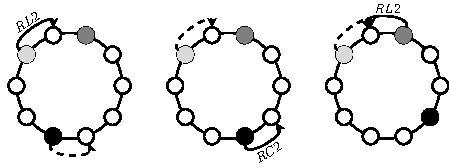
\includegraphics{figures/figCE2}
\label{fig:CE2} 
}
\caption{Counter-example.} 
\label{fig:CE} 
\end{figure*} 
 
In the starting configuration after the \textit{LC} phase of all
robots, the gray one and the black one have decided to move according
to the $RC4$ rule, and the light gray one to stay idle.  The black
robot moves, which produces the second configuration. Before the gray
robot could move, the black one performs its \textit{LC} phase and
according to the $RC5$ rules, it chooses to roll away from the two
other robots. The gray robot moves from the decision taken previously
and the third configuration is reached.  From this configuration the
light gray robot performs its \textit{LC} phase and chooses to move in
any direction (as the configuration has an axis of symmetry passing through
this robot). The scheduler makes it move toward the gray one.  From
the fourth configuration thus obtained, the gray robot had to move
according to rule $RL1$ after its \textit{LC} phase.  This movement
permits to obtain the fifth configuration, from where the light gray
robot chooses to move according to rule $RL2$.  We obtain the sixth
configuration thanks to the movement of the black robot (movement that
he had chosen in the second configuration).  From this configuration
the black robot chooses to move according to rule $RC4$, and the move
is performed.  In the last configuration the gray robot performs its
\textit{LC} phase and according to the $RL2$ rule, it chooses to move
toward the light gray one, on the same node where the light gray one
had chosen to go in the fifth configuration.  From there if these two
robots move, they collide.

In this counter-example, we can see that the collision is due to a sequence 
of movements made from outdated snapshots. Hence, we need to stop these 
movements.  We now
present a correction of the algorithm referred to as
\emph{Min-Algorithm-Corrected}. The change concerns the convergence
phase, the legitimate phase being unchanged.  More precisely, only
rule $RC5$ is modified to avoid collisions induced by the previous
rules, when movements computed on obsolete observations are taken into
account. The new $RC5$ rule is: 
$$RC5~~:: ~~(R_2, F_1, R_1, F_{n-4})~~\rightarrow~~r.\Back$$

Note that the moving robot has changed with respect to the old rule.
If this new rule is applied in the counter-example, then from the second
configuration, no movements from outdated snapshots can be made any
more since the $RC5$ rule requires a configuration where the light
gray and the black robots have stayed idle.

\begin{table}[!h] 
\centering 
\setlength{\tabcolsep}{5pt}
\begin{tabular}{|c|r|r|r|c|r|}
%{|n|k|States|Transitions|Memory|Model|Verif|Itérations|} 
\hline \textbf{n} &
\textbf{States} & \textbf{Transitions} & \textbf{Mem(kB)}&
\textbf{Time} \\ \hline 
10& ~1\, 581\, 961 & 6\, 090\, 209 & ~1\, 416\, 880 & 00: 06: 45 \\ \hline 
11& 1\, 926\, 385 & 7\, 421\, 315 & 1\, 568\, 748 & 00: 09: 09 \\ \hline 
13&2\, 716\, 637 & 10\, 476\, 317 & 2\, 252\, 600 & 00: 20: 46 \\ \hline 
14& 3\, 162\, 409 &12\, 307\, 905 & 2\, 560\, 724 & 00: 26: 54 \\ \hline 
16& 4\, 155\, 385 & 16\, 041\, 365& 2\, 772\, 188 & 00: 36: 22 \\ \hline 
\end{tabular} \caption{Model-checking of the
\emph{Min-Algorithm-Corrected}.} \label{tab: correct} \end{table}

Verification results (where correctness is obtained) are given in
Table~\ref{tab: correct} for several instances of $n$. All results
show a limited blow up, due to the fact that when the number $k=3$ of
robots is fixed, the maximal number of configurations (and of states) is
of order $n^3$.




		
		
		
		
% !TEX root = manuscrit.tex
	
Since this protocol is parameterized by the ring size $n$, 
model-checking does not permit to verify whether it is valid for all
values of $n$. Therefore, while automated verification was used to
prove the required properties for small values of $n$, we provide an
inductive proof to obtain the correctness for arbitrary values of $n$
in the asynchronous model.

%Synth:  we prove by induction that the mechanically generated algorithm is also correct for any ring size except when an impossibility result holds (that is, when the number of robots divides the ring size). Our method can be seen as a first step towards  ``correct by design'' actual robot protocol implementations. 


	\section{Correctness of the new algorithm }
\label{subsec:induction}  

We first prove point \emph{(c)}: the exploration is performed
by cycling within the legitimate configurations and point \emph{(b)}:
from all non-legitimate configurations a legitimate configuration is
reached.
%\todo{rappeler la reference de la def contenant les types (like $A$, $B$ or $L1$)}

\begin{definition}
\label{note:type}
We note $[Type^n(x, y, z), \ \varphi(x, y, z)]$ the set of
configurations such that $Type$ is the type of the configuration, $x$, $y$ and $z$ correspond to the number of free
nodes that isolate each robot from the other, and $\varphi(x, y, z)$ is
an additional constraint restricting the scope of values for $x, y, z$.
\end{definition}
Recall that $n = x+y+z+3$ remains constant, with $n\geq
10$. Constraints defining the type itself are omitted, for instance, 
$[B^n(x, y, x) \mid x\neq y \wedge $ $x> 0$ $\wedge \ n = y+2x+3]$ is
simply denoted by $[B^n(x, y, x)]$.



\begin{definition}
\label{note:state}
The tuple $(s_x, s_y, s_z, [\textit{Type}^n(x, y, z), \varphi(x, y, z)])$ denotes
the set $$\{(s_x, s_y, s_z, c) \mid c \in [\textit{Type}^n(x, y, z), 
\varphi(x, y, z)] \}$$ of system states, where $s_x$ (respectively $s_y$, 
$s_z$) is the local state of the robot positioned before the
$x$ (respectively $y$, $z$) free nodes.\\
For $w \in \{x, y, z\}$, state $s_w$ belongs to $\Front$, $\Back$, 
$\RLC$. For the sake of readability, we do not
represent $\textit{Idle}$ states, hence only scheduler choices about robots
that can move are seen.

For a set $P$ of system states, we denote by $\mathcal{C}(P)$ the set
of configurations of $P$ and by $\mathcal{R}(P)$ the set of rules of
the algorithm that can be applied on $P$. For a rule $R \in
\mathcal{R}(P)$, we define: $$succ_{R}(P)=\{s' \ | \ s \xrightarrow{R}
s' \textrm{ for some } s \in P\}$$ the set of states produced by
applying $R$ to states of $P$.
\end{definition}

%\todo{ref def 13}

An abstract view of the algorithm is shown in Figures~\ref{fig:all}
and~\ref{fig:lower} using these notations. Gray states are
initial states, more particularly the light gray ones are legitimate states.  Each
$\textit{Move}$ transition is guarded by a condition between brackets
and corresponds to the choice of the scheduler to let all robots
move. In the $\textit{Move}_{any}$ transition, the scheduler lets only
a single robot move.


\begin{figure}[htbp]
\centering
%\input{algomin.tex}
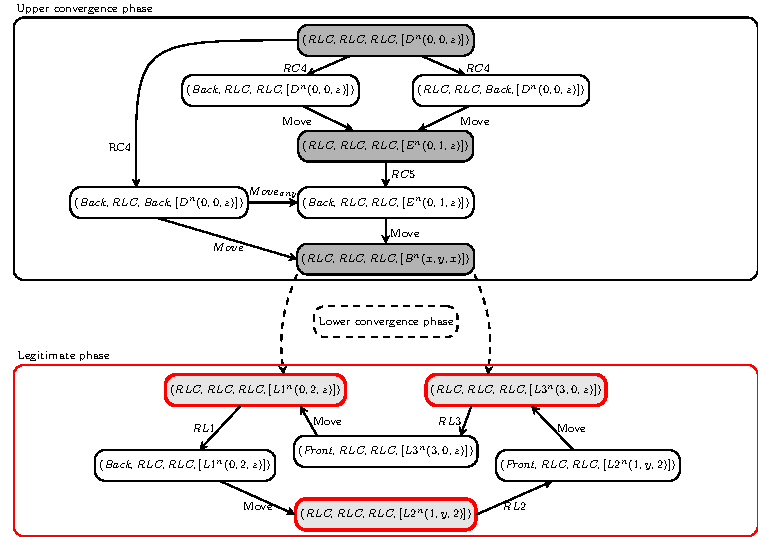
\includegraphics[scale=1.2]{figures/figALgoMin2}
\caption{Graph of Min-algorithm.}
 \label{fig:all}
\end{figure}

\begin{figure}[htbp]
\centering
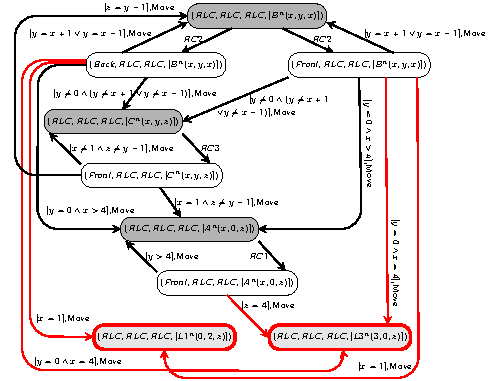
\includegraphics[scale=2]{figures/figlowerP}
\caption{Lower convergence phase.}
 \label{fig:lower}
\end{figure}

\subsubsection{Exploration from legitimate configurations}

We prove the following theorem:
\begin{theorem}
\label{th:legit}
From any legitimate configuration the ring (of size $n \geq 10$, 
co-prime with $3$) is perpetually explored.
\end{theorem}

\begin{figure}[bt] 
\centering
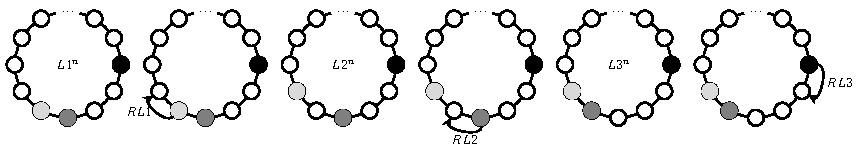
\includegraphics[scale=1]{figures/figLegit}
\caption{A step for the exploration.} 
\label{fig:Legit} 
\end{figure} 

The result holds if from a legitimate configuration ($L1, L2, L3$) only
legitimate configurations are reached, and if from any legitimate
configuration, an identical configuration is reached, where all
positions have been shifted $p$ times to the same direction, for any
$p\in\N$. In particular, when $p>0$ is a multiple of $n$, all robots
have visited all nodes.
These two properties are expressed by the following \textsf{LTL} formulas:\\

\begin{enumerate}[parsep=0cm, itemsep=0cm, topsep=0cm]
\item %\begin{lemma} 
\noindent \label{lem:GL}$\G \ (\mathbb{L} \Rightarrow \G \ \mathbb{L})$\\
%\end{lemma}
\item %\begin{lemma}
\label{lem:explor}$\forall i, m = 1, 2, 3$, $\forall j \in
  \{0, 1, \ldots, n-1\}$, $\forall p \in \mathbb{N}$, \\
  $\G (Lm \wedge r[j]=r_i \Rightarrow \F (Lm \wedge r[j+p]=r_i))$\\
%\end{lemma}
\end{enumerate}

  where $Lm$ is the predicate indicating that the configuration
  belongs to the corresponding set and $r[j]= r_i$ is the binary
  predicate giving the absolute position $j$ for robot $r_i$.

By construction and for all $n\geq 10$, the first formula is satisfied
since the only possible moves from $L1$, $L2$ and $L3$
for scheduled robots not staying idle are: \\\smallskip
\small{%%%%%%%%%%%%%%%%%%%%%%%%%%here%%%%%%%%%%%%%%%%%%%%%%%%%%%%%r                                                                                                                                                                                                                                                                                                                                                                                                                                                                                                                                                                                                                                                                                                                                                                                                                                                                                                                                                                                                                                                                                                                                                                                                                                                                                                                                                                                                                                                                                                     
\noindent
$succ_{RL1}~((\RLC, \RLC, \RLC, [L1^n(0, 2, n-5)]))$
$ = (\Back, \RLC, \RLC, [L1^n(0, 2, n-5)]), $\\ \smallskip
$ succ_{Move} (( \Back, \RLC, \RLC, [L1^n(0, 2, n-5)]))$ 
$= (\RLC, \RLC, \RLC, [L2^n(1, 2, n-6)]), $

\medskip \noindent
$succ_{RL2}~(( \RLC, \RLC, \RLC, [L2^n(1, 2, n-6)]))$
$ = (\RLC, \Front, \RLC, [L2^n(1, 2, n-6)]), $\\\smallskip
$succ_{Move} ((\RLC, \Front, \RLC, [L2^n(1, 2, n-6)]))$
$= (\RLC, \RLC, $ $\RLC, [L3^n(0, 3, n-6)]), $

\medskip \noindent
$succ_{RL3}~(( \RLC, \RLC, \RLC, [L3^n(0, 3, n-6)]))$
$ = (\RLC, \RLC, \Front, [L3^n(0, 3, n-6)]), $\\\smallskip
$succ_{Move} ((\RLC, \RLC, \Front, [L3^n(0, 3, n-6)]))$
$ = (\RLC, \RLC, \RLC, [L1^n(0, 2, n-5)]).$\\}

As mentioned previously, the second formula ensures the perpetual
exploration.  The proof is an easy induction over $p$, for an
arbitrary size $n$.

The base case for $p=1$:  $(Lk \wedge r[j]=r_i) \implies \F (Lk \wedge r[j+1]=r_i)$ 
results from chaining the three moves described above, 
as illustrated in Figure~\ref{fig:Legit}. For
the induction step, assume that the property holds for $p$.  This
implies: $$(Lk \wedge r[j]=r_i) \implies \F (Lk \wedge r[j+p]=r_i).$$
Setting $j'= j+p$ and
using the base case $(Lk \wedge r[j]=r_i) \implies \F (Lk \wedge r[j+1]=r_i)$, 
we obtain: $(Lk \wedge r[j']=r_i) \Rightarrow \F
(Lk \wedge r[j'+1]=r_i)$.\\Hence,  $(Lk \wedge r[j]=r_i) \Rightarrow \F (Lk
\wedge r[j+p+1] = r_i)$ 
and the property holds for $p+1$.


\subsubsection{Convergence from illegitimate configurations}

\begin{theorem}\label{th:conv}
  From any non legitimate configuration, a legitimate configuration is
  eventually reached (for a ring of size $n \geq 10$, co-prime with
  $3$).
\end{theorem}

To establish the convergence result, we associate with any subset $P$
of system states a tree $\T(P)$ rooted in $P$, with nodes the subsets
of states obtained by applying the rules of the algorithm.  Reaching a
set of successors in $\mathbb{L}$ without pending moves results in a
leaf.  More precisely:
\begin{definition}
\label{def:conv}
Given the set $\mathcal{R}$ of rules of the \emph{Min-Algorithm}, 
let $P_0$ be a subset of system states. The tree $\T(P_0)$ has
$P_0$ as root and for each node $P$:
\begin{itemize}
\item If $\mathcal{C}(P) \subseteq \mathbb{L}$ and for all $s \in P$, 
  $w \in \{x, y, z\}$, $s_w \notin \{\Front, Back \}$, then the node has
  no successor.
\item Otherwise the node $P$ has a successor $succ_{R}(P)$ for each $R
  \in \mathcal{R}(P)$.
\end{itemize}
\end{definition}

We now prove that for any set of states $P$ such that $\mathcal{C}(P)$
is contained in one of the non legitimate configurations types, the
tree $\T(P)$ is finite. This yields the desired convergence proof. If
for some $P$, the tree $\T(P)$ is infinite, then there exists an
infinite sequence of rules (on an infinite path of this tree) such
that for all successor sets $P'$ of $P$ along this sequence, either
$\mathcal{C}(P') \nsubseteq \mathbb{L}$ or there is some $s \in P'$
such that $s_w \in \{\Front, Back\}$ for some $w \in \{x, y, z\}$, 
meaning that the corresponding robot has a pending move.


To prove this result, we exhaustively verify the property for all
types $A^n$, $B^n$, $C^n$, $D^n$ or $E^n$, by inductive proofs, in
Lemmas~\ref{lemma:a} to~\ref{lemma:d} (where we assume $n \geq10$ and
$n$ co-prime with $3$). Note that  these lemmas must be proved in 
the order $A$, $C$, $B$, $E$ and $D$.
 Since $\mathbb{NL}^n = A^n \cup B^n \cup C^n
\cup D^n \cup E^n$ the result follows.
 

\begin{lemma}
\label{lemma:a}
The tree $\T(P)$ is finite for 
$P=(\RLC, \RLC, \RLC, 
[A^n(x, 0, z), 4 \leq x<z]).$
\end{lemma}
 
\begin{proof}
  The idea of the proof is as follows: recall that from an $A^n$
  configuration $(R_1, F_x, R_2, F_z)$ with $4 \leq x < z$, written
  $[A^n(x, 0, z), 4 \leq x<z]$, only one movement is feasible, leading to an
  $[L3^n(3, 0, z)]$ configuration if $x=4$ and to an $[A^n(x-1, 0, z+1)]$
  configuration otherwise.  Hence,  the number of free nodes in the $x$
  part decreases until an $L3$ configuration is reached.

  We first prove the property for an arbitrary $z$ when $x=4$ (base
  case). Then we prove the induction step on $x$.\\

%\begin{description}[parsep=0cm, itemsep=0cm, topsep=0cm]
\noindent \textbf{Base-case:} 
For $P=(\RLC, \RLC, \RLC, [A^n(4, 0, z)])$, with any $z \geq 6$,  the tree $\T(P)$ is finite
 with the moves:
\begin{center}
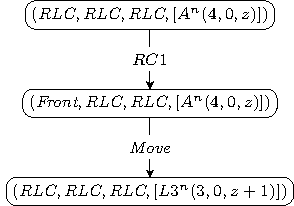
\includegraphics[scale=1]{figures/figAx4} 
\end{center}

\noindent \textbf{Induction step:} Assume that the tree
with root $P=(\RLC, \RLC, \RLC, [A^n(x, 0, z)])$, for any $z>x$ is
finite.
%when $n>10$ and $n, k$ are co-prime.
For $x+1 < z$, the moves are:
\begin{center}
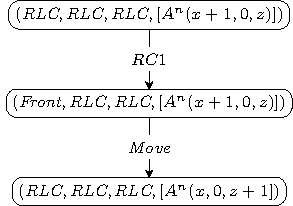
\includegraphics[scale=1]{figures/figA}
\end{center}
 they lead to $(\RLC, \RLC, \RLC, 
[A^n(x, 0, z+1])$ for which the tree is finite from the induction hypothesis. 
This ensures the desired result.
\end{proof}

\begin{lemma}
\label{lemma:c} The tree $\T(P)$ is finite for\\
$P=(\RLC, \RLC, \RLC, [C^n(x, y, z), 0<x<z<y])$
with $(x, z) \neq (1, 2).$
\end{lemma}

\begin{proof}
%A configuration $ c \in C^n$ is of the form: 
%$(R_1, F_x, R_1, F_y, R_1, F_z)$ with $0<x<z<y$.
  We first fix parameter $x$ and show that the tree for $P$ is
  finite, for any $y, z$ with $0<x<z<y$. Then we prove by induction
  that it holds for any $x$ using the first proof as base case.

%\subparagraph{}%x=1 pour tout z-y
\begin{description}[parsep=0cm, itemsep=0cm, topsep=0cm]
\item [{\bf Base-case}: x=1]
\end{description}  
\begin{itemize}[parsep=0cm, itemsep=0cm, topsep=0cm] 
\item %z-y=1->$B^n$ 
	If $z = y-1$, the tree is:
	\begin{center}
	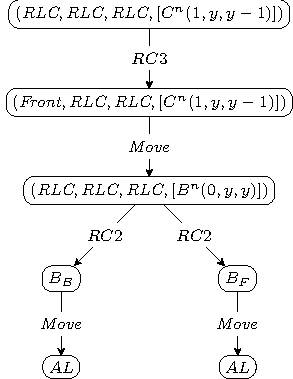
\includegraphics[scale=1]{figures/figCx12} 
	\end{center}
	where: \\
$ B_B = (\RLC, \RLC, \Back, [B^n(0, y, y)])$ and $ B_F = (\RLC, \RLC, \Front, [B^n(0, y, y)])$
and if $y=4$, $AL  = (\RLC, \RLC, \RLC, [L3^n(3, 0, 5)])$\\
otherwise $y > 4$, $AL = (\RLC, \RLC, \RLC, [A^n(y-1, 0, y+1)])$\\
Note that in both cases, the move from $B_B$ or $B_F$ leads to the same 
equivalence class of configurations: an $L3^n$ class when $y=4$ and 
an $A^n$ class otherwise. 
From Lemma~\ref{lemma:a}, the result holds for 
$x=1$ and $z = y-1$.

\item %y > 2 and z-y !=1->$A^n$
	If $2 < z < y-1$ (Recall that if $z=2$, since $x=1$, 
it is a $L2^n$ configuration), the moves are:\\
$succ_{RC3}~((\RLC, \RLC, \RLC, [C^n(1, y, z)]))$
$ = (\Front, \RLC, \RLC, [C^n(1, y, z)]), $\\
$ succ_{Move} (( \Front, \RLC, \RLC, [C^n(1, y, z)])$
$= (\RLC, \RLC, \RLC, [A^n(0, y, z+1)])$.\\
The last configuration is an $A^n$ configuration since $2<z<y-1$.
Similarly as above,  
%since the tree of root\\
%	$(\RLC, \RLC, \RLC, [A^n(x, 0, z)])$ is finite, 
the property results from Lemma~\ref{lemma:a}.
\end{itemize}
Finally, it results from the above cases that the tree
$\T(\RLC, \RLC, \RLC, [C^n(1, y, z)])$
 is finite for any $y, z$.


\begin{description}[parsep=0cm, itemsep=0cm, topsep=0cm]
\item[{\bf Induction step:} ] We now assume that the tree of root
  $(\RLC, \RLC, \RLC, [C^n(x, y, z)])$ is finite
  for any $y$, $z$, and prove that the same is true for 
  $\T(\RLC, \RLC, \RLC, [C^n(x+1, y, z)]$.
\end{description}  
\begin{itemize}[parsep=0cm, itemsep=0cm, topsep=0cm]
\item If $z=y-1$, the tree is%fait
	\begin{center}
	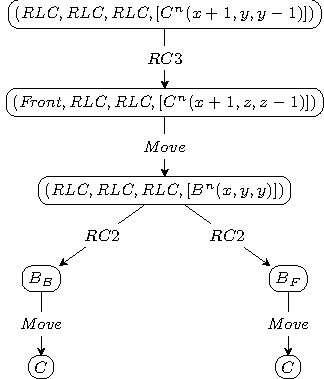
\includegraphics[scale=1]{figures/figCrec1} 
	\end{center}
	where\\
 	$\begin{array}{l c l}
B_B & = &(\RLC, \RLC, \Back, [B^n(x, y, y)])\\
B_F & = &(\RLC, \RLC, \Front, [B^n(x, y, y)]) \\
C & = &(\RLC, \RLC, \RLC, [C^n(x, y+1, y-1)])
\end{array}$\\
 	Thanks to the induction hypothesis, we can conclude that
  	the property holds in this case.
\item If $2 < z < y - 1$, applying the algorithm yields the movements: \\ 
$succ_{RC3}~((\RLC, \RLC, \RLC, [C^n(x+1, y, z)]))$
$ = (\Front, \RLC, \RLC, [C^n(x+1, y, z)]), $\\ 
$ succ_{Move} (( \Front, \RLC, \RLC, [C^n(x+1, y, z)])$ 
$= (\RLC, \RLC, \RLC, [C^n(x, y, z+1)])$.\\
The last configuration is a $C^n$ configuration since $2<z<y-1$, hence
the property holds from the induction hypothesis.
\end {itemize}
Finally all trees
$\T(\RLC, \RLC, \RLC, [C^n(x, y, z)])$ with
$0<x<z<y$ and $(x, z) \neq (1, 2)$ are finite.
% and thus from any $C^n$ configuration a legitimate configuration is
% finally reached, when $n \geq 10$ and $n, k$ are co-prime.
\end{proof}
%%%%%%%%%%%%%%%%%%%%%%%%%%%%%%%%%%%%%%%%%%%%%%%%%%%%%%
\begin{lemma}
\label{lemma:b}
The tree $\T(P)$ is finite for \\$P=(\RLC, \RLC, \RLC, [B^n(x, y, x), 
  x>0 \wedge x \neq y]).$
%$\forall c \in B^n, \texttt{conv}([B^n(x, y, y])=true$.

\end{lemma}
\begin{proof}
%For a simplification purpose this proof is done 
We handle two cases: $x>y$ and $x<y$.
% divisé en 2 un cas x < y et  x > y 

\noindent \textbf{Case $x>y$}:
%x <y pour tout y et ensuite pour tout x
  We first handle the subcases $y=0$ and $y=1$.
% a legitimate configuration
%  is eventually reached, then we show it for any $x, y$ such that
%  $x>y$.

%cas x=0 %y\geq 4
\begin{itemize}[parsep=0cm, itemsep=0cm, topsep=0cm]
\item When $y=0$, applying the algorithm yields the moves: \\
		\begin{center}
		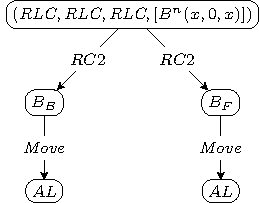
\includegraphics[scale=1]{figures/figBx0y4}
		\end{center}
	where \\
$\begin{array}{l c l}
	B_B & = &(\Back, \RLC, \RLC, [B^n(x, 0, x)])\\
	B_F & = &(\Front, \RLC, \RLC, [B^n(x, 0, x)]) 
\end{array}$\\
and if $x=4$, $AL =(\RLC, \RLC, \RLC, [L3^n(3, 0, 5)])$\\
otherwise $x>4$, $AL = (\RLC, \RLC, \RLC, [A^n(x-1, 0, x+1)])$\\
From $B^n$ configurations, where $y=0$, the moves lead to an $L3^n$ 
configurations when $x=4$, and to an $A^n$ configuration otherwise.
Hence,  from Lemma~\ref{lemma:a}, the property holds when $y=0$ for any $x$.
%cas x=1
\item When $y=1$, the tree representing the algorithm is the following:\\
		\begin{center}
		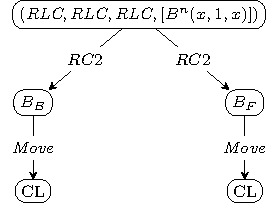
\includegraphics[scale=1]{figures/figBx1y3}
		\end{center}
		where\\
$\begin{array}{l c l}
	B_B & = &(\Back, \RLC, \RLC, [B^n(x, 1, x)])\\
	B_F & = &(\Front, \RLC, \RLC, [B^n(x, 1, x)])
\end{array}$\\
and if $x=3$, $CL =(\RLC, \RLC, \RLC, [L2^n(1, 4, 2)])$\\
otherwise $x>3$, $CL =(\RLC, \RLC, \RLC, [C^n(1, x+1, x-1)])$.\\
      Similarly as above there are two cases when $x=3$ or $x>3$.
      In the first case the moves reach $L2^n$ configurations, and in the
      second one to $C^n$ configurations.
      From Lemma~\ref{lemma:c}, the property holds when $y=1$ for any $x$.
\end{itemize}
	
\noindent
We now show the moves for any $x, y$ when $x>y>1$.  We need two
subcases when $x-1 = y$ and $x-1>y$.

\begin{itemize}[parsep=0cm, itemsep=0cm, topsep=0cm]
\item If $x-1=y$, the moves are:
	\begin{center}
	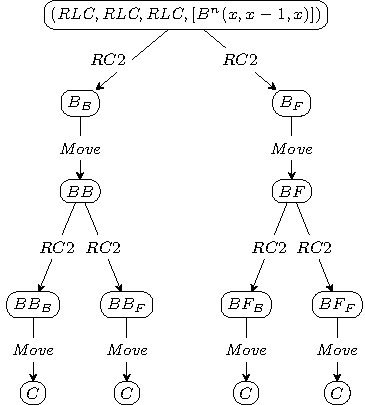
\includegraphics[scale=1]{figures/figBx+2y-1}
	\end{center}
	where\\
$\begin{array}{l c l}
	B_B & = &(\Back, \RLC, \RLC, [B^n(x, x-1, x)])\\
	B_F & = &(\Front, \RLC, \RLC, [B^n(x, x-1, x)])\\
	BB & = &(\RLC, \RLC, \RLC, [B^n(x+1, x-1, x-1)])\\
	BF & = &(\RLC, \RLC, \RLC, [B^n(x-1, x-1, x+1)])\\
		BB_B & = &(\RLC, \RLC, \Back, [B^n(x+1, x-1, x-1)])\\
		BB_F& = &(\RLC, \RLC, \Front, [B^n(x+1, x-1, x-1)])\\
		BF_B & = &(\RLC, \Back, \RLC, [B^n(x-1, x-1, x+1)])\\
		BF_F& = &(\RLC, \Front, \RLC, [B^n(x-1, x-1, x+1)])\\%%%
	C & = &(\RLC, \RLC, \RLC, [C^n(x-2, x+1, x)])\\
\end{array}$

\smallskip The property holds in this case, thanks to Lemma~\ref{lemma:c}.
\item If $x-1>y$, and $y>1$ the tree is:\\
	\begin{center}
	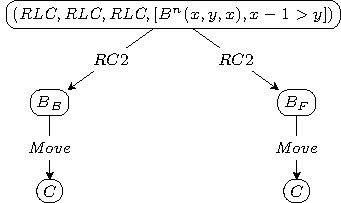
\includegraphics[scale=1]{figures/figBx+2y-1?}
	\end{center}
	where\\
		$\begin{array}{l c l}
	B_B & = &(\Back, \RLC, \RLC, [B^n(x, y, x)])\\
	B_F & = &(\Front, \RLC, \RLC, [B^n(x, y, x)])\\
	C & = &(\RLC, $ $\RLC, \RLC, [C^n(x+1, y, x-1)])	
		\end{array}$\\
and Lemma~\ref{lemma:c} entails the result. 
\end{itemize}
Hence,  $\T(\RLC, \RLC, \RLC, [B^n(x, y, x), x>y]))$ is finite.

%\medskip 
\noindent \textbf{Case $x<y$}: 
%x >y pour tout x et ensuite pour tout y
%We show that from any configuration of type $B$ 
%for any $x, y$ such that $x<y$ a legitimate configuration is eventually reached.
We handle two subcases when $y>x+1$ and $y=x+1$.

\begin{itemize}[parsep=0cm, itemsep=0cm, topsep=0cm] 
	\item If $x+1<y$, then the moves are:\\
		\begin{center}
		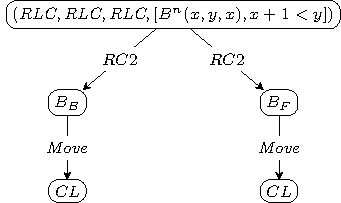
\includegraphics[scale=1]{figures/figBx1}
		\end{center}
	where\\
$\begin{array}{l c l}
B_B & = &(\Back, \RLC, \RLC, [B^n(x, y, x), x+1<y)])\\
B_F & = &(\Front, \RLC, \RLC, [B^n(x, y, x), x+1<y)
\end{array}$\\
and if $x=1$\\
$\begin{array}{l c l}
CL & = &(\RLC, $ $\RLC, \RLC, [L1^n(2, y, 0)])
\end{array}$\\
otherwise ($x>1$):\\
$\begin{array}{l c l}	
CL & = &(\RLC, \RLC, \RLC, [C^n(x-1, y, x+1)])
\end{array}$\\
When $x=1$ the moves lead to $L1^n$ configurations and 
to $C^n$ configurations otherwise.
Hence, again thanks to Lemma~\ref{lemma:c}, 
the property holds for any $x, y$ when $x+1<y$.

\smallskip
\item If $x+1=y$, the tree is:\\
		\begin{center}
		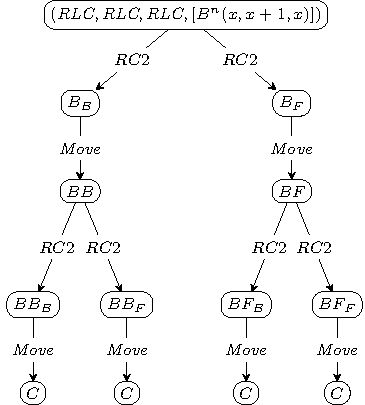
\includegraphics[scale=1]{figures/figBx+1y}
		\end{center}
	
		where\\
$\begin{array}{l c l}
B_B & = & (\Back, \RLC, \RLC, [B^n(x, x+1, x)])\\
B_F  & = & (\Front, \RLC, \RLC, [B^n(x, x+1, x)])\\
BB  & = & (\RLC, \RLC, \RLC, [B^n(x+1, x+1, x-1)])\\
BF & = &  (\RLC, \RLC, \RLC, [B^n(x-1, x+1, x+1)])\\
BB_B  & = & (\RLC, \Back, \RLC, [B^n(x+1, x+1, x-1)])\\
BB_F & = & (\RLC, \Front, \RLC, [B^n(x+1, x+1, x-1)])\\
BF_B & = & (\RLC, \RLC, \Back, [B^n(x-1, x+1, x+1)])\\
BF_F  & = & (\RLC, \RLC, \Front, [B^n(x-1, x+1, x+1)])\\
C & = & (\RLC, \RLC, \RLC, [C^n(x, x+2, x-1)])\\
\end{array}$\\

Since $\T(\RLC, \RLC, \RLC, [C^n(x, y, z)])$ is
finite (by Lemma~\ref{lemma:c}), the property holds.
\end{itemize}
Finally the trees
$\T(\RLC, \RLC, \RLC[B^n(x, y, x), x<y])$
are also finite, which concludes the proof.

%Hence,  $\T(\RLC, \RLC, \RLC, [B^n(x, y, x)])$ is finite.
\end{proof}

%Now the remaining lemmas are easier to prove.
\begin{lemma}
\label{lemma:e}
The tree $\T(P)$ is finite for $P=(\RLC, \RLC, \RLC, [E^n(0, 1, z)]).$
\end{lemma}

\begin{proof}
In the case of $E^n$ configurations, we have:
%\paragraph{Configurations of type $E$}
\begin{center}
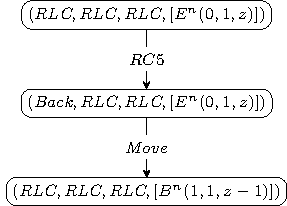
\includegraphics[scale=1]{figures/figE}
\end{center}
and the result holds thanks to Lemma~\ref{lemma:b}.
\end{proof}


\begin{lemma}
\label{lemma:d}
The tree $\T(P)$ is finite for $P=(\RLC, \RLC, \RLC, [D^n(0, 0, z)]).$
\end{lemma}
%\paragraph{Configurations of type $D$}

\begin{proof}
  From a $D^n$ configuration, it is also possible to schedule two
  robots with their respective planned moves. The various cases lead
  to either an $E^n$ configuration with or without a pending
  movement, or a $B^n$ configuration:\\
\begin{center}
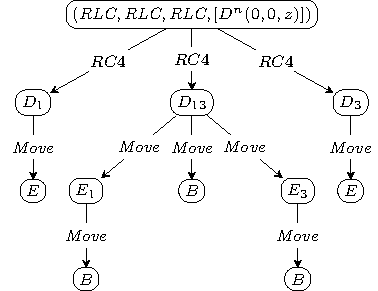
\includegraphics[scale=1]{figures/figD}%%%%%%%%%%%%%%%%%%%%%%%%%%%%%%%%%%%%%%%%%
\end{center}
	where\\
$\begin{array}{l c l}
D_1 & = &(\Back, \RLC, \RLC, [D^n(0, 0, z)])\\
D_{13} & = &(\Back, \RLC, \Back, [D^n(0, 0, z)])\\
D_3 & = &(\RLC, \RLC, \Back, [D^n(0, 0, z)])\\
E & = &(\RLC, \RLC, \RLC, [E^n(0, 1, z-1)])\\
E_1 & = &(\RLC, \RLC, \Back, [E^n(1, 0, z-1)])\\
E_3 & = &(\Back, \RLC, \RLC, [E^n(0, 1, z-1)])\\
B & = &(\RLC, \RLC, \RLC, [B^n(1, 1, z-2)])\\
\end{array}$\\
and the result holds from the previous lemmas~\ref{lemma:b} and~\ref{lemma:e}.
\end{proof}

%The proofs of the four other lemmas are similar and are given in
%Appendix.  
Together these lemmas imply Theorem~\ref{th:conv}. Finally, 
Theorems~\ref{th:legit} and~\ref{th:conv} give the result for
perpetual exploration. Moreover, since all reachable configurations
from any of the initial configurations are tower-free, the
\emph{Exclusivity} property follows (recall that the
\emph{No\_collision} property implies the \emph{No\_switch} property
in the asynchronous case as mentioned in
Section~\ref{subsub:perpexp}).  This concludes the correctness proof
of the algorithm.
	
			

%%%%%%%%%%%%%%%%%%%%%%%%%%%%%%%%%%%%%%%%%%%%%%%%%%
%%%%%%%%%%%%%%%%%%%%    Conclusion    %%%%%%%%%%%%%%%%%%%%%%
%%%%%%%%%%%%%%%%%%%%%%%%%%%%%%%%%%%%%%%%%%%%%%%%%%
%\section{Conclusion} We demonstrated the feasibility of formal
%verification through model-checking for mobile robot protocols in a
%discrete space. We verified two protocols for ring exploration. In the
%first case model checking helped in refining the correctness bounds of
%the protocol and in the second case it produced a counter-example,
%which permitted to correct the protocol. 
%We then proved the correctness of this protocol by induction.
%
%Our approach leads not only to find and correct bugs in the
%protocols (which is especially useful in the more challenging
%execution model ASYNC), but also relieves protocol designers from the
%burden of manually checking small instances of the problem, thus
%permitting them to concentrate on abstract configurations where some
%global invariants hold.


% !TEX root = manuscrit.tex

\part{Synthesis of mobile robot protocols}
\label{part:synth}

\chapter[Synchronous Synthesis]{Synthesis of synchronous mobile robot protocols}
\label{chap:synth}

In this chapter, we introduce the use of formal methods for automatic synthesis of autonomous mobile robot algorithms, in the discrete space model. As a case study, we consider the problem of gathering all robots at a particular position, not known beforehand. 
We propose an encoding of the gathering problem in a synchronous execution model as a reachability game, the players being the robot algorithm on one side and the scheduling adversary (that can also dynamically decide robot chirality at every activation) on the other side. Our encoding is general enough to encompass classical execution models for robots evolving on ring-shaped networks, including when several robots are located at the same node and when symmetric situations occur. Our encoding allow us to automatically generate an \emph{optimal} distributed algorithm, in the Fsync model, for three robots evolving on a fixed size ring. The optimality criterion refers to the number of robot moves that are necessary to actually achieve gathering.

\section {Gathering games}
\label{sec:jeux}
In this section we recall classical notions (from~\cite{DBLP:conf/dagstuhl/Mazala01}) related to two-player reachability games, \index{Two-player game} simply called games in the sequel. 

A game is composed of an \emph{arena} and \emph{winning conditions}.

\paragraph{Arena} \index{Arena}An arena for a two-player game is a graph $\arena=(V, E)$ in which the set of vertices
$V=V_p\uplus V_a$ is partitioned into $V_p$, the player locations, and $V_a$
the adversary locations. The set of edges $E\subseteq V\times V$ allows to
define the set of successors of some given vertex $v$, noted $vE=\{v'\in V\mid
(v, v')\in E\}$. %Sometimes the arena is such that $E\subseteq (V_p\times V_a) \cup (V_a\times V_p)$.
In the sequel, we only consider finite arenas.

\paragraph{Plays} \index{Play}To play on an arena, a token is positioned on an initial vertex. Then the token is moved by 
the players from one vertex to 
one of its successors. Each player can move the token only if it is on one of her own vertices. Formally, a play is
a path in the graph. Moreover, we only consider maximal plays:  a 
play is maximal if it is either infinite or finite such that the last vertex of the play has no successor
($\pi=v_0v_1\dots, v_n$, with $v_{n}E=\emptyset$).

\paragraph{Strategies}\index{Strategy}%des \sigma a la place des f...
A strategy for the player determines
to which position she will bring the token whenever it is her turn to play.
To do so, the player takes into account the history of the play, and the current
vertex.
Formally, a strategy for the player is a (partial) function
$\sigma:  V^*\cdot V_p \rightarrow V$ such that, for any sequence (representing the
current history) $w\in V^*$, any $v\in V_p$, $\sigma
(w\cdot v)\in vE$ (\ie the move is possible with respect to the arena). 
A strategy $\sigma$ is \emph{memoryless} if it does not depend on the history. Formally, it means
that for all
$w, w'\in V^*$, for all $v\in V_p$, $\sigma(w\cdot v) = \sigma(w'\cdot v)$. In that case, 
we may simply see the strategy as a mapping $\sigma: V_p\rightarrow V$.

Given a strategy $\sigma$ for the player, a play $\pi=v_0v_1\cdots \in V^\infty$
 is said to be \emph{$\sigma$-consistent} if for all $0<i<| \pi |$, if $v_{i-1}\in V_p$, then $v_i=\sigma
(v_0\cdots v_{i-1})$. Given an initial
vertex $v_{init}$, the \emph{outcome} of a strategy $\sigma$ is the set of plays starting in $v_{init}$
that are $\sigma$-consistent. Formally, given an arena $\arena=(V, E)$, an intial vertex $v_{init}$ and 
a strategy $\sigma: V^*V_p\rightarrow V$, we let $\Outcome(\arena, v_{init}, \sigma)=\{\pi \in V^\infty 
\mid v_0=v_{init}$ and  $\pi$ is a maximal play and is $\sigma$-consistent$\}$.

\paragraph{Winning conditions, winning plays, winning strategies}
 We define the \emph{winning condition} for the player as a subset of the plays $\Win \subseteq V^\infty$.
 Then, a play $\pi$ is \emph{winning} for the player if $\pi\in \Win$. In this work, we focus on the simple
 case of reachability games:  the winning condition is then expressed according to a subset of vertices $T\subseteq V$
 called the \emph{target} by $\Reach(T)=\{\pi=v_0v_1\cdots \in V^\infty\mid \pi$ is maximal and 
 $\exists i,  0\leq i < |\pi|:  v_i \in T\}$. This means that the player
 wins a play whenever the token is brought on a vertex belonging to the set $T$. Once it has happened, the play
 is winning, regardless of the following actions of the adversary.

Given an arena $\arena=(V, E)$, an initial vertex $v_{init}\in V$ and a
winning condition $\Win$, a
\emph{winning strategy} $\sigma$ for the player is a strategy such that
any $\sigma$-consistent play is winning. In other words, a strategy $\sigma$ is winning if
$\Outcome(\arena, v_{init}, \sigma) \subseteq Win$. The player wins the game $(\arena, v_{init}, \Win)$
if she has a winning strategy for $(\arena, v_{init}, \Win)$.
We say that $\sigma$ is winning on a subset $U \subseteq V$ if it is winning
starting from any vertex in $U$: 
$\Outcome(\arena, v, \sigma)\subseteq \Win$ for all $v\in U$.  A subset
$U \subseteq V$ of the vertices is \emph{winning} if there exists
a strategy $\sigma$ that is winning on $U$. The \emph{winning 
region} is the maximal winning set.

\paragraph{Solving a reachability game} \index{Reachability games}
Given an arena $\arena=(V, E)$, a subset $T\subseteq V$, one wants to 
determine the winning region $U\subseteq V$ of the player for $\Reach(T)$, 
and a strategy $\sigma: V^*V_p\rightarrow V$ 
for the player, that is winning on $U$.

\begin{example}
Figure~\ref{fig:synth} represents a reachability two-player game. 
\begin{figure}[htbp]
\centering 
\begin{tikzpicture} [thick, node distance= 6em, >=stealth, ->, scale=0.8, transform shape] 
\node[rectangle, draw, text centered](P1) {P1};
\node[rectangle, draw, text centered, left of =P1](P4){P4};
\node[circle, draw, text centered, above of = P1] (E1) []{O1};
\node[rectangle, draw, text centered, right of = E1](P2) {P2};
\node[circle, draw, text centered, above right= 1em and 4em of P1] (E3) []{O3};
\node[circle, draw, text centered, below right= 1em and 4em of P1] (E2) []{O2};
\node[rectangle, draw, text centered, above right = 1em and 4em of E2, fill=gray!60](P3) {P3};

\path (P1) edge[] (E1) 
         (P1) edge[] (P4)
	(E1) edge[] (P2) 
	(P2) edge[bend right] (E1) 
	(P1) edge[] (E2)
	(E1) edge [] (E3)
	(E2) edge[] node{} (P3)
	(P3) edge[] (E3)
	(E3) edge[] (P1)
	(P4) edge[loop above] (P4);
	
\end{tikzpicture} 
\caption{A two player game with a reachability objective.} 
\label{fig:synth}
\end{figure}
Player vertices are here represented by rectangles and adversary vertices by circles. 
The winning condition is $\Reach(\{P3\})$. 
From P2 the player has no winning strategy, since from O1 the adversary
can always bring the game back to P2, producing an infinite loop that never goes to the target. 
From P1 a (memoryless) winning strategy is to go to O2.
The winning region of the player is $\{P1, P3\}$.
\end{example}

We recall now a well-known result on reachability games~\cite{MartinBorelDeterminacy}: 
%stating that one does not need memory to win a reachability game: 
\begin{theorem} \label{th: memoryless}The winning region for the player in a reachability
game can be computed in linear time in the size of the arena. Moreover, from any location, the player
has a winning strategy if and only if she has a memoryless winning strategy.
\end{theorem}%The theorem obviously only make sense if the arena is finite (this is not require previously) -> in linear time:  according to the size of the arena







\section {Synthesis for synchronous robots}
		\subsection {Arena construction}
		\label{sub:synth}
We build an arena for a reachability game, such that the player has a winning strategy 
if and only if one can design an algorithm for synchronous robots to gather on a single node, 
starting from any configuration. We consider the arena $\Agather=(V_p\uplus V_a, E)$, 
where:  
\begin{itemize}
\item the set of player locations is $V_p= (\ObsClass)$, the set of equivalence classes of observations (see Definition~\ref{def:obs} in Chapter~\ref{chap:model}), 
\item the set of adversary locations 
is $V_a= \Obs \times \Actions^k$, with $\Actions=\{ \clockwise, \counterclockwise, \?, \still \}$  the set of actions as defined in~\ref{subsub:move}. 
\end{itemize}
The size of the arena is thus linear in $n$ and exponential in $k$.
The edge relation $E$ is detailed in the rest of the subsection and will ensure a strict alternation between the two players:  $E\subseteq (V_p\times V_a) \cup (V_a\times V_p)$.

\subsubsection{Edges from $V_p$ to $V_a$}
From a player location, representing an equivalence class of observations, 
the play continues on an adversary location memorizing the different movements
decided by each robot. Such a move is possible if, in a given equivalence class
of observations, the robots with the same view take the same decision. Recall that an algorithm 
$\mathcal{S}$ is given by a decision function (see Definition~\ref{def:decisionFunction} in Chapter~\ref{chap:model}).
\bigskip


We now define the edge relation from a player location to an adversary
location. For $v\in V_p$, recall that we can consider the canonical configuration $c_o$ for $o=\rep(v)$. 
Then $(v, v')\in E$ with $v'=\bigl (o, (a_1, \dots, a_k)\bigr )$ if and only if there exists 
a decision function $\partial$ such that $a_i=\dec(\view(r_i, c_o))$ for all $i$ in  $[1.. k]$.


\subsubsection{Edges from $V_a$ to $V_p$}
The moves of the adversary lead the game into the configuration of 
the system resulting from the application of the decisions of all robots. 
If a robot decides to move, but is disoriented, then the adversary
chooses the actual move (\clockwise{} or \counterclockwise). 
The next configuration is then determined by the actions chosen 
and the decisions taken by the adversary, defined as a $k$-tuple of movements
$m= (m_i)_{1\leq i \leq k} \in (\Actions \setminus \{\?\})^k$.

Let $r$ be a robot and let $c'$ be the configuration resulting from the move $m$ applied
to configuration $c$. We write $\obs(r, c') = \obs(r, c) \oplus m$ the corresponding 
observation. The next result states that the equivalence classes are consistent 
with equivalent movements of the robots. 
 \begin{proposition}
 \label{prop: bisim}
 Let $c \Cequiv c'$ be two equivalent configurations, and let $o$ and 
 $o'$ be observations of $c$ and $c'$ respectively.
 Then, for any move $m = (m_1, \dots, m_k)\in(\Actions \setminus \{\?\})^k$, there  
 exists $m' = (m'_1, \dots, m'_k)\in(\Actions \setminus \{\?\})^k$
  such that  $o\oplus m \equiv o'\oplus m'$.
 \end{proposition}
  \begin{proof}
 Let $c, c' \in \Config$ with
 $c'\Cequiv c$ and let $o, o' \in \Obs$ be observations of $c$ and $c'$ respectively. 
 For a  move $m=(m_i)_{1\leq i \leq k}\in (\Actions \setminus \{\?\})^k$ from $c$, 
 we define the move $m'$ that will represent the same decisions, on 
 configuration $c'$. Thanks to Proposition~\ref{prop:Oequ}, 
 we know that $o$ and $o'$ are in the same equivalence class for $\Oequiv$, hence 
if $o=\{(f_1, \cdots, f_k), (f_k, \cdots, f_1)\}$ then $o'=\{(f_i, \dots, f_k, f_1, \dots, f_{i-1}), (f_{i-1}, \dots, f_1, f_k, \dots, f_{i})\}$ 
for some $i$, $1\leq i\leq k$.
Now, ordering the two tuples of $o'$ in lexicographical order, we consider two cases.
If $(f_i, \dots, f_k, f_1, \dots, f_{i-1})$ is the smallest observation, then
 $m'_j=m_{(i+j-1)}$ for all $1\leq j\leq k$. Otherwise,  for all $1\leq j\leq k$:  
 $$m'_j= \begin{cases}
 \clockwise &\textrm{if }m_{i-j}=\counterclockwise\\
 \counterclockwise &\textrm{if }m_{i-j}=\clockwise\\
 \still &\textrm{if }m_{i-j}=\still
 \end{cases}$$
  We have $o\oplus m \equiv o'\oplus m'$.
 \end{proof}
 
We now define $v$-consistent moves where the adversary in some vertex $v$ resolves 
all the $\?$ actions by choosing in which directions disoriented robots will move.
\begin{definition}\label{def:vCo}
For a state $v=(o, (a_1, \dots, a_k))\in V_a$, a move $m = (m_1, \dots, m_k)\in(\Actions \setminus \{\?\})^k$
 is \emph{$v$-consistent} if:  
\begin{itemize}
\item for all $1\leq i\leq k$ such that $a_i\neq\disoriented$, $m_i=a_i$, 
\item for all $1\leq i\leq k$ such that $a_i=\disoriented$, $m_i\neq\still$.
\end{itemize}
\end{definition}


The edge relation from an adversary location 
to a player location is then defined by:  for $v=(o, (a_1, \dots, a_k))\in V_a$, and $v' \in V_p$, 
the edge $(v, v')$ belongs to $E$ if and only if there exists a $v$-consistent 
move m such that $v'=\equivclass{o\oplus m}$.

The Figure~\ref{fig:Agather} represents a part of the gathering arena for 4 robots on a ring of size 12.
\begin{figure}
\begin{tikzpicture} [thick, node distance= 14em, >=stealth, ->, scale=0.7, transform shape, text centered] 
\node[circle, minimum size =6.5em, draw, thick] (C){};
\node[rectangle, rounded corners=5pt, draw, below = 0.75em of C](W) {{$\equivclass{(-1, 1, 7, 1)}$}};
\foreach \i in {0, ..., 11}
\node[circle, minimum size =0.75em, draw, thick, fill=white]at(\i*30: 1.35)(W\i){};
\node[circle, minimum size =1em, draw, thick, fill=black]at(3*30: 1.35)(N1){};
\node[circle, minimum size =1em, draw, thick, fill=black]at(3*30: 1.7)(N2){};
\node[circle, minimum size =1em, draw, thick, fill=black]at(1*30: 1.35)(N3){};
\node[circle, minimum size =1em, draw, thick, fill=black]at(5*30: 1.35)(N4){};


\node[ellipse, draw, rounded corners=5pt, below  = 12.5 em of W](T1){(-1, 1, 7, 1), (D, D, I, I)};
\node[circle, minimum size =6.5em, draw, thick, below of =C](CT1){};
\foreach \i in {0, ..., 11}
\node[circle, minimum size =1em, draw, thick, fill=white, below of =W\i](T1\i){};
\node[circle, minimum size =1em, draw, thick, fill=black, below of =N1](N11){};
\node[circle, minimum size =1em, draw, thick, fill=black, below of =N2](N21){};
\node[circle, minimum size =1em, draw, thick, fill=black, below of =N3](N31){};
\node[circle, minimum size =1em, draw, thick, fill=black, below of =N4](N41){};


\node[ellipse, rounded corners=5pt, above = 11.25em of W, draw, node distance = 14em](T0){(-1, 1, 7, 1), (I, I, I, I)};
\node[circle, minimum size =6.5em, draw, thick, above of =C](CT0){};
\foreach \i in {0, ..., 11}
\node[circle, minimum size =1em, draw, thick, fill=white, above of =W\i](T0\i){};
\node[circle, minimum size =1em, draw, thick, fill=black, above of =N1](N10){};
\node[circle, minimum size =1em, draw, thick, fill=black, above of =N2](N20){};
\node[circle, minimum size =1em, draw, thick, fill=black, above of =N3](N30){};
\node[circle, minimum size =1em, draw, thick, fill=black, above of =N4](N40){};


\node[circle, minimum size =6.5em, draw, thick, above right = 3em and  7.75em of C](CT3){};
\foreach \i in {0, ..., 11}
\node[circle, minimum size =1em, draw, thick, fill=white, above right = 7em and  11.5em of W\i](T3\i){};
\node[circle, minimum size =1em, draw, thick, fill=black, above right = 7em and 11.5em of N1](N13){};
\node[circle, minimum size =1em, draw, thick, fill=black, above right = 7em and 11.5em of N2](N23){};
\node[circle, minimum size =1em, draw, thick, fill=black, above right = 7em and 11.5em of N3](N33){};
\node[circle, minimum size =1em, draw, thick, fill=black, above right = 7em and 11.5em of N4](N43){};
\node[ellipse, rounded corners=5pt, below = 0.25em of T39, draw](T3){(-1, 1, 7, 1), (D, D, F, F)};

\node[circle, minimum size =6.5em, draw, thick, below right = 3em and 7.75 em of C](CT4){};
\foreach \i in {0, ..., 11}
\node[circle, minimum size =1em, draw, thick, fill=white, below right = 7em and 11.5em of W\i](T4\i){};
\node[circle, minimum size =1em, draw, thick, fill=black, below right = 7em and 11.5em of N1](N14){};
\node[circle, minimum size =1em, draw, thick, fill=black, below right = 7em and 11.5em of N2](N24){};
\node[circle, minimum size =1em, draw, thick, fill=black, below right = 7em and 11.5em of N3](N34){};
\node[circle, minimum size =1em, draw, thick, fill=black, below right = 7em and 11.5em of N4](N44){};
\node[ellipse, rounded corners=5pt, below = 0.25em of T49, draw](T4){(-1, 1, 7, 1), (I, I, F, F)};


\node[circle, minimum size =6.5em, draw, thick, above left = 3em and 7.75 em of C](CT5){};
\foreach \i in {0, ..., 11}
\node[circle, minimum size =1em, draw, thick, fill=white, above left = 7em and 11.5em of W\i](T5\i){};
\node[circle, minimum size =1em, draw, thick, fill=black, above left = 7em and 11.5em of N1](N15){};
\node[circle, minimum size =1em, draw, thick, fill=black, above left = 7em and 11.5em of N2](N25){};
\node[circle, minimum size =1em, draw, thick, fill=black, above left = 7em and 11.5em of N3](N35){};
\node[circle, minimum size =1em, draw, thick, fill=black, above left = 7em and 11.5em of N4](N45){};
\node[ellipse, rounded corners=5pt, below = 0.25em of T59, draw](T5){(-1, 1, 7, 1), (D, D, B, B)};


\node[circle, minimum size =6.5em, draw, thick, below left = 3em and 7.75 em of C](CT6){};
\foreach \i in {0, ..., 11}
\node[circle, minimum size =1em, draw, thick, fill=white, below left = 7em and 11.5em of W\i](T6\i){};
\node[circle, minimum size =1em, draw, thick, fill=black, below left = 7em and 11.5em of N1](N16){};
\node[circle, minimum size =1em, draw, thick, fill=black, below left = 7em and 11.5em of N2](N26){};
\node[circle, minimum size =1em, draw, thick, fill=black, below left = 7em and 11.5em of N3](N36){};
\node[circle, minimum size =1em, draw, thick, fill=black, below left = 7em and 11.5em of N4](N46){};
\node[ellipse, rounded corners=5pt, below = 0.25em of T69, draw](T6){(-1, 1, 7, 1), (I, I, B, B)};

%suite de CT3
\node[circle, minimum size =6.5em, draw, thick, above right = 7.1em and  7.5em of CT3](CT3A){};
\foreach \i in {0, ..., 11}
\node[circle, minimum size =1em, draw, thick, fill=white, above right = 11em and  11.5em of T3\i](T3A\i){};
\node[circle, minimum size =1em, draw, thick, fill=black, above right = 11em and 11.5em of T32](N13A){};
\node[circle, minimum size =1em, draw, thick, fill=black, above right = 11em and 11.5em of T34](N23A){};
\node[circle, minimum size =1em, draw, thick, fill=black, above right = 12.5em and 10em of T34](N33A){};
\node[circle, minimum size =1em, draw, thick, fill=black, above right = 11.75em and 10.75em of T34](N43A){};
\node[rectangle, rounded corners=5pt, below = 0.25em of T3A9, draw](T3A){$\equivclass{(-1, -1, 1, 9)}$};
\node[circle, minimum size =6.5em, draw, thick, right = 5.75em of CT3](CT3B){};
\foreach \i in {0, ..., 11}
\node[circle, minimum size =1em, draw, thick, fill=white, right = 11.5em of T3\i](T3B\i){};
\node[circle, minimum size =1em, draw, thick, fill=black, right = 11.5em of T32](B1){};
\node[circle, minimum size =1em, draw, thick, fill=black, above right = 0em and 0em of B1](NB23){};
\node[circle, minimum size =1em, draw, thick, fill=black, right = 11.5em of T34](NB33){};
\node[circle, minimum size =1em, draw, thick, fill=black, above left = 0em and 0em of NB33](NB43){};
\node[rectangle, rounded corners=5pt, below = 0.25em of T3B9, draw](T3B){$\equivclass{(-1, 1, -1, 9)}$};


%suite de CT4
\node[circle, minimum size =6.5em, draw, thick, right = 5.75em of CT4](CT4bis){};
\foreach \i in {0, ..., 11}
\node[circle, minimum size =1em, draw, thick, fill=white, right = 11.5em of T4\i](T4B\i){};
\node[circle, minimum size =1em, draw, thick, fill=black, right = 11.5em of T42](TB42){};
\node[circle, minimum size =1em, draw, thick, fill=black, right = 11.5em of T43](TBB){};
\node[circle, minimum size =1em, draw, thick, fill=black, above = 0em of TBB](NB43){};
\node[circle, minimum size =1em, draw, thick, fill=black, right = 11.5em of T44](NB44){};
\node[rectangle, rounded corners=5pt, below = 0.25em of T4B9, draw](T4B){$\equivclass{(-1, 0, 9, 0)}$};

%suite de CT5
\node[circle, minimum size =6.5em, draw, thick, above left = 7.1em and  7.5em of CT5](CT5A){};
\foreach \i in {0, ..., 11}
\node[circle, minimum size =1em, draw, thick, fill=white, above left = 11em and  11.5em of T5\i](T5A\i){};
\node[circle, minimum size =1em, draw, thick, fill=black, above left = 11em and 11.5em of T50](N50A){};
\node[circle, minimum size =1em, draw, thick, fill=black, above left = 11em and 11.5em of T52](N52A){};
\node[circle, minimum size =1em, draw, thick, fill=black, above right = 0em and 0em of N52A](N52AA){};
\node[circle, minimum size =1em, draw, thick, fill=black, above left = 11em and 11.5em of T56](N56A){};
\node[rectangle, rounded corners=5pt, below = 0.25em of T5A9, draw](T5A){$\equivclass{(-1, 1, 5, 3)}$};
\node[circle, minimum size =6.5em, draw, thick, left = 5.75em of CT5](CT5B){};
\foreach \i in {0, ..., 11}
\node[circle, minimum size =1em, draw, thick, fill=white, left = 11.5em of T5\i](T5B\i){};
\node[circle, minimum size =1em, draw, thick, fill=black, left = 11.5em of T50](N50B){};
\node[circle, minimum size =1em, draw, thick, fill=black, left = 11.5em of T52](NB52){};
\node[circle, minimum size =1em, draw, thick, fill=black, left = 11.5em of T54](NB54){};
\node[circle, minimum size =1em, draw, thick, fill=black, left = 11.5em of T56](NB56){};
\node[rectangle, rounded corners=5pt, below = 0.25em of T5B9, draw](T5B){$\equivclass{(1, 1, 1, 5)}$};


%suite de CT6
\node[circle, minimum size =6.5em, draw, thick, left = 5.75em of CT6](CT6bis){};
\foreach \i in {0, ..., 11}
\node[circle, minimum size =1em, draw, thick, fill=white, left = 11.5em of T6\i](T6B\i){};
\node[circle, minimum size =1em, draw, thick, fill=black, left = 11.5em of N26](TB26){};
\node[circle, minimum size =1em, draw, thick, fill=black, left = 11.5em of N16](NB16){};
\node[circle, minimum size =1em, draw, thick, fill=black, left = 11.5em of T60](NB60){};
\node[circle, minimum size =1em, draw, thick, fill=black, left = 11.5em of T66](NB66){};
\node[rectangle, rounded corners=5pt, below = 0.25em of T6B9, draw](T6B){$\equivclass{(-1, 2, 5, 2)}$};

%suite de T1
\node[circle, minimum size =6.5em, draw, thick, below right = 3em and 7.75 em of CT1](CT1A){};
\foreach \i in {0, ..., 11}
\node[circle, minimum size =1em, draw, thick, fill=white, below right = 7em and 11.5em of T1\i](T1A\i){};
\node[circle, minimum size =1em, draw, thick, fill=black, below right = 7em and 11.5em of T11](T11A){};
\node[circle, minimum size =1em, draw, thick, fill=black, below right = 7em and 11.5em of T12](T12A){};
\node[circle, minimum size =1em, draw, thick, fill=black, below right = 7em and 11.5em of T14](T14A){};
\node[circle, minimum size =1em, draw, thick, fill=black, below right = 7em and 11.5em of T15](T15A){};
\node[rectangle, rounded corners=5pt, below = 0.25em of T1A9, draw](T1A){$\equivclass{(0, 1, 0, 7)}$};

\node[circle, minimum size =6.5em, draw, thick, below left = 3em and 7.75 em of CT1](CT1B){};
\foreach \i in {0, ..., 11}
\node[circle, minimum size =1em, draw, thick, fill=white, below left = 7em and 11.5em of T1\i](T1B\i){};
\node[circle, minimum size =1em, draw, thick, fill=black, below left = 7em and 11.5em of T11](T11B){};
\node[circle, minimum size =1em, draw, thick, fill=black, below left = 7em and 11.5em of T14](T12B){};
\node[circle, minimum size =1em, draw, thick, fill=black, above left = 0em and 0em of T12B](T12BB){};
\node[circle, minimum size =1em, draw, thick, fill=black, below left = 7em and 11.5em of T15](T15B){};
\node[rectangle, rounded corners=5pt, below = 0.25em of T1B9, draw](T1B){$\equivclass{(-1, 0, 7, 2)}$};
	
	
\path		(N2.north) edge[] (T0.south)
	 	(W.south) edge[] (N21.north)
		(W2) edge[] (T37)
		(W11) edge[] (T44)
		(W4) edge[] (T511)
		(W7) edge[] (T62)
		(T66) edge[] (T6B0)
		(T56) edge[] (T5B0)
		(T54) edge[] (T5A11)
		(T30) edge[] (T3B6)
		(T32) edge[] (T3A7)
		(T40) edge[] (T4B6)
		(T17) edge[] (T1B2)
		(T111) edge[] (T1A4)
		;%[bend right=75, looseness=1.5] (N2.north east);

\end{tikzpicture} 
\caption{A part of the gathering arena for 4 robots in a 12 nodes ring.} 
\label{fig:Agather}
\end{figure}


\bigskip

In this context, gathering can be reformulated as follows: \\
Let $v_T=\equivclass{(-1, \cdots, -1, n-1), (n-1, -1, \cdots, -1)}\in V_p$ 
be the equivalence class 
of all configurations corresponding to all robots positioned on a single node.
For the game on $\Agather$ with winning condition $\Reach(\{v_T\})$, the winning region corresponds
 exactly to the set of configurations from which robots can achieve the gathering. 
 
We must show now that solving this reachability game 
amounts to automatically synthesizing a deterministic algorithm achieving the gathering for this system.
Let $\mathcal{S}$ be an algorithm given by its decision function $\dec_\mathcal{S}$.
The notion of consistency is adapted to $\mathcal{S}$ as follows:  
for a configuration $c\in\Config$ and a corresponding observation $o\in \Obs$, 
$m \in (\Actions \setminus \{\?\})^k$ is a $(\mathcal{S}, c)$-consistent move 
if it is a $v$-consistent move for $v=(o, (a_1, \dots, a_k))$ with 
$a_i=\dec_\mathcal{S}(\view(r_i, c))$, $1\leq i \leq k$. We denote by $M(\mathcal{S}, c)$ the set of all $(\mathcal{S}, c)$-consistent moves.\\
 Let $c, c'$ be two configurations, and let $o$ and $o'$ be observations such that $o = \obs(r, c)$ and $o'=\obs(r, c')$
 for some robot $r$. We denote by $c\xrightarrow{m} c'$ 
 the application to configuration $c$ of the move $m$, where $m$ is $(\mathcal{S}, c)$-consistent,  
 leading to configuration $c'$, defined by:  $o' = o \oplus m$.
 
For a configuration $c$, we note $\suc(\mathcal{S}, c)$ 
the set of configurations produced by applying $M(\mathcal{S}, c)$ on $c$, 
more formally:    $$\suc(\mathcal{S}, c) = \{ c' \mid \exists m \in M(\mathcal{S}, c) \st c\xrightarrow{m} c' \}.$$
Proposition~\ref{prop: bisim} implies that, for two equivalent configurations $c\Cequiv c'$, 
$\suc(\mathcal{S}, c)  = \suc(\mathcal{S}, c')$.

The next result gives the correspondence between algorithms and winning strategies in the reachability game.
\begin{theorem}\label{th: correctness}
There exists an algorithm which achieves gathering if and only if there exists a memoryless winning strategy 
for the reachability game $\Agather$ with winning condition $\Reach(\{v_T\})$.
\end{theorem}

\begin{proof}
We first show that if some algorithm $\mathcal{S}$ achieves gathering 
then we can build a winning strategy $\sigma: V_p\rightarrow V_a$. 
Conversely we show that given a winning region and a memoryless strategy, one can 
define a unique algorithm for the robots.

From $\mathcal{S}$ we construct the memoryless strategy $\sigma$ defined for any 
$v \in V_p$ by:  $$\sigma(v) = 
(rep(v), (a_1, \dots, a_k)) \textrm{ with } a_i=\dec_\mathcal{S}(\view(r_i, c_{rep(v)})), 1\leq i \leq k.$$
We now have to prove that if $\mathcal{S}$ achieves the gathering then $\sigma$ is winning.
Our interest is on the plays in the $\Outcome$ of $\sigma$:  these plays are $\sigma$-consistent
and any edge $(v, v') \in V_a \times V_p$ in these plays results from a $v$-consistent move: 
For such an edge $(v, v')$, let $c$ be the configuration in $v$, with observation $o$, there exists a $v$-consistent 
move $m$ such that $v'= \equivclass{o'}$, with $o' = o \oplus m $. 
Since $m$ is also $(\mathcal{S}, c)$-consistent, then 
$c' \in \suc(\mathcal{S}, c)$ 
and thus, any configuration from which the algorithm ensures gathering is winning for the game.

Conversely, let $W$ be the winning region, and let $\sigma$ be a (memoryless, from 
Theorem~\ref{th: memoryless}) winning strategy. 
For a configuration $c \in \Config$, $o$ a corresponding observation, 
assume that the strategy is defined by:   $\sigma(\equivclass{o}) = 
(rep(\equivclass{o}), (a_1, \dots, a_k))$.  Then, we define a unique algorithm $\mathcal{S}$ 
by extracting the decision function underneath the strategy as follows:   
$\dec_\mathcal{S}(\view(r_i, c))= a_i$, for all robots $r_i \in \Rob$. 
%Thanks to our arena construction:   two robots on a same tower has the same view, 
%two symmetrical robots have the same view and disoriented robots have only two 
%possible actions:  $\?$ and $\Idle$.
We now show that this algorithm achieves gathering from any configuration $c$ such that its 
observation class $\equivclass{o}$ belongs to  $W$.
%The robots implementing $\mathcal{S}$ achieve the gathering from $c$ if
%for all $c' \in \suc(\mathcal{S}, c)$ the plays $\equivclass{\obs(r, c)} $ is f-consistent since f is a winning strategy. 
Let $c'$ be a configuration in $\suc(\mathcal{S}, c)$, then there exists a 
$(\mathcal{S}, c)$-consistent move $m \in M(\mathcal{S}, c)$ such that $c\xrightarrow{m} c' $. 
 %Since $m$ is also consistent with $f_\mathcal{S}$
  %such that $\obs(r, c) \oplus m = \obs(r, c')=o'$. 
 For all succession of configurations 
$c\xrightarrow{m} c'\xrightarrow{} \dots$ obtained by successive applications of the algorithm, 
we have a corresponding play %$(\equivclass{\obs(r, c)})v(\equivclass{o'})\dots$ 
that is $\sigma$-consistent, in the game. 
Since $\equivclass{o}$ is a winning position, the play is winning and $\mathcal{S}$
achieves gathering. 
\end{proof}

In the following subsection we explain in details how the robot moves have been implemented. 
%pas forcément à lire pour un reader ne voulant pas encoder nos robot moves 
In particular the  $o \oplus m$ notation is defined explicitely
 here.

%%%%%%%%%%%%%%%%%%%%%%%%%%%%%%%%
\subsection {Implementation details}
\label{subsec:implemSync}
%%%%%%%%%%%%%%%%%%%%%%%%%%%%%%%%

%\todo{ici on doit avoir les mouvements inverse car on est plus sur les mouvements 
%des robots mais sur les mouvements et leur efficience sur la configuration
%dans la partie asynchrone dire que ça doit être fait a chaque étape ...}

For efficiency reasons, our implementation does not handle configurations but only observations. 
More precisely we only work on the smallest $k$-tuple in $\mathcal{F}$ of an observation, 
from which we must recover the relevant information to perform robot moves.
Recall (from Subsection \ref{subsubsec:obs}) that from an observation class
$\obs \in \ObsClass$, we extract an observation $rep(\obs) = o =
\{F, \tilde{F}\}$ with $F=(f_1, \dots, f_k)$ in $\mathcal{F}$ minimal among all tuples in $\obs$.
We associate with $o$ a canonical configuration 
$c_o$ defined by $c_o(r_1)=0$, $c_o(r_2)=f_1+1, \dots, 
 c_o(r_k) = \Sigma_{i=1}^k f_i \plusN k$ 
where the robot $r_i$ is at distance $f_i$ of robot $r_{i \plusK 1}$.  

 Recall that a robot movement in $\Front, \Back, \Idle$ is given according to 
 the robot minimal view (see the paragraph~\ref{subsub:move}). 
 When a robot $r_i$ moves, it modifies the distances $f_i$ and $f_{i-1}$ 
 (increasing one of these two distances by one, and  decreasing by one 
 the other). Formally, the effect on an observation of a  configuration, 
 of any movement $m_i$ of robot $r_i$ can be described by a mapping 
 $\varepsilon:   \{1, \ldots, k\} \times \{\Front, \Back, \Idle\} \times F \to \{-1, 0, 1\}^k$.
 This mapping denotes the translated moves 
 that permit to apply real movements on the observations class and 
 is defined by:   \begin{itemize}
 \item If $\view^{\min\_r} \circlearrowright ^m F$ for some $m$ then
		$\varepsilon(i, \Back, F)$ = $\varepsilon_{i, \Back}$, 
		and $\varepsilon(i, \Front, F)$ = $\varepsilon_{i, \Front}$.
\item If there exists $F'$ in $\mathcal{F}$ such that $\view^{\min\_r} \sim F'$ 
and $F' \circlearrowright ^m F$ for some $m$ then
		$\varepsilon(i, \Back, F)$ = $\varepsilon_{i, \Front}$, 
		and $\varepsilon(i, \Front, F)$ = $\varepsilon_{i, \Back}$, 
\item and $\varepsilon(i, \Idle, F) = 0^k$.
 \end{itemize}
where $\varepsilon_{i, \Back}$ and $\varepsilon_{i, \Front}$ are defined by:  \\
\begin{minipage}{0.2\textwidth}
\end{minipage}
\hfill\begin{minipage}{0.4\textwidth}
$\varepsilon_{i, \Back}= (\varepsilon_{i, h})_{1\leq h\leq k}$ with:  
\begin{itemize}[noitemsep, topsep=0pt, parsep=0pt, partopsep=0pt]
\item $\varepsilon_{i, i-1}=-1$, 
\item $\varepsilon_{i, i}=1$, 
\item $\varepsilon_{i, h}=0$ for $h \notin \{i-1, i\}$.
\end{itemize}
\end{minipage}
\qquad
\begin{minipage}{0.4\textwidth}
$\varepsilon_{i, \Front}= (\varepsilon_{i, h})_{1\leq h\leq k}$ with:  
\begin{itemize}[noitemsep, topsep=0pt, parsep=0pt, partopsep=0pt]
\item $\varepsilon_{i, i}=-1$, 
\item $\varepsilon_{i, i-1}=1$, 
\item $\varepsilon_{i, h}=0$ for $h \notin \{i-1, i\}$. 
\end{itemize}
\end{minipage}

\medskip
The idea is to add (in an element-by-element fashion) the current observation
to all the vectors representing the movements of the robots to obtain the next 
configuration. However, when the movements of two adjacent robots imply 
that they switch their positions in the ring, some absurd values (-2 or -3) 
may appear in the obtained configuration, if the sum is naively performed, 
so a careful treatment of these particular cases must be done. To obtain 
the correct configuration, one should recall that robots are anonymous, 
hence if two robots switch their positions, it has the same effect as if none 
of them has moved. Also, if in a tower, some robots want to move $\clockwise$, 
and the others want to move $\counterclockwise$, the exact robots that will move 
are of no importance:  only the number of robots that move in each direction is important. 
We will then reorganize the movements between the robots, in order
 to keep correct values in our configurations:  
 \begin{itemize}
 \item in a tower, we assume that the robots that move $\counterclockwise$
	 always are the bottom ones, and robots that move $\clockwise$ are the 
	 top ones, 
\item when a robot moves $\clockwise$ and joins a tower, we assume that 
	 it is placed at the bottom of the tower,  
\item and when it moves $\counterclockwise$ and joins a tower, it is 
 placed at the top of the tower. 
 \end{itemize}
 These conventions ensure that when adding the configuration  and the different
 movements, we obtain correct values.
  
 We define $\PosTower(F)$, a set that contains all towers, encoded by the identities of the first and the last robot in it:  
 $$\PosTower(F)=\{(i, j)\mid f_{i-1} \neq -1, f_j\neq -1\textrm{ and }\forall h, i\leq h< j, f_h=-1\}$$
 We then define
$$\Pos(F)=\PosTower(F) 
 \cup\{(i, i)\mid 1\leq i\leq k, f_i \neq -1 \textrm{ and } \ f_{i-1} \neq -1 \}$$ 
 that contains all the towers, and the identities of all the other robots (not part of a tower).
 
 We first reorganize the movements of the robots in the towers such that 
 robot moving to the $\Front$ are the top ones and robots moving to 
 the $\Back$ are the bottom ones.
 Given a move $(m_i)_{1\leq i \leq k}$ in $(\Actions \setminus \{\?\})^k$, and a tower $(i, j)\in\Pos(F)$, 
 let $N^\clockwise_{(i, j)}$ be the number of robots with $\clockwise$ movement in this tower, 
 defined by $$N^\clockwise_{(i, j)}=|\{\varepsilon_{\ell, \Front} \mid i\leq \ell \leq j\}|$$ and let  
$N^\counterclockwise_{(i, j)}$ be the number of robots that go $\counterclockwise$ in this tower, defined by:  
$$N^\counterclockwise_{(i, j)}=|\{\varepsilon_{\ell, \Back} \mid i\leq \ell \leq j\}|.$$ 
The modified movement of robot $\ell$ denoted by $\varepsilon'_\ell$ is then defined by:  
\begin{itemize}
 \item if $\ell$ is part of tower $(i, j)\in\PosTower(F)$, then $\varepsilon'_\ell=\varepsilon_{\ell, \counterclockwise}$, if $i\leq \ell \leq \bigl(N_{(i, j)}^\counterclockwise +i-1\bigr)$
 \item if $\ell$ is part of tower $(i, j)\in\PosTower(F)$, then $\varepsilon'_\ell = \varepsilon_{\ell, \clockwise}$ if $\bigl(N_{(i, j)}^\counterclockwise +i\bigr)\leq \ell \leq j$. 
 \item For all other robots $\varepsilon'_\ell=\varepsilon_\ell$. 
 \end{itemize}
 
 Now, we modify the $\varepsilon$ vectors  in order to delete pointless moves, corresponding to robots switching positions. 
 Let $(i, j)\in\Pos(F)$ be the element of $\Pos(F)$ considered and let $\varepsilon'$ be the current $k$-tuple of $k$-vectors
 encoding the moves. 
 \begin{itemize}
\item If $f_j\neq 0$, $\varepsilon''_\ell=\varepsilon'_\ell$ (there is no robot in the neighboring node in the clockwise direction). 
\item Otherwise, let $s \in [1..k]$ such that $(j+1, s)\in\Pos(F)$ (note that if $s=j+1$, there is only one single robot on the neighboring node). 
 \begin{itemize}
 \item If $N^{\clockwise}_{(i, j)}\geq N^{\counterclockwise}_{(j+1, s)}$, then 
 \begin{itemize}
 \item $\varepsilon''_\ell = \varepsilon_{\ell, \clockwise}$ for all $ j-N^\clockwise_{(i, j)}+N^\counterclockwise_{(j+1, s)}+1\leq \ell \leq j$, 
 \item $\varepsilon''_\ell=\varepsilon_{\ell, \Idle} $ for all $
 	\left.
  		\begin{array}{l}
    			 j-N^\clockwise_{(i, j)} +1 \leq \ell \leq j-N^\clockwise_{(i, j)}+  N^\counterclockwise_{(j+1, s)} \\
    			j+1 \leq \ell \leq j+N^\counterclockwise_{(j+1, s)} \\
  \end{array}
\right.$
 \item and $\varepsilon''_\ell=\varepsilon'_\ell$  for all other  $\ell$.
 \end{itemize}
 \item If $N^{\clockwise}_{(i, j)}< N^{\counterclockwise}_{(j+1, s)}$, then the modification is symmetrical. 
 \end{itemize}
 \end{itemize}
 When all the elements of $\Pos(F)$ have been visited, we obtain a tuple $(\varepsilon''_\ell)_{1\leq \ell \leq k}$.
 
 \begin{proposition}
%For all observations $o \in\Obs$, for all tuples $(m_i)_{1\leq i\leq k}$, $o+\Sum{i=1}{k} \varepsilon^f_i\in \Obs$, \\
%where $(\varepsilon^f_i)_{1\leq i\leq k}$ has been obtained as described above.
Given an observation class $\equivclass{o}$ and a tuple $m=(m_i)_{1\leq i \leq k}$ of movements 
 in $(\Actions \setminus \{\?\})^k$, the successor $\equivclass{o \oplus m}$ is obtained from $\rep(\equivclass{o})=\{F, \tilde{F}\}$ 
 as the class of $o' =\{F', \tilde{F'}\}$ where $F'= F+\sum_{i=1}^{k} \varepsilon''_i$, and $(\varepsilon''_i)_{1\leq i\leq k}$ has been 
 obtained as described above.
 \end{proposition}
 
 \begin{proof}
 Let $o \in \Obs$ with $\rep(\equivclass{o})=\{F, \tilde{F}\}$,  $F=(f_1, \dots, f_k)$, and let $m=(m_i)_{1\leq i \leq k}$ be a move. 
  For all $1\leq i\leq k$, if $f_i=0$, then if the robot $i$ wants to move in the direction of $i+1$, 
  and the robot  $i+1$ wants to move in the direction of $i$, 
  then by our construction, $\varepsilon''_i=\varepsilon_{i, \Idle}$ and $\varepsilon''_{i+1}=\varepsilon_{i+1, \Idle}$, 
  and the resulting distance will stay 0. 
  For all other decisions of the robots, the distance obtained will be positive. 
  If $f_i=-1$, by the reorganization of the robots on a tower, it is impossible
 that robot $i$ wants to move in the clockwise direction and that the robot $i+1$
  wants to move in the counterclockwise direction. Hence, the distance obtained
 is never less than $-1$. In all other cases, the obtained distance is necessarily positive.
 \end{proof} 
 

%%%%%%%%%%%%%%%%%%%%%%%%%%%%%%
		\section {Results of synthesis}
%%%%%%%%%%%%%%%%%%%%%%%%%%%%%%
In the case of a system with three robots, there are $6$ distinct types of configuration classes:   
\begin{itemize}
	\item The 3-robots tower configuration, which is the configuration to reach, 
	where observations are in the observations class
	$\equivclass{\{(-1, -1, n-1), (n-1, -1, -1)\}}$. From this class of configuration  
	the arena leads to $(\{(-1, -1, n-1), (n-1, -1, -1)\}, (a_1, a_1, a_1))$ 
	with $a_1 \in\{\still, \disoriented\}$. 
	However, these edges are of no interest for us since the gathering property is verified.
	\item The disoriented tower is a configuration where there is an axis of symmetry 
	passing through a two robots tower and the third robot (it occurs only when $n$ is odd).
	Observation belongs to the classes:  
	$\equivclass{\{(-1, \frac{n}{2}-1, \frac{n}{2}-1), (\frac{n}{2}-1, \frac{n}{2}-1, -1)\}}$.  
	In this case, all robots are disoriented and thus the possible actions are:  
	 $(a_1, \overline{a_1}, a_2)$ with $a_1, a_2\in\{\still, \disoriented\}$.
	\item The remaining tower configurations are the ones with observations in the classes $\equivclass{\{(-1, f_2, f_3), (f_3, f_2, -1)\}}$, 
	with as representative $\{(-1, f_2, f_3), (f_3, f_2, -1)\}$ with $-1<f_2< f_3 \in \N$.
	The actions are of the form $(a_1, \overline{a_1}, a_2\}$ with $a_1, a_2\in\{\counterclockwise, \clockwise, \still\}$.
	\item The symmetrical configuration is a configuration where its observations are 
	in $\equivclass{\{(f_1, f_1, f_2), (f_2, f_1, f_1)\}}$ with $-1\neq f_1 \neq f_2$ and $-1 \neq f_{2}$.
	 Note that with $3$ robots there is an axis of symmetry that goes through an occupied node.
	 If $f_1 < f_2$, the edges lead to $(\{(f_1, f_1, f_2), (f_2, f_1, f_1)\}, (a_1, a_2, \overline{a_1})$ 
	 with $a_1\in\{\clockwise, \counterclockwise, \still\}$ and $a_2\in\{\still, \disoriented\}$, 
	otherwise (when $f_1>f_2$) edges lead to \\$(\{(f_2, f_1, f_1), (f_1, f_1, f_2)\}, (a_1, \overline{a_1}, a_2))$. 
%	with $a_1\in\{\clockwise, \counterclockwise, \still\}$ and $a_2\in\{\still, \disoriented\}$.
	\item The rigid configurations are all other configurations which do not fall into any of the above categories, 
	the outgoing edges go to $(\{(f_1, f_2, f_3), (f_3, f_2, f_1)\}, (a_1, a_2, a_3))$ with $-1 < f_1 < f_2 < f_3$
	and $a_1, a_2, a_3\in \{\clockwise, \counterclockwise, \still\}$. 
\end{itemize}

We implemented the arena for three robots and different ring sizes, 
in the game-solver tool \textsc{Uppaal Tiga}~\cite{UPPAAL-TIGA}, 
and we verified the impossibility of the gathering from periodic configurations.
On the other hand, the winning positions for the player are all vertices in $V_p$ corresponding to non periodic configurations. 

%The arena without the periodic class of configurations, is the graph such that all player vertices are winning. 
Moreover, recall that we look for optimal strategies, minimizing the number of robot moves achieving gathering. 
For this, we enrich the model by adding weights on edges:  each edge is weighted by the number of robots that move.
We are looking for a strategy on this graph that minimizes the sum of the weight, whatever the adversary does.
%a shortest path algorithm on this graph such that the player vertices and adversary vertices

\subsection{A synthesized algorithm}
\label{algo}
The strategies obtained for 3 robots on rings of size 9 and 10
 are depicted in the graphs of Figure~\ref{fig:Strat}.
 \begin{figure}[htbp]
\centering 
\subfloat[) Strategies for 3 robots on an 9-nodes ring.]{
\centering
\begin{tikzpicture} [thick, node distance= 8em, >=stealth, ->, scale=0.65, transform shape, text centered] 
\node[rectangle, rounded corners=5pt](W) {};%{$-1, -1, 8$};
\node[right of = W, node distance=6em](test){};
\node[circle, minimum size =4em, draw, thick](CW){};
\foreach \i in {0, ..., 8}
\node[circle, minimum size =0.75em, draw, thick, fill=white]at(10- \i*40: 0.8)(W\i){};
\node[circle, minimum size =1em, draw, thick, fill=black]at(10-7*40: 0.8)(N1){};
\node[circle, minimum size =1em, draw, thick, fill=black]at(10-7*40: 1.2)(N2){};
\node[circle, minimum size =1em, draw, thick, fill=black]at(10-7*40: 1.6)(N3){};


\node[rectangle, rounded corners=5pt, below of =W](T0){};%{$-1, 0, 7$};
\node[circle, minimum size =4em, draw, thick, below of =W](CT0){};
\foreach \i in {0, ..., 8}
\node[circle, minimum size =1em, draw, thick, fill=white, below of =W\i](T0\i){};
\node[circle, minimum size =1em, draw, thick, fill=black, below of =N1](N1){};
\node[circle, minimum size =1em, draw, thick, fill=black, below of =N2](N2){};
\node[circle, minimum size =1em, draw, thick, fill=black, below of =W8](N3){};

\path (T08.north east) edge[bend right=75, looseness=1.5] (N2.north east);
\node[right of =T08, node distance= 1em](i10){};
\node[above of =i10, node distance = 5em](i01){};
\path (i10) edge[very thick] (i01);

\node[rectangle, rounded corners=5pt, below of = T0](T1){};%{$-1, 1, 6$};
\node[circle, minimum size =4em, draw, thick, below of =T0](CT1){};
\foreach \i in {0, ..., 8}
\node[circle, minimum size =1em, draw, thick, fill=white, below of =T0\i](T1\i){};
\node[circle, minimum size =1em, draw, thick, fill=black, below of =N1](N1){};
\node[circle, minimum size =1em, draw, thick, fill=black, below of =N2](N2){};
\node[circle, minimum size =1em, draw, thick, fill=black, below of =T00](N3){};

\path (T10.east) edge[bend right=75, looseness=1.5] (T18.north east);
\node[below of =i10, node distance= 7em](i21){};
\node[above of =i21, node distance = 4em](i12){};
\path (i21) edge[very thick] (i12);

\node[rectangle, rounded corners=5pt, below of = T1](T2){};%{$-1, 2, 5$};
\node[circle, minimum size =4em, draw, thick, below of =T1](CT1){};
\foreach \i in {0, ..., 8}
\node[circle, minimum size =1em, draw, thick, fill=white, below of =T1\i](T2\i){};
\node[circle, minimum size =1em, draw, thick, fill=black, below of =N1](N1){};
\node[circle, minimum size =1em, draw, thick, fill=black, below of =N2](N2){};
\node[circle, minimum size =1em, draw, thick, fill=black, below of =T11](N3){};

\path (T21.east) edge[bend right=100, looseness=2] (T20.north east);
\node[right of =T28, node distance= 1em](i32){};
\node[above of =i32, node distance = 5em](i23){};
\path (i32) edge[very thick] (i23);


\node[rectangle, rounded corners=5pt, below of = T2](T3){};%{$-1, 3, 4$};
\node[circle, minimum size =4em, draw, thick, below of =T2](CT1){};
\foreach \i in {0, ..., 8}
\node[circle, minimum size =1em, draw, thick, fill=white, below of =T2\i](T3\i){};
\node[circle, minimum size =1em, draw, thick, fill=black, below of =N1](N1){};
\node[circle, minimum size =1em, draw, thick, fill=black, below of =N2](N2){};
\node[circle, minimum size =1em, draw, thick, fill=black, below of =T22](N3){};

\path (T32.south) edge[bend right=100, looseness=2] (T31.south east);
\node[right of =T38, node distance= 1em](i43){};
\node[above of =i43, node distance = 5em](i34){};
\path (i43) edge[very thick] (i34);

\node[rectangle, rounded corners=5pt, left of = T2, node distance = 8 em](R1){};%{$0, 1, 5$};
\node[circle, minimum size =4em, draw, thick, left of =T2, node distance = 8 em](CR1){};
\foreach \i in {0, ..., 8}
\node[circle, minimum size =1em, draw, thick, fill=white, left of =T2\i, node distance = 8 em](R1\i){};
\node[circle, minimum size =1em, draw, thick, fill=black, left of =T27, node distance = 8 em](N1){};
\node[circle, minimum size =1em, draw, thick, fill=black, left of =T26, node distance = 8 em](N2){};
\node[circle, minimum size =1em, draw, thick, fill=black, left of =T20, node distance = 8 em](N3){};

\path (N2.south) edge[bend right=100, looseness=2, blue, in=-110] (N1.south);
\path (N3.250) edge[bend left=100, looseness=2, green, in=120] (R18.230);
\node[above of =N1, node distance= 0.5em](R1W){};
\node[left of =T15, node distance = 1em](T1R){};
\path (R1W) edge[blue, very thick] (T1R);

\node[rectangle, rounded corners=5pt, below of = R1](R2){};%{$0, 2, 4$};
\node[circle, minimum size =4em, draw, thick, below of = R1](CR2){};
\foreach \i in {0, ..., 8}
\node[circle, minimum size =1em, draw, thick, fill=white, below of =R1\i](R2\i){};
\node[circle, minimum size =1em, draw, thick, fill=black, below of =R17](N1){};
\node[circle, minimum size =1em, draw, thick, fill=black, below of =R16](N2){};
\node[circle, minimum size =1em, draw, thick, fill=black, below of =R11](N3){};

\path (N2.250) edge[bend right=100, looseness=2, blue] (N1.south);
\path (N3.south west) edge[bend left=75, looseness=1.5, green] (R20.west);
\node[above of =N1, node distance= 0.5em](R1W){};
\node[left of =T25, node distance = 1em](T2R){};
\node[below of =R17, node distance = 4em] (RR){};
\path (R1W) edge[blue, very thick] (T2R)
	 (R1W) edge[green, very thick] (RR);

\node[rectangle, rounded corners=5pt, below of = R2 ](R12){};%{$1, 2, 3$};
\node[circle, minimum size =4em, draw, thick, below of =R2 ](CR12){};
\foreach \i in {0, ..., 8}
\node[circle, minimum size =1em, draw, thick, fill=white,  below of =R2\i](R12\i){};
\node[circle, minimum size =1em, draw, thick, fill=black, below of =R27 ](N1){};
\node[circle, minimum size =1em, draw, thick, fill=black, below of =R25 ](N2){};
\node[circle, minimum size =1em, draw, thick, fill=black, below of =R21 ](N3){};

\path (N2.south east) edge[bend right=100, looseness=2, blue, in = -90 ] (R126.south east);
\path (N3.160) edge[bend left=100, looseness=2, green, in = 90] (R120.west);
\node[above of =N1, node distance= 0.5em](RtW){};
\node[below of =R27, node distance = 4em] (RR){};
\path (RtW) edge[blue, very thick] (RR);

\node[rectangle, rounded corners=5pt, left of = T1, node distance = 16em](S0){};%{$0, 0, 6$};
\node[circle, minimum size =4em, draw, thick, left of =T1, node distance= 16em](CS0){};
\foreach \i in {0, ..., 8}
\node[circle, minimum size =1em, draw, thick, fill=white, left of =T1\i, node distance= 16em](S0\i){};
\node[circle, minimum size =1em, draw, thick, fill=black, left of =T17, node distance= 16em ](N1){};
\node[circle, minimum size =1em, draw, thick, fill=black, left of =T16, node distance= 16em ](N2){};
\node[circle, minimum size =1em, draw, thick, fill=black, left of =T18, node distance= 16em ](N3){};

\path (N2.west) edge[bend left=100, looseness=2, orange] (N1.100);
\path (N3.east) edge[bend right=100, looseness=2, orange] (N1.80);
\node[above of =S07, node distance= 1.5em](S0T){};
\node[left of = W5, node distance = 1em](TS0){};
\path (S0T.center) edge[orange, very thick] (TS0);
\node[above of = R17, node distance = 0.5em](RS){};
\node[right of = S02, node distance = 1em](SR){};
\path (RS) edge[green, very thick] (SR);

\node[rectangle, rounded corners=5pt, below of = S0, node distance= 16em](S1){};%{$1, 1, 4$};
\node[circle, minimum size =4em, draw, thick, below of =S0, node distance= 16em](CS1){};
\foreach \i in {0, ..., 8}
\node[circle, minimum size =1em, draw, thick, fill=white, below of =S0\i, node distance= 16em](S1\i){};
\node[circle, minimum size =1em, draw, thick, fill=black, below of =S07, node distance= 16em](N1){};
\node[circle, minimum size =1em, draw, thick, fill=black, below of =S05, node distance= 16em](N2){};
\node[circle, minimum size =1em, draw, thick, fill=black, below of =S00, node distance= 16em](N3){};

\path (N2.west) edge[bend left=100, looseness=2, orange] (S16.north);
\path (N3.east) edge[bend right=100, looseness=2, orange] (S18.north);
\node[above of =S17, node distance= 1em](S1S0){};
\node[below of = S07, node distance = 5em](S0S1){};
\path (S1S0) edge[orange, very thick] (S0S1);
\node[right of =S12, node distance = 1em](SR){};
\path (RtW) edge[green, very thick] (SR);

\node[rectangle, rounded corners=5pt, below of = S1 ](R3){};%{$0, 3, 3$};
\node[circle, minimum size =4em, draw, thick, below of =S1 ](CR3){};
\foreach \i in {0, ..., 8}
\node[circle, minimum size =1em, draw, thick, fill=white, below of =S1\i ](R3\i){};
\node[circle, minimum size =1em, draw, thick, fill=black, below of =S17 ](N1){};
\node[circle, minimum size =1em, draw, thick, fill=black, below of =S13 ](N2){};
\node[circle, minimum size =1em, draw, thick, fill=black, below of =S12 ](N3){};

\path (N1.north) edge[bend right=100, looseness=2, violet] (R36.north west);
\path (N1.north) edge[bend left=100, looseness=2, violet] (R38.north east);
\node[above of =R37, node distance= 1.25em](S3Rter){};
\node[left of = R23, node distance = 1em](RterS3){};
\path (S3Rter.center) edge[violet, very thick] (RterS3);


\node[rectangle, rounded corners=5pt, above of = S0, red, node distance= 16em](S2){};%{$2, 2, 2$};
\node[circle, minimum size =4em, draw, thick, above of =S0, red, node distance= 16em](CS2){};
\foreach \i in {0, ..., 8}
\node[circle, red, minimum size =1em, draw, thick, fill=white, above of =S0\i, node distance= 16em](S2\i){};
\node[circle, minimum size =1em, draw, thick, fill=red, above of =S07, node distance= 16em](N1){};
\node[circle, minimum size =1em, draw, thick, fill=red, above of =S04, node distance= 16em](N2){};
\node[circle, minimum size =1em, draw, thick, fill=red, above of =S01, node distance= 16em](N3){};
\end{tikzpicture} 
}\hspace{0.2em}%%%%%%%%%%%%%%%%%%%%%%%%%%%%%%%%
\subfloat[) Strategies for 3 robots on a ring of 10 nodes.]{
\centering
\begin{tikzpicture} [thick, node distance= 8em, >=stealth, ->, scale=0.6, transform shape, text centered] 
\node[rectangle, rounded corners=5pt](W) {};%{$-1, -1, 8$};
\node[circle, minimum size =4em, draw, thick](CW){};
\foreach \i in {0, ..., 9}
\node[circle, minimum size =0.75em, draw, thick, fill=white]at(20- \i*36: 0.8)(W\i){};
\node[circle, minimum size =1em, draw, thick, fill=black]at(20-8*36: 0.8)(N1){};
\node[circle, minimum size =1em, draw, thick, fill=black]at(20-8*36: 1.2)(N2){};
\node[circle, minimum size =1em, draw, thick, fill=black]at(20-8*36: 1.6)(N3){};


\node[rectangle, rounded corners=5pt, below of =W](T0){};%{$-1, 0, 7$};
\node[circle, minimum size =4em, draw, thick, below of =W](CT0){};
\foreach \i in {0, ..., 9}
\node[circle, minimum size =1em, draw, thick, fill=white, below of =W\i](T0\i){};
\node[circle, minimum size =1em, draw, thick, fill=black, below of =N1](N1){};
\node[circle, minimum size =1em, draw, thick, fill=black, below of =N2](N2){};
\node[circle, minimum size =1em, draw, thick, fill=black, below of =W9](N3){};

\path (N3.north east) edge[bend right=75, looseness=1.5] (N2.north east);
\node[right of =T09, node distance= 1em](i10){};
\node[above of =i10, node distance = 5em](i01){};
\path (i10) edge[very thick] (i01);

\node[rectangle, rounded corners=5pt, below of = T0](T1){};%{$-1, 1, 6$};
\node[circle, minimum size =4em, draw, thick, below of =T0](CT1){};
\foreach \i in {0, ..., 9}
\node[circle, minimum size =1em, draw, thick, fill=white, below of =T0\i](T1\i){};
\node[circle, minimum size =1em, draw, thick, fill=black, below of =N1](N1){};
\node[circle, minimum size =1em, draw, thick, fill=black, below of =N2](N2){};
\node[circle, minimum size =1em, draw, thick, fill=black, below of =T00](N3){};

\path (T10.east) edge[bend right=75, looseness=1.5] (T19.north east);
\node[below of =i10, node distance= 7em](i21){};
\node[above of =i21, node distance = 4em](i12){};
\path (i21) edge[very thick] (i12);

\node[rectangle, rounded corners=5pt, below of = T1](T2){};%{$-1, 2, 5$};
\node[circle, minimum size =4em, draw, thick, below of =T1](CT1){};
\foreach \i in {0, ..., 9}
\node[circle, minimum size =1em, draw, thick, fill=white, below of =T1\i](T2\i){};
\node[circle, minimum size =1em, draw, thick, fill=black, below of =N1](N1){};
\node[circle, minimum size =1em, draw, thick, fill=black, below of =N2](N2){};
\node[circle, minimum size =1em, draw, thick, fill=black, below of =T11](N3){};

\path (T21.east) edge[bend right=100, looseness=2] (T20.north east);
\node[right of =T29, node distance= 1em](i32){};
\node[above of =i32, node distance = 5em](i23){};
\path (i32) edge[very thick] (i23);

\node[rectangle, rounded corners=5pt, below of = T2](T3){};%{$-1, 3, 4$};
\node[circle, minimum size =4em, draw, thick, below of =T2](CT2){};
\foreach \i in {0, ..., 9}
\node[circle, minimum size =1em, draw, thick, fill=white, below of =T2\i](T3\i){};
\node[circle, minimum size =1em, draw, thick, fill=black, below of =N1](N1){};
\node[circle, minimum size =1em, draw, thick, fill=black, below of =N2](N2){};
\node[circle, minimum size =1em, draw, thick, fill=black, below of =T22](N3){};

\path (T32.south east) edge[bend right=75, looseness=1.5] (T31.east);
\node[right of =T39, node distance= 1em](i43){};
\node[above of =i43, node distance = 5em](i34){};
\path (i43) edge[very thick] (i34);

\node[rectangle, rounded corners=5pt, below of = T3](T4){};%{$-1, 3, 4$};
\node[circle, minimum size =4em, draw, thick, below of =T3](CT4){};
\foreach \i in {0, ..., 9}
\node[circle, minimum size =1em, draw, thick, fill=white, below of =T3\i](T4\i){};
\node[circle, minimum size =1em, draw, thick, fill=black, below of =N1](N1){};
\node[circle, minimum size =1em, draw, thick, fill=black, below of =N2](N2){};
\node[circle, minimum size =1em, draw, thick, fill=black, below of =T33](N3){};

\path (T43.south) edge[gray, bend right=75, looseness=1.5] (T42.south east);
\path (T43.south) edge[gray, bend left=75, looseness=1.5] (T44.south west);
\node[right of =T49, node distance= 1em](i54){};
\node[above of =i54, node distance = 4.5em](i45){};
\path (i54) edge[gray, very thick] (i45);

\node[rectangle, rounded corners=5pt, left of = T2, node distance = 10 em](R1){};%{$0, 1, 5$};
\node[circle, minimum size =4em, draw, thick, left of =T2, node distance = 10 em](CR1){};
\foreach \i in {0, ..., 9}
\node[circle, minimum size =1em, draw, thick, fill=white, left of =T2\i, node distance = 10 em](R1\i){};
\node[circle, minimum size =1em, draw, thick, fill=black, left of =T28, node distance = 10 em](N1){};
\node[circle, minimum size =1em, draw, thick, fill=black, left of =T27, node distance = 10 em](N2){};
\node[circle, minimum size =1em, draw, thick, fill=black, left of =T20, node distance = 10 em](N3){};

\path (N2.south) edge[bend right=100, looseness=2, blue, in=-110] (N1.south);
\path (N3.250) edge[bend left=100, looseness=2, green, in=120] (R19.230);
\node[above of =N1, node distance= 0.5em](R1W){};
\node[left of =T16, node distance = 1em](T1R){};
\node[right of =S05, node distance = 1 em] (RS){};
\path (R1W) edge[blue, very thick] (T1R)
	 (R1W) edge[green, very thick] (RS);


\node[rectangle, rounded corners=5pt, below of = R1](R2){};%{$0, 2, 4$};
\node[circle, minimum size =4em, draw, thick, below of = R1](CR2){};
\foreach \i in {0, ..., 9}
\node[circle, minimum size =1em, draw, thick, fill=white, below of =R1\i](R2\i){};
\node[circle, minimum size =1em, draw, thick, fill=black, below of =R18](N1){};
\node[circle, minimum size =1em, draw, thick, fill=black, below of =R17](N2){};
\node[circle, minimum size =1em, draw, thick, fill=black, below of =R11](N3){};

\path (N2.250) edge[bend right=100, looseness=2, blue] (N1.south);
\path (N3.south west) edge[bend left=75, looseness=1.5, green] (R20.west);
\node[above of =N1, node distance= 0.5em](R1W){};
\node[left of =T26, node distance = 1em](T2R){};
\node[below of =R13, node distance = 0.5em] (RR){};
\path (R1W) edge[blue, very thick] (T2R)
	 (R1W) edge[green, very thick] (RR);

\node[rectangle, rounded corners=5pt, left of = T4, node distance = 7 em](Rbis){};%{$1, 2, 3$};
\node[circle, minimum size =4em, draw, thick, left of =T4, node distance = 7 em](CR12){};
\foreach \i in {0, ..., 9}
\node[circle, minimum size =1em, draw, thick, fill=white,  left of =T4\i, node distance = 7 em](Rbis\i){};
\node[circle, minimum size =1em, draw, thick, fill=black, left of =T48, node distance = 7 em](N1){};
\node[circle, minimum size =1em, draw, thick, fill=black, left of =T47, node distance = 7 em](N2){};
\node[circle, minimum size =1em, draw, thick, fill=black, left of =T42, node distance = 7 em](N3){};

\path (N2.250) edge[bend right=100, looseness=2, blue] (N1.south);
\path (N3.north west) edge[bend left=100, looseness=2, green] (Rbis1.north west);
\node[above of =N1, node distance= 0.5em](RbW){};
\node[left of =T34, node distance = 1em](T3R){};
\node[below of =R23, node distance = 0.5em] (RR){};
\path (RbW) edge[blue, very thick] (T3R)
	 (RbW) edge[green, very thick] (RR);

\node[rectangle, rounded corners=5pt, left of = Rbis, node distance = 6 em](Rter){};%{$1, 2, 3$};
\node[circle, minimum size =4em, draw, thick, left of =Rbis, node distance = 6 em](CR12){};
\foreach \i in {0, ..., 9}
\node[circle, minimum size =1em, draw, thick, fill=white, left of =Rbis\i, node distance = 6 em ](Rter\i){};
\node[circle, minimum size =1em, draw, thick, fill=black, left of =Rbis8, node distance = 6 em ](N1){};
\node[circle, minimum size =1em, draw, thick, fill=black, left of =Rbis6, node distance = 6 em ](N2){};
\node[circle, minimum size =1em, draw, thick, fill=black, left of =Rbis1, node distance = 6 em ](N3){};

\path (N2.south east) edge[bend right=100, looseness=2, blue, in = -90 ] (Rter7.south east);
\path (N3.west) edge[bend left=100, looseness=2, green, in = 90] (Rter0.west);
\node[above of =N1, node distance= 0.5em](RtW){};
\node[below of =R23, node distance = 0.5em] (RR){};
\path (RtW) edge[blue, very thick] (RR);

\node[rectangle, rounded corners=5pt, left of = T1, node distance = 20em](S0){};%{$0, 0, 6$};
\node[circle, minimum size =4em, draw, thick, left of =T1, node distance= 20em](CS0){};
\foreach \i in {0, ..., 9}
\node[circle, minimum size =1em, draw, thick, fill=white, left of =T1\i, node distance= 20em](S0\i){};
\node[circle, minimum size =1em, draw, thick, fill=black, left of =T17, node distance= 20em ](N1){};
\node[circle, minimum size =1em, draw, thick, fill=black, left of =T18, node distance= 20em ](N2){};
\node[circle, minimum size =1em, draw, thick, fill=black, left of =T19, node distance= 20em ](N3){};

\path (N1.west) edge[bend left=100, looseness=2, orange] (N2.100);
\path (N3.east) edge[bend right=100, looseness=2, orange] (N2.80);
\node[above of =S08, node distance= 1.5em](S0T){};
\node[left of = W5, node distance = 1em](TS0){};
\path (S0T.center) edge[orange, very thick] (TS0);

\node[rectangle, rounded corners=5pt, below of = S0, node distance = 16em](S1){};%{$1, 1, 4$};
\node[circle, minimum size =4em, draw, thick, below of =S0, node distance = 16em](CS1){};
\foreach \i in {0, ..., 9}
\node[circle, minimum size =1em, draw, thick, fill=white, below of =S0\i, node distance = 16em](S1\i){};
\node[circle, minimum size =1em, draw, thick, fill=black, below of =S08, node distance = 16em](N1){};
\node[circle, minimum size =1em, draw, thick, fill=black, below of =S06, node distance = 16em](N2){};
\node[circle, minimum size =1em, draw, thick, fill=black, below of =S00, node distance = 16em](N3){};

\path (N2.west) edge[bend left=100, looseness=2, orange] (S17.north);
\path (N3.east) edge[bend right=100, looseness=2, orange] (S19.north);
\node[above of =S18, node distance= 1em](S1S0){};
\node[below of = S03, node distance = 1em](S0S1){};
\path (S1S0) edge[orange, very thick] (S0S1);
\node[right of =S12, node distance = 1em](SR){};
\path (RtW) edge[green, very thick] (SR);
 
\node[rectangle, rounded corners=5pt, below of = S1, node distance = 16em](S2){};%{$2, 2, 2$};
\node[circle, minimum size =4em, draw, thick, below of =S1, node distance = 16em](CS2){};
\foreach \i in {0, ..., 9}
\node[circle, minimum size =1em, draw, thick, fill=white, below of =S1\i, node distance = 16em](S2\i){};
\node[circle, minimum size =1em, draw, thick, fill=black, below of =S18, node distance = 16em](N1){};
\node[circle, minimum size =1em, draw, thick, fill=black, below of =S15, node distance = 16em](N2){};
\node[circle, minimum size =1em, draw, thick, fill=black, below of =S11, node distance = 16em](N3){};

\path (N2.west) edge[bend left=100, looseness=2, orange] (S26.north);
\path (N3.east) edge[bend right=100, looseness=2, orange] (S20.north);
\node[above of =S28, node distance= 1em](S2S1){};
\node[below of = S13, node distance = 1em](S1S2){};
\path (S2S1) edge[orange, very thick] (S1S2);

\node[rectangle, rounded corners=5pt, right of = S2, node distance = 10 em](SS3){};%{$0, 3, 3$};
\node[circle, minimum size =4em, draw, thick, right of =S2, node distance = 10 em](CSS3){};
\foreach \i in {0, ..., 9}
\node[circle, minimum size =1em, draw, thick, fill=white, right of =S2\i, node distance = 10 em](SS3\i){};
\node[circle, minimum size =1em, draw, thick, fill=black, right of =S28, node distance = 10 em](N1){};
\node[circle, minimum size =1em, draw, thick, fill=black, right of =S24, node distance = 10 em](N2){};
\node[circle, minimum size =1em, draw, thick, fill=black, right of =S22, node distance = 10 em](N3){};

\path (N1.north) edge[bend right=100, looseness=2, violet] (SS37.north west);
\path (N1.north) edge[bend left=100, looseness=2, violet] (SS39.north east);
\node[above of =SS38, node distance= 1.25em](S3Rter){};
\node[below of = Rter3, node distance = 0.5em](RterS3){};
\path (S3Rter.center) edge[violet, very thick] (RterS3);

\end{tikzpicture}
}
\caption{Strategies from Uppaal Tiga.} 
\label{fig:Strat}
\end{figure}
The red configuration is the configuration from which there is no strategy since it is periodical.
For each other configuration, the actions chosen by the strategy are depicted by small arrows on the ring, 
path on the graph show the result of these actions in a synchronous execution model (it represents the adversary actions).
Paths and actions are colored in order to distinguish the different types of configurations:  
The black ones are for the tower configurations without symmetries, grey ones for 
tower configurations with an axe of symmetry.
The orange ones depict the symmetrical configurations:  $\equivclass{\{(f_1, f_1, f_2), (f_2, f_1, f_1)\}}$ with $-1 < f_1 < f_2$, 
the symmetrical configurations:  $\equivclass{\{(f_1, f_1, f_2), (f_2, f_1, f_1)\}}$ with $-1 < f_2 < f_1$ are the violet ones.
The blue and green ones depict the two different strategies from rigid configurations.

From the given strategies we extract a pattern and thus a parameterized strategy:  
\begin{itemize}%[parsep=0cm, itemsep=0cm, topsep=0cm] 
	\item If $2$ robots form a tower the last robot takes the shortest path to the tower:  
		\begin{itemize}
		\item From $\equivclass{\{(-1, \frac{n}{2}-1, \frac{n}{2}-1), (\frac{n}{2}-1, \frac{n}{2}-1, -1)\}}$ the edge relation leads to 
		$(\{(-1, \frac{n}{2}-1, \frac{n}{2}-1), (\frac{n}{2}-1, \frac{n}{2}-1, -1)\}, (\still, \still, \disoriented))$.
		\item From $\equivclass{\{(-1, f_1, f_2), (f_2, f_1, -1)\}}$ when $f_1 \neq \frac{n}{2}-1$ the edge relation leads to 
		$(\{(-1, f_1, f_2), (f_2, f_1, -1)\}$with $-1< f_1 < f_2, (\still, \still, \counterclockwise))$.
		\end{itemize}
	\item If the configuration is symmetrical, in$\equivclass{\{(f_1, f_1, f_2), (f_2, f_1, f_1)\}}$ 
	with $-1 < f_1$, $-1 < f_2$, and $f_1 \neq f_2$, 
	the proposed strategy depends on whether $f_1 < f_2$ or $f_2 < f_1$:  
	\begin{itemize}%[parsep=0cm, itemsep=0cm, topsep=0cm] 	
		\item  If $f_1 < f_2$ then the two symmetrical robots get closer to the last robot.  %[$r_{s1}$]
		The edge relation leads to $((f_1, f_1, f_2), (\clockwise, \still, \counterclockwise))$.
		\item  If $f_1 > f_2$ then the disoriented robot moves. %[$r_{s2}$] 
		The edge relation leads to $((f_2, f_1, f_1), (\still, \still, \disoriented))$.
	\end{itemize}
	\item If the configuration is rigid ($\equivclass{\{(f_1, f_2, f_3), (f_3, f_2, f_1)\}}$ with $-1< f_1< f_2<f_3$) 
	there are three possible algorithms:  
	\begin{itemize}%[parsep=0cm, itemsep=0cm, topsep=0cm] 
		\item The robot with the minimum view gets closer to its nearest neighbor. %24  [$r_{24}$] 
	In this case the edge relation leads to $(\{(f_1, f_2, f_3), (f_3, f_2, f_1)\}, (\clockwise, \still, \still))$.
		\item The robot with the maximum view gets closer to its nearest neighbor. %17 [$r_{17}$]
	 In this case the edge relation leads to $(\{(f_1, f_2, f_3), (f_3, f_2, f_1)\}, (\still, \still, \counterclockwise))$.
		\item The robot with the minimum view and the robot with the maximum view get
		closer to their nearest neighbor.
	In this case the edge relation leads to $(\{(f_1, f_2, f_3), (f_3, f_2, f_1)\}, $ $(\clockwise, \still, \counterclockwise))$.
		This strategy is the two above strategies made simultaneously.%15[$r_{r15}$]
	\end{itemize}
%	Thus, the edge relation for rigid configuration leads to:  $\{((f_1,   f_2, f_3), (a_1, \still, a_2))\}$, 
%	with $a_1\in \{\clockwise, \still\}$, $a_2 \in \{\still, \counterclockwise\}$ and $a_1 \neq a_2$.
\end{itemize}

From Theorem~\ref{th: correctness}, one can translate the winning strategies for each configuration
into a distributed algorithm.
We present the possible strategies in Table~\ref{tab: algoSynth}.
For robot views not present in the Table, the robot movement is $\Idle$. 
The strategies are correct by construction. They have been obtained with various values of $n$ as input ($3 \leq n  \leq 15$, $n = 100$). 

\begin{table*}[htbp]
\centering
\begin{tabular}{|c l c l c l|}
\hline
\multicolumn{6}{|l|}{\rule[0.1cm]{0cm}{0.25cm}  
\textbf{3-gathering algorithm:  }}
\\[1pt] \hline
Rule: :  & Condition & $\land$ & $\view(r, c)$&$\rightarrow$&Move\\
\hline
$\textcolor{gray}{RS1}$: : & & &$(R_1, F_{\frac{n}{2}-1}, T_2, F_{\frac{n}{2}-1})$&$\rightarrow$&$r.\Doubt$\\
$RS2$: : & $f_1 \neq f_2$&$\wedge $&$(R_1, F_{f_1}, T_2, F_{f_2})$&$\rightarrow$&$r.\?$\\
$\textcolor{orange}{RS3}$: : & $-1< f_1 < f_2$&$\wedge $&$(R_1, F_{f_1}, R_1, F_{f_1}, R_1, F_{f_2})$&$\rightarrow$&$r.\Front$\\
$\textcolor{violet}{RS4}$: : & $-1< f_2 < f_1$&$\wedge $&$(R_1, F_{f_1}, R_1, F_{f_2}, R_1, F_{f_1})$&$\rightarrow$&$r.\?$\\
$\textcolor{blue}{RS5_1}$: : &$-1< f_1< f_2<f_3$&$\wedge $&$(R_1, F_{f_1}, R_1, F_{f_2}, R_1, F_{f_3})$&$\rightarrow$&$r.\Front$\\
$\textcolor{green}{RS5_2}$: : &$-1< f_1< f_2<f_3$&$\wedge $&$(R_1, F_{f_2}, R_1, F_{f_1}, R_1, F_{f_3})$&$\rightarrow$&$r.\Front$\\
\hline
\end{tabular}
\caption{Rules of the synthesized algorithm for a robot $r$}
\label{tab: algoSynth}
\end{table*}



\subsection{Proof of the 3-gathering algorithm}
\label{preuve2}
Let $C=\equivclass{\{(x,y,z),(z,y,x)\}}$ be a class of configurations such that $\rep(C)= (\{x,y,z),(z,y,x)\})$ when $x \leq y \leq z$, and $d=x+y$ be the \emph{separating-distance} of $C$.


	\begin{theorem}
Starting from any configuration (except periodic ones) the 3-gathering algorithm %\ref{alg: genstrat} 
eventually reaches a gathering configuration.
\end{theorem}

\begin{proof} 
The theorem is correct if each of the movements produced by the above strategy %\ref{alg: genstrat} 
is decreasing the separating-distance.
The proof directly follows from the Lemmas \ref{lemma: tower}, \ref{lemma: rigid}, \ref{lemma: sym1}, \ref{lemma: sym2} below. 
Each one of these lemmas addresses a possible initial class of configurations and yields a stronger result.
\end{proof}

\begin{lemma}
\label{lemma: tower}
Starting from a class of configurations $\equivclass{(-1, d_2, d_3)}$, %such that $\rep(\equivclass{(-1, d_2, d_3)}) =  (-1, d_2, d_3)$, 
which is the class of configurations where there is one tower of size 2, the system executing  the 3-gathering algorithm %\ref{alg: genstrat} 
 eventually reaches a gathering configuration. 
\end{lemma}

	\begin{proof}\hfill
	\begin{description}%[parsep=0cm, itemsep=0cm, topsep=0cm]
		\item [Base-case:  ] Consider the minimal separating distance. For any ring size $n \in \mathbb{N}$, the execution starting from
	 		$\equivclass{\{(-1, 0, n-2),(n-2,0,-1)\}}$ leads to $\equivclass{\{(-1, -1, n-1),(n-1,-1,-1)\}}$ which is 
			the gathering class of configuration.
		 \item [Induction:  ] Assume that starting in a configuration where the separating-distance
			is $i \in \mathbb{N}$, the system executing the strategy %\ref{alg: genstrat}
			eventually reaches a gathering  class of configuration. We prove in the following that the above
			also holds	 when the \emph{separating-distance} is $i+1$:  \\
			From $\equivclass{\{(-1, i+2, d_3),(d_3,i+2,-1)\}}$ the execution of the strategy leads 
			to $\equivclass{\{(-1, i+1, d_3+1),(d_3+1,i+1,-1)\}}$.
			The proof follows from the induction hypothesis. 
	\end{description}
	\end{proof}
	
\begin{lemma}
\label{lemma: rigid} %refaire sasn regle avec any of the rules ...
\label{lemma: rigid15}
Starting from a rigid configuration $\equivclass{\{(d_1, d_2, d_3),(d_3,d_2,d_1)\}}$, the system executing  the $3$-gathering algorithm %\ref{alg: genstrat}
eventually reaches a gathering configuration.
\end{lemma}

From a rigid configuration $\equivclass{\{(d_1, d_2, d_3),(d_3,d_2,d_1)\}}$ where 
%$\rep(\equivclass{\{(d_1, d_2, d_3),(d_3,d_2,d_1)\}}) = $ 
the representative is $\{(d_1, d_2, d_3),(d_3,d_2,d_1)\}$, with $-1 < d_1 < d_2 < d_3$, 
the algorithm reaches a gathering configuration.
In order to prove this lemma for the last edge we fix $d_1=0$
and prove that for any $d_2$ and any $d_3$ the strategy is correct, 
and then we use this proof as a base case to prove the lemma
for any $d_1, d_2$ and $d_3$.
	
	\begin{proof}\hfill
	%15
	\begin{description}%[parsep=0cm, itemsep=0cm, topsep=0cm]
		\item [Base-case2:  ] 
	When $d_1=0$, for any $d_2, d_3$, from $\equivclass{\{(0, d_2, d_3),(d_3,d_2,0)\}}$ the strategy 
	leads to $\equivclass{\{(-1, d_2-1, d_3+2),(d_3+2,d_2-1,-1)\}}$ where the \emph{separating-distance} is decreased by two.
	Hence, the lemma is true, thanks to lemma~\ref{lemma: tower}.
		 \item [Induction2:  ]%sur y  
	We assume that the gathering is made for any $d_2, d_3$ for 
	an $d_1=i$, and we show that it is also made when $d_1=i+1$.
	From $\equivclass{\{(i+1, d_2, d_3),(d_3,d_2,i+1)\}}$ the algorithm leads to $\equivclass{\{(i-1, d_2-1, d_3+2),(d_3+2,d_2-1,i-1)\}}$.
	The separating distance is decreased.
	Thanks to our induction hypothesis and Lemma \ref{lemma: tower} (for the tower case) the lemma is true. 
	\end{description}
	\end{proof}


\begin{lemma}
\label{lemma: sym1}
Starting from a symmetrical class of configurations $(\equivclass{\{(d_1, d_1, d_2),(d_2,d_1,d_1)\}})$ without tower where 
$\rep(\equivclass{\{(d_1, d_1, d_2),(d_2,d_1,d_1)\}}) =  \{(d_1, d_1, d_2),(d_2,d_1,d_1)\}$, with $-1 < d_1$, $-1 < d_2$, and $d_1 \neq d_2$.
The 3-gathering algorithm %\ref{alg: genstrat}  
eventually reaches a gathering configuration.
\end{lemma}
	
	\begin{proof}\hfill	%Cas 1 2 
	\begin{description}%[parsep=0cm, itemsep=0cm, topsep=0cm]
		\item [Base-case:  ] 
			Consider the class of configurations where the \emph{separating-distance} is minimal:  $\equivclass{\{(0, 0, n-3),(n-3,0,0)\}}$. 
			For any ring size $n \in \mathbb{N}$, the system executing the 3-gathering algorithm starting in 
			$\equivclass{\{(0, 0, n-3),(n-3,0,0)\}}$ reaches 
			$\equivclass{\{(-1, -1, n-1),(n-1,-1,-1)\}}$ (the gathering class of configurations). 
		 \item [Induction:  ] 
			Assume that when the separating-distance equals $2i, i \in \mathbb{N}$ a gathering configuration is eventually
			reached, and prove that it is also true when the separating distance is $2i+2$.
			From $\equivclass{\{(i+1, i+1, d_3),(d_3,i+1,i+1)\}}$ the system executing the strategy %\ref{alg: genstrat} 
			eventually reaches $\equivclass{\{(i, i, d_3+2),(d_3+2,i,i)\}}$.
	 		The lemma follows from the induction hypothesis. 
	\end{description}
	\end{proof}
	
\begin{lemma}
\label{lemma: sym2}
Starting from a symmetrical class of configurations $\equivclass{\{(d_1, d_1, d_2),(d_2,d_1,d_1)\}}$ without tower where 
$\rep(\equivclass{\{(d_1, d_1, d_2),(d_2,d_1,d_1)\}}) =  \{(d_2, d_1, d_1),(d_2,d_1,d_1)\}$, with $-1 < d_1$, $-1 < d_2$, and $d_1 \neq d_2$.
The 3-gathering algorithm eventually reaches a gathering configuration.
\end{lemma}
	
	\begin{proof}
	First observe that $\equivclass{\{(d_1, d_1, d_2),(d_2,d_1,d_1)\}}$ leads to $\equivclass{\{(d_1-1, d_1+1, d_2),(d_2,d_1+1,d_1-1)\}}$.
	The obtained configuration is a symmetric configuration if $d_2=d_1-1$
	or a rigid configuration otherwise. Thanks to Lemma~\ref{lemma: sym1} and Lemma~\ref{lemma: rigid15}, we know that from these configurations, a gathering configuration is eventually reached.
	\end{proof}  


%\subsection{Conclusion}

We proposed a formal method based on reachability games that permits to automatically generate distributed algorithms for mobile autonomous robots solving a global task. The task of gathering on a ring-shaped network was used as a case study. We hereby discuss current limitations and future works.

While our construction generates algorithms for a particular number of robots $k$ and ring size $n$, the game encoding we propose enables to easily tackle the gathering problem for any given $k$ and $n$, provided as inputs, since $k$ and $n$ are parameters of the arena. Also, we focused on the atomic Fsync and Ssync models. Breaking the atomicity of Look-Compute-Move cycles (that is, considering automatic algorithm production for the Async model) implies that robots cannot maintain a current global view of the system (their own view may be outdated), nor be aware of the view of other robots (that may be outdated as well). Then, our two-players game encoding is not feasible anymore. A natural approach would be to use distributed games, but they are generally undecidable as previously stated. So, a completely new approach is required for the automatic generation of non-atomic mobile robot algorithms.


%%%%%%%%%%%%%%%%%%%%%%%%%%%%%%%%%%%%%%%%%%%%%%%%%%%%%%%%%%%%%%%%%%%%%%%%
%%%%%%%%%%%%%%%%%%%%%%%%%%%%%%%%      Async     %%%%%%%%%%%%%%%%%%%%%%%%%%%%%%%%%
%%%%%%%%%%%%%%%%%%%%%%%%%%%%%%%%%%%%%%%%%%%%%%%%%%%%%%%%%%%%%%%%%%%%%%%%
		

	
\chapter[Asynchronous Synthesis]{Synthesis of asynchronous mobile robot protocols}
\label{chap:asynth}
In this chapter we consider the asynchronous model. 
We first show how finding an algorithm for gathering asynchronous robots 
can be seen as a two-player game with partial information. In contrast, the game 
considered in the previous chapter was a \emph{perfect information} game.
In order to fight the combinatorial explosion due to the asynchronous model
we propose a recursive algorithm that permits to obtain a gathering
protocol in the asynchronous model thanks to synchronous 
synthesis and model checking. 	

Recall that in the asynchronous model, some robots can be in a computation state while others are in a moving state, 
leading to the possibility for a robot to  move according to an obsolete observation. Therefore, the game must be modified 
from the synchronous case:  We show in the sequel how this new setting corresponds to a 
\emph{partial observation game}.





\section {Partial observation games}	\index{two-player games with partial observation}	
%has perfect information if each player, when making any decision, is perfectly informed of all the events that have previously occurred
Games can be classified according to the knowledge of the players about the game:  
In a partial observation game, the set of locations is partitioned into sets called observations. 
A player cannot see the current location of the game, but only its observation.
For example, in the asynchronous model, a robot cannot see the states of other robots.
There are three types of games according to observations:  
 complete-observation games, where both players have complete knowledge of the game
(as was the case of the game in the previous section), partial-observation games, where 
each player only has a partial view about the state 
and the moves of the other player, and one-sided partial-observation games, where one player has partial knowledge 
and the other one has complete knowledge of the game.
 
 Two-player games with partial observations are considerably more complicated than games with complete observations.
 Decision problems for partial observation games usually lie in higher complexity classes than 
complete-observation games~\cite{Reif1984274}.
%\todo{chatterjee doyen:  decidability ... undecidability ...}


\bigskip
In this section we recall classical notions (from~\cite{doyen+raskin}). 
A partial observation game is composed of an \emph{arena} and \emph{winning conditions}.

An arena for a game with partial observation is a graph $\arena = ( V, E, O)$ in which the set of vertices
$V=V_p\uplus V_a$ is partitioned into $V_p$, the player locations, and $V_a$
the adversary locations.  
The set of edges is $E\subseteq V\times V$, 
and $O \subseteq 2^{V}$ is a finite set of observations that partitions the set  $V$ of vertices. 
It induces a mapping $\mathcal{O}:  V \to O$ that associates with each vertex its unique observation.
For each play $\pi = v_0v_1\dots$ in $V^\infty$, we denote by $\mathcal{O}(\pi)$ the sequence $\mathcal{O}(v_0)\mathcal{O}(v_1)\dots$, 
we analogously extend observations to histories, sets of plays, etc.

A game is played in the same way as in the perfect information case, but now only the observation 
of the current location is revealed to the player who owns the location. The effect of uncertainty 
about the history of the play is formally captured by the notion of observation-based strategy.
An observation-based strategy for the player is a function $\sigma^\mathcal{O}:  V^*\cdot V_p \rightarrow V$ 
such that $\sigma^\mathcal{O}(\pi) = \sigma^\mathcal{O}(\pi')$ for all histories $\pi, \pi' $ in $V^*\cdot V_p$ with 
$\mathcal{O}(\pi) = \mathcal{O}(\pi')$.

\begin{example}
In the game with partial observation depicted in Figure~\ref{fig:partSynth}
player vertices are represented by rectangles and adversary positions by circles.
The observations of the player are $O1 = \{P1, P2\}$, $O2 = \{P3, P4\}$. 
The transitions are shown as labeled edges, and the initial state is $\textit{Init}$. 
The objective of the player is $\Reach(T)$. 
This game is not winning for the player.
If the strategy is to take the action $a$ in $O1$ it is only winning in $P2$, and if the strategy is 
to take the action $b$ in $O1$, it is only winning in $P1$.
\begin{figure}[h]
\centering
\begin{tikzpicture} [thick, node distance= 8em, >=stealth, ->, scale=0.8, transform shape] 
\node[circle, draw, text centered](A1){Init};
\node[right of = A1](A2){};
\node[rectangle, rounded corners=5pt, draw, dashed, fill = gray!30, right of =A1, minimum width = 4em, minimum height = 9em]($O1$){};
\node[rectangle, draw, text centered, above of = A2, node distance = 3em](P1) {$P1$};
\node[rectangle, draw, text centered, below of = A2, node distance = 3em](P2) {$P2$};
\node[below of = P2, node distance = 2em](o1){\textcolor{gray}{$O1$}};
\node[right of = A2](A3){};
\node[rectangle, rounded corners=5pt, draw, dashed, fill = gray!30, right of =A2, minimum width = 4em, minimum height = 9em]($O2$){};
\node[rectangle, draw, text centered, above of = A3, node distance = 3em](P3) {$P3$};
\node[rectangle, draw, text centered, below of = A3, node distance = 3em](P4) {$P4$};
\node[below of = P4, node distance = 2em](o2){\textcolor{gray}{$O2$}};
\node[circle, draw, text centered, right of = A3](T){$T$};
\path (A1) edge[] node[below, text centered]{a, b} (P1) 
         	edge[] node[above, text centered]{a, b}(P2)
	(P2) edge[] node[above, text centered]{a}(P4) 
		edge[] node[above, near start]{b}(P3)
	(P1) edge[] node[below, near start]{b} (P4) 
		edge[]node[below]{a} (P3)
	(P3) edge[bend right, looseness = 1.5]node[above left, very near end]{a, b} (A1)
	(P4) edge[]node[above, text centered]{a, b} (T)
	(T) edge[loop]node[above, text centered]{a, b} (T);
	
\end{tikzpicture} 
\caption{A partial observation game with a reachability objective} 
\label{fig:partSynth}
\end{figure}
\end{example}


\section{The arena for asynchronous robots}
\label{sub sub:arenaAsync}
We now explain how a gathering algorithm for the robots in the asynchronous model can be obtained 
as a winning strategy in a one-sided partial observation game. Like before, the adversary is the scheduler that can dynamically 
decide robot chirality at every activation, with complete observation. In order to take into account asynchronous moves of robots 
in the scheduling, the vertices of the associated arena must now contain robot states and planned move of robots that are not yet scheduled 
(and can thus become obsolete).  On the other hand, the player is the algorithm deciding robot moves in every state.
Since robot execution of a rule is only based on its view, the player has a partial observation of the location.

Robot states are described by tuples in $S=\{\Front, \Back, \Idle, \RLC \}^k$, 
where $\RLC$ denotes the ``Ready to Look-Compute'' state (see Figure~\ref{fig:ring}). 
For the implementation, all robot movements must relate to ring positions. 
 We consider the arena $\arena=(V_p\uplus V_a, E, O)$, where:  
 \begin{itemize}
 \item The set of player vertices is $V_p= (\ObsClass \times \Past)$; 
  \item The set of adversary vertices is $V_a= \Obs \times \Past \times \Actions^k$; 
 \item  As in the synchronous arena the edge relation ensures a strict alternation between
 the two players:  $E\subseteq (V_p\times V_a) \cup (V_a\times V_p)$;
 \item The observation simply abstracts away the robot states, hence $O= \ObsClass$ and 
 the mapping $\mathcal{O}$ is only defined for player vertices by $\mathcal{O}(v) = \obs$ for 
 $v= (\obs, \mem ) \in V_p$.
 \end{itemize}
 
These elements are detailed in the sequel.
 
\subsection{Edges from $V_p$ to $V_a$}

A player vertex $v= (\obs, \mem) \in V_p$ is built as follows. We consider the canonical configuration $c_o$ 
associated with $o=\rep(\obs)$, defined by $c_o(r_1)=0$, $c_o(r_2)=f_1+1, \dots, c_o(r_k) = \Sigma_{i=1}^k f_i \plusN k$, 
where robot $r_i$ is at distance $f_i$ of robot $r_{i \plusK 1}$, and $s=(s_1, \ldots, s_k)$ where $s_i$ is the state of $r_i$.

The player chooses robot movements by applying some decision function related to the views of the 
equivalence class $\mathcal{O}(v)=\obs$, similarly to the synchronous case:  
There is an edge $(v, v')$ in $E$ with $v'=\bigl (o, \mem, (a_1, \dots, a_k)\bigr )$ if and only if there exists 
a decision function $\partial$ such that $a_i=\dec(\view(r_i, c_o))$ for all $i$ in  $[1.. k]$.  

The play continues on an adversary position memorizing the different movements
decided for each robot.
Note that at this step the player chooses the strategy: he does not choose the robot effective movement.


\subsection{Edges from $V_a$ to $V_p$}
From a position $v= \bigl (o, \mem, (a_1, \dots, a_k)\bigr ) \in V_a$, the adversary 
chooses a set $\Sched \subseteq \Rob$ of robots, and schedules them to act according to their 
current state $\mem$.
When disoriented robots are scheduled for their $\LC$ actions the adversary also 
chooses the direction in which robots will move, producing  
the next player vertex of the form $(\obs', \mem' ) \in V_p$ .

To  describe the edge more precisely, given a set $\Sched$ and $v \in V_a$, we define the 
corresponding $(v, \Sched)$-move and the $(v, \Sched)$-consistent states, in the vein of $v$-consistent 
movements of Definition~\ref{def:vCo} in Chapter~\ref{chap:synth}.

The $(v, \Sched)$-move $m$ is the unique movement associated 
 with $v$ when subset $\Sched$ of robots is scheduled. 
 \begin{definition}\label{def:mCo}
 For a state $v= \bigl (o, \mem, (a_1, \dots, a_k)\bigr ) \in V_a$ and a set of robots
 $\Sched \subseteq \Rob$,  the $(v, \Sched)$-move 
 $m = (m_1, \dots, m_k)\in(\Actions \cup   \{-\} \setminus \{\?\})^k$ is defined
for all $1 \leq i \leq k$ by: \\ $$m_i= \begin{cases}
 s_i & \textit{if } r_i \in \Sched \textit{ and } s_i \neq \RLC \\
 - &\textit{otherwise}
 \end{cases}$$
 \end{definition}
The $-$ represents an absence of movement for a robot, corresponding to the robot 
 being either not scheduled or in its $\RLC$ state (see Definition~\ref{def:prod}).
 Note that movements in $m$ have been determined on some previous adversary position.

A $(v, \Sched)$-consistent state $s'$ represents the scheduler choices in term of direction for disoriented robots, 
resolving $\?$ moves.
When a robot is not scheduled its state stays the same. 
If the robot is scheduled, its new state depends on its current state:  if the robot state is in either $\Front$ or $\Back$ then 
it actually performs the move (we have $m_i = \mem_i$) and its state becomes $\RLC$. If the robot state is $\RLC$ then 
its new state is $a_i$ if $a_i \neq \Doubt$, and otherwise the scheduler chooses among $\Front$ or $\Back$. 
\begin{definition}\label{def:mapCo}
 For a vertex $v= \bigl (o, \mem, (a_1, \dots, a_k)\bigr ) \in V_a$ and a set 
 $\Sched \subseteq \Rob$ of robots, a $(v, \Sched)$-consistent state $\mem' =(s'_1, \ldots, s'_k) \in \Past$ is defined 
 for all $1 \leq i \leq k$
 by:  \begin{itemize}
 \item if $r_i \notin \Sched$,  then $s'_i =  s_i$, 
 \item if $r_i \in \Sched$ and $s_i \neq \RLC$,  then $s'_i =   \RLC$, 
 %$s'_i = a_i$
 \item if $r_i \in \Sched$, $s_i = \RLC$ and  $a_i \neq \Doubt$,  then there are two cases, 
	 \begin{itemize}
	\item If $\view^{\min\_r_i} \circlearrowright ^m \view^{\min\_r_0}$ for some $m$ then
		$s'_i = a_i$.
	\item Otherwise $s'_i = \overline{a_i}$. 
	\end{itemize}
	(We choose the direction sense of  $\view^{\min\_r_0}$  as the common sense of direction.)
 \item otherwise $s'_i \in \{\Front, \Back\}$.
 \end{itemize}
 Note that the last case corresponds to $r_i \in \Sched$, $s_i = \RLC$ and $a_i = \Doubt$.
 \end{definition}
 
 
%oplus definition
The effect on an observation, of any movement $m_i$ of robot $r_i$ can be described by a mapping 
$\varepsilon:  \{1, \dots, k\}\times\{\Front, \Back, \Idle\} \to \{-1, 0, 1\}^k$.
This mapping denotes the translated moves that permit to apply real movements on the observation and is defined by:  
\begin{itemize}
\item $\varepsilon(i, \Back)= (\varepsilon_{i, h})_{1\leq h\leq k}$ with:  \\
$\varepsilon_{i, i-1}=-1$, $\varepsilon_{i, i}=1$, and $\varepsilon_{i, h}=0$ for $h \notin \{i-1, i\}$, 
\item $\varepsilon(i, \Front)= (\varepsilon_{i, h})_{1\leq h\leq k}$ with:  \\
 $\varepsilon_{i, i}=-1$, $\varepsilon_{i, i-1}=1$, and $\varepsilon_{i, h}=0$ for $h \notin \{i-1, i\}$, 
 \item $\varepsilon(i, \Idle)= 0^k$. 
\end{itemize}

Similarly as in the synchronous case, the idea is to add (in an element-by-element fashion)
 the current observation to all the vectors representing the movements of the robots 
 to obtain the next configuration. However, when the movements of two adjacent robots
 imply that they switch their positions in the ring, some absurd values (-2 or -3) 
may appear in the obtained configuration, if the sum is naively performed, 
so a careful treatment of these particular cases must be done. To obtain 
the correct configuration, one should recall that robots are anonymous, 
hence if two robots switch their positions, it has the same effect as if none 
of them has moved. Also, if in a tower, some robots want to move $\clockwise$, 
and the others want to move $\counterclockwise$, the exact robots that will move 
are of no importance:  only the number of robots that move in each direction is important. 
We will then reorganize the movements between the robots, in order
 to keep correct values in our configurations:  
 \begin{itemize}
 \item in a tower, we assume that the robots that move $\counterclockwise$
	 always are the bottom ones, and robots that move $\clockwise$ are the 
	 top ones, 
\item when a robot moves $\clockwise$ and joins a tower, we assume that 
	 it is placed at the bottom of the tower,  
\item and when it moves $\counterclockwise$ and joins a tower, it is 
 placed at the top of the tower. 
 \end{itemize}
 These conventions ensure that when adding the configuration  and the different
 movements, we obtain correct values.
  
 We define $\PosTower(F)$, a set that contains all towers, encoded by the identities of the first and the last robot in it:  
 $$\PosTower(F)=\{(i, j)\mid f_{i-1} \neq -1, f_j\neq -1\textrm{ and }\forall h, i\leq h< j, f_h=-1\}$$
 We then define
$$\Pos(F)=\PosTower(F) 
 \cup\{(i, i)\mid 1\leq i\leq k, f_i \neq -1 \textrm{ and } \ f_{i-1} \neq -1 \}$$ 
 that contains all the towers, and the identities of all the other robots (not part of a tower).
 
 We first reorganize the movements of the robots in the towers such that 
 robot moving to the $\Front$ are the top ones and robots moving to 
 the $\Back$ are the bottom ones.
 Given a move $(m_i)_{1\leq i \leq k}$ in $(\Actions \setminus \{\?\})^k$, and a tower $(i, j)\in\Pos(F)$, 
 let $N^\clockwise_{(i, j)}$ be the number of robots with $\clockwise$ movement in this tower, 
 defined by $$N^\clockwise_{(i, j)}=|\{\varepsilon_{\ell, \Front} \mid i\leq \ell \leq j\}|$$ and let  
$N^\counterclockwise_{(i, j)}$ be the number of robots that go $\counterclockwise$ in this tower, defined by:  
$$N^\counterclockwise_{(i, j)}=|\{\varepsilon_{\ell, \Front} \mid i\leq \ell \leq j\}|.$$ 
The modified movement of robot $\ell$ denoted by $\varepsilon'_\ell$ is then defined by:  
\begin{itemize}
 \item if $\ell$ is part of tower $(i, j)\in\PosTower(F)$, then $\varepsilon'_\ell=\varepsilon_{\ell, \counterclockwise}$, if $i\leq \ell \leq \bigl(N_{(i, j)}^\counterclockwise +i-1\bigr)$
 \item if $\ell$ is part of tower $(i, j)\in\PosTower(F)$, then $\varepsilon'_\ell = \varepsilon_{\ell, \clockwise}$ if $\bigl(N_{(i, j)}^\counterclockwise +i\bigr)\leq \ell \leq j$. 
 \item For all other robots $\varepsilon'_\ell=\varepsilon_\ell$. 
 \end{itemize}
 
 Now, we modify the $\varepsilon$ vectors  in order to delete pointless moves, corresponding to robots switching positions. 
 Let $(i, j)\in\Pos(F)$ be the element of $\Pos(F)$ considered and let $\varepsilon'$ be the current $k$-tuple of $k$-vectors
 encoding the moves. 
 \begin{itemize}
\item If $f_j\neq 0$, $\varepsilon''_\ell=\varepsilon'_\ell$ (there are no robot in the neighboring node in the clockwise direction). 
\item Otherwise, let $s \in [1..k]$ such that $(j+1, s)\in\Pos(F)$ (note that if $s=j+1$, there is only one single robot on the neighboring node). 
 \begin{itemize}
 \item If $N^{\clockwise}_{(i, j)}\geq N^{\counterclockwise}_{(j+1, s)}$, then 
 \begin{itemize}
 \item $\varepsilon''_\ell = \varepsilon_{\ell, \clockwise}$ for all $ j-N^\clockwise_{(i, j)}+N^\counterclockwise_{(j+1, s)}+1\leq \ell \leq j$, 
 \item $\varepsilon''_\ell=\varepsilon_{\ell, \Idle} $ for all $
 	\left.
  		\begin{array}{l}
    			 j-N^\clockwise_{(i, j)} +1 \leq \ell \leq j-N^\clockwise_{(i, j)}+  N^\counterclockwise_{(j+1, s)} \\
    			j+1 \leq \ell \leq j+N^\counterclockwise_{(j+1, s)} \\
  \end{array}
\right.$
 \item and $\varepsilon''_\ell=\varepsilon'_\ell$  for all other  $\ell$.
 \end{itemize}
 \item If $N^{\clockwise}_{(i, j)}< N^{\counterclockwise}_{(j+1, s)}$, then the modification is symmetrical. 
 \end{itemize}
 \end{itemize}
 When all the elements of $\Pos(F)$ have been visited, we obtain a tuple $(\varepsilon''_\ell)_{1\leq \ell \leq k}$.
 
 From an adversary position  $v= (o, \mem, (a_1, \dots, a_k)\bigr ) \in V_a$, once a subset 
$\Sched$ of robots is chosen and disoriented robots are given an orientation, 
a new observation $o'$ is obtained by applying $m$ on $o=\{F, \tilde{F}\}$, 
such that $o' =\{F', \tilde{F'}\}$ where $F'= F+\sum_{i=1}^{k} \varepsilon''_i$, and $(\varepsilon''_i)_{1\leq i\leq k}$ 
has been obtained as described above. 
We note $o' = o \oplus m$ the effect of $m$ on $o$.

 To formally define the edge relation from an adversary position to 
 a player position, we also need to introduce a normalizing operation.
 This normalization maintains a standard form in player locations  of the form $v = (\obs, \mem) \in V_p$, such that
the the robot states $m$ are coherent with $\obs$ \ie if $c_o$ is the canonical configuration
associated with $o=\rep(\obs)$, defined by $c_o(r_1)=0$, $c_o(r_2)=f_1+1, \dots, c_o(r_k) = \Sigma_{i=1}^k f_i \plusN k$, 
where the robot $r_i$ is at distance $f_i$ of robot $r_{i \plusK 1}$, then $s=(s_1, \ldots, s_k)$ where $s_i$ is the state of $r_i$.  


To normalize $s'$ according to the observation $o'$, % = \{(f_1, \dots, f_k), (f_k, \dots, f_1)\}$, For that we 
let $c'$ be the canonical configuration associated with $o'$, %such that $c(r_1) = 0, c(r_2) = f_1+1, \dots c(r_k) =  \Sigma_{i=1}^k f_i \plusN k$, 
and let $\hat{c}$ be the the canonical configuration associated with $\rep(\equivclass{o'})$. 
From Proposition~\ref{prop:Oequ}, we have $\hat{c} \Cequiv c'$. Then, according to definition~\ref{def:state-equiv}, 
we can define the tuple $\hat{s}'$ associated with $\hat{c}$ by: 
\begin{itemize}
\item If $\hat{c}= \pi^{h} \circ \overline \pi \circ c' \circ \beta$ for some $h$ and some robot permutation $\beta$, 
then for all $1 \leq i \leq k$, $\hat{s}'_i= \overline{s_j}$ where $r_j=\beta(r_i)$, 
\item If $\hat{c}= \pi^{h} \circ c' \circ \beta$ or $\hat{c}= \pi^{h} \circ \overline \pi \circ c' \circ \beta$ for some $h$ 
and some robot permutation $\beta$ then for all $1 \leq i \leq k$, $\hat{s}'_i= s_j$ where $r_j=\beta(r_i)$.
%then for any robot $r$, %$s_\rep(r) = s'(\beta(r))$. 
\end{itemize}
%todo{a quoi ça sert ?}
\begin{example}
\label{ex: sVa}
This operation is illustrated in Figure~\ref{fig:ex: vaAsync}.
Let $a$ be the canonical configuration associated with observation $$o = \{(-1, -1, 0, 1, -1, 0, -1, 1, 2, 1, 0), (0, 1, 2, 1, -1, 0, -1, 1, 0, -1, -1)\}.$$
Let $v_a = (o, s, \{\Back\}^k) \in V_a$ be the adversary location where all robots want to move Back and 
$s_1=\Back$,  $s_2 = s_3=s_4=\Front$, $s_5 = s_6 =\Front$, $s_7=\Back$, $s_8=\Idle$, $s_9=\Back$, $s_{10}=\Idle$, and  $s_{11}= \RLC$.
%\todo{faire de jolies flèches/move}

If all robots except $r_8$ are scheduled, $\Sched = \Rob \setminus \{r_8\}$, and if $m$ is the $(v_a, \Sched)$-move, 
the resulting configuration is $b$ with robot states in $s'$, where all robots are in $\RLC$ except for $r_8$ and $r_{11}$ that are in states $\Idle$ and  $\Back$ respectively.
The canonical configuration of $\rep(\equivclass{o \oplus m})$ is $c = \pi^{-4} \circ \overline \pi \circ b \circ \beta$, 
where $\beta$ is the robot permutation defined by $\beta(r_1) = r_6$, $\beta(r_2) = r_7$, 
$\beta(r_3) = r_8$, $\beta(r_4) = r_5$, $\beta(r_5) = r_4$, $\beta(r_6) = r_2$, $\beta(r_7) = r_3$, 
$\beta(r_8) = r_1$, $\beta(r_9) = r_{11}$, $\beta(r_{10}) = r_{10}$, $\beta(r_{11}) = r_9$.
The tuple of robot states $\hat{s}'$ associated with $c$ is such that all robot states are in $\RLC$ except 
for $\hat s'_ 3=\Idle$ and $\hat s'_9 = \Front$, since $\beta(r_3)= r_8$ and $\beta(r_{9}) = r_{11}$.

Then the player location resulting from move $m$ is $(\equivclass{o \oplus m}, \hat{s}')$.
\begin{figure}[htbp]%n=12 k =6
\center
	\subfloat[][
	]{
			\centering 
			\begin{tikzpicture}[node distance =15em, >=stealth, ->, thick] 
			\node[circle, minimum size =6.05em, draw, thick] (C){};
			\foreach \i in {0, ..., 11}\node[circle, minimum size
			=1em, draw, fill=white, thick]at(\i*30: 1.2) (\i){};
			\node[circle, minimum size =1em, fill=red!70, draw, thick]at(3*30: 1.2) (r1){};
			\node[circle, minimum size =1em, fill=blue!70, draw, thick]at(3*30: 1.6) (r2){};
			\node[circle, minimum size =1em, fill=blue!40, draw, thick]at(3*30: 2) (r3){};
			\node[circle, minimum size =1em, fill=cyan!60, draw, thick]at(2*30: 1.2) (r4){};
			\node[circle, minimum size =1em, fill=green!70, draw, thick]at(0*30: 1.2) (r5){}; 
			\node[circle, minimum size =1em, fill=SpringGreen!40, draw, thick]at(0*30: 1.6) (r6){};
			\node[circle, minimum size =1em, fill=yellow!70, draw, thick]at(11*30: 1.2) (r7){}; 
			\node[circle, minimum size =1em, fill=orange!70, draw, thick]at(11*30: 1.6) (r8){};
			\node[circle, minimum size =1em, fill=brown!70, draw, thick]at(9*30: 1.2) (r9){};
			\node[circle, minimum size =1em, fill=pink!50, draw, thick]at(6*30: 1.2) (r10){};
			\node[circle, minimum size =1em, fill=magenta!90, draw, thick]at(4*30: 1.2) (r11){};
						
			\foreach \i in {0, ..., 11}\node[circle, minimum size
			=1em]at(90 - \i*30: 1.2) (pos){\footnotesize{\i}};
			\node[]at(9*30: 2) (181){\large{$~$}}; 
			\end{tikzpicture}
	}\hspace{1em}
	\subfloat[][
	]{
\centering 
			\begin{tikzpicture}[node distance =15em, >=stealth, ->, thick] 
			\node[circle, minimum size =6.05em, draw, thick] (C){};
			\foreach \i in {0, ..., 11}\node[circle, minimum size
			=1em, draw, fill=white, thick]at(\i*30: 1.2) (\i){};
			\node[circle, minimum size =1em, fill=red!70, draw, thick]at(4*30: 1.6) (r1){};
			\node[circle, minimum size =1em, fill=blue!70, draw, thick]at(2*30: 1.2) (r2){};
			\node[circle, minimum size =1em, fill=blue!40, draw, thick]at(2*30: 1.6) (r3){};
			\node[circle, minimum size =1em, fill=cyan!60, draw, thick]at(1*30: 1.2) (r4){};
			\node[circle, minimum size =1em, fill=green!70, draw, thick]at(0*30: 1.2) (r5){}; 
			\node[circle, minimum size =1em, fill=SpringGreen!40, draw, thick]at(11*30: 1.2) (r6){};
			\node[circle, minimum size =1em, fill=yellow!70, draw, thick]at(11*30: 1.6) (r7){}; 
			\node[circle, minimum size =1em, fill=orange!70, draw, thick]at(11*30: 2) (r8){};
			\node[circle, minimum size =1em, fill=brown!70, draw, thick]at(8*30: 1.2) (r9){};
			\node[circle, minimum size =1em, fill=pink!50, draw, thick]at(6*30: 1.2) (r10){};
			\node[circle, minimum size =1em, fill=magenta!90, draw, thick]at(4*30: 1.2) (r11){};
						
			\foreach \i in {0, ..., 11}\node[circle, minimum size
			=1em]at(90 - \i*30: 1.2) (pos){\footnotesize{\i}};
			\node[]at(9*30: 2) (181){\large{$~$}};			
			\end{tikzpicture}
	}\hspace{1em}
	\subfloat[][
	]{
\centering 
			\begin{tikzpicture}[node distance =15em, >=stealth, ->, thick] 
			\node[circle, minimum size =6.05em, draw, thick] (C){};
			\foreach \i in {0, ..., 11}\node[circle, minimum size
			=1em, draw, fill=white, thick]at(\i*30: 1.2) (\i){};
			\node[circle, minimum size =1em, fill=red!70, draw, thick]at(3*30: 1.2) (r1){};
			\node[circle, minimum size =1em, fill=blue!70, draw, thick]at(3*30: 1.6) (r2){};
			\node[circle, minimum size =1em, fill=blue!40, draw, thick]at(3*30: 2) (r3){};
			\node[circle, minimum size =1em, fill=cyan!60, draw, thick]at(2*30: 1.2) (r4){};
			\node[circle, minimum size =1em, fill=green!70, draw, thick]at(1*30: 1.2) (r5){}; 
			\node[circle, minimum size =1em, fill=SpringGreen!40, draw, thick]at(0*30: 1.2) (r6){};
			\node[circle, minimum size =1em, fill=yellow!70, draw, thick]at(0*30: 1.6) (r7){}; 
			\node[circle, minimum size =1em, fill=orange!70, draw, thick]at(10*30: 1.2) (r8){};
			\node[circle, minimum size =1em, fill=brown!70, draw, thick]at(10*30: 1.6) (r9){};
			\node[circle, minimum size =1em, fill=pink!50, draw, thick]at(8*30: 1.2) (r10){};
			\node[circle, minimum size =1em, fill=magenta!90, draw, thick]at(6*30: 1.2) (r11){};
						
			\foreach \i in {0, ..., 11}\node[circle, minimum size
			=1em]at(90 - \i*30: 1.2) (pos){\footnotesize{\i}};
			\node[]at(9*30: 2) (181){\large{$~$}};			
			\end{tikzpicture}
	}
	\hspace{1em}
	\captionsetup[subfloat]{labelformat=empty}
	\subfloat[Legend][
	]{
			\centering 
			\begin{tikzpicture}[node distance =1.5em, >=stealth, ->, thick] 
			\node[circle, minimum size =1em, draw, fill=red!70, thick] (1){};
			\node[circle, minimum size =1em, right of = 1] (11){$r_1$, };
			\node[circle, minimum size =1em, draw, fill=blue!70, thick, right of = 11] (2){};
			\node[circle, minimum size =1em, right of = 2] (21){$r_2$, };
			\node[circle, minimum size =1em, draw, fill=blue!40, thick, right of = 21] (3){};
			\node[circle, minimum size =1em, right of = 3] (31){$r_3$, };
			\node[circle, minimum size =1em, draw, fill=cyan!60, thick, right of = 31] (4){};
			\node[circle, minimum size =1em, right of = 4] (41){$r_4$, };
			\node[circle, minimum size =1em, draw, fill=green!70, thick, right of = 41] (5){};
			\node[circle, minimum size =1em, right of = 5] (51){$r_5$, };
			\node[circle, minimum size =1em, draw, fill=SpringGreen!40, thick, right of = 51] (6){};
			\node[circle, minimum size =1em, right of = 6] (61){$r_6$, };
	
			\node[circle, minimum size =1em, draw, fill=yellow!70, thick, right of = 61] (7){};
			\node[circle, minimum size =1em, right of = 7] (71){$r_7$, };
			\node[circle, minimum size =1em, draw, fill=orange!70, thick, right of = 71] (8){};
			\node[circle, minimum size =1em, right of = 8] (81){$r_8$, };
			\node[circle, minimum size =1em, draw, fill=brown!70, thick, right of = 81] (9){};
			\node[circle, minimum size =1em, right of = 9] (91){$r_9$, };
			\node[circle, minimum size =1em, draw, fill=pink!50, thick, right of = 91] (10){};
			\node[circle, minimum size =1em, right of = 10] (101){$r_{10}$, };
			\node[circle, minimum size =1em, draw, fill=magenta!90, thick, right of = 101] (11){};
			\node[circle, minimum size =1em, right of = 11] (111){$r_{11}$};
			\end{tikzpicture}
	}\caption{Example of a $V_a$ to $V_p$ transition from $a$ to $b$, normalized in $c$.}
	\label{fig:ex: vaAsync}
\end{figure}
\end{example}
 %\todo{a need for fairness:  by fairness we mean that the scheduler always schedule at least one robot whose $\LC$ phase leads to any state that is not $\still$  or whose movement is not $\still$.}

%\todo{pas d'outils pour fairness in synthesis}
%\todo{explosion de l'espace d'état}

Given an adversary vertex $v = \bigl (o, \mem, (a_1, \dots, a_k)\bigr ) \in V_a$ and a player vertex $v' \in V_p$.
The edge $(v, v')$ belongs to $E$ if and only if there exists a non empty 
 subset $\Sched$ of $\Rob$, a $(v, \Sched)$-consistent state $\mem'$ and 
 a $(v, \Sched)$-move $m$ such that $v'=\bigl (\equivclass{o\oplus m}, \hat{\mem}' \bigr )$
 where $\hat{\mem}'$ has been obtained by normalizing $s'$.
%\todo{faire un dessin de l'arène avec observation partielle pour le player}


		\section {An algorithm for asynchronous synthesis}
In order to fight the combinatorial explosion due to the asynchronous model
we propose a method to obtain a gathering protocol in the asynchronous model 
combining synchronous synthesis and model-checking. 

We know that all executions in the synchronous model are also executions of the 
asynchronous models, then if a protocol is correct under the asynchronous 
execution model it is also correct under the synchronous model. Conversely, if a
protocol is not correct under the synchronous model it cannot be correct under 
the asynchronous one.
Thus, we use synchronous algorithm synthesis coupled with model-checking 
on the resulting strategy of the synthesis in an asynchronous execution model. 
If the strategy is correct then we have the desired protocol
 otherwise we search for a distinct synchronous strategy.
 
The Algorithm~\ref{algoSynth} takes as input the arena for ring size $n$ and $k$ robots. 
It constructs a tree of all synchronous strategies for the gathering and tests each one by model-checking in the asynchronous setting.
If an asynchronous strategy achieves the gathering then the tree construction is stopped.
 
 \begin{algorithm}
%\TitleOfAlgo{AsynchronousSynthesis} %%% redondant vec setAlgoRefName 
\SetAlgoRefName{AsyncSynth}
\AlgoDisplayBlockMarkers\SetAlgoBlockMarkers{}{}%: =:  ;
\SetAlgoNoEnd
\SetStartEndCondition{ }{}{}%
\SetKwProg{Fn}{Function}{\string: }{}
 \DontPrintSemicolon
\SetKwFunction{algo}{AsyncSynth}
\SetKwFunction{SS}{SS}
\Fn(\tcc*[h]{call to synchronous synthesis:  asking for a strategy that does not contain any rule of the CrList list}){\SS{CrList}}{
  \KwResult{A strategy as a rule list, if there is none it returns the empty List $\emptyset$}
}\BlankLine
%MC
\SetKwFunction{MC}{MC}
\Fn(\tcc*[h]{call to model checking on the algorithm composed of the rule list CrList in asynchronous model}){\MC{CrList}}{
  \KwResult{true or false}
}\BlankLine

\newcommand{\forcond}{$i=0$ \KwTo CurrentProc.size()-1 } 
\SetKwProg{Fn}{Function}{\string: }{}
\SetKwFunction{AS}{AsyncSynth}
\Fn(\tcc*[h]{The recursive function that calls synchronous synthesis and asynchronous  model-checking}){\AS{CrList L}}{
	\KwData{	CrList CurrentProc \;}
  	\KwResult{An algorithm as a List of Rules or $\emptyset$}
	CurrentProc = \SS{L}\;
	\eIf{isEmpty(CurrentProc)}
		{\Return $\emptyset$\;}
		{\eIf {\MC{CurrentProc}}
			{\Return CurrentProc \;}
			{\For{\forcond}{
				%pas besoin du test sur la profondeur ... dans ce coup de temps là il n'y a juste pas de solution
				CrList L' = L + CurrentProc[i] \;
				CrList Proc = \AS{L'}\;
				\If {not isEmpty(Proc)}
					{\Return Proc\;}
				%pas de else 
			}
			}
			%si tous les fils ont été vu alors on retourne $\emptyset$\;
			\Return $\emptyset$\;
		}	
}\BlankLine \BlankLine
 
  \SetKwProg{myalg}{Algorithm}{}{}
  \myalg{\algo{}}{
  \KwData{	Int n, k:  the size of the ring and the number of robots\;}
  \KwResult{A correct by construction algorithm as a List of Rules or $\emptyset$}
\Return{\AS{$\emptyset$}}
}

\caption{\label{algoSynth}}
\end{algorithm}


Each node of the tree is labeled by a strategy $\dec=(\dec_1, \dec_2, \dots, \dec_{|O|})$ where for each $i$, $\dec_i$ is the set 
of actions associated with the $i^{th}$ observation class, one action for each robot view.
The root of the tree is the strategy $\dec_{init}$ resulting from the call $SS(\emptyset)$, 
where no rule is forbidden.
A node of the tree is labeled by a strategy $\dec=(\dec_1, \dec_2, \dots, \dec_{|O|})$ resulting from some call 
$SS(L)$, where $L$ is the list of rules forbidden in $\dec$. This node has as many children 
as the number of observation classes, where the label of the $i^{th}$ child is the strategy denoted by $\dec^i$,  resulting from the call 
$SS(L \cup \{\dec_i\})$.

\begin{landscape}
\begin{example}
The Algorithm~\ref{algoSynth} builds a tree of all possible synchronous strategies until it finds one
that also achieve the gathering in the asynchronous execution model. 
Figure~\ref{fig:tree} represents one of the possible trees constructed by the algorithm
(depending on the synthesis function) for 2 robots 
%(noted respectively $m_1$ and $m_2$) 
in a ring where there are only three observation classes
and two possible strategies (in $\{0, 1\}$) in each configuration class. 
%(noted $C_1$, $C_2$, and $C_3$). 
In this example, we assume that every strategy achieves the gathering in a synchronous
setting but not in an asynchronous one, which permits to build the complete tree of synchronous strategies. 
A strategy is written as a word $\dec_1\dec_2\dec_3$, where $\dec_i$ is a binary digit representing the
strategy in the $i^{th}$ class of observations. 
\begin{figure}
\centering 
\scriptsize
\begin{forest}
for tree={ellipse, draw, l sep=20pt}
[000%, red 
	[111
		[$\emptyset$]
		[100
			[$\emptyset$]
			[$\emptyset$]
			[101
				[$\emptyset$]
				[$\emptyset$]
				[$\emptyset$]
			]
		]
		[100
			[$\emptyset$]
			[110
				[$\emptyset$]
				[$\emptyset$]
				[$\emptyset$]
			]
			[$\emptyset$]
		]
	]
	%mid
    	[111, red
      		[010, blue
			[$\emptyset$]
			[$\emptyset$]
			[011, green
				[$\emptyset$]
				[$\emptyset$]
				[$\emptyset$]
			]
		] 
      		[$\emptyset$] 
      		[110
			[010
				[$\emptyset$]
				[$\emptyset$]
				[$\emptyset$]
			]
			[$\emptyset$]
			[$\emptyset$]
		]
  	]
	%end
	[111
		[001
			[$\emptyset$]
			[011
				[$\emptyset$]
				[$\emptyset$]
				[$\emptyset$]
			]
			[$\emptyset$]
		]
		[101
			[001
				[$\emptyset$]
				[$\emptyset$]
				[$\emptyset$]
			]
			[$\emptyset$]
			[$\emptyset$]
		]
		[$\emptyset$]
	]
]
\end{forest}
	\caption{Example of a tree constructed by \ref{algoSynth}}
	\label{fig:tree}
\end{figure}
The root of the tree corresponds to the strategy returned by the function $SS(\emptyset)$.
The red, blue and green nodes correspond respectively to the strategies given by $SS(\sigma_2 = 1)$, 
$SS(\sigma_2 = 1, \sigma_1 = 0)$ and $SS(\sigma_2 = 1, \sigma_1 = 0, \sigma_3 = 0)$.
\end{example}
\end{landscape}

If there is no synchronous strategy that performs the gathering in the asynchronous model, 
then it means that no protocol exists for this model.
Moreover, if there is a gathering protocol our algorithm will find it.

\begin{lemma}
\label{algoEnd}
The Algorithm~\ref{algoSynth} terminates.
\end{lemma}
\begin{proof}
Since the size of the ring and the number of robots are known and finite, the number of configuration classes is known 
and finite (note that this would also be the case for any other finite graph). 
The number of strategies is then bounded by $|\Actions|^{k |O|}$.
At each step the algorithm increments the number of different forbidden rules, and thus decrement the number of strategies. 
If no asynchronous protocol is found the number of forbidden rules  for an observation class will be equal to
the number of possible strategies for this class, hence there is no more synchronous strategy and 
thus the algorithm terminates.
\end{proof}

\begin{lemma}
\label{algoCompletness}
The Algorithm~\ref{algoSynth} is complete.
\end{lemma}
\begin{proof}
%The algorithm is complete because any protocol achieving asynchronous gathering will be found.
To show that the algorithm is complete, we proceed by contradiction. Assume that the algorithm cannot find 
an existing asynchronous gathering protocol. This means that every leaf of the tree is $\emptyset$, hence 
at least one rule of the protocol is forbidden in each leaf, thus
these rules were present in the leaf's ancestors.
Assume that the algorithm is currently building node $x$ and that no rule of the protocol is forbidden in this step, but 
none of its subtrees contains the protocol. 
If none of its subtrees contains the protocol, it means that at least one rule of the protocol is forbidden
in every child.
If a rule is forbidden in a child and not in its parent it means that the parent strategy contains this rule.
%Since in $x$ no rule of the protocol is forbidden and yet none of its child contains the protocol
Then the node $x$ must contain the protocol, hence we have a contradiction.
\end{proof}

\begin{theorem}
There is a gathering protocol if and only if Algorithm~\ref{algoSynth} returns a non empty list.
\end{theorem}

\begin{proof}
The algorithm is correct since it terminates (Lemma~\ref{algoEnd}), it is correct because any protocol produced by the synthesis (Theorem~\ref{th: correctness}) is tested by model checking and hence is a solution to asynchronous gathering, and it is complete (Lemma~\ref{algoCompletness}).
\end{proof}

















	


		
%\chapter{A tool for parameterized model-checking}
%	\section{Methodology}
%	\section{A tool}
%		\subsection{A language}
%		\subsection{Model transformation}
%		\subsection{Verification results: Chang \& Roberts algorithm}	
%


% !TEX root = manuscrit.tex

\chapter{Conclusion and perspectives}
In this thesis, we demonstrate the feasibility of applying formal methods to mobile robot protocols in a discrete space.
We propose a formal model which represents the robots as automata communicating via shared variables. 
This model is general enough to handle the various settings, from synchronous to asynchronous execution models, and to express all the particularities of mobile robot algorithms.
We then provide some results for the distributed algorithms community, applying both model checking and synthesis techniques on this model.
\section*{Summary}

%model
The techniques of model checking and synthesis are known to suffer from combinatorial explosion, due to the large size of the models of the system and the properties to be verified. 
Previous formal works on robot protocols were only able to handle synchronous robots, in the Fsync model, where the set of executions is smaller than in the asynchronous one (Async). 
Moreover, even in this synchronous model, they only solve very small instances, for instance 3 robots exploring $3\times 3$ grids for the model checking, or $5$ robots perpetually exploring a $10$ nodes ring for the synthesis.

Using equivalence classes with respect to symmetries, we show that it is possible to reduce the size of the model, 
allowing us to deal with  larger instances in the asynchronous execution model.

%model checking
Our results demonstrate the interest of model-checking tools, that use concise data and parallel algorithms, 
permitting to verify protocols for which hand made proofs were painful 
and sometimes erroneous. Indeed, we exhibited a counter example for an exploration protocol, leading to a better understanding of the system 
and a corrected version of the algorithm. Our work also differs from previous approaches, since we verify some complex properties, assuming fairness, and not only invariant properties. 
We validated our approach by two case studies in the asynchronous model: 
\begin{itemize}
\item The verification of Flocchini algorithm for exploration with stop.
We show that for many instances of $k$ and $n$ not covered in the original paper, the algorithm is still correct.
\item The verification of the Min algorithm for exclusive perpetual exploration. 
The DiVinE tool produces a counter-example in the asynchronous setting, where two robots collide.
 We correct the original protocol and verify the new one via model checking for several instances of the ring size. 
 \end{itemize}
 For this last problem, we also provide a correctness proof for any ring size with an inductive approach.



%synth
Going one step further, we investigate the automatic synthesis of robot protocols.
Concerning synthesis in the Fsync model, 
an encoding of the gathering problem as a reachability game allows us to automatically generate an optimal distributed algorithm  for three robots evolving on a fixed size ring. Our optimality criterion refers to the number of robot moves necessary to actually achieve gathering.
	%diff
The previous attempt to synthesize robot algorithms was not fully automatic: %: we only give the specification of the system and extract from the initial configurations those from which an impossibility result holds.
The method was a construction of all possible algorithms, followed by manual verification performed on each of these algorithms.
Moreover, this solution only handles rigid configurations and does not take into account symmetric configurations or those containing a tower. In contrast, our synthesis technique handles all configurations, and permits to highlight initial configurations from which the gathering is not solvable. Once these configurations are extracted from the set of initial configurations, our technique automatically generates an algorithm.
Thus, this approach also permits to obtain impossibility results as side results. Indeed when there exists some periodic initial configurations, 
the tool exhibits these configurations as not being part of the winning set.

In the Async model, we show that synthesis can be seen as a two players game with partial information. In order to fight the combinatorial explosion due to the asynchronous model we propose a recursive algorithm producing a gathering protocol in the asynchronous model thanks to synchronous synthesis and model checking.
This approach is the first one that deals with synthesis of an algorithm for mobile robots in the asynchronous model.


These contributions lead to the following set of reviewed publications:
\paragraph{International journals}
\begin{refsection}
   \nocite{*}
   \printbibliography[title=Bibliographie,keyword=own,keyword=intj,resetnumbers,heading=none,sorting=ynt]
\end{refsection}
\paragraph{International conferences}
\begin{refsection}
   \nocite{*}
   \printbibliography[title=Bibliographie,keyword=own,keyword=intc,resetnumbers,heading=none,sorting=ynt]
\end{refsection}
\paragraph{National conferences}
\begin{refsection}
   \nocite{*}
   \printbibliography[title=Bibliographie,keyword=own,keyword=natc,resetnumbers,heading=none,sorting=ynt]
\end{refsection}
\paragraph{Submitted}
\begin{refsection}
   \nocite{*}
   \printbibliography[title=Bibliographie,keyword=own,keyword=sub,resetnumbers,heading=none,sorting=ynt]
\end{refsection}


%\begin{refsection}
%   \nocite{*}
%   \printbibliography[title=Bibliographie,keyword=own,resetnumbers,heading=none,sorting=ynt]
%\end{refsection}


\section*{Ongoing works and perspectives}

In the short term, we would like to apply synthesis to the gathering of 4 robots in the Async model, to obtain impossibility results and/or 
protocols. While algorithms already exist for restricted sets of initial configurations, we are looking for a protocol that could handle the maximal 
set of initial configurations.
In this setting (still with $n$ and $4$ coprime), a particular class of initial configurations for which no result exists should be investigated, 
namely the SP4 configurations: defining an interval as a  maximal sequence of free nodes, such configurations are 
\emph{symmetric ones of type node-edge, such that the odd interval cut by the axis is bigger than the even one} (an SP4 configuration is depicted in Figure~\ref{fig:introEx}). 

We also would like to extend the Pactole framework~\cite{CourtieuRTU15b} to certify the proofs given in Section~\ref{subsec:induction} and~\ref{preuve2}, for the Min algorithm and the gathering solution respectively. 
This framework is a part of Coq  devoted to robot algorithms and already permitted to certify a gathering algorithm in the plane 
for the Ssync execution model. According to the authors, adapting the tool to the discrete environment would not require too much modifications. 
On the other hand, extension to the Async model would be more difficult.
%Using this framework for a discrete environment would not "demander" too much change.  (chest eux qui le rise)
For this point, we think that schemes like those depicted in Figure~\ref{fig:all} and~\ref{fig:lower}, describing the Min algorithm as a 
parametrized graph, could be useful to translate algorithms in this tool.

Moreover, several decidability questions remain open for the robot model. The first one is the decidability of parameterized verification for this model, with the ring size (and possibly the number of robots) as parameter. While there is a general undecidability result~\cite{apt.kozen.86}, 
several positive answers have been obtained in restricted frameworks, from~\cite{EsparzaFM99} for some broadcast protocols, to more recent work on byzantine consensus~\cite{AminofKRSV14,KonnovVW15}. Hence, the question remains of interest.
When there is only one robot and the parameter of the system is the size of the graph, Rubin~\cite{Rubin15} proves the decidability 
of the parameterized verification problem. This result is obtained by a reduction from classic questions in automata theory and monadic second order logic. Unfortunately, in this restricted setting, only a few problems are interesting and all answers are negative, which conforms to the intuition.
  %, i.e., universality and validity problems.
We would like to see how his work could be extended to multiple robots.
%decidability for the synthesis
The second one is the decidability of synthesis of parameterized algorithm for this model, in view of the undecidability result for the general case~\cite{PnueliR90}.
%complexite


In the longer term, we plan to extend this work and look for semi-automatic verification of parametrized algorithms, for the cases where 
no decidability results can be obtained.  
%like
%%well formed models~\cite{Sis_Ger_S92,conf_popl_EmersonN95,conf_lics_EsparzaFM99}
%%réduction à de "petits modèles" ~\cite{conf_cade_EmersonK00,conf_concur_FuggerW12}
%%couplant model checking et preuves~\cite{conf_podc_KurshanM89,conf_cav_JonssonS07}
%~\cite{conf_cav_AronsPRXZ01}
Since the first proposals in~\cite{MannaP-tacs94} or \cite{ClarkeGJ-concur95}, a classical line of work combined model-checking with other techniques like abstraction, induction, etc.  These methods are usually sound but incomplete and were largely used since, for instance in~\cite{BjornerBCCKMSU96,AlfaroM-tacas97,CansellMM-jucs01,AronsPRXZ-cav01}.
A preliminary step not described in this manuscript consists in the development of a prototype, where model-checking and inductive proofs are combined. 
%un langage
%abstraction des parametre
   




%Nous nous somme intéressé a des robots mobiles bien particulier~\cite{suzuki_distributed_1999}
%L' approche utilisée s'est basée sur une modélisation des protocols par automates finis.
%Cette modélisation générale .... a pu être utilisée sur deux des problèmes les plus ... dans les protocols de robots mobiles.
%Et avec deux méthodes bien différentes... 

%model checking
%synthèse

%Perspectives
	%preuve automatique de protocol en utilisant les debuts de preuves donnés par les auteurs
	%faire la synthèse
	%Vérification d'algorithmes paramètre
		%travail avec serge 
	


%\bibliographystyle{alpha}
%\bibliography{Thesis}
\cleardoublepage
%\phantomsection
\addcontentsline{toc}{chapter}{Bibliography}
\settowidth\labelnumberwidth{[99]} % hack à cause de la bib perso
\printbibliography[title=Bibliography,notkeyword=own]
%\printindex
\appendix
\addtocontents{toc}{\protect\setcounter{tocdepth}{0}}
\selectlanguage{french}
%\addcontentsline{roc}{chapter}{Résumé de la thèse en français}
\chapter{Résumé de la thèse en français}
	
%In this work, our aim is to investigate how formal methods can be applied in the context of mobile robot algorithms.

Les tâches qui peuvent être effectuées par des robots autonomes sont
de plus en plus nombreuses et complexes, à la fois dans notre vie de
tous les jours et dans l'industrie.  De nombreuses études se sont
intéressées récemment aux réseaux de robots mobiles et autonomes qui
doivent coopérer pour réaliser une tâche complexe commune qu'ils ne
peuvent accomplir seuls. 
% Ces travaux peuvent être trouvés par exemple
On peut trouver des exemples de tels travaux
dans~\cite{Prencipe13, butucaru_distributed_2011,FPS12}.  Les
applications 
%dans lesquelles de tels systèmes sont utilisés
concernées par ce type de systèmes
comprennent l'exploration d'environnements inconnus, la surveillance
de zones à risque, la construction de cartes pour de telles zones,
etc. Par exemple, ces robots peuvent patrouiller les quais dans un
port, comme décrit dans la Figure~\ref{fig:port:resume}.
\begin{figure}[h]
\begin{tikzpicture}[x=1em,y=1em,fill=blue!50]
  \pgfmatrix{rectangle}{center}{mymatrix}
    {\pgfusepath{}}{\pgfpointorigin}{}
    {
	\node[] at (0,0) {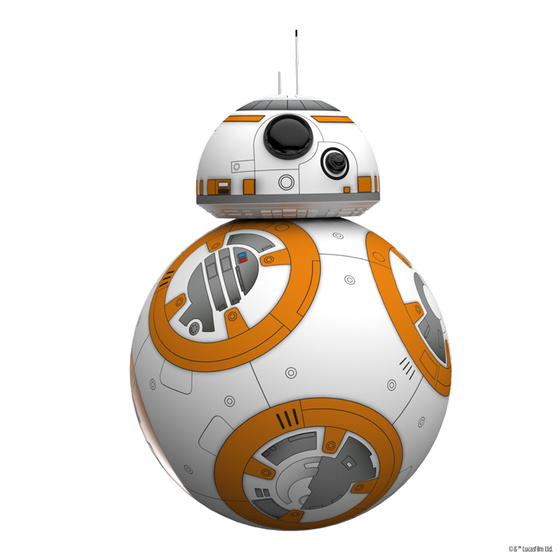
\includegraphics[scale=0.06]{robot}};
      \fill (1,-4)  rectangle (2,1);
      \fill (2,-3)  rectangle (3,0);%\atorig
	 \pgfmatrixnextcell
      \fill (-3,0)  rectangle (1,1);%\atorig2 
	 \pgfmatrixnextcell
      \fill (-1,-4) rectangle (0,-1);%\atorig3 
	 \pgfmatrixnextcell
      \fill (0,-1) rectangle (-1,-3);%\atorig4 
	 \pgfmatrixnextcell %ici pour un carré
      \fill (4,-3) rectangle (5,1);
      \fill (1,3.5) rectangle (6,2.5); 
      \fill (-1,0.5)  rectangle (4,1.5);%\atorig5
      \fill (3,-1) rectangle (4,-3);
	  \pgfmatrixnextcell 
	 \node[] at (-3,2) {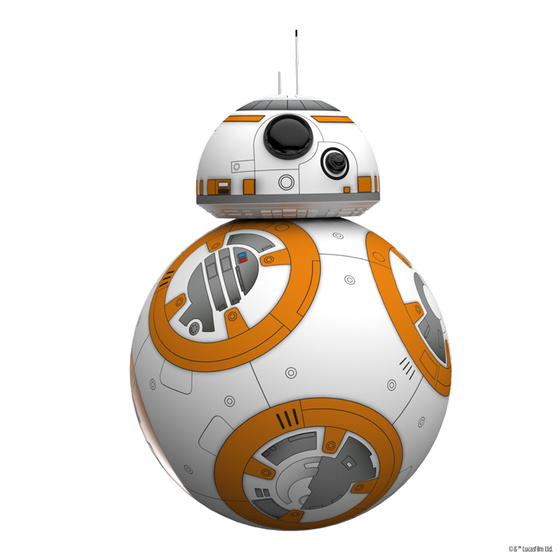
\includegraphics[scale=0.06]{robot}};
      \fill (0,-1)  rectangle (2,0);%\atorig6 
      \fill (-2,-2) rectangle (0,-1);
	  \pgfmatrixnextcell
      \fill (0,0)   rectangle (1,-4);%\atorig7 
	  \pgfmatrixnextcell
\node[] at (-2,-3) {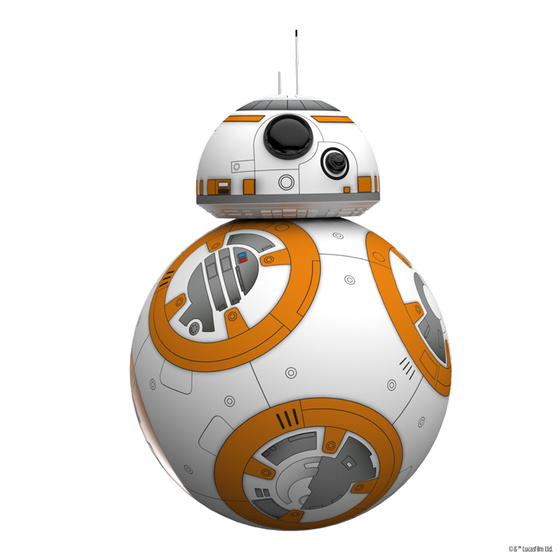
\includegraphics[scale=0.06]{robot}};
      \fill (1,-2) rectangle (2,2); \\
	   % \pgfmatrixnextcell
    }
\end{tikzpicture}
\caption{Exemple d'applications pour robots mobiles}
\label{fig:port:resume}
\end{figure}
Ils doivent se coordonner pour contrôler des
% tenir éloignés les voleurs des
conteneurs de marchandises, en vérifiant régulièrement qu'aucun d'eux
n'a été ouvert. Si un intrus est repéré, les robots doivent le
repousser à l'extérieur du périmètre de sécurité, puis retourner
surveiller les conteneurs. 

Un système constitué d'une telle équipe est appelé \emph{système
  distribué} ou \emph{réparti} \cite{Lynch96,Tel:2001:IDA:517021}. Ce
qualificatif de ``distribué'' provient du fait que le système est
composé d'un ensemble d'entités de calcul autonomes dotés de capacités
de communication qui leur permettent de résoudre une tâche commune.
Traditionnellement, les entités sont immobiles et communiquent les
unes avec les autres par passage de messages.  Le modèle de robot que
nous étudions dans cette thèse diffère du modèle classique par deux
aspects: les entités sont mobiles et ne communiquent pas par passage
de messages. Par ailleurs, ces entités mobiles peuvent être dotés de
capacités limitées.

Les travaux menés sur les réseaux de robots mobiles s'intéressent aux
caractéristiques de bases qui sont nécessaires afin que l'équipe de
robots puisse accomplir une tâche donnée, en l'absence de toute
autorité centrale. Ces travaux considèrent des déplacements des robots
dans un plan euclidien ou dans un environnement discret.  Les tâches
données peuvent être critiques, il faut donc veiller à ce que les
robots les accomplissent correctement, en dépit de leurs limitations.

Jusqu'à présent, les réseaux de robots ont été étudiés de manière
empirique et la plupart des résultats ont été validés seulement par
des preuves faites ``à la main''. Ces preuves visent à vérifier que
l'objectif des robots, appelé \emph{spécification} du problème et
décrit par un ensemble de propriétés, est satisfait. Elles sont
difficiles à lire et à écrire, car le raisonnement sur des systèmes
complexes est à la fois lourd et source d'erreurs.  L'utilisation de
preuves automatiques, basées sur un modèle mathématique abstrait du
système, pourrait simplifier ce processus de vérification. Pour ces
techniques de vérification formelle, plusieurs approches existent :
\begin{itemize}
\item La \emph{génération automatique de tests} prend en entrée
  une description formelle des comportements souhaités du système et
  génère un ensemble de tests à effectuer, qui doit couvrir un
  ensemble de comportements le plus grand possible. Le système est
  ensuite exécuté conformément à ces tests, et l'on peut vérifier si
  les sorties sont identiques à celles attendues.  Cependant il n’est
  pas toujours possible de fournir un ensemble exhaustif de tests, et
  la conception de tests est difficile pour les systèmes concurrents
  ou distribués.
%
\item La \emph{démonstration automatique} laisse l’ordinateur prouver
  automatiquement des théorèmes décrivant les propriétés du système,
  en se basant sur une description mathématique du programme, et sur
  un ensemble de règles de déduction et d’axiomes.  Cette méthode
  n’est cependant pas totalement automatisable, et l’assistant de
  preuves a besoin d’être plus ou moins guidé par une aide humaine
  pendant le processus. D'ailleurs, quand une preuve échoue, il est
  difficile d'en connaitre la raison. Divers assistants de preuve ont
  émergé depuis les années 60, par exemple PVS
  \footnote{http://pvs.csl.sri.com}, Coq
  \footnote{https://coq.inria.fr/} et Isabelle/HOL \footnote{https:
    //isabelle.in.tum.de} sont parmi les plus largement utilisés.
\item Le \emph{model-checking} part d’une représentation abstraite (un
  \emph{modèle}) du programme et d’une spécification formelle des
  comportements souhaités, et vérifie de façon exhaustive et
  automatique que tous les comportements du modèle satisfont cette
  spécification. Bien sûr, la recherche n’est exhaustive que sur
  l’abstraction du système considérée.  Un avantage de cette technique
  est sa complétude et sa capacité à extraire des comportements
  invalidant les propriétés. Ainsi, le \emph{model-checking} peut être
  utilisé dès la phase de conception pour valider les prototypes du
  système. L'explosion combinatoire est l'inconvénient majeur de cette
  méthode : explorer symboliquement toutes les exécutions (l'ensemble
  peut être infini) dans un modèle de grande taille est très
  consommateur de temps et de mémoire. Les
  models-checkers \textsc{Uppaal} \footnote{http://www.uppaal.org} et
  \textsc{Spin} \footnote{http://spinroot.com/spin/whatispin.html}
  sont parmi les plus connus.
\end{itemize}
Chacune de ces approches a ses avantages et ses inconvénients : alors
que les tests peuvent être faciles à mettre en œuvre, ils ne peuvent
pas être appliqués dans la phase de conception, et la génération de
tests exhaustifs est difficile.  Les preuves sont difficiles à mettre
en œuvre car elles nécessitent la présence d'un expert, mais elles
sont exhaustives, applicables dés la phase de conception, et peuvent
s'appliquer à des systèmes dits \emph{paramétrés}, où certaines
variables ne sont pas spécifiées, comme par exemple le nombre de
processus. Enfin, le \emph{model checking} est une approche globale et
automatique, mais limitée par la taille du modèle.  En outre, le
problème du \emph{model checking} de systèmes paramétrés est
indécidable en général~\cite{apt.kozen.86}.

Alors que le \emph{model checking} vérifie qu'un modèle satisfait une
propriété, la \emph{synthèse} consiste à se donner une spécification
et à générer, si possible, un modèle qui la satisfasse. 
% mise en oeuvre à la fin du processus de création d'un algorithme, 
% on souhaite que les méthodes formelles apparaissent au début du processus 
% de création.  La synthèse automatique d'algorithmes est une méthode
%formelle qui permet de générer un algorithme à partir de sa
%specification. 
L'avantage de cette méthode est qu'elle se situe en amont de la
conception et que les protocoles ainsi générés sont corrects par
construction.  Les premiers travaux sur la synthèse remontent à
Church~\cite{Church62} et ont été développés ensuite
dans~\cite{BuchiLandweber69,emersonclarke1981,
  MannaWolper84,PnueliR90}.
%It is even more difficult when the program to generate is intended 
%to work as an open system, maintaining an on-going interaction 
%with a (partially) unknown environment. 
Formellement, le problème de décision est le suivant : étant donnée
une spécification, existe-t-il un modèle qui la satisfasse ? Le
problème de synthèse proprement dit consiste, lorsque la réponse est
positive, à construire effectivement le modèle.

Dans le cas de systèmes ouverts, qui interagissent avec un
environnement, Buchi et Landweber \cite{BuchiLandweber69} ont montré
que le problème était décidable dans le cadre de la théorie des jeux.
Cette approche consiste à considérer le problème de synthèse comme un
\emph{jeu} entre le système et l'environnement. Le système et son
environnement sont deux joueurs qui s'affrontent, et le système gagne
s'il satisfait la spécification initiale. Ainsi, trouver un modèle qui
satisfait la spécification revient à trouver une stratégie gagnante
pour le système, quel que soit les stratéges de l'environnement.
% Ensuite, le
% problème classique en théorie des jeux qui consiste à trouver des
% stratégies gagnantes pour les joueurs est équivalent à trouver comment
% le système doit agir dans toutes les situations, afin de toujours
% satisfaire ses spécifications. 
Toutefois, ce problème est aussi indécidable en général pour les
systèmes distribués, la décidabilité étant obtenue avec des
hypothèses supplémentaires sur l'architecture~\cite{PnueliR90}.

Dans ce travail, notre objectif est d'étudier comment les méthodes
formelles peuvent être appliquées dans le contexte d'algorithmes de
robots mobiles.  Après une présentation de ces algorithmes, nous
montrons les avantages de ces méthodes par rapport aux approches
traditionnelles.



\section{Robots Mobiles}
Dans cette thèse nous nous sommes intéressés à un modèle théorique
\cite{suzuki_distributed_1999,FPS12} dans lequel les robots qui
coopèrent pour atteindre un objectif commun ont des capacités
limitées.  Les robots fonctionnent selon un cycle composé de trois
phases: \emph{Look, Compute} et \emph{Move}. Quand un robot exécute la
première phase, il examine l'environnement qui l'entoure et s'inscrit
dans un repère constitué par l'ensemble des autres robots. Dans la
deuxième phase, il calcule un futur mouvement en fonction de sa
position relative aux autres robots, et enfin, dans la dernière phase,
il met en \oe{}uvre le mouvement calculé précédemment.
 
Ce modèle, appelé SYm (ou ATOM), correspond à un comportement
synchrone des robots, qui exécutent ensemble chacune des
phases. Il a été étendu par Prencipe~\cite{prencipe_new_2000} afin
de prendre en compte un comportement asynchrone plus réaliste pour des
systèmes distribués. Ce nouveau modèle porte le nom de CORDA.  Ces
modèles diffèrent par leurs degrés d'atomicité:
\begin{itemize}
\item Dans le modèle historique, ATOM \cite{suzuki_distributed_1999},
  un sous ensemble de robots exécute chacune des trois phases de manière
  atomique. Il existe deux variantes : Fsync (Fully-synchronous) où tous
  les robots sont synchronisés, et Ssync (Semi-synchronous) où à
  chaque cycle, seul un sous-ensemble de robots s'exécute de manière
  synchrone.

  Dans ce modèle, le comportement du système correspond à l'exécution
  de toutes les opérations instantanément, la conséquence est qu'aucun
  robot ne pourra jamais être observé alors qu'il se déplace, et la
  compréhension de l'univers par les robots actifs est toujours
  cohérente.
\item Le second modèle, CORDA~\cite{prencipe_new_2000} ou Async, est
  une variante moins contrain\-te et donc plus réaliste, où chaque robot
  peut être activé de manière asynchrone, indépendamment des autres
  robots. La durée de chaque phase, et le temps entre les phases
  successives d'un même cycle sont limitées mais inconnues. En
  conséquence, les calculs peuvent être basés sur des observations
  totalement obsolètes, prises arbitrairement loin dans le passé.
\end{itemize}
Notons qu'en terme d'exécutions, Fsync est inclus dans Ssync et Ssync
est inclus dans Async.  \bigskip

La capacité d'une équipe à réaliser une tâche assignée dépend
principalement de ses membres et de leurs capacités: plus les robots
sont puissants, plus le problème est résolu facilement. Les robots du
modèle considéré ici disposent quant à eux de capacités très limitées.
Nous allons maintenant détailler les hypothèses minimales généralement
faites sur les capacités de ces robots.
 
%They are endowed with sensing, computing, 
%and moving capabilities described below. 
\subsection{Des robots restreints}
%Anonymous and similar: 
Les robots sont identiques et anonymes, ils exécutent le même
algorithme et ils ne peuvent pas être distingués par leur apparence,
mais ils peuvent avoir des vitesses de calcul et de déplacement
différentes (dans le cas asynchrone). De plus ces robots peuvent avoir
des identités mais ni eux ni les autres robots n'ont connaissance ou
accès à ces identités.

%oblivious
Les robots sont amnésiques \ie ils n'ont aucun souvenir de leurs
actions
passées. % de leurs actions ne dépendent pas des actions précédentes.
Cette carctéristique implique que tout état peut être considéré comme
initial. Par conséquent, les algorithmes de robots sont
auto-stabilisants : un algorithme distribué est dit \emph{auto-stabilisant}
s'il assure qu'un comportement correct peut être retrouvé en un temps
fini sans aucune aide exterieure.
%In~\cite{DieudonneP12}, Dieudonne et Petit discuss 
%on the link between the mobile robot model and self-stabilization.

%no common handedness: 
Les robots n'ont pas un sens commun de l'orientation.  Chaque robot a
sa propre unité de longueur, et possède une boussole locale
définissant son propre système de coordonnées cartésiennes locales. Ce
système de coordonnées local est auto-centré, \ie l'origine est la
position du robot. De plus, le système de coordonnées local des robots
peut complètement changer à chaque cycle, mais il reste invariant au
cours d'un cycle.

%no communication; other works communication: via msg, pebbles, ...
Les robots sont silencieux : il ne communiquent pas entre eux de
manière explicite, mais seulement en observant les positions des
autres robots, et prennent leurs décisions en conséquence. En d'autres
termes, le seul moyen pour un robot d'envoyer des informations à un
autre robot est de se déplacer et de laisser les autres robots
observer son mouvement avant de bouger à nouveau.

Bien que dans la littérature des robots plus faibles soient étudiés,
nous nous sommes intéressés dans cette thèse aux robots décrit par le
modèle original de Suzuki et Yamashita \cite{suzuki_distributed_1999}.

\subsection{Les capacités des robots}
Pour exécuter leurs cycles Look-Compute-Move, les robots peuvent
observer leur environnement, prendre des décision et se mouvoir.  Deux
types d'environnements ont été étudiés :
\begin{itemize}
\item  le plan euclidien (continu) \cite{suzuki_distributed_1999,FPS12},
%dans lequel les robots évoluent dans le plan; 
\item un environnement
  discret~\cite{KlasingMP06,flocchini_computing_2007}, représenté par
  un graphe, dans lequel les noeuds correspondent aux différentes
  positions possibles et les arcs aux routes permettant aux robots
  d'aller d'une position à une autre.
\end{itemize}
La représentation discrète est motivée par des aspects pratiques liés
au manque de fiabilité des dispositifs d'observation utilisés par les
robots ainsi qu'à l'imprécision de leur
motorisation~\cite{CDDMJ08j}. Cela permet notamment de simplifier la
conception des modèles en raisonnant sur des structures
finies. Cependant, ce cadre rend le modèle plus sensible à
la taille des constantes, ce qui peut augmenter de manière
significative le nombre de configurations symétriques lorsque le
graphe sous-jacent est également symétrique (par exemple un anneau) et
donc la taille des preuves de correction~\cite{ASN11c, KLOT11,
  KLOT12}.

\subsubsection{Observation}
\index{Visibility} Les robots sont dotés de capteurs de vision
fournissant les emplacements des autres robots. L'emplacementCette
information est obtenue soit avec un grain fin (donc un certain degré
de précision), soit avec un grain. Dans le premier cas, la littérature
se réfère principalement au modèle où l'espace est continu, tandis que
dans le second cas l'environnement est discret.

Les robots n'ont pas de dimension et donc leur visibilité ne peut être
obstruée: si trois robots $r_1$, $r_2$, et $r_3$ sont alignés, avec
$r_2$ au milieu, $r_1$ peut quand même voir $r_3 $. Les robots peuvent
théoriquement partager la même position : cette formation est appelée
une \emph{tour} \cite{FPS12}. La capacité pour un robot de détecter la
multiplicité est essentielle pour réaliser certaines tâches
particulières. Parmi les détecteurs de multiplicité, nous distinguons :

\begin{itemize}
\item les détecteurs \emph{faibles}, capables de déterminer s'il y a
  zéro, un ou plusieurs robots à une position particulière,
\item les détecteurs  \emph{forts} qui fournissent le nombre exact
  de robots à une position particulière.
\end{itemize}
Le capteur correspondant peut être local ou global : dans le contexte
local un robot ne détecte que la multiplicité à sa position courante,
alors que dans le cadre global le nombre de robots sur chaque position
est connu.  Dans le modèle que nous étudions il n'y a aucune
restriction sur la distance de visibilité des robots.

\subsubsection{Calcul}
Comme dans les systèmes distribués classiques, les robots sont
supposés être en mesure d'effectuer toute suite finie de calculs en
temps négligeable. Comme les robots sont amnésiques, la mémoire
volatile est utilisée pour effectuer le cycle Look-Compute-Move, le
contenu de la mémoire est effacé à la fin de chaque cycle.  Le calcul
prend en entrée l'observation faite dans la phase Look et retourne un
movement.  Lorsque deux robots sont sur la même position ou sont
symétriques, ils calculent le même mouvement.

\subsubsection{Mouvement}
Les robots peuvent se déplacer seulement à l'emplacement déterminé par
la phase de calcul du cycle en cours. Dans certains cas, en raison de
la symétrie, la position calculée peut être ambiguë : elle correspond
alors à un mouvement non déterministe, qui peut être résolu par un
ordonnanceur. Dans le modèle discret, un robot peut se déplacer
seulement vers un emplacement adjacent à sa position
courante. Dans le modèle continu, un robot se déplace vers sa
destination quelle qu'elle soit.

%schedulers %%%%%%%%%%%%%%fairness%%%%%%%%%%%%
\subsubsection{Ordonnancement}
\index{Fairness} Lorsque plusieurs processus veulent s'exécuter
simultanément, il est nécessaire de determiner lequel sera exécuté et
à quel moment.  Les ordonnanceurs sont des abstractions utilisées pour
caractériser le degré d'asynchronisme des
robots~\cite{DefagoGMP06,FPS12}.  Un ordonnanceur \emph{équitable} est
généralement utilisé, il active tous les robots infiniment souvent,
%afin d'éviter la famine, 
mais certains robots peuvent être activés
arbitrairement plus que les autres.

Il existe d'autres types d'équité qui dépendent de l'ordonnancement
des actions plutôt que des processus.  Un ordonnanceur \emph{fort}
garantit que chaque action tirable infiniment souvent possible sera
exécutée infiniment souvent. Un ordonnanceur \emph{faible} garantit
que chaque action tirable continûment à partir d'un certain moment
sera exécutée une infinité de fois.
 

\bigskip Dans cette thèse, nous considérons des robots dans un univers
discret.  Nous nous sommes principalement intéressés à deux problèmes
largement étudiés pour les robots mobiles et autonomes : le premier
est celui du rassemblement \cite{markoubook}, où les robots doivent se
retrouver sur une unique position, le second est celui de
l'exploration \cite{flocchini_computing_2007,
  devismes_optimal_2010-1}, où les robots doivent visiter tous les
noeuds du graphe.

Le problème du rassemblement est le premier à avoir été étudié dans la
littérature, aussi bien
historiquement~\cite{suzuki_distributed_1999,KlasingMP06,
  klasing_taking_2008,Pelc11} que par le nombre de publications.
Quelles que soient leurs positions initiales, les robots doivent se
déplacer afin d'être finalement tous regroupés sur une même position,
non connue à l'avance, et y rester par la suite.  Comme le problème de
consensus dans les systèmes distribués classiques, où toutes les
entités doivent se mettre d'accord sur une même valeur, le
rassemblement a une définition simple, mais l'existence d'une solution
dépend du degré de synchronisme du système.

Un équipe de robot a exploré un graphe si chaque position de celui-ci
est visité par au moins un robot.  Le problème de l'exploration a
plusieurs variantes, parmi lesquelles nous avons étudié l'exploration avec
arrêt et l'exploration perpétuelle exclusive.  L'exploration avec
arrêt est la version historique du travail sur l'exploration
\cite{flocchini_computing_2007,lamani_optimal_2010,devismes_optimal_2010-1}.
Les robots doivent atteindre une configuration dans laquelle ils sont
tous inactifs et où chaque noeud du graphe a été visité par au moins
un robot. La difficulté de cette tâche réside dans le fait que les
robots doivent s'arrêter une fois l'exploration faite. En l'absence de
mémoire persistante, cela signifie qu'ils doivent être en mesure de
faire la distinction entre les différentes étapes du processus
d'exploration.  L'exploration perpétuelle exclusive a été étudiée plus
récemment \cite{blin_exclusive_2010, navarraipdps2013}.  Chaque noeud
du graphe doit être visité infiniment souvent et aucun point de
multiplicité ne doit apparaître.
	
%%%%%%%%%%%%%%%%%%%%%%%%%VERIFICATION%%%%%%%%%%%%%%%%%%%%%%%%%%%%%
\section{Méthodes formelles et algorithmes de robots}
L'utilisation de méthodes formelles exige des représentations
mathématiques du système et de sa spécification, donnée comme un
ensemble de propriétés.  Un système distribué est souvent décrit comme
un système de transition \cite{Tel:2001:IDA:517021,
  DBLP:books/mk/Lynch96}, composé des modèles de ses sous-systèmes.
Les propriétés peuvent être classées en différents types, parmi
lesquels les propriétés de sûreté et de vivacité. Les propriétés de
sureté exigent que \og{}quelque chose de mauvais ne se produise
jamais\fg{}, comme l'absence de blocage dans l'exécution d'un système.
Les invariants forment une sous-classe importante des propriétés de
sûreté, exprimant que \og{}quelque chose est vrai à chaque étape de
chaque exécution\fg{}.  Les propriétés de vivacité exigent que
\og{}quelque chose de bon finisse par arriver\fg{}, par exemple que 
% qu'il n'y aura pas de famine, 
chaque processus ait finalement accès aux ressources critiques.  Toute
spécification peut être écrite comme la conjonction de propriétés de
sécurité et de vivacité \cite{AlpernS85}.
		

\subsection{Model-checking}
Un \emph{model-checker} prend en entrée un modèle $M$, souvent sous la
forme d'un système de transitions, décrivant toutes les exécutions
possibles du système, et la propriété à vérifier, exprimée par une
formule logique $\varphi$. Il détermine si le modèle satisfait ou non
la formule. Lorsque la propriété n'est pas satisfaite, le
\emph{model-checker} fournit un contre-exemple, \ie une exécution du
modèle qui invalide la propriété. Ce contre-exemple est utile pour
trouver des erreurs dans les systèmes complexes, c'est un avantage
majeur du model-checking par rapport aux autres méthodes formelles,
comme la démonstration de théorèmes, qui peuvent infirmer une
propriété, mais sans fournir systématiquement un tel contre-exemple.

%\todo{The automata approach}
L'approche par automates pour le \emph{model-checking} a été
introduite par Vardi et Wolper~\cite{vardi_automata-theoretic_1986},
afin de fournir un cadre unifié et extensible, d'abord appliqué à une
classe de formules logiques appelée \textsf{LTL}.  Cette approche
comprend trois étapes :
\begin{itemize}
\item Tout d'abord le système et ses spécifications doivent être
  modélisés. Soit $M$ le modèle du système, et $\varphi$ la formule
  \textsf{LTL} représentant la spécification du système.  Le langage
  $\mathcal{L} (M)$ associé à $M$ représente toutes les exécutions de
  $M$.  La négation de la formule $\varphi$ est traduite en un
  automate $\mathcal{A}_{\neg \varphi}$ dont le langage,
  $\mathcal{L}(A_{\neg \varphi})$, est l'ensemble des exécutions qui
  invalident $\varphi$.
\item Les automates $M$ et $\mathcal{A}_{\neg \varphi}$ sont
  synchronisés afin d'obtenir un automate $M \times \mathcal{A}_{\neg
    \varphi}$ dont le langage $\mathcal{L}(M \times \mathcal{A}_{\neg
    \varphi}) = \mathcal{L} (M) \cap \mathcal{L} (\mathcal{A}_{\neg
    \varphi})$, est l'ensemble des exécutions de $M$ qui invalident
  $\varphi$.
\item Enfin, le \emph{model-checker} effectue un test de vacuité
  sur le produit. Le modèle $M$ satisfait $\varphi$ si et seulement si
  $\mathcal{L} ( M \times \mathcal{A}_{\neg \varphi}) = \emptyset$.
  Si le test de vacuité est positif, cela veut dire qu'aucune
  exécution n'invalide $\varphi$, les propriétés exprimées par
  $\varphi$ sont donc satisfaites par le modèle $M$. Sinon, une
  exécution de $M$ qui invalide $\varphi$ est retournée comme
  contre-exemple.
\end{itemize}		

L'inconvénient de cette méthode est le problème bien connu
d'\emph{explosion combinatoire}~\cite{Valmari96}, lorsque le produit
$M \times \mathcal{A}_{\neg \varphi}$ est de grande taille.  En
particulier, lorsque le modèle $M$ du système est lui-même obtenu par
produit de plusieurs composants, sa taille est exponentielle en le
nombre de processus. Ainsi, dans l'approche par automates, le produit
est souvent trop grand pour que le test de vacuité puisse être réalisé
dans un délai raisonnable en terme de temps d'exécution ou de mémoire
utilisée.

Les systèmes distribués sont naturellement structurés comme un
ensemble de plusieurs processus, parmi lesquels certains présentent
des comportements similaires. De tels composants sont dits
symétriques, et connaître le comportement d'un de ces composants est
souvent suffisant pour connaître le comportement de ses pairs. Plus
formellement, les symétries du système définissent une relation
d'équivalence sur ses états, qui permet de construire un espace
d'états réduit, par quotient, où au moins un état par classe
d'équivalence est maintenu.  Si un seul représentant par classe est
maintenu, la réduction maximale est atteinte. La définition de
symétries garantit que l'espace d'états réduit préserve les
propriétés, si les symétries sont respectés~\cite{ClarkeJEF96,
  EmersonS96}. Cette réduction est généralement exponentiellement plus
petite que l'espace d'états initial, ce qui réduit le temps
d'exécution et la mémoire utilisée lors la procédure de vérification.

À notre connaissance, dans le contexte des réseaux de robots mobiles
opérant dans l'espace discret, une seule tentative, par Devismes
\emph{et al.}~\cite{devismes_optimal_2011}, a étudié la possibilité
d'utiliser le model-checking comme méthode de vérification. Les auteurs
utilisent LUSTRE~\cite{lustre:ieee} pour décrire et vérifier le
problème de l'exploration avec arrêt sur une grille de taille $ 3
\times 3 $, par $3$ robots, dans le modèle Ssync.  Ils considèrent un
type particulier de configurations avec une tour de 2 robots et un
robot isolé, où seul le robot isolé souhaite se déplacer.  Ils
vérifient l'invariant: \emph{nœuds visités} $\leq 4 $, ce qui leur
permet de compléter leurs preuves manuelles par de la vérification
formelle pour ce cas précis.
	
\subsection{Preuves}
En utilisant un assistant de preuves, un utilisateur peut exprimer des
données, des programmes, des théorèmes et des preuves.  Les assistants
de preuves fournissent une garantie supplémentaire en vérifiant
mécaniquement la solidité de la preuve une fois qu'un expert l'a
développée de manière interactive.  Ils ont été utilisés avec succès
pour diverses tâches telles que la formalisation de la sémantique des
langages de programmation \cite{Leroy09}, la certification d'un noyau
de l'OS \cite{KleinAEHCDEEKNSTW10}, ou la vérification de protocoles
cryptographiques \cite{AlmeidaBBBKB12}.  Au cours des vingt dernières
années, l'utilisation d'assistants de preuves automatiques s'est
étendue à la validation de systèmes distribués.

L'inconvénient majeur de cette méthode est qu'elle nécessite un fort
niveau d'expertise pour l'écriture de la preuve. De plus elle n'est
pas complètement automatique, car les preuves sont souvent obtenues à
partir de nombreux lemmes.

Pour le modèle de robots, Courtieu \emph{et al.} ont utilisé COQ afin
de certifier des résultats d'impossibilité, en présence
de processus byzantins \cite{AugerBCTU13}. Une preuve certifiée du
résultat de \cite{suzuki_distributed_1999} est proposé
dans \cite{CourtieuRTU15}, confirmant l'impossibilité de regrouper deux
robots. Les auteurs fournissent également un résultat plus général
d'impossibilité : rassembler un nombre pair de robots, lorsque deux
robots sont initialement sur la même position, est impossible.
		
\subsection{Synthèse d'algorithmes}
%Même s'il est utile de vérifier/ prouver des algorithmes existants,
Les techniques de synthèse sont situées plus en amont, puisqu'elles
permettent, dans certains cas, de générer automatiquement un
algorithme correct.  Pour cela, soit $\varphi$ la spécification que le
système doit satisfaire, et soit $E$ un modèle de l'environnement.  Le
problème de synthèse cherche s'il existe un programme $P$ tel que $P
\times E$ satisfait $\varphi$. Ainsi, le système décrit par $P$atteint
son objectif, quel que soit le comportement de l'environnement.
% la synthèse prend en entrée la
% spécification d'un système interagissant avec un environnement, et
% demande s'il existe un programme qui satisfasse cette spécification,
% quel que soit le comportement de l'environnement.
Lorsque la réponse est positive, le programme doit alors être
construit.  Une réponse négative donne une preuve qu'il y a toujours
une façon pour l'environnement d'empêcher le système d'atteindre son
objectif. Une telle stratégie de l'environnement peut donc être vue
comme une preuve d'impossibilité.

%  Le comportement du système ainsi créé doit
% correspondre exactement à tous les comportements admissibles par la
% spécification.

Au premier abord on pourrait croire que le modèle réellement
nécessaire est celui des \emph{jeux distribués}, dans lequel chaque
robot représente un joueur distinct, tous ces joueurs coopérant contre
un environnement hostile. Dans les jeux distribués, l'existence d'une
stratégie gagnante pour l'équipe de joueurs est indécidable
\cite{PetersonReif79}. Cependant, le fait que les robots soient
capables de voir leur environnement, et donc de toujours connaître la
configuration du système, nous permet de rester dans le cadre de jeux
à deux joueurs. Il est donc possible de coder l'ensemble des robots comme
un seul joueur.  Bien sûr, la stratégie obtenu sera centralisée, le
jeu devra être conçu afin de n'obtenir que des stratégies qui peuvent
être distribuées afin d'être implémentées sur les robots.

À notre connaissance, dans le contexte des réseaux de robots mobiles,
une seule tentative \cite{BDPPT12c} examine la possibilité de
synthétiser automatiquement des protocoles de robots mobiles.  Ce
travail considère l'exploration perpétuelle exclusive par $k$ robots
d'anneaux de tailles $n$ quelconque dans le modèle Ssync.  L'approche
choisie est \emph{brute force} : tous les protocoles possibles sont générés
mécaniquement sans qu'aucune propriété à satisfaire ne soit
spécifiée. Les protocoles ainsi obtenus ne contiennent aucune
\emph{ambiguïté}, c'est à dire qu'ils ne contiennent pas de
configurations symétriques, ni de de multiplicité.  Une fois ces
protocoles construits chacun est étudié manuellement afin de voir s'il
permet ou non une exploration perpétuelle exclusive. Tous les
protocoles qui le permettent sont ensuite comparés afin d'obtenir une
étude qualitative.

Dans cette thèse nous avons voulu donner suite à ces travaux, en
démontrant que le model-checking pouvait être utilisé dans les réseaux
de robots afin de vérifier des instances de protocoles entiers et non
seulement comme aide pour des preuves manuelles.  Nous avons voulu
également montrer le pouvoir de la synthèse qui permet de générer
automatiquement des algorithmes corrects par construction sans se
restreindre sur les mouvements ou les configurations possibles.  Notre
approche diffère des précédentes, car notre modèle est suffisamment
général pour décrire tous les modèles d'atomicité, alors que les
travaux antérieurs ne gèrent que les modèles synchrones.



\section{Contributions}
		%\todo{model}
Nous proposons un modèle formel représentant un réseau de robots
mobiles comme un produit d'automates.  Ce modèle permet de décrire les
trois hypothèses d'exécution décrites ci-dessus, à savoir Fsync, Ssync
et Async. Nous en réalisons une implémentation qui permet de réduire
la taille de l'espace d'états en utilisant les symétries du modèles.

Grâce à ce modèle, nous produisons deux contributions, relatives à la
vérification et à la synthèse.

\paragraph{Vérification.} Nous avons tout d'abord vérifié formellement
certaines instances de deux protocoles existants, qui permettent de
résoudre les deux variantes de l'exploration d'anneau avec des robots
asynchrones.  Afin de vérifier les algorithmes de robots évoluant sur
un anneau, nous avons créé un générateur de modèles qui,
indépendamment de la tâche à effectuer, prend en entrée la taille de
l'anneau, le nombre de robots, le modèle d'exécution du système et un
algorithme à vérifier sous la forme de transitions gardées, puis
construit le modèle du système. Une fois les spécifications du système
formellement énoncées, l'utilisation d'un model-checker nous permet de
vérifier l'algorithme pour une taille d'anneau et un nombre de robots
fixés.  Nous avons d'abord vérifié le protocole de Flocchini \emph{et
  al} qui résout le problème de l'exploration avec arrêt \cite{
  flocchini_computing_2007}, puis nous avons étudié le problème de
l'exploration perpétuelle exclusive avec l'algorithme de Blin \emph{et
  al} \cite{blin_exclusive_2010}. Dans les travaux d'origines, les
deux protocoles ont été donnés par une suite de descriptions
informelles, que nous avons dû formaliser.

$\bullet$ Dans le cas de l'exploration avec arrêt
\cite{flocchini_computing_2007}, l'algorithme a été prouvé correct
grâce à une preuve manuelle lorsque le nombre de robots est $k > 17 $
et $ n $ (la taille de l'anneau) et $ k $ sont premiers entre eux.  La
nécessité de la borne $k > 17 $ n'ayant pas été prouvée dans le papier
d'origine, notre méthodologie démontre que pour de nombreux cas de $k
$ et $ n $ non couverts dans le document original, le protocole est
toujours correct. Nous proposons une conjecture pour les cas avec $ k
\leq 17 $ robots.
 
$\bullet$ Nous avons ensuite étudié l'algorithme de Blin \emph{et al } qui
permet à un nombre minimal de $3$ robots d'explorer perpétuellement un
anneau sans que des collisions ne surviennent
\cite{blin_exclusive_2010}.  Dans ce cas, notre méthodologie a permis
d'obtenir un contre-exemple relevant d'un défaut subtil dans
l'algorithme, lorsque celui est exécuté dans le modèle asynchrone.
Nous proposons une correction du protocole original et vérifions par
\emph{model-checking} plusieurs instances du nouvel algorithme. Nous
terminons cette étude en donnant une preuve inductive de ce protocole
pour des anneaux de tailles quelconques.

\paragraph{Synthèse.} La deuxième contribution de cette thèse porte
sur la synthèse automatique de protocoles pour les réseaux de robots.
Notre but est de montrer comment réaliser la synthèse de protocoles de
rassemblement pour des robots évoluant dans un environnement discret.
Nous avons examiné séparément les modèles synchrones et asynchrones.

$\bullet$ Nous avons d'abord proposé un encodage du problème de
rassemblement par un jeu d'accessibilité avec deux joueurs : la
coalition de robot d'une part et son adversaire, qui est
l'ordonnanceur. L'adversaire décide également le sens de déplacement
des robots désorientés, à chaque activation. Notre encodage est assez
expressif pour englober les deux modèles synchrone Ssync et Fsync, y
compris lorsque plusieurs robots sont situés sur le même noeud et
lorsque des situations symétriques se produisent, contrairement à la
solution ad-hoc de \cite{BDPPT12c}.  Cela nous a permis de générer
automatiquement un algorithme distribué \emph{optimal}, pour trois
robots évoluant sur des anneaux de tailles fixes. Notre critère
d'optimalité se réfère au nombre de mouvements nécessaires pour que
les robots se regroupent.  En étudiant les solutions produites par
l'outil, nous avons pu extraire un \emph{motif}, et en déduire un
algorithme paramètré. Une preuve par induction nous a permis de
prouver que cet algorithme est correct pour toute taille d'anneau dans
le modèle synchrone mais aussi dans le modèle asynchrone.

$\bullet$ Dans le cas asynchrone, nous montrons comment la recherche
d'un algorithme de rassemblement de robots peut être vu comme un jeu à
deux joueurs avec information partielle.  Dans ce type de jeux,
contrairement aux précédents, les joueurs ont une vue incomplète du
système.  Afin de lutter contre l'explosion combinatoire due au modèle
asynchrone, nous proposons un algorithme récursif qui permet d'obtenir
un protocole de rassemblement, en combinant la synthèse d'algorithmes
dans le modèle synchrone avec le \emph{model checking} des solutions
produites, exacutées dans un modèle asynchrone.

	
	

\selectlanguage{english}
\addtocontents{toc}{\protect\setcounter{tocdepth}{2}}

% back cover
\pagestyle{empty}
\cleardoublepage
\pagestyle{empty}
\clearpage
%\input{abstractBack}
\end{document}